% main.tex : anonymous ICWSM submission, AAAI two-column format. Integrator file: no prose of its own.
%
% PAPER. What a Whisper-family pipeline does to the audio of recordings published by creators selected as channelling
%   mediums, and the registered, then amended, protocol for model-coded labels (registry 2026-11-21 02:50 UTC).
%   Plan: outline.md and the fix lists, kept in the private work folder (they hold private values). Writers: A (abstract, sections 1, 2, 9, 10, ethics,
%   appendix C), B (sections 3 to 5, appendix A), C (sections 6 to 8, appendix B).
%
% STYLE SOURCE. aaai25.sty and aaai25.bst beside this file were copied, unchanged, from the old draft
%   (paper/cohort-draft-2026-11-20), which took them from the arXiv e-print of arXiv:2512.17768 (ICWSM 2026).
%   SHA-256 aaai25.sty e062275ae269b957cba4d5b6b5afb189da8443a2645972b541a7d6eead0f6c65
%   SHA-256 aaai25.bst 78279b2c82d08ffb9d5fa2ae34c25496e84cdda85ddaa495dc44f5eafa3dae16
%   The preamble lines marked DO NOT CHANGE THIS are the AAAI author-kit lines of the old draft, unchanged.
%   ICWSM may issue a newer kit for the target year.
%
% NUMBERS. Every measured number is a macro of findings/numbers.tex, GENERATED by the private builder
%   build_numbers.py (each line names its source file and field). findings/pending.tex holds one macro per
%   placeholder of outline section 8; each expands to \pending{...} until a later build fills it from its source.
%   findings/results.tex holds the first-round results from the public results file (pending without it).
%   None of these files is edited by hand. floats/*.tex (tabulars) and floats/*.pdf (figures) come from the same builder.
%
% BUILD. bash build.sh   (or: latexmk -pdf main.tex ; or pdflatex main ; bibtex main ; pdflatex main ; pdflatex main)

\documentclass[letterpaper]{article} % DO NOT CHANGE THIS
\usepackage[submission]{aaai25}  % DO NOT CHANGE THIS (submission option: anonymous, no copyright slug)
\usepackage{times}  % DO NOT CHANGE THIS
\usepackage{helvet}  % DO NOT CHANGE THIS
\usepackage{courier}  % DO NOT CHANGE THIS
\usepackage[hyphens]{url}  % DO NOT CHANGE THIS
\usepackage{graphicx} % DO NOT CHANGE THIS
\urlstyle{rm} % DO NOT CHANGE THIS
\def\UrlFont{\rm}  % DO NOT CHANGE THIS
\usepackage{natbib}  % DO NOT CHANGE THIS AND DO NOT ADD ANY OPTIONS TO IT
\usepackage{caption} % DO NOT CHANGE THIS AND DO NOT ADD ANY OPTIONS TO IT
\frenchspacing  % DO NOT CHANGE THIS
\setlength{\pdfpagewidth}{8.5in}  % DO NOT CHANGE THIS
\setlength{\pdfpageheight}{11in}  % DO NOT CHANGE THIS
\usepackage{booktabs}
\usepackage{array}
% Anonymous submission (privacy review P30, third round): no pdfTeX banner, file names or embedded figure info
% dictionaries in the PDF; build.sh sets the document dates in UTC.
\pdfsuppressptexinfo=-1

\setcounter{secnumdepth}{2} % numbered sections, as in the paper the style was taken from

% A placeholder for a number that does not exist yet (outline section 8). Never redefined to a number by hand.
\newcommand{\pending}[1]{\textbf{[pending: #1]}}

% numbers.tex: GENERATED by WORK/build_numbers.py (private generator) at 2026-11-22T01:51:42Z. Do not edit.
% One macro per line for every number the paper uses (unused macros are not written); the comment names
% the source (root-relative path) and the field.
% Roots: REV = review builds, R2R = panel round-2 runs, WER = word-error-rate anchor, LLM = labelling,
% DBL = second reading, V3R = cross-vendor check, REG = registry folder, OLD = old draft, PRIV = run folder.
% Percentages have no % sign; negatives use \ensuremath{-}; \pending{...} marks what cannot be computed yet.
% \pending is defined by main.tex after this file is read (macros expand only where used).

% --- 7.1 Build, design and registry stamps
\newcommand{\RegistryFrozenStamp}{20 November 2026, 19:47 UTC}% REG/registry.md : What is frozen : Frozen at
\newcommand{\HypothesesShaPrefix}{831ed6fa}% REG/registry.md; REG/hypotheses.md : frozen table : Text of the hypotheses
\newcommand{\HThreeFrozenStamp}{20:38 UTC}% REG/registry.md : Procedure freeze : H3 heading
\newcommand{\HThreeRunStamp}{20:39 UTC}% REG/registry.md : H3 table : Result
\newcommand{\FreezeOneStamp}{21 November 2026, 04:58 UTC}% LLM/freeze-20261121T045822Z.json : frozen_utc
\newcommand{\FreezeOneFiles}{128}% LLM/freeze-20261121T045822Z.json; REG/registry.md : len(sha256); registry '128 file hashes'
\newcommand{\FreezeOneConfigPrefix}{d95387a4}% LLM/freeze-20261121T045822Z.json : config_sha256[:8]
\newcommand{\ModelSmall}{gpt-6-luna}% LLM/freeze-20261121T045822Z.json : models.small
\newcommand{\ModelMiddle}{gpt-6.1-terra}% LLM/freeze-20261121T045822Z.json : models.middle
\newcommand{\ModelLarge}{gpt-6-sol}% LLM/freeze-20261121T045822Z.json : models.large
\newcommand{\ModelLargeGate}{gpt-6.2-sol}% LLM/design/gates-forecasts-content-titles-G.md : configuration table : FC large check : Model
\newcommand{\NAmendments}{11}% REG/registry.md : amendment headings **A<n>. (A10 entered 16:07 UTC)
\newcommand{\PlanShaPrefix}{061bab33}% REG/exploratory-reporting-plan-addendum-1.md : header : SHA-256 of exploratory-reporting-plan.md
\newcommand{\AddendumOneStamp}{05:30 UTC}% REG/exploratory-reporting-plan-addendum-1.md : header : written
\newcommand{\PlanRegisteredStamp}{06:36 UTC}% REG/registry.md : registry row : exploratory reporting plan registered
\newcommand{\EnglishFirstStamp}{05:52 UTC on 20 November}% REV/build-descriptive/out/D2/D2-run-order-paragraph.txt : paragraph : English-first start
\newcommand{\SnapLines}{1{,}213}% REG/registry.md : frozen table : Hold-out
\newcommand{\MinCreatorsRegistered}{12}% REV/build-robustness/out/R2/R2-calibration-eligibility-table.csv : H1 registered_not_run_below
\newcommand{\MinCreatorsOneSided}{8}% REV/build-robustness/out/R2/R2-calibration-eligibility-table.csv : H1 minimum_n_first_holm
\newcommand{\MinCreatorsTwoSided}{9}% REV/build-robustness/out/R2/R2-calibration-eligibility-table.csv : H2 minimum_n_first_holm
\newcommand{\NSkepticSearches}{147}% REG/hypotheses.md : 14.0 : skeptic
\newcommand{\NSeamSearches}{9}% REG/hypotheses.md : 14.1 N5(a) : arXiv searches by the skeptic whose abstracts were checked for the window position
\newcommand{\NIcwsmSearches}{four}% OLD/setup/setup-numbers.tex : NIcwsmSearches
\newcommand{\SpendMeasured}{125.93}% LLM/spend.jsonl : sum of usd over measured rows (kind not reserved/released)
\newcommand{\SpendCommitted}{126.70}% LLM/spend.jsonl : sum of usd over all rows (open reservations included)
\newcommand{\SpendStamp}{01:51 UTC on 22 November 2026}% LLM/spend.jsonl : read time (date -u)

% --- 7.11 Limitations, contacts and ethics
\newcommand{\ExtRequests}{396{,}608}% LLM/spend.jsonl : measured rows : requests (1 where a row has none)
\newcommand{\ExtInputTokensM}{731.5}% LLM/spend.jsonl : measured rows : input_tokens / 1e6
\newcommand{\ExtWordsM}{96.6}% LLM/spend.jsonl : 0.75 x uncached input tokens of corpus-text tags (D8 rule), / 1e6; an estimate
\newcommand{\ExtStamp}{01:51 UTC on 22 November 2026}% LLM/spend.jsonl : read time

% --- 7.1 Build, design and registry stamps
\newcommand{\FreezeOnePrefix}{c3b1161d}% REG/registry.md; LLM/freeze-20261121T045822Z.json : Freeze 1 table : Record SHA-256 prefix
\newcommand{\FreezeOneAmendStamp}{16:06 UTC}% REG/registry.md; LLM/freeze.json : Freeze 1, amendment 1 : heading time
\newcommand{\FreezeOneAmendPrefix}{c57e64db}% REG/registry.md; LLM/freeze.json : Freeze 1, amendment 1 : Record SHA-256 prefix
\newcommand{\ProduceOldPrefix}{60bd9f62}% REG/registry.md : Freeze 1, amendment 1 : produce.py before
\newcommand{\ProduceNewPrefix}{0497c5b5}% REG/registry.md : Freeze 1, amendment 1 : produce.py after
\newcommand{\FixtureRequests}{256}% REG/registry.md : Freeze 1, amendment 1 : Requests
\newcommand{\ATenStamp}{16:07 UTC}% REG/registry.md; REG/A10-draft.md : note above A10 : entry time
\newcommand{\ATenShaPrefix}{f0cb3d83}% REG/registry.md; REG/A10-draft.md : note above A10 : A10-draft.md SHA-256 prefix
\newcommand{\FreezeTwoStamp}{21 November 2026, 16:10 UTC}% REG/registry.md; LLM/freeze2.json : Freeze 2 heading time
\newcommand{\FreezeTwoShort}{16:10 UTC}% REG/registry.md; LLM/freeze2.json : Freeze 2 heading time (clock only)
\newcommand{\FreezeTwoPrefix}{5ef43dd8}% REG/registry.md; LLM/freeze2.json : Freeze 2 : Record SHA-256 prefix
\newcommand{\FreezeTwoModules}{22}% REG/registry.md : Freeze 2 : Analysis code modules
\newcommand{\FreezeTwoPinned}{6{,}542}% REG/registry.md : Freeze 2 : Pinned files
\newcommand{\ConstantsPrefix}{cf544528}% REG/registry.md; REG/code/hypotheses/constants.py : Freeze 2 : constants.py SHA-256 prefix
\newcommand{\HFourYardstick}{0.1474}% REG/code/hypotheses/constants.py; REG/registry.md : constants.py H4_YARDSTICK (4 decimals)
\newcommand{\HFourYardstickCreators}{52}% REG/registry.md : Freeze 2 : seen creators behind the yardstick
\newcommand{\HFourMinForms}{40}% REG/registry.md : Freeze 2 : own-voice forms per creator (minimum)
\newcommand{\HFourYardstickMiddle}{0.1618}% REG/registry.md : Freeze 2 : middle-model yardstick
\newcommand{\HFourYardstickNoMin}{0.156}% REG/registry.md : row 15:14 (2) : yardstick without the minimum
\newcommand{\HFourYardstickNoMinCreators}{60}% REG/registry.md : row 15:14 (2) : creators without the minimum
\newcommand{\HTwoBandLo}{12}% REG/code/hypotheses/constants.py : H2_LENGTH_BANDS[0] (words)
\newcommand{\HTwoBandHi}{20}% REG/code/hypotheses/constants.py : H2_LENGTH_BANDS[1] (words)
\newcommand{\HTwoPlacePct}{4.3}% REG/registry.md : Freeze 2 : place prevalence on seen statements (per cent)
\newcommand{\HTwoQuantityPct}{3.0}% REG/registry.md : Freeze 2 : quantity prevalence on seen statements (per cent)
\newcommand{\HNineSesoi}{0.2}% REG/code/hypotheses/constants.py; REG/registry.md : constants.py SESOI['H9'] (row 16:06 (1))
\newcommand{\HSixRegNullMean}{\ensuremath{-}0.137}% REG/registry.md : row 15:14 (2) : seen null mean of H6's registered half-count version
\newcommand{\ConstantsStamp}{14:00 UTC}% REG/registry.md : Freeze 2 : Constants : computed at
\newcommand{\AddendumTwoStamp}{13:05 UTC}% REG/registry.md; REG/exploratory-reporting-plan-addendum-2.md : row 13:05 : registration time
\newcommand{\AddendumTwoShaPrefix}{c35f316b}% REG/registry.md; REG/exploratory-reporting-plan-addendum-2.md : row 13:05 : addendum 2 SHA-256 prefix

% --- 7.2 Cohort, coverage and dates (D1, D2, TABLE)
\newcommand{\NCreators}{101}% REV/build-descriptive/out/D1/D1-flow.csv : stage 1 selected / all : creators
\newcommand{\NPerCreator}{20}% OLD/findings/numbers.tex : NPerCreator
\newcommand{\RosterFirst}{74}% REV/build-descriptive/out/D2/D2-vintage-by-group.csv : all : original roster
\newcommand{\NSelected}{1{,}976}% REV/build-descriptive/out/D1/D1-flow.csv : stage 1 all : n
\newcommand{\NArchived}{1{,}946}% REV/build-descriptive/out/D1/D1-flow.csv : stage 2 archived / all : n
\newcommand{\NFailed}{30}% REV/build-descriptive/out/D1/D1-flow.csv : stage 2 download failed / all : n
\newcommand{\NFailedCreators}{21}% REV/build-descriptive/out/D1/D1-flow.csv : stage 2 download failed / all : creators
\newcommand{\NVerifiedObjects}{3{,}892}% OLD/setup/setup-numbers.tex : NVerifiedObjects
\newcommand{\NOtherTextCreators}{68}% REV/build-descriptive/out/D1/D1-flow.csv : stage 3 other text / all : creators
\newcommand{\NOwnEarlierAsr}{104}% PRIV/full-selection-inventory.json : rows existing_english_text with native_asr or publisher_variant_asr (count)
\newcommand{\NSetAside}{215}% REV/build-descriptive/out/D1/D1-flow.csv : stage 3 other text / all : n + stage 3 language review / all : n (set aside before the run, one count)
\newcommand{\NRunRecordings}{1{,}731}% REV/build-descriptive/out/D1/D1-flow.csv : stage 4 in the run (recordings) / all : n
\newcommand{\NTranscribedRecordings}{1{,}699}% REV/build-descriptive/out/D1/D1-flow.csv : stage 5 transcribed (recordings) / all : n
\newcommand{\RunHours}{746.3}% REV/build-descriptive/out/D1/D1-flow.csv : stage 4 in the run (distinct audio files) / all : hours
\newcommand{\TranscribedHours}{742.9}% REV/build-descriptive/out/D1/D1-flow.csv : stage 5 transcribed / all : hours
\newcommand{\NNotTranscribed}{32}% REV/build-descriptive/out/D1/D1-flow.csv : stage 5 not transcribed / all : n
\newcommand{\NLanguages}{7}% PRIV/run-report-2026-11-20/report-facts.json : languages : number of distinct languages (count only)
\newcommand{\NSeen}{71}% REV/build-descriptive/out/D1/D1-flow.csv : stage 5 transcribed / seen : creators
\newcommand{\NSeenFiles}{1{,}293}% REV/build-descriptive/out/D1/D1-flow.csv : stage 5 transcribed / seen : n
\newcommand{\SeenHours}{549.6}% REV/build-descriptive/out/D1/D1-flow.csv : stage 5 transcribed / seen : hours
\newcommand{\NSeenEnglishOnly}{1{,}284}% REV/build-descriptive/out/D1/D1-flow.csv : stage 6 English, English-only model / seen : n
\newcommand{\NSeenOtherModel}{9}% REV/build-descriptive/out/D1/D1-flow.csv : stage 6 English, multilingual or not recorded / seen : n
\newcommand{\NHoldout}{23}% REV/build-descriptive/out/D1/D1-flow.csv : stage 5 transcribed / holdout : creators
\newcommand{\NHoldoutFiles}{378}% REV/build-descriptive/out/D1/D1-flow.csv : stage 5 transcribed / holdout : n
\newcommand{\NNonEnglishFiles}{81}% REV/build-descriptive/out/D1/D1-flow.csv : stage 6 other language / all : n
\newcommand{\NNonEnglishCreators}{6}% REV/build-descriptive/out/D1/D1-flow.csv : stage 6 other language / all : creators
\newcommand{\NOtherCreators}{fewer than 10}% REV/build-descriptive/out/D1/D1-flow.csv : stage 1 selected / other : creators, printed as a bound only (privacy rule of nested counts)
\newcommand{\NExactDays}{1{,}579}% REV/build-descriptive/out/D1/D1-summary.json : date_facts.E1
\newcommand{\NIntervalDates}{397}% REV/build-descriptive/out/D1/D1-summary.json : date_facts.estimated_in_dates_file
\newcommand{\NConfirmedFromStamps}{142}% REV/build-descriptive/out/D1/D1-summary.json : date_facts.E2
\newcommand{\NConfirmedDays}{1{,}721}% REV/build-descriptive/out/D1/D1-summary.json : date_facts.confirmed_B
\newcommand{\NStillInterval}{255}% REV/build-descriptive/out/D1/D1-summary.json : date_facts.E3
\newcommand{\IntervalMedianWidth}{32}% REV/build-descriptive/out/D1/D1-summary.json : date_facts.median_width_B
\newcommand{\NIntervalOverYear}{9}% REV/build-descriptive/out/D1/D1-summary.json : date_facts.over_year_B
\newcommand{\NApostropheIds}{36}% REV/build-descriptive/out/D1/D1-summary.json : date_facts.apostrophe_ids
\newcommand{\HarvestTerms}{673}% PRIV/channeler-discovery-2026-11-20/harvest/harvest_summary.json : terms
\newcommand{\HarvestQueries}{588}% PRIV/channeler-discovery-2026-11-20/harvest/harvest_summary.json : queries_sent
\newcommand{\HarvestChannels}{11{,}460}% PRIV/channeler-discovery-2026-11-20/harvest/harvest_summary.json : channels (distinct, in the returned rows)
\newcommand{\HarvestCohortFound}{79}% PRIV/channeler-discovery-2026-11-20/harvest/harvest_summary.json : cohort_creators_found
\newcommand{\SpanPtenDays}{40}% R2R/TABLE/private/recordings.csv : 10th percentile over creators of newest-20 span, days (version B, interval ends)
\newcommand{\SpanMedDays}{164}% R2R/TABLE/private/recordings.csv : median over creators, days
\newcommand{\SpanPninetyYears}{1.9}% R2R/TABLE/private/recordings.csv : 90th percentile over creators, years
\newcommand{\OrNotTranscribed}{5.47}% REV/build-descriptive/out/D1/D1-odds-ratios.csv : row 1 : creator_stratified_mh_or
\newcommand{\OrNotTranscribedLo}{3.34}% REV/build-descriptive/out/D1/D1-odds-ratios.csv : row 1 : mh_lo95
\newcommand{\OrNotTranscribedHi}{9.75}% REV/build-descriptive/out/D1/D1-odds-ratios.csv : row 1 : mh_hi95
\newcommand{\OrNoText}{1.04}% REV/build-descriptive/out/D1/D1-odds-ratios.csv : row 2 : creator_stratified_mh_or
\newcommand{\OrNoTextLo}{0.50}% REV/build-descriptive/out/D1/D1-odds-ratios.csv : row 2 : mh_lo95
\newcommand{\OrNoTextHi}{1.95}% REV/build-descriptive/out/D1/D1-odds-ratios.csv : row 2 : mh_hi95
\newcommand{\OrOtherText}{10.4}% REV/build-descriptive/out/D1/D1-odds-ratios.csv : row 3 : creator_stratified_mh_or
\newcommand{\OrOtherTextLo}{4.97}% REV/build-descriptive/out/D1/D1-odds-ratios.csv : row 3 : mh_lo95
\newcommand{\OrOtherTextHi}{33.9}% REV/build-descriptive/out/D1/D1-odds-ratios.csv : row 3 : mh_hi95
\newcommand{\DTwoFields}{13}% REV/build-descriptive/out/D2/D2-auc.csv : model A : covariates
\newcommand{\DTwoAuc}{0.69}% REV/build-descriptive/out/D2/D2-auc.csv : model A : cv_auc
\newcommand{\DTwoAucBandLo}{0.30}% REV/build-descriptive/out/D2/D2-auc.csv : model A : null_lo95
\newcommand{\DTwoAucBandHi}{0.67}% REV/build-descriptive/out/D2/D2-auc.csv : model A : null_hi95
\newcommand{\LOneCreators}{48}% REV/build-llm/out/L1/L1-summary.json : sample.creators
\newcommand{\LOneRecordings}{96}% REV/build-llm/out/L1/L1-summary.json : sample.recordings
\newcommand{\LOneClaimedMainPct}{37.7}% REV/build-llm/out/L1/tab-L1-kinds.csv : claimed_voice_main_kind_sum : share_recordings_small
\newcommand{\LOneClaimedMainLo}{26.1}% REV/build-llm/out/L1/tab-L1-kinds.csv : ... : share_recordings_small_lo95
\newcommand{\LOneClaimedMainHi}{49.1}% REV/build-llm/out/L1/tab-L1-kinds.csv : ... : share_recordings_small_hi95
\newcommand{\LOneNoClaimedCreators}{19}% REV/build-llm/out/L1/tab-L1-no-claimed-voice-creators.csv : small-consensus, threshold 0.25

% --- 7.3 Pipeline (section 4)
\newcommand{\LangCreatorRulePct}{78.2}% PRIV/run-report-2026-11-20/report-facts.json; REV/build-descriptive/out/D1/D1-flow.csv : basis creator rule / transcribed files
\newcommand{\LogpGate}{\ensuremath{-}0.5}% WER/README.md : section 3 : run's language policy
\newcommand{\SeenLogpMedian}{\ensuremath{-}0.117}% REV/build-robustness/out/R5/R5-table7-measure-check.csv : row 1 : median_recording_value (filter off)

% --- 7.4 Agreement anchors (WER, BR-GS)
\newcommand{\AnchorNormaliserFixedStamp}{03:31 UTC}% WER/out/wer-summary.csv : header : normaliser fixed at
\newcommand{\AnchorFirstTablesStamp}{03:21 UTC}% WER/addendum-facts.md : section 1 : first WER tables (version 1)
\newcommand{\AnchorConfusionStamp}{03:30 UTC}% WER/addendum-facts.md : section 1 : confusion check
\newcommand{\AnchorHashStamp}{about 06:50 UTC}% WER/addendum-facts.md : section 2 : hashes of both normaliser versions taken
\newcommand{\AnchorCaptionRecordings}{11}% WER/out/wer-summary.csv : caption raw : recordings
\newcommand{\AnchorCaptionWords}{39{,}100}% WER/out/wer-summary.csv : caption raw : reference_words
\newcommand{\AnchorCaptionMeanPct}{3.8}% WER/out/wer-summary.csv : caption raw : creator_mean_wer (x100)
\newcommand{\AnchorCaptionPooledPct}{4.9}% WER/out/wer-summary.csv : caption raw : pooled_wer (x100)
\newcommand{\AnchorCaptionFilteredPct}{3.8}% WER/out/wer-summary.csv : caption filtered : creator_mean_wer
\newcommand{\AnchorCaptionShortPct}{3.2}% WER/out/wer-strata.csv : caption length half lower half : creator_mean_wer
\newcommand{\AnchorCaptionLongPct}{4.4}% WER/out/wer-strata.csv : caption length half upper half : creator_mean_wer
\newcommand{\AnchorCaptionLowConfPct}{4.5}% WER/out/wer-strata.csv : caption recognizer confidence half lower half : creator_mean_wer
\newcommand{\AnchorCaptionHighConfPct}{2.9}% WER/out/wer-strata.csv : caption recognizer confidence half upper half : creator_mean_wer
\newcommand{\AnchorReproRecordings}{48}% WER/out/wer-summary.csv : project ASR same recognizer raw : recordings
\newcommand{\AnchorReproExact}{40}% WER/out/wer-summary.csv : ... : share_recordings_without_error x recordings
\newcommand{\AnchorLargerModelPct}{5.2}% WER/out/wer-summary.csv : larger multilingual raw : creator_mean_wer
\newcommand{\AnchorLargerModelCreators}{5}% WER/out/wer-summary.csv : larger multilingual raw : creators
\newcommand{\AnchorCaptionMeanTLo}{2.2}% WER/private/wer-per-creator.private.csv; WER/out/wer-summary.csv : automatic : 95% t interval on creator values, low (clipped at 0)
\newcommand{\AnchorCaptionMeanTHi}{5.3}% WER/private/wer-per-creator.private.csv; WER/out/wer-summary.csv : automatic : 95% t interval on creator values, high
\newcommand{\AnchorReproMeanTLo}{0.07}% WER/private/wer-per-creator.private.csv; WER/out/wer-summary.csv : project_asr : 95% t interval on creator values, low (clipped at 0)
\newcommand{\AnchorReproMeanTHi}{0.78}% WER/private/wer-per-creator.private.csv; WER/out/wer-summary.csv : project_asr : 95% t interval on creator values, high
\newcommand{\AnchorLargerModelTLo}{0.7}% WER/private/wer-per-creator.private.csv; WER/out/wer-summary.csv : project_asr_other : 95% t interval on creator values, low (clipped at 0)
\newcommand{\AnchorLargerModelTHi}{9.7}% WER/private/wer-per-creator.private.csv; WER/out/wer-summary.csv : project_asr_other : 95% t interval on creator values, high
\newcommand{\GsRecordings}{40}% WER/out/gridshift-summary.csv : recordings (= creators)
\newcommand{\GsChangedPct}{3.7}% WER/out/gridshift-summary.csv : changed share (mean over recordings)
\newcommand{\GsChangedLo}{2.9}% WER/out/gridshift-summary.csv : ... lo95
\newcommand{\GsChangedHi}{4.9}% WER/out/gridshift-summary.csv : ... hi95
\newcommand{\GsChangedPooledPct}{4.2}% WER/out/gridshift-summary.csv : changed share (word-pooled)
\newcommand{\GsControlIdentical}{10}% WER/out/gridshift-summary.csv : run grid decoded again : recordings with value 0
\newcommand{\GsEditsNearRunSeamPct}{20.1}% WER/out/gridshift-summary.csv : share of edits within 1 s of a run-grid seam (uniform expectation 0.0667)
\newcommand{\GsUniformNearSeamPct}{6.7}% WER/out/gridshift-summary.csv : uniform expectation in the measure name
\newcommand{\GsNearSeamRatio}{3}% WER/out/gridshift-summary.csv : share of edits within 1 s of a run-grid seam / uniform expectation (rounded to a whole number)
\newcommand{\GsSameVersionRecordings}{31}% WER/out/gridshift-summary.csv : same worker version : recordings (one per creator)
\newcommand{\GsSameVersionPct}{4.3}% WER/out/gridshift-summary.csv : same worker version : value (word-pooled)
\newcommand{\GsEarlierVersionRecordings}{9}% WER/out/gridshift-summary.csv : recordings minus same-version recordings (transcripts of record from earlier worker versions; 5 or more)
\newcommand{\GsSameVersionMeanPct}{4.0}% WER/private/gridshift-per-recording.private.json : rows with record_worker_is_current : mean of change.changed_share (mean over recordings)
\newcommand{\GsEarlierVersionMeanPct}{2.6}% WER/private/gridshift-per-recording.private.json : rows without record_worker_is_current : mean of change.changed_share (mean over recordings)
\newcommand{\GsOnsetFirstOwn}{1.92}% WER/out/gridshift-summary.csv : onset density in the first 0.25 s of windows / mean density: run-grid decode on its own grid
\newcommand{\GsOnsetFirstPlacebo}{1.04}% WER/out/gridshift-summary.csv : first 0.25 s, placebo
\newcommand{\GsSeamInPauseOwnPct}{35.2}% WER/out/gridshift-summary.csv : seams in a pause, own grid
\newcommand{\GsSeamInPausePlaceboPct}{22.3}% WER/out/gridshift-summary.csv : seams in a pause, placebo
\newcommand{\GsWordsDiffPct}{\ensuremath{-}0.18}% WER/out/gridshift-summary.csv : words, shifted minus run grid, relative (mean of ratios minus 1) (x100)

% --- 7.5 Bridge (R3, GRID)
\newcommand{\BridgePairs}{36}% REV/build-robustness/out/R3/R3-bridge-verdict-tallies.csv : pairs 'all N (registered)' (public on main)
\newcommand{\BridgeSeenPairs}{the bridge's}% REV/build-robustness/out/R3/R3-bridge-verdict-tallies.csv : pairs: the seen-pairs column (its count is not printed; nested in the registered pairs)
\newcommand{\BridgeMeasures}{17}% REV/build-robustness/out/R3/R3-bridge-verdicts.csv : rows (measures)
\newcommand{\BridgeMargin}{0.2}% REV/build-robustness/out/R3/R3-bridge-verdicts.csv : header : margin +/-0.2
\newcommand{\BridgeAgree}{7}% REV/build-robustness/out/R3/R3-bridge-verdict-tallies.csv : seen pairs / between-creator SD / per-measure 90% : agrees
\newcommand{\BridgeDiffer}{6}% REV/build-robustness/out/R3/R3-bridge-verdict-tallies.csv : ... : differs
\newcommand{\BridgeOpen}{4}% REV/build-robustness/out/R3/R3-bridge-verdict-tallies.csv : ... : not settled
\newcommand{\BridgeAgreeWithin}{8}% REV/build-robustness/out/R3/R3-bridge-verdict-tallies.csv : seen pairs / within-creator SD / per-measure 90% : agrees
\newcommand{\BridgeDifferWithin}{6}% REV/build-robustness/out/R3/R3-bridge-verdict-tallies.csv : ... : differs
\newcommand{\BridgeOpenWithin}{3}% REV/build-robustness/out/R3/R3-bridge-verdict-tallies.csv : ... : not settled
\newcommand{\BridgeDisagreeMedianPct}{3.5}% REV/build-robustness/out/R3/R3-summary.json : all words : median_pair
\newcommand{\BridgeDisagreeQOnePct}{2.6}% REV/build-robustness/out/R3/R3-summary.json : all words : q1_pair
\newcommand{\BridgeDisagreeQThreePct}{4.9}% REV/build-robustness/out/R3/R3-summary.json : all words : q3_pair
\newcommand{\BridgeNumeralRatio}{1.5}% REV/build-robustness/out/R3/R3-class-disagreement.csv : numeral : ratio_to_all_words
\newcommand{\BridgeCapsRatio}{6.6}% REV/build-robustness/out/R3/R3-class-disagreement.csv : capitalised : ratio_to_all_words

% --- 7.6 Seams, artefacts (R7, GRID)
\newcommand{\SegStartSecZeroPct}{16.8}% REV/build-robustness/out/R7/R7-summary.json : segment_start_second0_share_unfiltered
\newcommand{\UniformSecondPct}{3.3}% REV/build-robustness/out/R7/R7-segment-start-phase.csv : uniform_share (1/30)
\newcommand{\OnsetFirstQuarter}{1.96}% REV/build-robustness/out/R7/R7-summary.json : onset_density_first_last_bin[0]
\newcommand{\OnsetLastQuarter}{0.59}% REV/build-robustness/out/R7/R7-summary.json : onset_density_first_last_bin[1]
\newcommand{\WordProbFirstQuarter}{0.84}% REV/build-robustness/out/R7/R7-summary.json : word_probability_first_last_bin[0]
\newcommand{\WordProbLastQuarter}{0.78}% REV/build-robustness/out/R7/R7-summary.json : word_probability_first_last_bin[1]
\newcommand{\ZeroGapPct}{90.5}% REV/build-robustness/out/R7/R7-summary.json : gaps['filter v2'].zero_within_segment_gap_share
\newcommand{\PauseAtBoundaryPct}{38.7}% REV/build-robustness/out/R7/R7-summary.json : gaps['filter v2'].pauses_ge_0.3_at_segment_boundary_share
\newcommand{\SeamRuleRankCorrMin}{0.997}% R2R/GRID/out/grid-results.json : min over seam_rule[*].seam_lt5_ht.rank_correlation_with_none (11 measures; rounded down to 3 decimals; a measure-level cohort statistic, not a creator value)
\newcommand{\GridPauseSurplusPct}{3.0}% R2R/GRID/out/grid-results.json : seam_surplus.prep_v2.creators_all_0.3_to_30.pooled.estimate
\newcommand{\GridPauseSurplusLo}{2.8}% R2R/GRID/out/grid-results.json : ... boot90[0]
\newcommand{\GridPauseSurplusHi}{3.2}% R2R/GRID/out/grid-results.json : ... boot90[1]
\newcommand{\GridPauseSurplusPten}{2.1}% R2R/GRID/out/seam-surplus-creator-distribution.csv : 10th percentile over creators (computed; no min or max)
\newcommand{\GridPauseSurplusPninety}{4.0}% R2R/GRID/out/seam-surplus-creator-distribution.csv : 90th percentile over creators (computed; no min or max)
\newcommand{\GridPauseTimePct}{2.5}% R2R/GRID/out/grid-extra.json : pooled_pause_time_surplus_share_all.estimate
\newcommand{\GridFillerLastThreePct}{7.7}% R2R/GRID/out/grid-results.json : filler_phase.last_3s_excess_share_of_fillers.estimate
\newcommand{\GridFillerLastThreeLo}{5.4}% R2R/GRID/out/grid-results.json : ... boot90[0]
\newcommand{\GridFillerLastThreeHi}{9.4}% R2R/GRID/out/grid-results.json : ... boot90[1]
\newcommand{\ThanksLateSegments}{1{,}422}% REV/build-robustness/out/R7/R7-summary.json : prevalence.late_thanks_segments
\newcommand{\ThanksStandalone}{1{,}764}% REV/build-robustness/out/R7/R7-summary.json : prevalence.standalone_thanks_segments
\newcommand{\ThanksPerSpeechHour}{2.95}% REV/build-robustness/out/R7/R7-summary.json : prevalence.rate_per_speech_hour_pooled
\newcommand{\ThanksPerSpeechHourLo}{2.73}% REV/build-robustness/out/R7/R7-summary.json : prevalence.rate_pooled_boot90[0]
\newcommand{\ThanksPerSpeechHourHi}{3.19}% REV/build-robustness/out/R7/R7-summary.json : prevalence.rate_pooled_boot90[1]
\newcommand{\ThanksPerSpeechHourCreator}{3.02}% REV/build-robustness/out/R7/R7-summary.json : prevalence.rate_per_speech_hour_creator_equal
\newcommand{\ThanksPerWindowPct}{2.3}% REV/build-robustness/out/R7/R7-summary.json : late_bin_probability_by_status.speech.probability_per_window
\newcommand{\ThanksPerWindowPartialPct}{0.4}% REV/build-robustness/out/R7/R7-summary.json : late_bin_probability_by_status.partial.probability_per_window
\newcommand{\ThanksTranscriptPct}{49.9}% REV/build-robustness/out/R7/R7-summary.json : prevalence.share_transcripts_with_late_thanks (not a headline)
\newcommand{\ThanksAnywherePct}{55.6}% R2R/GRID/out/grid-results.json : transcript_shares.share_any
\newcommand{\ThanksWeightRangeLo}{0.41}% REV/build-robustness/out/R4/R4-summary-table.csv : thanks_late : spec_range_low
\newcommand{\ThanksWeightRangeHi}{0.71}% REV/build-robustness/out/R4/R4-summary-table.csv : thanks_late : spec_range_high
\newcommand{\ThanksPrecisionPoint}{0.97}% R2R/GRID/out/grid-results.json : filter_phase.positional_rule_precision.precision_point_flat_plus_cut
\newcommand{\ThanksPrecisionLow}{0.949}% R2R/GRID/out/grid-results.json : filter_phase.positional_rule_precision.precision_lower_bound_95_flat_plus_cut
\newcommand{\IsoSegments}{191}% REV/build-robustness/out/R7/R7-artefact-rules.csv : Isolated segment : removed_filter_v2
\newcommand{\IsoGridTiedPct}{62.5}% R2R/GRID/out/grid-results.json : filter_phase.isolated_short.grid_tied_share_lower_bound_on_precision
\newcommand{\GsThanksRunRate}{3.12}% WER/out/gridshift-sd-units.csv : thanks_per_speech_hour : mean_run_grid
\newcommand{\GsThanksShiftRate}{2.03}% WER/out/gridshift-sd-units.csv : thanks_per_speech_hour : mean_shifted_grid
\newcommand{\GsThanksSd}{\ensuremath{-}0.40}% WER/out/gridshift-sd-units.csv : thanks_per_speech_hour : mean_change_sd_units
\newcommand{\GsThanksSdLo}{\ensuremath{-}0.88}% WER/out/gridshift-sd-units.csv : thanks_per_speech_hour : sd_units_lo95
\newcommand{\GsThanksSdHi}{0.08}% WER/out/gridshift-sd-units.csv : thanks_per_speech_hour : sd_units_hi95
\newcommand{\GsPauseShareSd}{\ensuremath{-}0.02}% WER/out/gridshift-sd-units.csv : pause_share_of_audio : mean_change_sd_units
\newcommand{\GsPauseShareSdLo}{\ensuremath{-}0.07}% WER/out/gridshift-sd-units.csv : pause_share_of_audio : sd_units_lo95
\newcommand{\GsPauseShareSdHi}{0.03}% WER/out/gridshift-sd-units.csv : pause_share_of_audio : sd_units_hi95
\newcommand{\GsIsoSd}{0.04}% WER/out/gridshift-sd-units.csv : isolated_per_speech_hour : mean_change_sd_units
\newcommand{\GsPauseSdMax}{0.12}% WER/out/gridshift-sd-units.csv : pause family : largest |mean_change_sd_units| (a cohort-level change, not a creator value)
\newcommand{\GsWordSdMax}{0.04}% WER/out/gridshift-sd-units.csv : word family without fillers : largest |mean_change_sd_units|
\newcommand{\GsFillerSd}{0.23}% WER/out/gridshift-sd-units.csv : fillers : mean_change_sd_units
\newcommand{\GsFillerSdLo}{\ensuremath{-}0.07}% WER/out/gridshift-sd-units.csv : fillers : sd_units_lo95
\newcommand{\GsFillerSdHi}{0.69}% WER/out/gridshift-sd-units.csv : fillers : sd_units_hi95
\newcommand{\GsPrecisionRemoved}{55}% WER/out/gridshift-precision-check.csv : run grid, 1 s : removed_segments
\newcommand{\GsPrecisionRecordings}{22}% WER/out/gridshift-precision-check.csv : run grid, 1 s : recordings_with_a_removal (one per creator)

% --- 7.7 Time without speech and position (D3, R4)
\newcommand{\NonSpeechPooledPct}{12.1}% REV/build-descriptive/out/D3/D3-table-share-without-speech.csv : voice detector : pooled
\newcommand{\NonSpeechPooledLo}{7.7}% REV/build-descriptive/out/D3/D3-table-share-without-speech.csv : voice detector : pooled_lo95
\newcommand{\NonSpeechPooledHi}{17.5}% REV/build-descriptive/out/D3/D3-table-share-without-speech.csv : voice detector : pooled_hi95
\newcommand{\NonSpeechCreatorPct}{12.2}% REV/build-descriptive/out/D3/D3-table-share-without-speech.csv : voice detector : creator_equal
\newcommand{\NonSpeechCreatorLo}{8.7}% REV/build-descriptive/out/D3/D3-table-share-without-speech.csv : voice detector : creator_equal_t_lo95
\newcommand{\NonSpeechCreatorHi}{15.6}% REV/build-descriptive/out/D3/D3-table-share-without-speech.csv : voice detector : creator_equal_t_hi95
\newcommand{\NonSpeechMedianPct}{7.9}% REV/build-descriptive/out/D3/D3-table-share-without-speech.csv : voice detector : creator_median
\newcommand{\OutsideSegPooledPct}{14.8}% REV/build-descriptive/out/D3/D3-table-share-without-speech.csv : outside segments filter v2 : pooled
\newcommand{\OutsideSegPooledLo}{10.9}% REV/build-descriptive/out/D3/D3-table-share-without-speech.csv : ... pooled_lo95
\newcommand{\OutsideSegPooledHi}{19.9}% REV/build-descriptive/out/D3/D3-table-share-without-speech.csv : ... pooled_hi95
\newcommand{\OutsideSegEdgesPct}{4.4}% REV/build-descriptive/out/D3/D3-table-share-without-speech.csv : of which before first / after last : pooled (points)
\newcommand{\LastPartialCoverage}{0.48}% REV/build-descriptive/out/D3/D3-companion-rows.csv : row 1 : coverage
\newcommand{\LastPartialCoverageLo}{0.41}% REV/build-descriptive/out/D3/D3-companion-rows.csv : row 1 : lo95
\newcommand{\LastPartialCoverageHi}{0.54}% REV/build-descriptive/out/D3/D3-companion-rows.csv : row 1 : hi95
\newcommand{\WindowBeforeCoverage}{0.78}% REV/build-descriptive/out/D3/D3-companion-rows.csv : row 2 : coverage
\newcommand{\MiddleCoverage}{0.87}% REV/build-descriptive/out/D3/D3-companion-rows.csv : middle row : coverage
\newcommand{\LastFifteenCoverage}{0.49}% REV/build-descriptive/out/D3/D3-companion-rows.csv : last 15 s : coverage
\newcommand{\FifteenToThirtyCoverage}{0.77}% REV/build-descriptive/out/D3/D3-companion-rows.csv : 15-30 s : coverage
\newcommand{\FirstFifteenCoverage}{0.75}% REV/build-descriptive/out/D3/D3-companion-rows.csv : first 15 s : coverage
\newcommand{\LastSixtyOutsidePct}{27.7}% REV/build-descriptive/out/D3/D3-classes-by-position.csv : 1 - pooled_share of speech, last 60 s
\newcommand{\RestOutsidePct}{14.1}% REV/build-descriptive/out/D3/D3-classes-by-position.csv : 1 - pooled_share of speech, rest
\newcommand{\LastSixtyRatio}{2.0}% REV/build-descriptive/out/D3/D3-classes-by-position.csv : (1 - pooled speech share, last 60 s) / (1 - pooled speech share, rest)
\newcommand{\RFourSpecs}{40}% REV/build-robustness/out/R4/R4-summary-table.csv : nonspeech : specs
\newcommand{\RFourNonspeechMoves}{3}% REV/build-robustness/out/R4/R4-summary-table.csv : nonspeech : specs_changing_sentence
\newcommand{\RFourEndCoverageMoves}{9}% REV/build-robustness/out/R4/R4-summary-table.csv : end_coverage_15s : specs_changing_sentence
\newcommand{\PostingRateMaxPct}{3.4}% REV/build-robustness/out/R4/R4-posting-rate-covariate.csv : largest r2 over headlines (share of between-creator variance)

% --- 7.8 Variance and tolerance (R5, R6)
\newcommand{\VpCreators}{71}% REV/build-robustness/out/R5/R5-summary.json : set.creators
\newcommand{\VpRecordings}{1{,}211}% REV/build-robustness/out/R5/R5-summary.json : set.recordings
\newcommand{\IccPace}{0.58}% REV/build-robustness/out/R5/R5-VP1-variance-partition.csv : pace : icc_raw (scale: identity (words/min))
\newcommand{\IccPaceLo}{0.47}% REV/build-robustness/out/R5/R5-VP1-variance-partition.csv : pace : icc_raw_cb95_low
\newcommand{\IccPaceHi}{0.66}% REV/build-robustness/out/R5/R5-VP1-variance-partition.csv : pace : icc_raw_cb95_high
\newcommand{\IccNonspeech}{0.55}% REV/build-robustness/out/R5/R5-VP1-variance-partition.csv : nonspeech : icc_raw (scale: logit of share)
\newcommand{\IccNonspeechLo}{0.41}% REV/build-robustness/out/R5/R5-VP1-variance-partition.csv : nonspeech : icc_raw_cb95_low
\newcommand{\IccNonspeechHi}{0.67}% REV/build-robustness/out/R5/R5-VP1-variance-partition.csv : nonspeech : icc_raw_cb95_high
\newcommand{\IccMattr}{0.59}% REV/build-robustness/out/R5/R5-VP1-variance-partition.csv : mattr500 : icc_raw (scale: identity (ratio))
\newcommand{\IccMattrLo}{0.47}% REV/build-robustness/out/R5/R5-VP1-variance-partition.csv : mattr500 : icc_raw_cb95_low
\newcommand{\IccMattrHi}{0.69}% REV/build-robustness/out/R5/R5-VP1-variance-partition.csv : mattr500 : icc_raw_cb95_high
\newcommand{\IccFs}{0.53}% REV/build-robustness/out/R5/R5-VP1-variance-partition.csv : fs : icc_raw (scale: NB latent log-rate)
\newcommand{\IccFsLo}{0.40}% REV/build-robustness/out/R5/R5-VP1-variance-partition.csv : fs : icc_raw_cb95_low
\newcommand{\IccFsHi}{0.65}% REV/build-robustness/out/R5/R5-VP1-variance-partition.csv : fs : icc_raw_cb95_high
\newcommand{\IccContr}{0.72}% REV/build-robustness/out/R5/R5-VP1-variance-partition.csv : ct : icc_raw (scale: NB latent log-rate)
\newcommand{\IccContrLo}{0.57}% REV/build-robustness/out/R5/R5-VP1-variance-partition.csv : ct : icc_raw_cb95_low
\newcommand{\IccContrHi}{0.77}% REV/build-robustness/out/R5/R5-VP1-variance-partition.csv : ct : icc_raw_cb95_high
\newcommand{\IccRepFive}{0.37}% REV/build-robustness/out/R5/R5-VP1-variance-partition.csv : rep5 : icc_raw (scale: logit of share)
\newcommand{\IccRepFiveLo}{0.26}% REV/build-robustness/out/R5/R5-VP1-variance-partition.csv : rep5 : icc_raw_cb95_low
\newcommand{\IccRepFiveHi}{0.46}% REV/build-robustness/out/R5/R5-VP1-variance-partition.csv : rep5 : icc_raw_cb95_high
\newcommand{\IccSegLogp}{0.40}% REV/build-robustness/out/R5/R5-VP1-variance-partition.csv : seg_avg_logprob : icc_raw (scale: identity (nats))
\newcommand{\IccSegLogpLo}{0.15}% REV/build-robustness/out/R5/R5-VP1-variance-partition.csv : seg_avg_logprob : icc_raw_cb95_low
\newcommand{\IccSegLogpHi}{0.63}% REV/build-robustness/out/R5/R5-VP1-variance-partition.csv : seg_avg_logprob : icc_raw_cb95_high
\newcommand{\VpDrawsGauss}{1{,}000}% REV/build-robustness/out/R5/R5-VP1-variance-partition.csv : header : creator-resampling draws, Gaussian and logit
\newcommand{\VpDrawsNb}{200}% REV/build-robustness/out/R5/R5-VP1-variance-partition.csv : header : creator-resampling draws, negative binomial
\newcommand{\IccSegLogpAnova}{0.42}% REV/build-robustness/out/R5/R5-table7-measure-check.csv : row 1 : icc (ANOVA, filter off)
\newcommand{\IccSegLogpAnovaLo}{0.15}% REV/build-robustness/out/R5/R5-table7-measure-check.csv : row 1 : creator_boot95_low
\newcommand{\IccSegLogpAnovaHi}{0.66}% REV/build-robustness/out/R5/R5-table7-measure-check.csv : row 1 : creator_boot95_high
\newcommand{\IccFsRaw}{0.28}% REV/build-robustness/out/R5/R5-icc-scale-dependence.csv : fs : icc_raw_rate_gaussian
\newcommand{\IccFsLog}{0.46}% REV/build-robustness/out/R5/R5-icc-scale-dependence.csv : fs : icc_log_rate_gaussian
\newcommand{\ParamNarrowLo}{1.1}% REV/build-robustness/out/R5/R5-VP1-variance-partition.csv : width_ratio_creator_over_parametric : smallest over measures where it exceeds 1
\newcommand{\ParamNarrowHi}{3.6}% REV/build-robustness/out/R5/R5-VP1-variance-partition.csv : width_ratio_creator_over_parametric : largest over measures
\newcommand{\ParamNarrowRows}{15}% REV/build-robustness/out/R5/R5-VP1-variance-partition.csv : measures whose parametric interval is narrower
\newcommand{\VpMeasures}{16}% REV/build-robustness/out/R5/R5-VP1-variance-partition.csv : measures in VP-1
\newcommand{\KishPace}{10.6}% REV/build-robustness/out/R5/R5-VP1-variance-partition.csv : pace : kish_deff
\newcommand{\NeffPace}{114}% REV/build-robustness/out/R5/R5-VP1-variance-partition.csv : pace : n_eff
\newcommand{\RtenPace}{0.93}% REV/build-robustness/out/R5/R5-VP1-variance-partition.csv : pace : R10
\newcommand{\TolWordLenPct}{5.0}% REV/build-robustness/out/R6/R6-tolerance-table.csv : word_length : wer_cohort_shift_0.2sd_bridge (x100)
\newcommand{\TolMattrPct}{4.0}% REV/build-robustness/out/R6/R6-tolerance-table.csv : mattr1000 : wer_cohort_shift_0.2sd_bridge (x100)
\newcommand{\TolFillerPct}{4.9}% REV/build-robustness/out/R6/R6-tolerance-table.csv : filler_rate : wer_cohort_shift_0.2sd_bridge (x100)
\newcommand{\RSixAssocMax}{0.27}% REV/build-robustness/out/R6/R6-creator-error-scenarios.csv : word length and MATTR-1000 : largest |delta_spearman_with_nonspeech| over scenarios and medians
\newcommand{\RSixFillerAssoc}{0.43}% REV/build-robustness/out/R6/R6-creator-error-scenarios.csv : filler_rate at a 10% median : largest delta_spearman_with_nonspeech

% --- 7.9 Protocol: gates, KA, second reading, cross-vendor (section 6)
\newcommand{\VoiceGateC}{0.901}% WORK/agreement-recount-g.private.json; LLM/pilot2/rev3-g-stats.json : stability.gate_C_full_instrument.share_one_group
\newcommand{\VoiceGateCFloor}{0.90}% REG/registry.md : row 02:55 : gate C floor
\newcommand{\VoiceGateDKappa}{0.890}% WORK/agreement-recount-g.private.json; LLM/pilot2/rev3-g-stats.json : pairs[small|middle].kappa_groups
\newcommand{\VoiceGateDEmbodied}{0.921}% WORK/agreement-recount-g.private.json; LLM/pilot2/rev3-g-stats.json : pairs[small|middle].kappa_embodied_own_other
\newcommand{\VoiceRelayedKappa}{0.762}% WORK/agreement-recount-g.private.json; LLM/pilot2/rev3-g-stats.json; REG/registry.md : pairs[small|middle].specific_V3 (relayed-voice row; registry 02:55 '0.762 [0.488]')
\newcommand{\VoiceRelayedLower}{0.488}% WORK/agreement-recount-g.private.json; LLM/pilot2/rev3-g-stats.json : ... interval_90.specific_V3[0]
\newcommand{\VoicePunctMovePct}{4.3}% REG/registry.md : Owner decisions before freeze 1 : punctuation
\newcommand{\VoiceRunMovePct}{1.0}% REG/registry.md : Owner decisions before freeze 1 : between runs
\newcommand{\AsksGateC}{0.795}% WORK/agreement-recount-g.private.json; LLM/pilot2/asks-gate-g-revised.json : summary.C.find_K1[0]
\newcommand{\AsksGateCLower}{0.667}% WORK/agreement-recount-g.private.json; LLM/pilot2/asks-gate-g-revised.json : summary.C.find_K1[1]
\newcommand{\AsksMiddleExact}{179}% LLM/pilot2/asks-gate-g-revised.json : gates.B_quotations_exact.check_middle_on_its_ask_items.counts.exact
\newcommand{\AsksGateD}{0.867}% WORK/agreement-recount-g.private.json; LLM/pilot2/asks-gate-g-revised.json : summary.D[0]
\newcommand{\FbGateD}{0.64}% WORK/agreement-recount-g.private.json; LLM/design/fb-relayed-fix-done.md : gate table (after) : D FB F1 or not
\newcommand{\FbGateDLower}{0.503}% WORK/agreement-recount-g.private.json; LLM/design/fb-relayed-fix-done.md : gate table (after) : D FB F1 or not, lower bound
\newcommand{\FbGateC}{0.93}% WORK/agreement-recount-g.private.json; LLM/design/fb-relayed-fix-done.md : gate table (after) : C FB statement (F1) or not
\newcommand{\FbTenClassStab}{0.77}% WORK/agreement-recount-g.private.json; LLM/design/fb-relayed-fix-done.md : gate table (after) : C FB class, 10 values
\newcommand{\FcNamedActorSmallMid}{0.38}% WORK/agreement-recount-g.private.json; LLM/design/fb-relayed-fix-done.md : gate table (after) : D FC named actor (small v middle)
\newcommand{\FcQuantityLarge}{not published (fewer than 5 creators)}% WORK/agreement-recount-g.private.json; LLM/design/fb-relayed-fix-done.md : withheld under the agreement rule of 2026-11-21 22:33 UTC (gate table (after) : large FC quantity)
\newcommand{\KaBareFrameN}{23}% LLM/design/fb-relayed-fix-done.md : frame table : bare frame n
\newcommand{\KaBareFrameSmall}{10}% LLM/design/fb-relayed-fix-done.md : frame table : bare frame small F1 (after)
\newcommand{\KaBareFrameMiddle}{7}% LLM/design/fb-relayed-fix-done.md : frame table : bare frame middle F1 (after)
\newcommand{\ChkTimeKappaEarly}{0.55}% WORK/agreement-recount-g.private.json; REG/registry.md : Owner decisions before freeze 1 : time window
\newcommand{\ChkPlaceKappaEarly}{not published (fewer than 5 creators)}% WORK/agreement-recount-g.private.json; REG/registry.md : withheld under the agreement rule of 2026-11-21 22:33 UTC (Owner decisions before freeze 1 : place)
\newcommand{\TitlePresKappa}{not published (fewer than 5 creators)}% WORK/agreement-recount-g.private.json; REG/registry.md : withheld under the agreement rule of 2026-11-21 22:33 UTC (Owner decisions before freeze 1 : title presentation)
\newcommand{\TitleStab}{not published (fewer than 5 creators)}% WORK/agreement-recount-g.private.json; REG/registry.md : withheld under the agreement rule of 2026-11-21 22:33 UTC (Owner decisions before freeze 1 : title stability)
\newcommand{\TitleStabG}{not published (fewer than 5 creators)}% WORK/agreement-recount-g.private.json; LLM/design/gates-forecasts-content-titles-G.md : withheld under the agreement rule of 2026-11-21 22:33 UTC (titles adjudicated form : C presentation stability)
\newcommand{\TitleStabGFloor}{0.90}% LLM/design/gates-forecasts-content-titles-G.md : ... floor
\newcommand{\TitlePresKappaG}{0.64}% WORK/agreement-recount-g.private.json; LLM/design/gates-forecasts-content-titles-G.md : titles adjudicated form : D presentation (4 codes)
\newcommand{\TitlePresKappaGLo}{0.53}% WORK/agreement-recount-g.private.json; LLM/design/gates-forecasts-content-titles-G.md : ... 90% low
\newcommand{\TitlePresKappaGHi}{0.74}% WORK/agreement-recount-g.private.json; LLM/design/gates-forecasts-content-titles-G.md : ... 90% high
\newcommand{\TitlePresFloor}{0.70}% LLM/design/gates-forecasts-content-titles-G.md : ... floor
\newcommand{\KaKoneRSmall}{0.74}% R2R/KA/out/README.md : voice table : K1R claimed recall, small
\newcommand{\KaSpillE}{0.14}% R2R/KA/out/README.md : C spill K1E, small
\newcommand{\KaSpillR}{0.18}% R2R/KA/out/README.md : C spill K1R, small
\newcommand{\KaKfourVSmall}{0.60}% R2R/KA/out/README.md : K4V, small
\newcommand{\KaCvSixSmall}{0.67}% R2R/KA/out/README.md : CV6, small
\newcommand{\KaCvSixMiddle}{0.87}% R2R/KA/out/README.md : CV6, middle
\newcommand{\KaAsksFound}{0.98}% R2R/KA/out/README.md : asks table : planted asks found, union find
\newcommand{\KaNonAsks}{0.01}% R2R/KA/out/README.md : asks table : planted non-asks kept as ask, union find
\newcommand{\KaFcPartsLo}{0.88}% R2R/KA/out/README.md : forecasts : lowest part accuracy over the two models (constructed texts)
\newcommand{\KaFcPartsHi}{1.00}% R2R/KA/out/README.md : forecasts : highest part accuracy over the two models
\newcommand{\KaCost}{13.56}% R2R/KA/out/README.md : Cost
\newcommand{\KaKoneRSmallRevThree}{0.89}% R2R/KA/out/README.md : voice revision 3 table : K1R claimed recall (rule B), small
\newcommand{\KaKoneRSmallRevThreeLo}{0.82}% R2R/KA/out/README.md : ... 90% low
\newcommand{\KaKoneRSmallRevThreeHi}{0.95}% R2R/KA/out/README.md : ... 90% high
\newcommand{\KaKfourVSmallRevThree}{0.97}% R2R/KA/out/README.md : voice revision 3 table : K4V own offer: ask unit claimed, rule B, small
\newcommand{\KaCvSixSmallRevThree}{0.99}% R2R/KA/out/README.md : voice revision 3 table : CV6 interview labelled V6, small
\newcommand{\KaSpillRRevThree}{0.04}% R2R/KA/out/README.md : voice revision 3 table : C spill after K1R frames (minus base), small
\newcommand{\KaSpillRRevThreeLo}{\ensuremath{-}0.02}% R2R/KA/out/README.md : ... 90% low
\newcommand{\KaSpillRRevThreeHi}{0.09}% R2R/KA/out/README.md : ... 90% high
\newcommand{\KaSpillERevThree}{\ensuremath{-}0.05}% R2R/KA/out/README.md : voice revision 3 table : C spill after K1E frames (minus base), small
\newcommand{\KaXFourSmallRevThree}{0.79}% R2R/KA/out/README.md : voice revision 3 table : X4 subject change: B2 claimed, small
\newcommand{\KaRegionsSmallRevThree}{0.94}% R2R/KA/out/README.md : voice revision 3 table : constructed regions accuracy (primary), small
\newcommand{\KaRegionsMiddleRevThree}{0.96}% R2R/KA/out/README.md : voice revision 3 table : constructed regions accuracy (primary), middle
\newcommand{\KaMiddleRevThreeLo}{0.91}% R2R/KA/out/README.md : voice revision 3, middle model : lowest over the recall arms K1E, K1R, K4V, X4, CV6, CVQ
\newcommand{\KaMiddleRevThreeHi}{1.00}% R2R/KA/out/README.md : ... highest over the same arms
\newcommand{\DblSGroup}{0.79}% DBL/results.json; DBL/readings.private.json : S.views.group.kappa
\newcommand{\DblSGroupLo}{0.73}% DBL/results.json; DBL/readings.private.json : S.views.group.kappa_90.low
\newcommand{\DblSGroupHi}{0.83}% DBL/results.json; DBL/readings.private.json : S.views.group.kappa_90.high
\newcommand{\DblSQTwoWorld}{0.74}% DBL/results.json; DBL/readings.private.json : S.views.group_q2_world.kappa
\newcommand{\DblSQTwoPractice}{0.75}% DBL/results.json; DBL/readings.private.json : S.views.group_q2_practice.kappa
\newcommand{\DblSPrimary}{0.68}% DBL/results.json; DBL/readings.private.json : S.views.primary.kappa
\newcommand{\DblSUnits}{400}% DBL/results.json : S.compared
\newcommand{\DblSCreators}{32}% DBL/results.json : S.creators
\newcommand{\DblFcUnits}{300}% DBL/results.json : FC.compared
\newcommand{\DblFcCreators}{27}% DBL/results.json : FC.creators
\newcommand{\DblFcTime}{0.70}% DBL/results.json; DBL/readings.private.json : FC.views.time_window.kappa
\newcommand{\DblFcTimeLo}{0.55}% DBL/results.json; DBL/readings.private.json : FC.views.time_window.kappa_90.low
\newcommand{\DblFcTimeHi}{0.92}% DBL/results.json; DBL/readings.private.json : FC.views.time_window.kappa_90.high
\newcommand{\DblFcPlace}{not published (fewer than 5 creators)}% DBL/results.json; DBL/readings.private.json : withheld under the agreement rule of 2026-11-21 22:33 UTC (FC.views.place.kappa)
\newcommand{\DblFcActor}{0.69}% DBL/results.json; DBL/readings.private.json : FC.views.named_actor.kappa
\newcommand{\DblFcOutcome}{0.79}% DBL/results.json; DBL/readings.private.json : FC.views.observable_outcome.kappa
\newcommand{\DblFcQuantity}{not published (fewer than 5 creators)}% DBL/results.json; DBL/readings.private.json : withheld under the agreement rule of 2026-11-21 22:33 UTC (FC.views.quantity.kappa)
\newcommand{\DblCost}{0.62}% DBL/results.json : committed_r2_DBL_usd
\newcommand{\VtrKappa}{0.91}% V3R/private/ver-3r-report.sealed.md : section 3 : VG-6 kappa
\newcommand{\VtrKappaLo}{0.84}% V3R/private/ver-3r-report.sealed.md : section 3 : 90% low
\newcommand{\VtrKappaHi}{0.95}% V3R/private/ver-3r-report.sealed.md : section 3 : 90% high
\newcommand{\VtrUnits}{200}% V3R/private/ver-3r-report.sealed.md : section 1 : units
\newcommand{\VtrCreators}{23}% V3R/private/ver-3r-report.sealed.md : section 1 : creators
\newcommand{\VtrFrameUnits}{5{,}896}% V3R/private/ver-3r-report.sealed.md : section 1 : frame units
\newcommand{\VtrRecordings}{26}% V3R/private/ver-3r-report.sealed.md : section 1 : recordings
\newcommand{\VtrSmallRunOne}{0.84}% V3R/private/ver-3r-report.sealed.md : section 2.1 : against small run 1 (kappa)
\newcommand{\VtrLarge}{0.81}% V3R/private/ver-3r-report.sealed.md : section 2.1 : against gpt-6-sol (kappa)
\newcommand{\VtrMiddleRunOne}{0.92}% V3R/private/ver-3r-report.sealed.md : section 2.1 : against middle run 1 (kappa)
\newcommand{\VtrKappaUnweighted}{0.63}% V3R/private/ver-3r-report.sealed.md : section 2.1 : OpenAI majority : kappa unweighted
\newcommand{\VtrDisagreeUnits}{100}% V3R/private/ver-3r-report.sealed.md : section 5.2 : disagree stratum : units
\newcommand{\VtrDisagreeKappa}{0.53}% V3R/private/ver-3r-report.sealed.md : section 5.2 : disagree stratum : kappa
\newcommand{\VtrDisagreeKappaLo}{0.21}% V3R/private/ver-3r-report.sealed.md : section 5.2 : disagree stratum : 90% low
\newcommand{\VtrDisagreeKappaHi}{0.67}% V3R/private/ver-3r-report.sealed.md : section 5.2 : disagree stratum : 90% high
\newcommand{\VtrHeavyUnits}{30}% V3R/private/ver-3r-report.sealed.md : section 8 : units carrying the weight
\newcommand{\VtrHeavySharePct}{73}% V3R/private/ver-3r-report.sealed.md : section 8 : their share of the frame (per cent)
\newcommand{\VtrOtherClaimedSharePct}{51}% V3R/private/ver-3r-report.sealed.md : section 5.1 : other / claimed : share of all disagreement (weighted, per cent, rounded)
\newcommand{\VtrSealMadeStamp}{03:18 UTC}% V3R/private/ver-3r-report.sealed.md : header : 'Made ...Z' (time the sealed figures were computed)
\newcommand{\VoiceFrameOnlyKappa}{0.654}% REG/registry.md : row 02:55 : pre-declared merge 'frame-only relay' value
\newcommand{\VoiceFrameOnlyLower}{0.141}% REG/registry.md : row 02:55 : pre-declared merge, lower 90% bound
\newcommand{\HSixSignFlipRejectPct}{1.93}% REG/registry.md : row 09:19 (1) : sign-flip rejection at 0.005, sparse low-share case (per cent)
\newcommand{\HSixBurstRejectPct}{7.7}% REG/registry.md : row 11:08 (1) : ask-level conditional reference, rejection at 0.005 for bursts (per cent)
\newcommand{\HSixBurstSize}{3}% REG/registry.md : row 11:08 (1) : burst size of the scenario
\newcommand{\HSixDraws}{99{,}999}% REG/registry.md : row 11:08 (1) : Monte Carlo draws of the analysis
\newcommand{\HSixPBandLo}{0.0045}% REG/registry.md : row 12:52 : p band whose side of 0.005 depends on the draws, low
\newcommand{\HSixPBandHi}{0.0055}% REG/registry.md : row 12:52 : same, high
\newcommand{\HSixClusterUnits}{5}% REG/registry.md : row 12:52 (1) : cluster window (units)
\newcommand{\HSixClusterSensUnits}{10}% REG/registry.md : row 12:52 (1) : sensitivity window (units)
\newcommand{\HNineMaskPct}{6}% REG/registry.md : row 12:52 (5) : share of content tokens masked (per cent)
\newcommand{\ProdSeenUsd}{24.27}% REG/registry.md : row 11:10 : seen production measured (USD)
\newcommand{\ProdCommittedUsd}{111.89}% REG/registry.md : row 11:10 : committed spend after seen production (USD)
\newcommand{\ProdSeenStamp}{05:01 to 11:10 UTC}% REG/registry.md : row 11:10 : production times
\newcommand{\HoldoutProdStamp}{16:11 to 16:47 UTC}% REG/registry.md : row 16:48 : hold-out production times
\newcommand{\HoldoutProdRecordings}{297}% REG/registry.md : row 16:48 : hold-out recordings labelled (English)
\newcommand{\HoldoutProdProjUsd}{8.8}% REG/registry.md : row 16:13 : projected cost (USD)
\newcommand{\RholdDrawnStamp}{16:13 UTC}% REG/registry.md : row 16:13 : R-hold drawn
\newcommand{\RholdRecordings}{30}% REG/registry.md : row 16:13 : R-hold recordings
\newcommand{\RholdPerThird}{10}% REG/registry.md : row 16:13 : R-hold recordings per third
\newcommand{\HardStopRefusalStamp}{16:20 UTC}% REG/registry.md : row 16:26 : refusal time
\newcommand{\HardStopRefusalCommitted}{117.17}% REG/registry.md : row 16:26 : committed at the refusal (USD)
\newcommand{\HardStopRefusalWorst}{15.94}% REG/registry.md : row 16:26 : the chunk at worst case (USD)
\newcommand{\WarningPassedCommitted}{120.34}% REG/registry.md : row 16:48 : committed spend (USD)
\newcommand{\PlanModeRefusedStamp}{16:33 UTC}% REG/registry.md : row 17:29 : plan mode refused
\newcommand{\ReliabilityPrefix}{332c9711}% REG/registry.md : row 17:29 : reliability.py frozen hash prefix
\newcommand{\ReliabilityRestoredStamp}{16:52 UTC}% REG/registry.md : row 17:29 : reliability.py restored
\newcommand{\RholdSmallStamp}{18:04 UTC}% REG/registry.md : row 18:17 : small-model arms finished
\newcommand{\RholdSmallUsd}{1.62}% REG/registry.md : row 18:17 : small-model arms (USD)
\newcommand{\HrAUsd}{3.5}% REG/registry.md : row 18:17 : HR part (a) cap (USD)
\newcommand{\LabellingDoneStamp}{18:41 UTC}% REG/registry.md : row 18:41 : all labelling complete
\newcommand{\ChkHoldoutStatements}{300}% REG/registry.md : row 18:41 : checkability check, statements
\newcommand{\ChkHoldoutStamp}{17:32 UTC}% REG/registry.md : row 18:41 : checkability check time
\newcommand{\RholdArms}{89}% REG/registry.md : row 18:41 : R-hold arms
\newcommand{\RholdUsd}{5.49}% REG/registry.md : row 18:41 : R-hold cost (USD)
\newcommand{\RholdDoneStamp}{18:35 UTC}% REG/registry.md : row 18:41 : R-hold finished
\newcommand{\FinalCommitted}{126.70}% REG/registry.md : row 18:41 : committed spend (USD)
\newcommand{\FinalPastWarning}{6.70}% REG/registry.md : row 18:41 : past the warning (USD)
\newcommand{\FinalBelowStop}{3.30}% REG/registry.md : row 18:41 : below the hard stop (USD)
\newcommand{\EntryRead}{14}% R2R/ENTRY/out/entry-read-precision.csv : row 1 : read
\newcommand{\EntryReadOn}{7}% R2R/ENTRY/out/entry-read-precision.csv : row 1 : on_target
\newcommand{\PilotCreators}{83}% REG/hypotheses.md : H3 Disclosure : pilot creators

% --- 7.10 Registered programme and H3 (section 7; R1, R2, CAL)
\newcommand{\PowerHTwo}{0.51}% REV/build-robustness/out/R2/R2-calibration-eligibility-table.csv : H2 : cal_power_at_sesoi_median
\newcommand{\PowerHTwoCreators}{17}% REV/build-robustness/out/R2/R2-calibration-eligibility-table.csv : H2 : cal_creators_used_median
\newcommand{\PowerHFive}{0.21}% REV/build-robustness/out/R2/R2-calibration-eligibility-table.csv : H5 : cal_power_at_sesoi_median
\newcommand{\PowerHFiveCreators}{12}% REV/build-robustness/out/R2/R2-calibration-eligibility-table.csv : H5 : cal_creators_used_median
\newcommand{\PowerHOneUpper}{0.51}% R2R/CAL/out/cal-table.json : H1 : power_at_sesoi_first_holm_n12_n17[1] (17 creators, the CAL count nearest the recording-property median)
\newcommand{\PowerHFourUpper}{0.92}% R2R/CAL/out/cal-table.json : H4 : power_at_sesoi_first_holm_n12_n17[1] (17 creators, the CAL count nearest the recording-property median)
\newcommand{\PowerHSixUpper}{0.18}% R2R/CAL/out/cal-table.json : H6 : power_at_sesoi_first_holm_n12_n17[1] (17 creators, the CAL count nearest the recording-property median)
\newcommand{\PowerUpperCreators}{17}% R2R/CAL/out/cal-table.json : CAL creator count of the second power value (n17)
\newcommand{\HoldoutEnglishRecMedian}{16}% R2R/CAL/out/cal-power.json : median over all hold-out creators of their English recordings (zero for none; run ledger counts)
\newcommand{\PilotWRecordings}{32}% LLM/design/protocol-voice-asks.md : Sets : W recordings
\newcommand{\HTwoRefTimesNominal}{14}% REV/build-robustness/out/R2/R2-calibration-eligibility-table.csv : H2 : placebo_reject_registered_n17 / 0.5 (nominal per cent)
\newcommand{\HSixRefTimesLo}{2.3}% REV/build-robustness/out/R2/R2-calibration-eligibility-table.csv : H6 : placebo_reject_registered_n12 / 0.5
\newcommand{\HSixRefTimesHi}{4.0}% REV/build-robustness/out/R2/R2-calibration-eligibility-table.csv : H6 : placebo_reject_registered_n17 / 0.5
\newcommand{\PlasmodeWaveLo}{4.6}% REV/build-robustness/out/R2/R2-persistence-plasmode.csv : wave_passes_0.005_given_seen_passed, smallest over ICC 0.05-0.6 (per cent)
\newcommand{\PlasmodeWaveHi}{10.8}% REV/build-robustness/out/R2/R2-persistence-plasmode.csv : wave_passes_0.005_given_seen_passed, largest over ICC 0.05-0.6 (per cent)
\newcommand{\HThreeRegLo}{\ensuremath{-}0.130}% REG/registry.md : H3 table : Result : 90% interval low
\newcommand{\HThreeRegHi}{0.495}% REG/registry.md : H3 table : Result : 90% interval high
\newcommand{\HThreeShiftP}{0.0007}% REG/registry.md : H3 table : Result : shift p
\newcommand{\HThreeU}{0.169}% REV/build-robustness/out/R1/R1-H3-table.csv : A : Registered U
\newcommand{\HThreeCreators}{17}% REV/build-robustness/out/R1/R1-H3-table.csv : A heading : creators
\newcommand{\HThreeRecordings}{169}% REV/build-robustness/out/R1/R1-H3-table.csv : A heading : recordings
\newcommand{\HThreeTLo}{\ensuremath{-}0.137}% REV/build-robustness/out/R1/R1-H3-table.csv : B : t interval low
\newcommand{\HThreeTHi}{0.476}% REV/build-robustness/out/R1/R1-H3-table.csv : B : t interval high
\newcommand{\HThreePositive}{9}% REV/build-robustness/out/R1/R1-H3-table.csv : B : sign test, creators with U > 0
\newcommand{\HThreeSeenRecentred}{0.083}% REV/build-robustness/out/R1/R1-H3-table.csv : C : recentred U
\newcommand{\HThreeSeenRecentredLo}{\ensuremath{-}0.046}% REV/build-robustness/out/R1/R1-H3-table.csv : C : t90 low
\newcommand{\HThreeSeenRecentredHi}{0.211}% REV/build-robustness/out/R1/R1-H3-table.csv : C : t90 high
\newcommand{\HThreeSeenSignFlipP}{0.15}% REV/build-robustness/out/R1/R1-H3-table.csv : C : creator sign-flip p
\newcommand{\HThreePlaceboTwelve}{1.63}% REV/build-robustness/out/R1/R1-H3-table.csv : E : registered rule supported under the null, 12 creators (per cent)
\newcommand{\HThreePlaceboSeventeen}{1.32}% REV/build-robustness/out/R1/R1-H3-table.csv : E : same, 17 creators (per cent)
\newcommand{\HThreePowerTwelve}{4.2}% REV/build-robustness/out/R1/R1-H3-table.csv : F : power CAL, 12 (per cent)
\newcommand{\HThreePowerSeventeen}{5.1}% REV/build-robustness/out/R1/R1-H3-table.csv : F : power CAL, 17 (per cent)
\newcommand{\HThreeCovTwelve}{0.894}% REV/build-robustness/out/R1/R1-H3-table.csv : E : coverage two-stage percentile, 12
\newcommand{\HThreeCovSeventeen}{0.889}% REV/build-robustness/out/R1/R1-H3-table.csv : E : coverage two-stage percentile, 17
\newcommand{\HThreeCovT}{0.913}% REV/build-robustness/out/R1/R1-H3-table.csv : E : coverage t on creator means, 17
\newcommand{\HThreeTypeM}{5.2}% REV/build-robustness/out/R1/R1-H3-table.csv : F : type M, normal model, 17 creators

% --- 7.11 Limitations, contacts and ethics
\newcommand{\ContactSnapshotFiles}{32}% REG/registry.md : contact log row 1
\newcommand{\ContactSnapshotStamp}{20 November, about 13:00 UTC}% REV/build-descriptive/out/D6/D6-timeline-events.csv; REG/registry.md : D6 event 10 utc
\newcommand{\ContactRunReportStamp}{20:09 UTC}% REV/build-descriptive/out/D6/D6-timeline-events.csv : D6 event 16 utc
\newcommand{\ContactCoverageFiles}{415}% REG/registry.md : contact log row 4
\newcommand{\NCloudOnlyObjects}{169}% REG/registry.md : row 2026-11-21 03:08 'Panel decisions adopted' : cloud-only objects read after freeze 2
\newcommand{\ContactCoverageStamp}{about 21:50 to 22:15 UTC}% REG/registry.md : contact log row 4 : time
\newcommand{\ContactTableStamp}{23:07:10 to 23:07:35 UTC}% R2R/contact-log.md : TABLE : FINISHED pass times
\newcommand{\ThirdPartySharePct}{14.1}% REV/build-descriptive/out/D8/D8-third-party-share.csv : third-party share : value
\newcommand{\ThirdPartyShareLo}{4.5}% REV/build-descriptive/out/D8/D8-third-party-share.csv : third-party share : lo95
\newcommand{\ThirdPartyShareHi}{24.1}% REV/build-descriptive/out/D8/D8-third-party-share.csv : third-party share : hi95
\newcommand{\ExtDiscoveryRequests}{26{,}338}% LLM/spend.jsonl : ledger category 'public channel metadata, web search (discovery)' : requests
\newcommand{\ExtKnownAnswerRequests}{18{,}772}% LLM/spend.jsonl : ledger category 'constructed known-answer texts' : requests
\newcommand{\ExtWebStatementRequests}{17{,}662}% LLM/spend.jsonl : ledger category 'seen transcript statements, with web search' : requests

% --- 7.8 Variance and tolerance (R5, R6)
\newcommand{\CorSegLogpPaceBetween}{0.54}% REV/build-descriptive/out/D4/D4-table-U.csv : Spearman: log-probability and pace, between creators : closed_value
\newcommand{\CorSegLogpPaceWithin}{0.43}% REV/build-descriptive/out/D4/D4-table-U.csv : Spearman: log-probability and pace, within creators : closed_value

% --- 7.1 Build, design and registry stamps
\newcommand{\NDeviationRows}{99}% REV/build-descriptive/out/D6/D6-deviation-table.csv; REG/registry.md : rows of tab:deviations (D6 + the registry's deviation table, A10 Part 8, rows from 01:10 + registry rows written after it)
\newcommand{\NDevStricter}{15}% REV/build-descriptive/out/D6/D6-deviation-table.csv; REG/registry.md : rows whose direction reads first as 'stricter'
\newcommand{\NDevGuarded}{4}% REV/build-descriptive/out/D6/D6-deviation-table.csv; REG/registry.md : rows whose direction reads first as 'guarded'
\newcommand{\NDevNeutral}{24}% REV/build-descriptive/out/D6/D6-deviation-table.csv; REG/registry.md : rows whose direction reads first as 'neutral'
\newcommand{\NDevLooser}{12}% REV/build-descriptive/out/D6/D6-deviation-table.csv; REG/registry.md : rows whose direction reads first as 'looser'
\newcommand{\NDevMixed}{4}% REV/build-descriptive/out/D6/D6-deviation-table.csv; REG/registry.md : rows whose direction reads first as 'mixed'
\newcommand{\NDevExploratory}{8}% REV/build-descriptive/out/D6/D6-deviation-table.csv; REG/registry.md : rows whose direction reads first as 'exploratory'
\newcommand{\NDevBudget}{18}% REV/build-descriptive/out/D6/D6-deviation-table.csv; REG/registry.md : rows whose direction reads first as 'budget'
\newcommand{\NDevOther}{14}% REV/build-descriptive/out/D6/D6-deviation-table.csv; REG/registry.md : rows of no class above: disclosure or correction of the record (8), not yet decided (2), reporting (3), the freeze-1 entry (1)
\newcommand{\TimelineEndStamp}{23:34 UTC}% REG/registry.md : registry : latest row dated 2026-11-21 HH:MM (main table)

% --- 7.11 Limitations, contacts and ethics
\newcommand{\ContactPrivacyStamp}{21 November, about 03:00 to 06:35 UTC}% REG/registry.md : contact log : public-output generators
\newcommand{\ContactSeenDerivStamp}{21 November, 06:49 UTC}% REG/registry.md : contact log : the one-off seen-derivative script

% pending.tex: GENERATED by WORK/build_numbers.py at 2026-11-22T01:51:42Z. One macro per placeholder of outline section 8;
% none may be replaced by a number by hand. \pending itself is defined in main.tex.
\newcommand{\PendLabV}{\pending{seen model-coded descriptions: voice}}
\newcommand{\PendLabA}{\pending{seen model-coded descriptions: asks}}
\newcommand{\PendLabF}{\pending{seen model-coded descriptions: forecasts}}
\newcommand{\PendLabS}{\pending{seen model-coded descriptions: sentence codes}}
\newcommand{\PendLabT}{\pending{seen model-coded descriptions: titles}}
\newcommand{\PendLabK}{\pending{seen model-coded descriptions: recording kinds}}
\newcommand{\PendVerDep}{\pending{effective number of readers, all-same share, bounds (VER-DEP)}}
\newcommand{\PendVerAdjG}{\pending{third reader on the check-creator gate samples (VER-ADJ-G)}}
\newcommand{\PendBrbH}{\pending{word error rate against hold-out and other-group references (BR-b-H, after freeze 2)}}
\newcommand{\PendBrY}{\pending{years and numbers against references (BR-y)}}
\newcommand{\PendHThreeX}{\pending{H3 at creator level on the hold-out, with and without pilot-overlap recordings (H3-X)}}
\newcommand{\PendTlBuild}{\pending{prediction timeline counts (TL-BUILD)}}

% First-round results (results round, 2026-11-21): GENERATED by the builder from the public results file; every macro
% expands to \pending{...} while that file does not exist.
% results.tex: GENERATED by the private builder build_numbers.py at 2026-11-26T03:59:48Z from the public results file (REG/results/first-round-2026-11-21.json). Do not edit.
% Every result is model-coded; no creator count of fewer than 5, and none that this paper withholds.
\newcommand{\ResState}{published}
\newcommand{\ResStamp}{21 November 2026, 23:33 UTC}
\newcommand{\ResSummary}{Six of the ten registered hypotheses were tested on the hold-out with the frozen code;}
\newcommand{\ResPendingNote}{}
\newcommand{\ResCounts}{all six results are uninformative (H1, H4, H5, H6 and H9 not determinable; H2 not run for want of an instrument) and leave the headline claims, so none is discussed; none passes the Holm step.}
\newcommand{\ResHolm}{}
\newcommand{\ResHOneKind}{not determinable; uninformative}
\newcommand{\ResHTwoKind}{not run for want of an instrument; uninformative}
\newcommand{\ResHFourKind}{not determinable; uninformative}
\newcommand{\ResHFiveKind}{not determinable; uninformative}
\newcommand{\ResHSixKind}{not determinable; uninformative}
\newcommand{\ResHNineKind}{not determinable; uninformative}
\newcommand{\ResDiscussion}{}
\newcommand{\ResAbstract}{Tested on the hold-out: H1, H4, H5, H6 and H9 not determinable; H2 not run for want of an instrument; six uninformative.}
\newcommand{\ResIntro}{its first-round test results are model-coded descriptions, reported as registered (Section~\ref{sec:results})}
\newcommand{\ResStateBox}{The registered tests ran on the frozen code; their results were published 21 November 2026, 23:33 UTC.}
\newcommand{\ResConclusion}{The first-round results are model-coded descriptions (five not determinable and one not run for want of an instrument; six uninformative).}
\newcommand{\ResWithheld}{The public results file lists 26 items it keeps out under the small-cell rules, each with its reason and without a value.}
\newcommand{\ResRholdGates}{On R-hold (A10.5) the forecast class of record fails gate D (kappa 0.507, 90\% 0.169 to 0.792, against 0.60), so H2 is not run, and the sentence codes fail gate C (0.816, 90\% 0.757 to 0.867, against 0.85), which H5 carries.}
\newcommand{\ResRholdShort}{; on R-hold two more fail a gate (H2 not run; H5 flagged)}
\newcommand{\ResRholdSentC}{0.816, 90\% 0.757 to 0.867, against 0.85}
\newcommand{\ResRholdCommit}{C 0.913, D 0.756}

% caption-notes.tex: GENERATED by WORK/build_numbers.py at 2026-11-22T01:51:42Z.
% Base, unit and pooling of each figure; numbers are macros of numbers.tex. Writers may use or adapt them.
\newcommand{\CapFlow}{Census of the newest-\NPerCreator{} quota: \NCreators{} creators, \NSelected{} selected recordings; creators, recordings (transcripts in the group boxes) and hours per box; no cell of fewer than 5 creators (merged, or stated against a larger count).}
\newcommand{\CapSeams}{\NSeenEnglishOnly{} English-only transcripts of \NSeen{} seen creators (a--c) and \GsRecordings{} re-decoded recordings of as many creators (d); (a) share of segment starts per second of the 30-s window, pooled, 90\% creator bootstrap; (b, c) onset density relative to mid-window and mean word probability by 0.25-s bin, 90\%; (d) onset density in the first and last 0.25 s, 95\%.}
\newcommand{\CapCoverage}{Seen creators (\NSeen) only; share of each 15-s bin covered by recognizer segments (filter v2), creator-equal, by length band (creators per band in the labels); sup-$t$ simultaneous 95\% band.}
\newcommand{\CapIcc}{\VpRecordings{} recordings of \VpCreators{} seen creators; ICC on the scale named in each label, raw (open) and adjusted (filled), 95\% creator-resampling intervals.}
\newcommand{\CapRank}{All \NCreators{} creators, census by listing rank; (a) selected recordings with and without a run transcript; (b) native audio among run recordings, 95\% creator bootstrap.}
\newcommand{\CapLove}{Creator-level covariates known before the run (counts, durations, dates, languages, run order); SMD against the \NSeen{} seen creators, 90\% creator bootstrap; a group's SMD resting on fewer than 5 creators with a value other than the group's common one is not drawn.}
\newcommand{\CapClasses}{Seen creators (\NSeen), \NSeenFiles{} transcripts; share of time by class and position; hours pooled (a) and creator-equal (b).}
\newcommand{\CapTolerance}{\NSeen{} seen creators; the same injected word error for every creator; cohort-mean shift in between-creator SD units; yellow band: bridge pair disagreement IQR (\BridgeDisagreeQOnePct--\BridgeDisagreeQThreePct\%), which is not an error rate.}
\newcommand{\CapSensitivity}{Seen creators; each headline under five weightings and three restrictions, 90\% creator bootstrap; grey: creator-equal baseline $\pm$ the margin fixed before the run.}
\newcommand{\CapHthree}{(a) CAL placebo sets on seen creators: count of placebo $p$ per 0.05 bin over its uniform expectation; (b) seen creators: recentred $U$ by trim, 90\% $t$ on creator means.}
\newcommand{\CapEligibility}{Projected eligible hold-out creators from model-coded pilot labels: CAL's creator-property bound (median, 90\% range) and recording-property bound (above the minimum only); projections, not counts.}
\newcommand{\CapPower}{CAL seen-creator analogues; power of a creator sign-flip at 0.005 against the true effect in SESOI units; line labels give the number of creators.}
\newcommand{\CapPlasmode}{Plasmode on \NSeen{} seen creators under a population null; share of sets passing at 0.005 once a seen look passed at 0.05; 90\% Monte Carlo intervals.}
\newcommand{\CapTimeline}{UTC events from the D6 timeline and the registry rows after 01:10 UTC; lanes for the run, design events, results, hold-out contacts and public outputs.}


% sections/title.tex -- title of the paper (outline section 1; meta-review M6, M10, M13; registry 2026-11-21 02:50).
% Writer: A. Written 2026-11-21, 06:08 UTC (clock: date -u).
% The integrator puts % sections/title.tex -- title of the paper (outline section 1; meta-review M6, M10, M13; registry 2026-11-21 02:50).
% Writer: A. Written 2026-11-21, 06:08 UTC (clock: date -u).
% The integrator puts % sections/title.tex -- title of the paper (outline section 1; meta-review M6, M10, M13; registry 2026-11-21 02:50).
% Writer: A. Written 2026-11-21, 06:08 UTC (clock: date -u).
% The integrator puts \input{sections/title.tex} in place of the \title{...} line of main.tex.
% No "channelled speech", "genre" or "distinctive"; "registered, then amended" (M6).
% Shorter running variant, if the title breaks badly over the lines of the AAAI title block:
%   \title{Measuring a Whisper-Family Pipeline on Recordings of \NCreators{} Channelling Creators,
%          with a Registered, Then Amended, Protocol for Model-Coded Labels}
% Macros used that are not in outline section 7: none. Pending labels used: none.

\title{What a Speech-Recognition Pipeline Does to Online Channelling Recordings: Agreement Anchors, Decoding-Window Seams, and a Registered, Then Amended, Protocol for Model-Coded Labels}
 in place of the \title{...} line of main.tex.
% No "channelled speech", "genre" or "distinctive"; "registered, then amended" (M6).
% Shorter running variant, if the title breaks badly over the lines of the AAAI title block:
%   \title{Measuring a Whisper-Family Pipeline on Recordings of \NCreators{} Channelling Creators,
%          with a Registered, Then Amended, Protocol for Model-Coded Labels}
% Macros used that are not in outline section 7: none. Pending labels used: none.

\title{What a Speech-Recognition Pipeline Does to Online Channelling Recordings: Agreement Anchors, Decoding-Window Seams, and a Registered, Then Amended, Protocol for Model-Coded Labels}
 in place of the \title{...} line of main.tex.
% No "channelled speech", "genre" or "distinctive"; "registered, then amended" (M6).
% Shorter running variant, if the title breaks badly over the lines of the AAAI title block:
%   \title{Measuring a Whisper-Family Pipeline on Recordings of \NCreators{} Channelling Creators,
%          with a Registered, Then Amended, Protocol for Model-Coded Labels}
% Macros used that are not in outline section 7: none. Pending labels used: none.

\title{What a Speech-Recognition Pipeline Does to Online Channelling Recordings: Agreement Anchors, Decoding-Window Seams, and a Registered, Then Amended, Protocol for Model-Coded Labels}

\author{Anonymous Authors}
\affiliations{Affiliation withheld for review}

\begin{document}

\maketitle

\begin{abstract}
% sections/abstract.tex -- abstract (outline section 4; one paragraph; every number a macro).
% Writer: A. Written 2026-11-21, 06:08 to 06:30 UTC; revised for the second review round 08:04 to 08:30 UTC and for the
%   third round from 11:30 UTC (clock: date -u): the caption row as a re-decode with the run's recognizer, agreement
%   only (lead note, final pass); the grid-shift concentration as a ratio to the uniform share and the pause share in SD
%   units (methods review M21); the thanks rate as conditional on the grid, without the per-recording percentiles that
%   the WER verification withdrew; the bridge's agreeing and differing measures and its limits of agreement as macros
%   (methods review M11, privacy review P10); A10 as drafted, not entered (M14, P8).
% Sources of the claims, in order: D1-flow.csv; WER wer-summary.csv and the private per-creator file (t interval);
%   gridshift-summary.csv, gridshift-sd-units.csv; R7-summary.json; R3 and GRID (the seen pairs); D3 table and companion
%   rows; R5; registry rows 00:30, 02:50, 02:55, 03:08, 04:59; ver-3r-report sections 2.1 and 3.
% Pre-publish verification (2026-11-21, from 21:30 UTC; clock: date -u): the seen bridge pairs are not counted
%   (\BridgeSeenPairs is the text "the bridge's"); the two failed gates are those of the gate sample, and two more failed
%   on R-hold (public results file).
% Fourth round (from 12:30 UTC; clock: date -u): the grid's thanks-phrase change stated with its interval and its
%   own estimand (methods review M2); census in recordings (privacy review P4); A10 at freeze 2 at the latest and the
%   choices after a gate result (M6, M12); the cross-vendor reader's model family (M5); the looser deviations (M1).
% Results round (2026-11-21, from 19:16 UTC; clock: date -u): A10 entered before freeze 2 (16:07); the first-round
%   results sentence \ResAbstract (findings/results.tex; pending until the public results file exists).
% Not in the abstract by the plan: validated, accurate, first, genre, distinctive, the pooled bridge disagreement, any
%   H3 support.

We measure what a Whisper-family recognition pipeline does to the newest \NPerCreator{} uploads of \NCreators{} creators chosen by the authors as channelling mediums (a judgment sample), transcribed locally in fixed 30-s windows (\NTranscribedRecordings{} recordings, \TranscribedHours{} hours). No seen recording has a reference known to be made by people, so no word error rate is reported. On \AnchorCaptionRecordings{} seen recordings, a re-decode with the run's recognizer differs from platform automatic captions on \AnchorCaptionMeanPct\% of caption words (creator mean; 95\% $t$ \AnchorCaptionMeanTLo--\AnchorCaptionMeanTHi): agreement between machines. A 15-s grid shift changes \GsChangedPct\% of words (\GsRecordings{} recordings; 95\% \GsChangedLo--\GsChangedHi), with edits near seams at about \GsNearSeamRatio{} times the uniform share, while the pause share moves by \GsPauseShareSd{} between-creator SD (95\% \GsPauseShareSdLo{} to \GsPauseShareSdHi). A thanks phrase appears at window ends \ThanksPerSpeechHour{} times per speech hour (90\% \ThanksPerSpeechHourLo--\ThanksPerSpeechHourHi), a rate measured on one grid position; on the \GsRecordings{} re-decoded recordings, thanks-phrase segments (all, before the filter) fell by about \GsThanksRelPct\% on the shifted grid, a change whose 95\% interval includes zero. On \BridgeSeenPairs{} seen pairs the two recognizer models agree on average on \BridgeAgree{} of \BridgeMeasures{} measures (pace, pronoun and contraction rates, word length, variety), not on word duration, pauses, words per segment or fillers. Time outside recognizer segments gathers at the end of recordings (segment coverage \LastPartialCoverage{} of the last, partial window against \WindowBeforeCoverage{} of the one before). Pace has a creator ICC of \IccPace{} (95\% \IccPaceLo--\IccPaceHi): the creator is the unit. A protocol for model-coded labels was registered, then amended (\NDeviationRows{} deviations, \NDevLooser{} of them looser; amendment A10 entered before freeze 2). Instruments were gated and frozen by hash before any hold-out label; two failed their gates on the gate sample and were kept by an owner decision, two more failed one on the hold-out reliability sample, relayed voice was merged into claimed voice after its gate and the pre-declared merge failed, and two further choices followed a gate result. A reader of another vendor, of the model family that also drafted this paper, agreed with the OpenAI readers' majority (kappa \VtrKappa{} weighted to the frame, \VtrKappaUnweighted{} unweighted; \VtrUnits{} units of \VtrCreators{} creators); no person checked any label. H1, H4 and H6 were announced in advance as probably not determinable on the lower of two eligibility projections. \ResAbstract

\end{abstract}

% sections/introduction.tex -- Section 1, introduction with the contributions (outline section 5, sec:intro).
% Writer: A. Written 2026-11-21, 06:10 to 06:30 UTC; revised in the third review round from 11:30 UTC (clock: date -u):
%   intervals named by kind (privacy review P27); no hand-typed counts (P24: "ten hypotheses", "four contributions");
%   the projected eligibility and power of H1, H2 and H4 to H6 only (P13); condensed for the page limit.
% Macros used that are not in outline section 7: \NSeamSearches (requested in findings/macros-requested-A.md).
% Pending labels used: none.
% Sources: problem paragraph from the verified OLD refs*.bib entries; state of the design from D1-flow.csv,
%   REG/registry.md (frozen table, A6, freeze-1 table, 11:10 row) and LLM/freeze.json frozen_utc; novelty counts from
%   REG/hypotheses.md 14.0 and 14.1 (N1, N5a) and OLD/setup/setup-numbers.tex (NIcwsmSearches).
% No claim of prevalence or growth of the practice (meta-review M29).
% Results round (2026-11-21, from 19:16 UTC; clock: date -u): the state box after freeze 2, hold-out production and the
%   end of first-round labelling; \ResIntro and \ResStateBox from findings/results.tex (pending until published).

\section{Introduction}
\label{sec:intro}

Text studies of spoken content on video platforms read what a speech recognizer wrote. Recognizers of the Whisper family write text that was never spoken, more often where the audio holds no voice \cite{koenecke2024careless,baranski2025investigation,wang2025calmwhisper}, and long recordings decoded in windows drift and repeat \cite{bain2023whisperx}. Where silence, music, meditation and long pauses are part of the content, what the recognizer does to the audio is the first measurement, before any count of words.

Recordings of channelling creators, sessions presented as messages from non-human beings, are a hard case: one recording can hold long stretches without speech, several speakers in one audio stream, ritual openings and closings, and constructs that a later study would code with a language model (a claimed voice against the speaker's own, asks to buy or enrol, statements about the future). We make no claim about how common the practice is or whether it grows.

We ran one local pass over the newest uploads of \NCreators{} creators and set its output against every machine text available: platform automatic captions, the project's earlier recognizer text, a larger model's earlier text, the second recognizer model on the same audio (the bridge), and a re-decode on a grid moved by 15\,s. We describe where the 30-s windows leave seams and inserted phrases, where the time without speech sits, which recordings the run covers, and how variance divides between creators and recordings. Beside this we report a protocol for labels coded by language models (gates, freezes by hash, a known-answer battery, a second reading, a reader of another vendor), registered, then amended in the open. This is a measurement and protocol paper: it reports no finding about channelling, and \ResIntro.

\medskip
\noindent\fbox{\parbox{\dimexpr\columnwidth-2\fboxsep-2\fboxrule\relax}{\small\textbf{State of the design at \BuildStamp.} The transcription run is closed: \NTranscribedRecordings{} recordings, \TranscribedHours{} hours, \NLanguages{} languages. The registry of hypotheses H1 to H10 was frozen at \RegistryFrozenStamp; H3 was run and withdrawn (A6). Freeze 1 fixed the label instruments at \FreezeOneStamp, and seen-creator labels were produced under it (\ProdSeenStamp). Freeze 2 fixed the analysis code and constants at \FreezeTwoShort; hold-out labels followed (\HoldoutProdStamp), and first-round labelling ended at \LabellingDoneStamp. \ResStateBox{} No person has checked any label or transcript.}}
\medskip

The contributions are:
\begin{enumerate}
\item a measurement of the pipeline on this audio against every machine anchor available, and of what cannot be measured: no text known to be made by people exists for the seen creators, so no word error rate is reported (Section~\ref{sec:measure});
\item an anatomy of window seams and inserted phrases tied to the fixed 30-s grid, with a grid-shift control that separates the grid's effect from the speech (Sections~\ref{sec:seams} and~\ref{sec:artefacts});
\item the creator-level variance structure of word and timing measures, and the error tolerance of word measures (Section~\ref{sec:variance});
\item a registered, then amended, protocol for model-coded labels (gates, freezes by hash, verification), with the projected eligibility and power stated before any hold-out label existed and the first-round results as registered (Sections~\ref{sec:protocol} to~\ref{sec:deviations}).
\end{enumerate}

We claim no first. A study of channelling recordings across many speakers was not found in \NSkepticSearches{} keyword searches made by a skeptic agent for the registry (Section~\ref{sec:related}). We take no position on where channelled material comes from; claims made in the recordings are treated as claims.

% sections/related.tex -- Section 2, related work (outline section 5, sec:related).
% Writer: A. Written 2026-11-21, 06:12 to 06:35 UTC; condensed for the page limit in the third review round (clock:
%   date -u). Every citation of the earlier version is kept.
% Citations: only keys of OLD/refs.bib, OLD/refs-hypotheses.bib and OLD/refs-reserve.bib (metadata verified by
%   Crossref or the arXiv API in the old draft's references report), copied into this paper's refs.bib.
%   The canonical works the review names (Klimo; Brown; Hanegraaff; Stark and Bainbridge; Campbell; Partridge; Lewis;
%   Luhrmann; Helland; Festinger et al.) are not cited: they wait for verified entries in refs-new.bib (rule R16;
%   methods review M17); their absence is stated in Section 9.
% Novelty counts: REG/hypotheses.md 14.0 (skeptic: 147 keyword searches) and 14.1 N1, N5(a); OLD setup-numbers.tex.
% Macros used that are not in outline section 7: \NSeamSearches (requested in findings/macros-requested-A.md).
% Pending labels used: none.

\section{Related work}
\label{sec:related}

\paragraph{Recognizer error and spoken corpora.} The pipeline uses a weakly supervised recognizer \cite{radford2022robust} and a distilled English version \cite{gandhi2023distilwhisper}. Models of this family write unspoken text, more often where the audio holds no voice \cite{koenecke2024careless,baranski2025investigation,wang2025calmwhisper}; windowed long-form decoding drifts and repeats \cite{bain2023whisperx}; time stamps are less exact than forced alignment \cite{rousso2024tradition}; prompting can make output more verbatim \cite{smith2025prompting}. In spoken corpora, error has been measured by stratum \cite{rai2023deep}, against transcripts made by people \cite{proksch2019testing}, by injection into topic models \cite{fetic2021topic} and into entity recognition \cite{szymanski2023ner}, with a podcast corpus setting a reporting standard \cite{litterer2024mapping}: all against text made by people, which the seen creators lack.

\paragraph{Labels from language models and registration.} Labels from generative models need a check against people for each task \cite{pangakis2024keeping}; misclassification biases downstream regressions unless corrected \cite{teblunthuis2023misclassification}; imperfect human references mislead validation itself \cite{song2020validations}; text measures need validation in each application \cite{grimmer2013text,birkenmaier2023valitext,jacobs2019measurement}; and word lists can support different conclusions from one corpus \cite{chan2021four}. Agreement between models is therefore reliability, not validity, and every label here is model-coded (A8). Choices made after seeing data can produce a result on their own \cite{simonsohn2020specification,steegen2016increasing,breznau2022observing}; split samples \cite{egami2022make,fafchamps2017using,anderson2017splitsample} and preregistration of secondary data \cite{vandenakker2021preregistration} and language research \cite{vanmiltenburg2021preregistering}, where comparisons are often underpowered \cite{card2020little}, guard against this. We apply a speaker-level hold-out and a registry to a speech corpus and state each test's power before its data exist.

\paragraph{Channelling, its milieu and platform sampling.} Trance channelling in the United States has been studied by an anthropologist \cite{hughes1991blending}, talk between mediums and sitters by conversation analysis \cite{wooffitt2001raising,bongelli2020demonstrative}, and physiology during perceived incorporation, channelled messages against ufological records and prospective channelled communications (known to us from its stated design) by one research group \cite{wahbeh2019physiological,wahbeh2026correspondence,wahbeh2026semantic}. Studies of the milieu treat its claims to knowledge \cite{hammer2001claiming} and its confluence with conspiracy belief \cite{ward2011emergence,asprem2015conspirituality}; we measure neither. On the platform, religious videos have been coded for narrative and engagement \cite{chen2025digital}, income outside advertising mapped \cite{hua2022characterizing,ballard2022conspiracy}, and videos sampled by random identifiers \cite{mcgrady2023dialing}, which a roster chosen by hand is not.

\paragraph{Searched for and not found.} No ICWSM paper on channelling turned up in \NIcwsmSearches{} searches; a study of channelling recordings across many speakers was not found in the registry's metadata searches, among them \NSkepticSearches{} keyword searches; and none of the abstracts that \NSeamSearches{} arXiv searches returned reports where in a fixed decoding window invented text falls. Model agents made these searches in free metadata indexes, so ``not found'' means only that; statements about cited works rest on abstracts or automated extraction.

% sections/data.tex -- Section 3, data and selection.
% Writer: B. Written 2026-11-21 from 06:11 UTC; second review round 08:10 UTC; third review round from 11:35 UTC
%   (clock: date -u): the harvest's whole counts (methods review M26); moved to Appendix A by the page limit (move log of
%   the third round, private fix list): fig:flow (its counts stay in the Collection paragraph), and the "Three levels"
%   and "Dates" paragraphs, unchanged.
% Fourth review round from 12:45 UTC (clock: date -u): the set-aside count as one count (other text or a language
%   review, as the public outcome table prints it) and the census in one unit, recordings (privacy review P4); the
%   group counts are transcripts, and the other group's is not printed.
% Pre-publish verification (2026-11-21, from 21:30 UTC; clock: date -u): no creator count of the other group either
%   (the roster's and the registry's other groups are nested and differ by fewer than 5): \NOtherCreators is a bound.
% Macros used that are not in outline section 7: \NSetAside, \NRunRecordings, \NTranscribedRecordings, \HarvestTerms, \HarvestQueries, \HarvestChannels, \HarvestCohortFound
%   (third round, from the discovery harvest summary; counts only).
% Pending labels used: none.
% Literal numerals left in the text are thresholds of rules or definitions: 5 (five-creator cell rule), 10th and 90th
%   (percentiles).
% Wording: "judgment sample", statements about this roster only; the recordings with other text are not called
%   third-party text as a whole (plan addendum 1, section 5); non-seen creators appear only through counts, durations,
%   dates, languages and run order.

\section{Data and selection}
\label{sec:data}

\paragraph{Selection rule and target of inference.} The authors chose \NCreators{} creators on one video platform as
channelling mediums: creators who publish recordings presented as messages channelled from non-human beings. The owner
wrote this rule down after the registry freeze and after the test of H3, and the roster grew from \RosterFirst{} to
\NCreators{} creators on the day of the listing. A later discovery harvest, closed early after refusals, sent
\HarvestQueries{} of \HarvestTerms{} planned queries, met \HarvestChannels{} distinct channels and found
\HarvestCohortFound{} of the \NCreators{} roster creators among them; it fixes no sampling frame. The cohort is therefore
a judgment sample \cite{mcgrady2023dialing}: creator-resampling intervals refer to creators like these, within-creator
contrasts are conditional on them, and nothing is said about channelling mediums at large, a period or a trend.
Appendix~\ref{app:measure} gives the three levels of the design (creator, recording kind, voice span) and the dates.

\paragraph{The newest-20 quota.} The selection takes each creator's newest \NPerCreator{} public regular uploads in
listing order (\NSelected{} recordings). It is a quota, not a period: between the 10th and 90th percentiles of creators
the newest \NPerCreator{} span from \SpanPtenDays{} days to \SpanPninetyYears{} years (median \SpanMedDays{} days), so
posting rate is entangled with every comparison between creators (Section~\ref{sec:variance}).

\paragraph{Collection.} \NArchived{} recordings were archived with hash-verified audio (an audit confirmed all
\NVerifiedObjects{} storage objects), and \NFailed{} are final download failures (\NFailedCreators{} creators);
downloads are closed. \NSetAside{} recordings were set aside before the run, because they had English text of another
kind (\NOtherTextCreators{} creators) or were held for a language review; \NOwnEarlierAsr{} of them carry the project's
own earlier recognizer text, not third-party text. So \NRunRecordings{} recordings (\RunHours{} h of audio) entered the
run, and \NTranscribedRecordings{} (\TranscribedHours{} h) were transcribed; \NNotTranscribed{} were not, most for want
of speech (Figure~\ref{fig:flow} in Appendix~\ref{app:measure} traces every loss). Counts of the census are recordings.

\paragraph{Groups.} Seen: \NSeen{} creators, \NSeenFiles{} transcripts, \SeenHours{} h; every number from text,
segments, word times or the voice detector comes from them. Hold-out: \NHoldout{} creators, \NHoldoutFiles{}
transcripts, including all \NNonEnglishFiles{} non-English transcripts (\NNonEnglishCreators{} creators). Other:
\NOtherCreators{} creators. Non-seen
creators enter only through counts, durations, dates, languages and run order. Live streams, short videos, paid
material, other platforms and deleted recordings are outside the cohort (Table~\ref{tab:exclusions}).

% sections/pipeline.tex -- Section 4, the pipeline.
% Writer: B. Written 2026-11-21 from 06:13 UTC; third review round from 11:38 UTC (clock: date -u): the recognizer rule
%   in its registered scope (methods review M18); the voice detector gates decoding (M15).
% Fourth round (12:45 UTC, clock: date -u): the language-decision count against the run's transcripts is not printed
%   (privacy review P4: the census is in recordings, one unit).
% Macros used that are not in outline section 7: none.
% Pending labels used: none.
% Floats placed here: none.
% Literal numerals left in the text are constants of method from the run's configuration (WER README section 3; OLD
%   setup-numbers.tex): 30 s windows, 16 kHz, beam 5, temperature 0, 500 ms minimum silence; and constants of the filter
%   and seam rules: 3 s, 5 s, 1/(1-g/30).
% "registry 03:08" and "registry 02:50" name registry rows of 21 November 2026 (UTC).

\section{The pipeline}
\label{sec:pipeline}

\paragraph{Decoding.} Audio is cut into contiguous, non-overlapping 30-s windows at 16\,kHz, each recognised alone
without conditioning on earlier text: beam 5, temperature 0 without fallback, word time stamps. Inside each window a
voice detector (500-ms minimum silence) runs before decoding, so stretches it finds without speech never reach the
recognizer. A
distilled English-only model handles English \cite{gandhi2023distilwhisper}, the larger multilingual model other
languages, partly by speech-to-English translation \cite{radford2022robust}.

\paragraph{Language.} \LangCreatorRulePct\% of the run's language decisions rest on the creator rule without a
probe. The only guard is a re-check below a mean log-probability of \LogpGate, against a seen
median of \SeenLogpMedian. No decision was checked by a person; a pseudo-word flag is in Table~\ref{tab:nonlanguage}.

\paragraph{Recognizer rule.} \NSeenEnglishOnly{} of the \NSeenFiles{} seen transcripts come from the English-only model,
\NSeenOtherModel{} from another or an unrecorded one. As registered (03:08), every registered test and every
seen-derived constant it uses (H4's yardstick, H2's length bands, the eligibility projections) uses only English-only
transcripts; the others form one model-stratified sensitivity row. Comparisons across models are descriptive only.

\paragraph{Filter and seam rule.} Artefact filter version 2 removes by position, not wording, a thanks phrase starting
in a window's last 3\,s, isolated short segments, stock text, repeats and loops. Each number states whether it uses raw
text, version 1 (the bridge, as run) or version 2. Pauses use the capped, weighted seam rule (registry 03:08): a gap under
5\,s containing a window boundary is dropped, other gaps $g$ under 5\,s are weighted by $1/(1-g/30)$; the literal rule
and no rule are rows.

\paragraph{Checks.} Nobody listened; how time without speech is defined, and which checks were not run, is in
Appendix~\ref{app:measure} (moved there by the page limit).

% sections/measurement.tex -- Section 4, measuring the pipeline without a human reference (five subsections).
% Rewritten 2026-11-21 by the section writer of the PaperOrchestra-style rewrite (outline.json, section_plan).
% Integrator's page cut (2026-11-21): the writer's cuts (c) and (d), the triangle bound to Appendix A (which states it
%   in full), shorter wording throughout; every remaining claim keeps its caveat.
% Every number is a macro of findings/*.tex or floats/caption-notes.tex; floats are generated and only \input here.
% Literal numerals are design constants: 30-s windows, the 15-s shift, 0.25-s, 1-s and 3-s bins, 0.3-s pauses,
%   5 to 60 minutes, 6 min, 0.1 and 0.2 SD, 20% and 10% (injection grid and median), ranks 1--5 and 6--20,
%   the 5-creator rule, 10th and 90th percentiles.
% Floats placed here: fig:seams (figure*, 4.2). tab:anchors and fig:coverage moved to Appendix A (A.2, A.5) by the
%   integrator's page cut; 4.1 and 4.4 refer to them.

\section{Measuring the pipeline without a human reference}
\label{sec:measure}

Every number here from text, segments, word times or the voice detector comes from seen creators (the census of
Section~\ref{sec:coverage} counts all creators' recordings); all are exploratory (registry amendment A2), not tests of
registered hypotheses. The creator is the unit: intervals resample creators or are $t$ intervals on creator values,
95\% unless marked 90\%. Agreement between machines is never accuracy. Appendix~\ref{app:measure} gives each estimand
and weighting.

\subsection{Agreement anchors}
\label{sec:anchors}

Table~\ref{tab:anchors} (Appendix~\ref{app:measure}) gives the ladder of anchors, each a comparison of two machines on
its own scale. With no reference known to be made by people, the usual check against human text
\cite{proksch2019testing} is not run; anchors on possibly human-made texts of non-seen creators are not yet produced
(Appendix~\ref{app:protocol}).

On \AnchorCaptionRecordings{} seen recordings, one per creator (about \AnchorCaptionWords{} caption words), a re-decode
with the run's settings differs from platform automatic captions on \AnchorCaptionMeanPct\% of caption words (creator
mean; $t$ \AnchorCaptionMeanTLo--\AnchorCaptionMeanTHi), \AnchorCaptionPooledPct\% pooled. The captions are machine
text too, and these recordings, set aside before the run at the newest listing ranks (Section~\ref{sec:coverage}), are
no sample of the run. The normaliser, chosen after the first result, lower-cases, drops fillers and expands
contractions, so this anchor is blind to case, filler and contraction errors.

The run's code reproduces the same recognizer's earlier text exactly in \AnchorReproExact{} of
\AnchorReproRecordings{} recordings; the others differ for a reason the materials do not record. A larger model's
earlier text differs by \AnchorLargerModelPct\% (\AnchorLargerModelCreators{} creators; rough, added after the plan).
Without the captions' own error rate, these disagreements bound nothing about the run's error
(Appendix~\ref{app:measure}).

\paragraph{Two recognizer models on the same audio.}
\label{sec:bridge}
In the bridge, both models transcribed English recordings of 5 to 60 minutes, one per creator (\BridgePairs{} registered pairs, all
but fewer than 5 from seen creators; filter version 1). Against a margin of \BridgeMargin{} between-creator SD (SD of
creator means) fixed in advance, \BridgeAgree{} of \BridgeMeasures{} measures agree on average on \BridgeSeenPairs{}
seen pairs, \BridgeDiffer{} differ and \BridgeOpen{} are not settled (90\% intervals; within-creator scale
\BridgeAgreeWithin, \BridgeDifferWithin, \BridgeOpenWithin; Table~\ref{tab:bridge-verdicts}). Pace, pronoun and
contraction rates, word length and word variety agree; word duration, pauses, words per segment and filled pauses
differ; the artefact measures and mean word probability are not settled. As both models see the same detector-gated audio, agreement on pace may
be partly mechanical. The median pair disagrees on \BridgeDisagreeMedianPct\% of words (quartiles
\BridgeDisagreeQOnePct\% and \BridgeDisagreeQThreePct\%; filter version 2). Across models, only agreeing word measures
may be compared, on average and descriptively.

\subsection{Window seams and the grid shift}
\label{sec:seams}

\begin{figure*}[t]
\centering
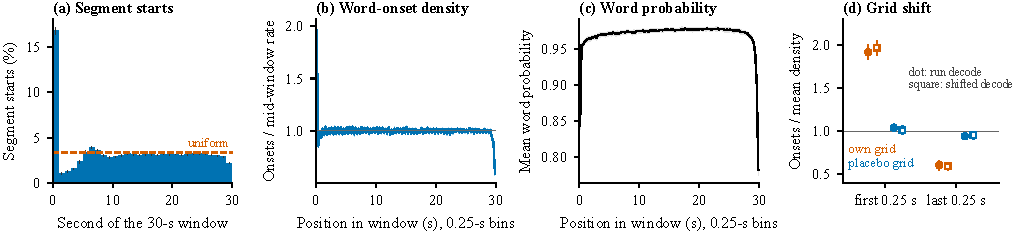
\includegraphics[width=\textwidth]{floats/fig_seams.pdf}
\caption{The fixed 30-s decoding grid marks the transcripts. \CapSeams{} Filter off in (a) to (c). In (d) each decode
is read on its own grid and on the other grid (placebo); dot: run decode, square: shifted decode. No audio was played.}
\label{fig:seams}
\end{figure*}

\SegStartSecZeroPct\% of segments start in a window's first second (uniform: \UniformSecondPct\% per second;
Figure~\ref{fig:seams}). Word onsets in the first 0.25\,s are \OnsetFirstQuarter{} times the mid-window rate, at word
probability \WordProbFirstQuarter; in the last 0.25\,s, \OnsetLastQuarter{} times, at \WordProbLastQuarter. Word times
are the recognizer's, not forced-aligned: \ZeroGapPct\% of within-segment gaps
are zero, and \PauseAtBoundaryPct\% of pauses of 0.3\,s or more sit at segment boundaries. The grid makes
\GridPauseSurplusPct\% of gaps of 0.3 to 30\,s (gaps pooled; 90\% \GridPauseSurplusLo--\GridPauseSurplusHi), \GridPauseTimePct\% of pause time, and
\GridFillerLastThreePct\% of filled pauses in a window's last 3\,s above the flat rate (90\%
\GridFillerLastThreeLo--\GridFillerLastThreeHi).

\paragraph{Grid shift.} \GsRecordings{} seen recordings, one per creator, were decoded again on a grid moved by 15\,s.
Decoding is deterministic: all \GsControlIdentical{} re-decodes on the run grid reproduce the record. The shift changes
\GsChangedPct\% of words (\GsChangedLo--\GsChangedHi; worker versions do not inflate this, Appendix~\ref{app:measure}).
\GsEditsNearRunSeamPct\% of edits lie within 1\,s of a run-grid seam, about \GsNearSeamRatio{} times the uniform
\GsUniformNearSeamPct\%, though most lie elsewhere. In a negative control \cite{lipsitch2010negative}, onset density in
a window's first 0.25\,s is \GsOnsetFirstOwn{} times the mean on a decode's own grid but \GsOnsetFirstPlacebo{} on the
other grid (Figure~\ref{fig:seams}d): the shift separates seam effects on onsets and timing from the speech.

The pause share moves by \GsPauseShareSd{} between-creator SD (\GsPauseShareSdLo{} to \GsPauseShareSdHi) and word
counts by \GsWordsDiffPct\%. On average no pause measure moves by more than \GsPauseSdMax{} SD and no word measure by
more than \GsWordSdMax{} SD, filled pauses excepted (\GsFillerSd; \GsFillerSdLo{} to \GsFillerSdHi;
Table~\ref{tab:gridshift}); these are intervals, not equivalence tests, on a lenient yardstick for change within one
recording. As no word crosses its own seam, own seams fall in pauses more often than placebo seams
(\GsSeamInPauseOwnPct\% against \GsSeamInPausePlaceboPct\%), so the seam rule's assumption of gaps independent of grid
phase (Section~\ref{sec:pipeline}) fails in part. The rule keeps creators' rank order (rank correlation at least
\SeamRuleRankCorrMin), so pause results are within-model rankings, not levels; timing measures are whole-span rates,
and thanks-phrase counts are tied to one grid position.

\subsection{An apparently inserted phrase and the positional filter}
\label{sec:artefacts}

Whisper-family models write fluent phrases with no speech behind them, tied to non-speech audio or long non-vocal
stretches \cite{koenecke2024careless,baranski2025investigation}. Here a stand-alone two-word thanks phrase, a closing
courtesy, appears to be inserted at window ends. On the run grid it starts in a window's last 3\,s
\ThanksPerSpeechHour{} times per hour of detector speech (hours pooled; creator-equal \ThanksPerSpeechHourCreator; 90\%
\ThanksPerSpeechHourLo--\ThanksPerSpeechHourHi, resampling creators with the grid fixed). It sits in
\ThanksPerWindowPct\% of windows mostly covered by other speech, \ThanksPerWindowPartialPct\% of partly covered ones and
none without speech: the detector gates decoding, so a window without speech reaches the recognizer empty, unlike the
non-speech audio of the cited studies.

Two untested accounts compete: decoding of windows from which the detector removed non-speech, or spoken closings at
window ends. A grid-made phrase would follow the shifted window ends, a spoken one its audio time. Thanks segments
(before the filter) are fewer on the shifted grid (\GsThanksRunRate{} against \GsThanksShiftRate{} per speech hour),
but the change is not distinguishable from zero (\GsThanksSd{} SD; \GsThanksSdLo{} to \GsThanksSdHi), and of
\GsPrecisionRemoved{} removals sought on the shifted decode, fewer than 5 creators have one that recurs at the same
audio time (no share printed; privacy rule).

The positional rule removes \ThanksLateSegments{} of \ThanksStandalone{} stand-alone thanks segments in full windows;
closings in the last, partial window escape it. If spoken thanks phrases were spread evenly over window phase, their
rate in the other 3-s bins would bound its precision at \ThanksPrecisionPoint{} (at least \ThanksPrecisionLow{} at a
conservative 95\% bound). The isolated-segment and loop rules are weaker, and the loop rule may remove genuine
repetition such as chanting (Appendix~\ref{app:artefacts}).

\subsection{Time without speech, and what the run covers}
\label{sec:nonspeech}

The voice detector's non-speech is \NonSpeechPooledPct\% of seen audio, hours pooled
(\NonSpeechPooledLo--\NonSpeechPooledHi), \NonSpeechCreatorPct\% creator-equal (\NonSpeechCreatorLo--\NonSpeechCreatorHi)
and \NonSpeechMedianPct\% at the creator median, so creators with much of it pull the means up. Time outside recognizer
segments is \OutsideSegPooledPct\% pooled (\OutsideSegPooledLo--\OutsideSegPooledHi). Neither tells music, toning,
meditation and silence apart; long pauses count as non-speech.

Time outside segments gathers at the end (Figure~\ref{fig:coverage}, Appendix~\ref{app:measure}): segments cover \LastPartialCoverage{} of the
last, partial decoding window (\LastPartialCoverageLo--\LastPartialCoverageHi), against \WindowBeforeCoverage{} of the
window before and \MiddleCoverage{} in the middle of recordings of 6\,min or more. The dip mixes decoding, as the
partial window is short, with content, as the window before also drops when the partial window is short; without a
positional figure for the detector, the two cannot be separated.

\paragraph{Coverage by listing rank.}
\label{sec:coverage}
Within creators, a recording at listing ranks 1--5 is likelier than one at ranks 6--20 to lack a run transcript
(Mantel--Haenszel odds ratio \OrNotTranscribed; creator bootstrap \OrNotTranscribedLo--\OrNotTranscribedHi). Text set
aside drives this (\OrOtherText, \OrOtherTextLo--\OrOtherTextHi), much of it the project's own earlier recognizer text
(\NOwnEarlierAsr{} of \NSetAside{} set-aside recordings); having no text at all does not depend on rank (\OrNoText,
\OrNoTextLo--\OrNoTextHi). Rank is listing order, not time: run-transcript analyses under-represent the newest uploads,
and the caption anchor comes from those ranks.

\subsection{Variance structure and error tolerance}
\label{sec:variance}

On \VpCreators{} creators and \VpRecordings{} recordings, the intraclass correlation (ICC: share of variance between
creators, on a named scale) is \IccPace{} for pace (words per minute; \IccPaceLo--\IccPaceHi), \IccNonspeech{} for the
share without speech (logit; \IccNonspeechLo--\IccNonspeechHi), \IccContr{} for contractions (negative-binomial latent
scale; \IccContrLo--\IccContrHi), \IccMattr{} for MATTR-500, a moving-average type-token ratio
(\IccMattrLo--\IccMattrHi), \IccRepFive{} for the repeated five-word share (logit; \IccRepFiveLo--\IccRepFiveHi) and
\IccSegLogp{} for mean segment log-probability (nats; \IccSegLogpLo--\IccSegLogpHi; Table~\ref{tab:vp}); for counts the
ICC depends on the scale \cite{nakagawa2017coefficient}. Between-creator variance holds channel and recognizer variance
as well as the speaker's. For pace the Kish design effect (variance inflation from clustering) is \KishPace{} (about
\NeffPace{} effective recordings), and a ten-recording creator mean has reliability \RtenPace: inference must be at the
creator level.

Error injected uniformly with the bridge's edit profile, as in word-error simulations
\cite{proksch2019testing,fetic2021topic}, moves cohort means of pronoun, contraction and question-mark rates by under
0.2 between-creator SD up to 20\%. Word length, MATTR-1000 and filled pauses reach 0.2 SD at about \TolWordLenPct\%,
\TolMattrPct\% and \TolFillerPct\% (Table~\ref{tab:tolerance}), at or just above the measured disagreement (bridge
median pair \BridgeDisagreeMedianPct\%; captions \AnchorCaptionMeanPct\%, blind to fillers). The 90th-percentile
creator crosses earlier, below the bridge's median-pair disagreement for filled pauses and MATTR-1000, and uniform
injection understates systematic loss of fillers and contractions, so between-creator comparisons of these three
measures are not supported for creators in the upper tail. At a median error of 10\%, error that differs between
creators and tracks the share without speech can move their correlation with that share by up to \RSixAssocMax{}
(\RSixFillerAssoc{} for filled pauses). Tolerance, not accuracy.

% sections/protocol.tex -- Section 6, the registered protocol for model-coded labels.
% Writer: C. Written 2026-11-21, 06:07 to 06:25 UTC; second review round 08:04 to 08:40 UTC; third review round from
%   11:50 UTC (clock: date -u): A10 drafted, not entered, and the amendment count (methods review M14, privacy P8); the
%   reporting plan's registration time and what came before it (M13); the title gates of record on G and the revision
%   count of each instrument (M19, P11); the known-answer battery on revision 3 (registry 09:10); the interfaces and the
%   hard stop at worst case (registry 04:55 to 11:10). Moved to Appendix B by the page limit: tab:status and
%   tab:status-labels, the second-reading detail, part of the cross-vendor paragraph and Section 6.7 (move log, private
%   fix list).
% Fourth review round from 12:35 UTC (clock: date -u): the merge reaches H1 and H6 (methods review M12); the choices
%   after a gate result and freeze 1's timing (M6); the known-answer bounds stated with their assumption (M3); what
%   weakens VG-6, the middle model's row and the 03:21 release rule (M5, M11). New macros: \VtrOtherClaimedSharePct,
%   \VtrSealMadeStamp (and \VtrMiddleRunOne, already built).
% Macros used that are not in outline section 7: \DblSUnits, \DblFcUnits (requested in findings/macros-requested-C.md),
%   and the third round's \KaKoneRSmallRevThree*, \KaKfourVSmallRevThree, \KaCvSixSmallRevThree, \KaSpillRRevThree*,
%   \KaMiddleRevThree*, \TitlePresKappaG*, \TitlePresFloor, \PlanRegisteredStamp, \ProdSeen*, \ProdCommittedUsd.
% Citations: pangakis2024keeping, teblunthuis2023misclassification, vandenakker2021preregistration,
%   vanmiltenburg2021preregistering, anderson2017splitsample, fafchamps2017using, egami2022make (refs.bib).
% Results round (2026-11-21, from 19:16 UTC; clock: date -u): the registry rows after 13:05 and its sections 'Freeze 1,
%   amendment 1' and 'Freeze 2': A10 entered (16:07), freeze 1 written again (16:06) and freeze 2 (16:10) with its
%   constants, hold-out production, R-hold and the checkability check on the hold-out, the plan-mode limit of the
%   reliability driver, interfaces and the hard stop at worst case, the final spend and what was not bought (HR).
%   New macros: \FreezeOneAmendStamp, \FreezeTwoShort, \FreezeTwoPrefix, \FreezeTwoModules, \ConstantsStamp,
%   \HFourYardstick*, \HFourMinForms, \HTwoBandLo, \HTwoBandHi, \HNineSesoi, \ATenStamp, \ATenShaPrefix,
%   \HoldoutProd*, \Rhold*, \ChkHoldout*, \HardStopRefusal*, \LabellingDoneStamp, \Final*, \HrAUsd.
% Pending labels used: \PendVerDep.
% Pre-publish verification (2026-11-21, from 21:30 UTC; clock: date -u): Table tab:gates covers the gate sample G; the
%   gate failures on R-hold (forecast class D, sentence codes C) from the public results file (\ResRholdGates).
% "registry 03:08" and the like name rows of the registry dated 21 November 2026 (UTC); times are commit times
%   (registry 06:44 (10)).

\section{The registered protocol for model-coded labels}
\label{sec:protocol}

No person checked any label (amendment A8), so neither the labels' accuracy nor a correction for misclassification can
be estimated \cite{pangakis2024keeping,teblunthuis2023misclassification}. Tables~\ref{tab:status}
and~\ref{tab:status-labels} (Appendix~\ref{app:protocol}) give each construct's status and allowed uses.

\subsection{Registry, hold-out and freezes}
\label{sec:registry}

The registry of analyses on data already collected
\cite{vandenakker2021preregistration,vanmiltenburg2021preregistering} was frozen at \RegistryFrozenStamp{} (commit;
SHA-256 prefix of the hypotheses file \HypothesesShaPrefix): H1 to H10 under Holm correction and the exploratory
questions E1 to E13. H3 alone needed no labels; it was frozen at \HThreeFrozenStamp{} and run at \HThreeRunStamp{}
(Section~\ref{sec:hthree}). Only internal commits attest the freeze; an external registration is the owner's act.

\label{sec:holdout}
The hold-out, a split sample of whole speakers \cite{anderson2017splitsample,fafchamps2017using,egami2022make}, is the
\NHoldout{} creators with at most three of the first \SnapLines{} finished transcripts and ten or more still to come:
the tail of an English-first run queue (from \EnglishFirstStamp), holding all \NNonEnglishCreators{} creators with a
non-English transcript. Fields known before the run separate it from the seen creators (cross-validated AUC \DTwoAuc{} on
\DTwoFields{} fields; 95\% shuffle band \DTwoAucBandLo--\DTwoAucBandHi; Figure~\ref{fig:love}, Table~\ref{tab:balance}),
so hold-out-only estimates are primary and seen against hold-out is never read as replication. Contacts:
Table~\ref{tab:contacts}.

\label{sec:freezes}
Freeze 1, recorded at \FreezeOneStamp, hashes \FreezeOneFiles{} instrument files and the configuration (prefix
\FreezeOneConfigPrefix): models (small \ModelSmall, middle \ModelMiddle, large \ModelLarge), the record model per
instrument and group (middle for hold-out voice), efforts and output caps (Table~\ref{tab:freeze}). It unlocked
seen-creator production only (\ProdSeenStamp). It was written again at \FreezeOneAmendStamp{} for the production
driver alone, which gained a feature step for the other groups that runs after freeze 2 with the frozen feature code
(registry 15:14). Freeze 2 (\FreezeTwoShort; record prefix \FreezeTwoPrefix) hashes \FreezeTwoModules{} analysis
modules and the constants, computed on seen labels alone, names the registry commit that holds A10, and unlocked the
hold-out labels and the tests. H4's yardstick keeps a minimum of own-voice forms set before any seen label, as a stated
choice; H9's smallest effect is the placeholder, \HNineSesoi, adopted rather than set from seen cells (16:06; a
deviation; constants in Appendix~\ref{app:protocol}).

\paragraph{First-round production.} Hold-out labels (\HoldoutProdRecordings{} English recordings,
\HoldoutProdStamp), R-hold's reliability runs and a large-model reread of hold-out statements followed under both
freezes (interfaces, the hard stop's one refusal and the reliability driver's plan-mode limit in
Appendix~\ref{app:protocol}). Labelling ended at \LabellingDoneStamp{} with \FinalCommitted{} USD committed, past the
owner's 120 USD warning and \FinalBelowStop{} below the hard stop; HR (a) and HR (b, c) were not bought.

\subsection{Amendments}
\label{sec:amendments}

\NAmendments{} amendments are entered (A1 to A11). A1 to A4 came with the freeze and the rest after
H3's result (Section~\ref{sec:deviations}). A9 drops H8 ($p = 1$). A11 replaces the human check by verification with
models; every rule that named a person got a named substitute, and no floor was lowered (registry 03:08), though the
release rule of the hold-out robustness rows was loosened at 03:21 (Section~\ref{sec:verification}). A10's text,
decided at 03:08 and worded after freeze 1 without using any label, was entered at \ATenStamp, before freeze 2 and any
hold-out label, from the draft whose hash it records (prefix \ATenShaPrefix): creator-level sign-flip $p$ in Holm ($m = 10$; unrun at $p = 1$), ``not determinable: too few eligible
creators'', conditional H5 and H6 estimators, the combined gate rule, H7's estimator, and $t$ intervals on creator means
with HKSJ pooling. Where A10 replaces a registered estimator, reference, minimum, interval or
centring, both versions are computed, the larger $p$ enters Holm, and a verdict stands only if both give it; other
changes, such as the M9 revisions of H2 and H5, are outside the guard (registry 06:44 (7)). A result is
\emph{uninformative} when its 90\% creator interval holds zero and the smallest effect of interest in either direction,
or its verdict is not determinable. The exploratory reporting plan (prefix \PlanShaPrefix) was registered by hash at
\PlanRegisteredStamp, after most of the outputs it governs had been built, as its addendum 1 (\AddendumOneStamp) states,
naming them; it reports every listed output whatever it shows.

\subsection{Instruments and gates}
\label{sec:instruments}

The instruments (voice, asks, forecast critic, checkability, commitment, sentence codes, titles) face gates A to E:
valid answers, exact quotations, three-run stability, two-model agreement, agreement with a second finder. A gate
passes when the point estimate reaches its floor and the lower 90\% bound the floor minus 0.10. Voice, asks and the
forecast critic each spent the one revision that the annotation plan (section 3.4) allows; after it, an instrument takes
one of the merges declared there in advance (Appendix~\ref{app:protocol}) or is not frozen, and the hypotheses that need
it are ``not run for want of an instrument'' ($p = 1$; A10.5). A10.5 writes one exception into the rule: the owner's
decisions of about 00:30 keeping checkability (H2) and the title codes (H5, H9), which had failed gate D after both
pilot revisions, stand, with their failed gates reported, and extend to no other instrument. Table~\ref{tab:gates} lists
every gate on the gate sample G, failures included. \ResRholdGates

Voice revision 3 passes gates C (\VoiceGateC{} against \VoiceGateCFloor) and D (claimed, own and other voice,
\VoiceGateDKappa). Its relayed-voice row fails (\VoiceRelayedKappa{} [\VoiceRelayedLower]), and the pre-declared merge,
frame-only relay reported apart, does worse (\VoiceFrameOnlyKappa{} [\VoiceFrameOnlyLower]); by the letter of the rule,
H1, H4 and H6 would then be not run. At 02:55, after these results and under the owner's delegation, relayed voice was
merged into claimed voice instead, the voice that H1 and H6 use (H4's primary stays embodied voice, the merged voice a
secondary row; registry 04:55 (a)), and relayed-only rows carry no verdict; Table~\ref{tab:deviations} classes this
merge as looser. Two further choices followed a gate result: the ask check's record moved to the middle model after the
small model's check failed gate B (02:20), and the forecast critic's class of record became F1 against the rest after
the ten-class label failed gate C (03:12; looser for the gate). Freeze 1 did not wait for the known-answer voice
batches, against the 03:08 rule that it wait for the battery (04:59; looser for its timing). The label moves more
without punctuation and case than between runs (\VoicePunctMovePct\% against \VoiceRunMovePct\% of words), and every
voice result says so. Checkability and title presentation (gate D \TitlePresKappaG{} against \TitlePresFloor; figures
in Appendix~\ref{app:protocol}) are kept below their floors by the owner's exception, with large-model adjudication. A
verdict of H2, H5 or H9 therefore rests on an instrument below its floor and carries that flag
(Section~\ref{sec:results}).

\subsection{Verification}
\label{sec:verification}

If constructed texts are easier than speech (not tested), recovery shares on them are upper bounds for the corpus and
error shares (spill, non-asks kept) lower bounds; the levels are printed, but only differences between cells are
interpreted (Table~\ref{tab:ka}). On voice revision 3, the frozen form, the small model recovers
\KaKoneRSmallRevThree{} of planted relayed passages (90\% \KaKoneRSmallRevThreeLo--\KaKoneRSmallRevThreeHi;
\KaKoneRSmall{} on revision 2); the middle model, the hold-out record, stays at \KaMiddleRevThreeLo{} to
\KaMiddleRevThreeHi{} on the voice arms (registry 09:10; the other arms, the canary gates, the void arms and a second
reading by another model of the same vendor, whose time-window disagreements gave H2 a sensitivity row, in
Appendix~\ref{app:protocol}).

Gate VG-6, its meaning fixed at 03:21 before its seal was opened, passes (Table~\ref{tab:crossvendor}): model-coded; a
model of another vendor (Anthropic), reading blind with ten units of context on each side, agreed with the OpenAI
readers' majority on claimed, own and other voice with kappa \VtrKappa{} (90\% creator bootstrap \VtrKappaLo{} to
\VtrKappaHi, weighted to the frame; \VtrUnits{} units of \VtrCreators{} creators, unweighted \VtrKappaUnweighted;
strata and weights in Appendix~\ref{app:protocol}); not checked by a person. It is a weaker check than it looks: the
majority it is compared with is the small model's three runs and the middle model's first run; the reader is of the
model family that made the lead's decisions and drafted this paper; about \VtrOtherClaimedSharePct\% of the weighted
disagreement is the reader's ``other'' where the majority says ``claimed'', the voice that H1 and H6 use and of which
H4's embodied voice is part; and the sealed figures were computed at \VtrSealMadeStamp, before the 03:21 row fixed the
meaning of pass and fail, though opened only after freeze 1. The effective number of readers is pending (\PendVerDep).
Against the middle model's first run, the hold-out record, kappa is \VtrMiddleRunOne. With the known-answer gates it met the release rule of the hold-out robustness rows, loosened at 03:21 for the
model fallback; the rows were not bought.

% sections/tests.tex -- Section 7, first-round tests: design, projections and power stated in advance.
% Writer: C. Written 2026-11-21, 06:09 to 06:25 UTC; second review round 08:04 to 08:40 UTC; third review round from
%   11:55 UTC (clock: date -u): power at the nearest CAL count (methods review M20); H5 and H2 not announced, H9 not
%   projected (P12, P13); the registered H3 row (P14, M24); the plasmode's conditioning (M24); the hypothesis-code
%   decisions of 06:44, 09:19 and 11:08 (registry). Moved to Appendix B by the page limit: tab:programme and the H3
%   detail (t interval from the published summary, recentred value, calibration, power, coverage).
% Fourth review round from 12:40 UTC (clock: date -u): the count of hold-out creators with English recordings is not
%   printed (privacy review P5: beside the hold-out and non-English counts it gives a cell of fewer than 5 by
%   difference); "as registered and amended" (M12).
% Macros used that are not in outline section 7: the third round's \HThreeRegLo, \HThreeRegHi, \HThreeShiftP,
%   \HSixSignFlipRejectPct, \HSixBurstRejectPct, \HSixBurstSize, \HSixDraws, \PowerHTwoCreators, \PowerHFiveCreators.
% Results round (2026-11-21, from 19:16 UTC; clock: date -u): H9's smallest effect adopted at the placeholder (16:06);
%   CAL part (f) not run, the battery in its place (15:14 (2), 16:06 (2)); the last code decisions before freeze 2 in
%   one sentence (12:52); Section 7.3 reads the public results file through findings/results.tex (\Res... macros),
%   written for every outcome (supported, refuted, not determined, not determinable, uninformative); tab:results.
% Pending labels used: \PendHThreeX; the result macros of findings/results.tex expand to \pending{...} until the public
%   results file exists.
% Pre-publish verification (2026-11-21, from 21:30 UTC; clock: date -u): the recording-property projections are stated
%   against the minimum only (\ProjH...Rec are text, e.g. "more than 12"; the projections are capped at a withheld
%   count); the gate failures on R-hold from the public results file (\ResRholdShort, findings/results.tex).
% Citations: card2020little, lipsitch2010negative, cameron2008bootstrapbased, mackinnon2022clusterrobust (refs.bib).
% "registry 02:50" and the like name rows of the registry dated 21 November 2026 (UTC).

\section{First-round tests}
\label{sec:tests}

An exact creator sign-flip passes the first Holm step (0.005) only from \MinCreatorsOneSided{} creators one-sided or
\MinCreatorsTwoSided{} two-sided, which amendment A10 makes H2's minimum; the registered minimum for H1 and H4 to H6 is
\MinCreatorsRegistered{} (programme: Table~\ref{tab:programme}).

\paragraph{Announced in advance.} Before any hold-out label (registry 02:50), with power stated before results
\cite{card2020little}, H1, H4 and H6 were announced as probably not determinable. CAL projects eligibility from
model-coded pilot labels as a property of the creator or of each recording (Figure~\ref{fig:eligibility}; ranges and
smallest attainable $p$ in Table~\ref{tab:programme}). The announcement rests on the first, lower bound, \ProjHOne,
\ProjHFour{} and \ProjHSix{} eligible creators against \MinCreatorsRegistered, where no $p$ can pass the first Holm
step; the second puts all three above the minimum (\ProjHOneRec, \ProjHFourRec{} and \ProjHSixRec{} creators at the
median), with CAL power \PowerHOneUpper, \PowerHFourUpper{} and \PowerHSixUpper{} at
\PowerUpperCreators{} creators. The pilot cannot tell the bounds apart (the first holds if eligibility is a fixed habit
of the creator, the second if it varies by recording), so the announcement is a statement of risk on the cautious
bound, not a forecast. Not announced: H2 (\ProjHTwo{} or \ProjHTwoRec{} creators; power \PowerHTwo{} at $|D| = 0.10$)
and H5 (\ProjHFive, an upper bound; power \PowerHFive). H9 is not projected (its cells need labels and the name list);
its smallest effect is the registry's placeholder, \HNineSesoi{} standardised units (16:06). H2, H5 and H9 rest on
instruments below their floors (Section~\ref{sec:instruments})\ResRholdShort.

\paragraph{Calibration and revisions.} Under a creator-level placebo \cite{lipsitch2010negative}, H2's registered
within-creator reference rejects about \HTwoRefTimesNominal{} times nominally and H6's half-count rule \HSixRefTimesLo{}
to \HSixRefTimesHi{} times; A10 replaces them under its guard. CAL's repeat on seen labels (part f) did not run; the
simulation battery stands in for it (16:06). Other findings and every code revision before freeze 2 (the last at 12:52)
are in Appendix~\ref{app:protocol}.

\subsection{H3, restated}
\label{sec:hthree}

H3's registered row is $U$ = \HThreeU{} on \HThreeCreators{} hold-out creators (90\% \HThreeRegLo{} to \HThreeRegHi;
shift $p$ \HThreeShiftP). Restated (registry 03:08; Table~\ref{tab:hthree}): supported by its registered rule, which
says ``supported'' under placebo in \HThreePlaceboSeventeen\% of sets of \HThreeCreators{} creators against 0.5\%; not
determined at the creator level; exploratory; withdrawn (A6); its wave replication was not run, and creator-level rows
on the hold-out wait for H3-X (\PendHThreeX).

\subsection{Results}
\label{sec:results}

\ResSummary{} \ResCounts{} \ResHolm{} Table~\ref{tab:results} gives each result, Appendix~\ref{app:protocol} both
versions, the robustness rows and the Holm table. Labels are model-coded (A8); a supported or refuted
verdict reads ``verified by a third model, on known-answer texts and by a reader of another vendor''; uninformative
results leave the headline claims, their rows kept (A2). \ResDiscussion{} A replication wave, which H7 and H10 need,
would show persistence, not confirmation (Figure~\ref{fig:plasmode}).

\begin{table}[t]
\centering
\small
% tab_results.tex: GENERATED by WORK/build_numbers.py at 2026-11-22T01:51:42Z; label tab:results. The writer adds the float,
% the caption and the label. Sources: REG/results/first-round-2026-11-21.json
% Eligible: creators of the amended (primary) version / its minimum; $<$5, $<$min., $\geq$min.: a count stated against 5 or against the minimum only. Estimate on its natural scale with its 90\% creator interval. Holm-adjusted $p$ of the larger of the two versions' $p$. $\dagger$: instrument below its floor (owner's exception, A10.5).
{\scriptsize\setlength{\tabcolsep}{2pt}
\begin{tabular}{@{}p{0.05\linewidth}p{0.16\linewidth}p{0.30\linewidth}p{0.09\linewidth}p{0.23\linewidth}l@{}}
\toprule
 & Eligible & Estimate [90\%] & Adj.\ $p$ & Verdict & Uninf. \\
\midrule
H1 & $<$min. / 12 & n.p. & 1 & not determinable & yes \\
H2$^{\dagger}$ & $\geq$min. / 9 & n.p. & 1 & not run for want of an instrument & yes \\
H4 & $<$min. / 12 & n.p. & 1 & not determinable & yes \\
H5$^{\dagger}$ & $<$min. / 12 & n.p. & 1 & not determinable & yes \\
H6 & $<$min. / 12 & n.p. & 1 & not determinable & yes \\
H9$^{\dagger}$ & $<$5 / 8 & n.p. & 1 & not determinable & yes \\
\bottomrule
\end{tabular}}

\caption{First-round results on the hold-out (public results file; model-coded): eligible creators of the primary
version / its minimum ($<$5, $<$min., $\geq$min.: a count stated against 5 or the minimum only); estimate with its 90\%
creator interval (n.p.: not printed); Holm-adjusted $p$ of the larger of the two versions' $p$; verdict under A10's
guard; uninformative flag. $\dagger$: instrument below its floor. \ResPendingNote}
\label{tab:results}
\end{table}

% sections/deviations.tex -- Section 8, deviations from the registered design.
% Writer: C. Written 2026-11-21, 06:12 to 06:14 UTC; second review round 08:20 UTC; third review round from 12:00 UTC
%   (clock: date -u): A10 as drafted; the registry rows after the A10 draft's last alignment (09:19, 11:08, 11:10) and
%   the A10 rows of contacts, the freeze-1 entry and corrections of the record now enter once each (builder);
%   condensed for the page limit (the decisive deviations are each stated where they occur, Sections 6 and 7).
% Fourth review round from 12:40 UTC (clock: date -u): A10's guard stated as what it covers, the looser and mixed
%   rows named as outside it (methods review M1); the class 'mixed' for rows stricter for some uses and looser for
%   others, and for the M9 revisions (M11; registry 06:44 (7)).
% Macros used that are not in outline section 7: \NDevStricter, \NDevGuarded, \NDevNeutral, \NDevLooser, \NDevMixed,
%   \NDevExploratory, \NDevBudget, \NDevOther (they sum to \NDeviationRows), \SpendMeasured, \SpendCommitted,
%   \SpendStamp.
% Results round (2026-11-21, from 19:16 UTC; clock: date -u): the deviation table reads the registry's own table (A10
%   Part 8, entered 16:07) and the registry rows after it (16:06 to 23:34 since the final pre-push check); H9's
%   smallest effect (16:06) is a mixed row; HR not bought (16:26, 18:17, 18:41); the final spend, past the warning.
% Final pre-push check (2026-11-21, from 23:35 UTC; clock: date -u): the simulation battery (21:52) is a budget or
%   operations row; the rows of the public results file (20:48, 22:33, 23:34) are reporting, counted in \NDevOther,
%   whose definition (disclosure, correction of the record, the freeze-1 entry, reporting, not yet decided) is in the
%   table's caption; the
%   exploratory round's start (23:17) is an exploratory row.
% Pending labels used: none. Sources: D6-deviation-table.csv, the deviation part of the A10 draft, registry rows after
%   it, llm/spend.jsonl (read-only).

\section{Deviations from the registered design}
\label{sec:deviations}

Table~\ref{tab:deviations} lists \NDeviationRows{} deviations from the frozen registry, each with its time, decider,
the results known then and its direction: \NDevStricter{} stricter, \NDevGuarded{} guarded by A10, \NDevNeutral{}
neutral, \NDevLooser{} looser, \NDevMixed{} mixed (of more than one or of an unknown direction, outside the guard),
\NDevExploratory{} exploratory, \NDevBudget{} budget or operations and \NDevOther{} other (timeline in
Figure~\ref{fig:timeline}).
Decisive: H3's reference held creators fixed, its estimand was off-centre and its interval unaudited, and it was closed
(A6) without its wave replication; the selection rule was written after H3's test. Changes of estimator, reference,
minimum, interval or centring fall under A10's guard; the looser and mixed deviations do not, among them the merge of
relayed into claimed voice after its gate and the pre-declared merge had failed, the forecast critic's class of record,
the instruments kept below their floors, freeze 1's timing, the release rule of the hold-out robustness rows, and the
M9 revisions of H2 and H5, which the registry keeps outside the guard (06:44 (7)) and reports beside the rows without
them, and H9's smallest effect, the registry's placeholder adopted rather than set from seen creators (16:06). The
round cap of 50 USD was exceeded
through the channeler discovery (registry 03:08); total OpenAI spend was \SpendMeasured{} USD measured and
\SpendCommitted{} USD committed at \SpendStamp, past the 120 USD warning and under the 130 USD hard stop.

% sections/limitations.tex -- Section 9, limitations (outline section 5, sec:limits).
% Writer: A. Written 2026-11-21, 06:15 to 06:50 UTC; second review round 08:22 UTC; third review round from 12:02 UTC
%   (clock: date -u): the review conditions still unmet and the canonical literature not cited (methods review M17);
%   the caption row's representativeness and normaliser (M16); the small voice model on revision 3 (registry 09:10;
%   P24); A10 as drafted (P8); condensed for the page limit (every contact keeps its UTC time; the instrument details
%   stand in Sections 6 and 7).
% Fourth round from 12:45 UTC (clock: date -u): the known-answer bound with its assumption (methods review M3); the
%   thanks count "may depend" on the grid (M2); the HR release rule and the class of record (M6, M11).
% Macros used that are not in outline section 7: \NCloudOnlyObjects (requested in findings/macros-requested-A.md).
% Results round (2026-11-21, from 19:16 UTC; clock: date -u): A10 entered; hold-out text sent to the API after freeze 2;
%   HR not bought; the anchor against possibly human-made texts allowed after freeze 2 and still pending.
% Pre-publish verification (2026-11-21, from 21:30 UTC; clock: date -u): the R-hold gate failures (\ResRholdShort).
% Pending labels used: none.

\section{Limitations}
\label{sec:limits}

\paragraph{Selection.} The roster is a judgment sample: its rule was written down late, it grew on the day of the listing, and a discovery harvest closed early (Section~\ref{sec:data}). Intervals refer to creators like these; live streams, short videos, paid material, other platforms and deleted recordings are missing; nothing describes mediums at large, a period or a trend.

\paragraph{No human reference.} No text known to be made by people exists for the seen creators, so no word error rate is measured; agreement with automatic captions is not accuracy, rests on \AnchorCaptionRecordings{} set-aside recordings and uses a normaliser chosen after the result. No detector decision, language decision, artefact rule or label was checked by a person (A8); agreement between models is reliability, not validity; known-answer recovery bounds corpus recovery from above only if constructed texts are easier than speech, which was not tested; errors that all model readers share go undetected.

\paragraph{Recognizer, voice and languages.} The 30-s grid leaves seams, and the count of a thanks phrase that appears to be inserted, and any measure built on it, may depend on where the grid sits. Time stamps are the recognizer's; timing measures are used inside one model only; non-speech is the voice detector's, which also gates decoding; \LangCreatorRulePct\% of language decisions rest on the creator rule. Voice spans are inferred from text without speaker separation, and the own voice concentrates in openings and closings, so voice is partly confounded with position. Without a corpus of non-channelling speech, nothing is called distinctive of channelling. Every other language has fewer than five creators, all in the hold-out; the bridge covers English only.

\paragraph{Hold-out.} The \NHoldout{} hold-out creators are the tail of an English-first run. Before freeze 2, hold-out material was touched (Table~\ref{tab:contacts}) by the first panel's tables (\ContactSnapshotFiles{} files, \ContactSnapshotStamp) and position pilot (\PilotCreators{} creators, time not recorded), the run report's position displays (\ContactRunReportStamp), H3's run (\HThreeRunStamp), a panel script that loaded about \ContactCoverageFiles{} metadata files (\ContactCoverageStamp), TABLE's logged extraction (\ContactTableStamp), the public-output generators that loaded the run report's per-recording timing cache (\ContactPrivacyStamp), and the one-off script that cut that cache to the seen creators (\ContactSeenDerivStamp). None produced a statistic of a registered hypothesis on hold-out text other than H3's test, and this paper prints no number from them. After freeze 2, hold-out transcript windows went to the OpenAI API for the frozen instruments only (ethics statement).

\paragraph{Programme and instruments.} H3 passed a rule not calibrated at the creator level and was withdrawn; H1, H4 and H6 fall below their minimum on the lower of two projections that the pilot cannot tell apart. H2, H5 and H9 rest on instruments kept below their floors by the owner's exception\ResRholdShort; relayed voice was merged after its gate failed; the release rule of the hold-out robustness rows was loosened, and those rows, the rewording rows among them, were not bought; the forecast critic's class of record was chosen after its ten-class label failed; H9's smallest effect is a placeholder adopted without a rule; the recorded gates used another large model than production; on the frozen voice form the small model trails the middle one on some known-answer arms (Table~\ref{tab:ka}); entrance cues were read once by a model.

\paragraph{What the review asked for and is not met.} The paper review asked for an external reference (none exists for the seen creators; the anchor against possibly human-made texts of other creators is pending), an ethics determination (none exists; the paper is not to be submitted before it) and the canonical literature on channelling and its milieu (not cited: no verified entries exist in this draft). The corpus cannot be shared, so the results cannot be reproduced elsewhere.

% sections/conclusion.tex -- Section 9, conclusion (label sec:conclusion). Complete rewrite of 2026-11-21 (PaperOrchestra-
%   style section writer; clock: date -u 22:59 UTC), from outline.json (section_plan; attack_response PRES-1, SIG-1, CLAIM-2,
%   LINK-1). Recommendations drawn from existing results only; no new number. \ResConclusion comes from findings/results.tex.
% Integrator's page cut (2026-11-21): the two lists of recommendations kept, each in one sentence (outline cut 3, in
%   part); Sections 4.2 to 4.5 and 7 give each in full.
% Pending macros used: none.

\section{Conclusion}
\label{sec:conclusion}

Counts and labels of online spiritual speech need an audited pipeline first. Without human text, studies of fixed-window transcripts can report an anchor ladder instead of a word error rate, re-decode a sample on shifted and placebo grids before trusting timing, filter window-end phrases by position with the rule's assumption stated, treat the creator as the unit, and check word measures against the measured machine disagreement. Registered studies with model-coded labels can project eligibility on the cautious bound, re-gate instruments on a hold-out reliability sample, report labeller dependence and deposit the registry externally. \ResConclusion{} The paper reports no finding about channelling.

% sections/ethics.tex -- Ethics statement, unnumbered, before the references (label sec:ethics). Complete rewrite of
%   2026-11-21 (PaperOrchestra-style section writer; clock: date -u 22:59 UTC), from outline.json (section_plan; attack_response
%   ETH-1, ETH-2, ACC-1, HARM-1, FLOW-1, PROP-1, REPRO-1) and raw_materials (experimental_log sections 19 and 22).
% Integrator's page cut (2026-11-21): the writer's cut (c) in part (storage named once, without its places); the lead's
%   delegation, defined in Section 1, not restated. Paragraph names are unchanged (the checklist, Appendix D since 2026-11-26, cites them by name).
% \label{sec:ethics} sits on an unnumbered section: refer to it by name ("the ethics statement"), not by \ref.
% The checklist (Appendix D) points to the paragraph "Risks and misuse" by that name. Ledger figures: one read of the request ledger
%   (findings/numbers.tex); "30 days" is the vendor's documented term, not a measured number. Pending macros used: none.

\section*{Ethics statement}
\label{sec:ethics}

\paragraph{People in the data.} The creators are public communicators; their recordings also carry the speech of guests, clients and audience members (\ThirdPartySharePct\% of words in a model-coded pilot; 95\% \ThirdPartyShareLo--\ThirdPartyShareHi), with religious belief and possibly health matters. Public availability is not consent, and no consent was sought; copies are held privately for non-consumptive analysis.

\paragraph{Risks and misuse.} Besides re-identification (below), a minority spiritual practice may be stigmatised, and the instruments for asks and forecast checkability, with the planned test of later silence about passed dates, could serve to debunk or target creators and their clients. Hence no label, instrument output or per-creator value is released; claims get no truth label, nothing is said about sincerity, health or mental state, and asks are coded for placement, not intent.

\paragraph{Protections and their limit.} The paper holds no transcript text, quotation, name, code, identifier or title, no row for one recording or creator, no cell under five creators and no hold-out label count; timing displays use seen creators only. These rules cover this paper only: public project records outside it name the channels and list their recordings, and their history holds earlier per-recording files, so linkage could identify the creators behind aggregate counts; restricting them is the owner's act, not yet done.

\paragraph{External processing.} The \ExtRequests{} OpenAI API requests included about \ExtWordsM{} million words of transcript-derived text with repeats (an estimate): text of seen creators and, after the analysis freeze, of hold-out and other-group creators for the frozen instruments only. Requests carried \texttt{store=false}, but the vendor keeps abuse-monitoring logs for up to 30 days, and no zero-retention approval is on file. Seen statements went to the vendor's web-search tool in \ExtWebStatementRequests{} requests, which may have reached outside search providers (not assessed). The Anthropic agents' requests were not logged and their retention terms not read; stored copies have no decided retention period or deletion route, and uploads their creators later delete are not yet handled (Table~\ref{tab:external}).

\paragraph{Not yet in place.} None of these exists: an ethics or exemption determination; a lawful basis for archiving the audio and for sending participants' speech to a commercial service; a data-protection assessment, so the proportionality of external labelling was not assessed; a removal route. Platform terms and model licences are not covered, and a rule keeping client and audience spans out of future calls awaits the owner's decision.

\paragraph{Agents, accountability and reproducibility.} Anthropic model agents did the panels, hypothesis proposals and review, the first panel's transcript reading, the literature work, the cross-vendor reading, the lead's decisions and the drafting; records name vendor and role, not a model version per step. No person read or listened to the processed material or checked a label, and the registry records no review of the lead's decisions by a person.


\bibliography{refs,refs-new}

\appendix
% Each appendix flushes its floats before the next one starts, so that every float stays in its own appendix.
\clearpage
% sections/appendix-measurement.tex -- Appendix A, measurement records.
% Writer: B. Written 2026-11-21, from 06:19 UTC (clock: date -u); end time in fix-list-B.md.
% Word count: not budgeted (appendix); one or two sentences per float plus captions.
% Macros used that are not in outline section 7: none.
% Pending labels used: \PendSegLogpTwoLevel.
% Floats placed here (23; tables have bodies floats/<file>.tex holding the tabular only, caption and label here, except
%   tab:exclusions, whose tabular is written below because the outline gives it to writer B):
%   tab:wer-strata, tab:gridshift, tab:headlines (table*), tab:drift, fig:rank, tab:rank-odds, fig:love, tab:balance
%   (table*), fig:classes, tab:nonspeech, tab:vp (table*), fig:tolerance, tab:tolerance, tab:bridge-verdicts, fig:bland,
%   fig:sensitivity, tab:sensitivity, tab:kinds, tab:nonlanguage, tab:labelflips, tab:exclusions (table*), tab:entry,
%   tab:cor. These include the P7 moves of outline section 10 (tab:gridshift, tab:headlines, tab:bridge-verdicts, tab:vp,
%   fig:tolerance, tab:kinds, fig:love); their pointer sentences are in sections 3, 5 and 6.
% Fourth review round (from 12:50 UTC; clock: date -u): fig:bridge and fig:bland removed and tab:bridge-verdicts
%   reduced to verdicts (privacy review P1, P7; methods review M10); fig:rank in two classes per rank (P3); Table B
%   without the other group's medians and the roster-vintage row (P2, P6); census in recordings and the set-aside count
%   as one count (P4); D4's isolated-segment counts withdrawn from Table U and Table D (P7); the precision check without
%   a band (M4, P8).
% Pre-publish verification (2026-11-21, from 21:30 UTC; clock: date -u): the other group and the seen bridge pairs are
%   not counted (\NOtherCreators and \BridgeSeenPairs are text); Table B and the Love plot drop group differences that
%   rest on fewer than 5 creators off the group's common value; Rec. of tab:labelflips under the nested-count rule;
%   a read-precision share of tab:entry resting on fewer than 5 creators is withheld.
% Builder notes: the body of tab:bridge-verdicts must not print the outlying pair's own disagreement, nor a ratio from
%   which it follows; creator counts that fall fewer than 5 short of a printed total are printed as "all but <5" by the
%   builder (second review round, 2026-11-21, 08:25 UTC).
% Literal numerals left in the text are thresholds or constants of method: 5 creators, 1--4, 0.25 and 0.1 (fixed lines),
%   0.2 SD (margin), 0--20% (injection grid), ranks 1--5 and 6--20, 120 days (R4 window), 15 s, 30 s, 60 s, 3 s.

\section{Measurement records}
\label{app:measure}

Every float in this appendix is exploratory (registry A2/A7) and not a test of H1--H10. Text-derived figures come from
the seen creators; counts, durations, dates and languages cover all creators. Cells of fewer than 5 creators are merged
by the plan's rule, and no minimum or maximum of a transcript measure is printed. Moved here from Sections 3 and 5 by
the page limit, unchanged (move log of the third review round): the census flow figure, the paragraphs ``Three levels''
and ``Dates'', the artefact table, the figure of coverage by position, and parts of Sections 5.5 and 5.7.

% Moved here from Section 3 by the page limit (third review round); caption unchanged.
\begin{figure*}[tp]
\centering
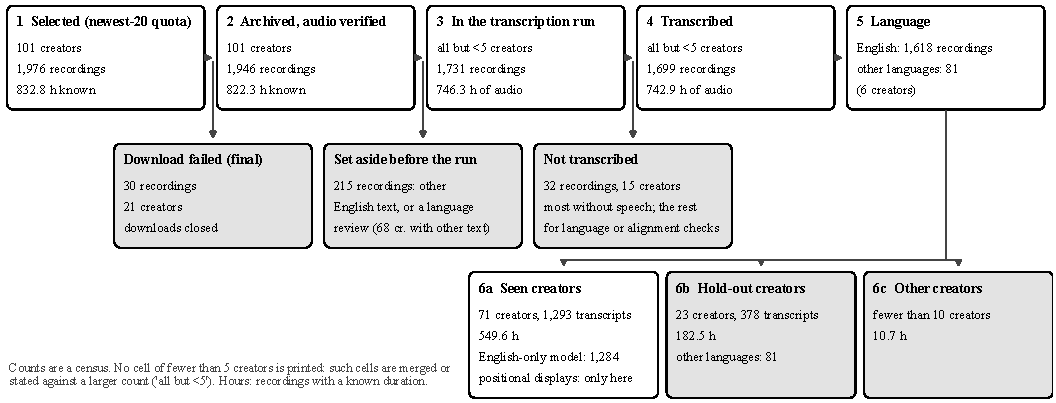
\includegraphics[width=\textwidth]{floats/fig_flow.pdf}
\caption{Coverage of the newest-20 quota, with every loss and its reason. Boxes give creators, recordings (transcripts in
the group boxes) and hours. Of \NSelected{} recordings of \NCreators{} creators, \NArchived{} were archived with
hash-verified audio and \NFailed{} are final download failures (\NFailedCreators{} creators). \NSetAside{} recordings
with English text of another kind (\NOtherTextCreators{} creators) or held for a language review were set aside, so
\NRunRecordings{} recordings (\RunHours{} h of audio) entered the run. \NTranscribedRecordings{} recordings
(\TranscribedHours{} h) were transcribed and \NNotTranscribed{} were not, most for want of speech. Census counts, in
recordings. No cell of fewer than 5 creators is printed: reasons are merged, and a creator count that falls fewer than 5
short of a printed total reads ``all but $<$5''.}
\label{fig:flow}
\end{figure*}

\paragraph{Three levels.} The \emph{creator} was selected as a medium; a \emph{recording} is of a kind (channelled
session, relayed message, interview, guided practice, own-voice talk, other); a \emph{span} is in a claimed, own or other
voice (Section~\ref{sec:protocol}). In an interim census of \LOneRecordings{} recordings of \LOneCreators{} development
creators, a claimed voice is the main kind of \LOneClaimedMainPct\% of recordings (creator-weighted; 95\%
\LOneClaimedMainLo--\LOneClaimedMainHi), and \LOneNoClaimedCreators{} creators (\LOneNoClaimedLo{} to \LOneNoClaimedHi{}
over model runs) have no sampled recording with a claimed voice in a quarter of its words; model-coded, not checked by a
person, interim (Table~\ref{tab:kinds}).

\paragraph{Dates.} Every selected recording has a date row: \NExactDays{} exact days and \NIntervalDates{} intervals
estimated from the displayed age. Local time stamps confirm \NConfirmedFromStamps{} intervals, so \NConfirmedDays{}
recordings have a confirmed day and \NStillInterval{} keep an interval (median width \IntervalMedianWidth{} days;
\NIntervalOverYear{} over a year). The published CSV prefixes the \NApostropheIds{} identifiers that begin with a hyphen
with an apostrophe. Dates are upload dates, not dates of speaking.

\paragraph{Agreement anchors and grid shift.} Table~\ref{tab:wer-strata} gives the strata of the caption anchor and of the
reproducibility row; Table~\ref{tab:gridshift} gives every measure of the grid shift. Moved here from Section 5.1 by
the page limit (fourth review round): halves at the median give \AnchorCaptionShortPct\% and \AnchorCaptionLongPct\% by
length and \AnchorCaptionLowConfPct\% and \AnchorCaptionHighConfPct\% by recognizer confidence (rough), strata added
after the reporting plan (addendum 1). In the bridge, numerals disagree \BridgeNumeralRatio{} times and capitalised
words \BridgeCapsRatio{} times as often as words overall (Section~\ref{sec:bridge}). The capped seam rule keeps
creators' rank order on every pause measure (rank correlation with no rule $\geq$ \SeamRuleRankCorrMin; moved here from
Section 5.3).

Moved here from Section 5 by the page limit (results round). \emph{Triangle inequality.} The run's edits against a true
transcript are at most its edits against the captions plus the captions' own edits, and at least their difference. As
rates, with $D$ the disagreement per caption word and $e$ the captions' own error rate, the run's error rate lies between
$|rD - e|$ and $rD + e$, where $r$, caption words over true words, is itself unknown within $1 \pm e$. Without $e$ the
bound says nothing: agreement (small $D$) shows only that the run's error is close to the captions' own error $e$, which
is unknown; and the bound concerns text after the normaliser, which lower-cases, drops fillers and expands
contractions. \emph{Grid shift by worker version.} The \GsEarlierVersionRecordings{} transcripts of record made by
earlier worker versions change less (mean \GsEarlierVersionMeanPct\%) than the other \GsSameVersionRecordings{} (mean
\GsSameVersionMeanPct\%, word-pooled \GsSameVersionPct\%), so the mixed headline does not inflate the grid effect. In
between-creator SD units every pause measure moves by at most \GsPauseSdMax{} on average and every word measure by at
most \GsWordSdMax, except filled pauses (\GsFillerSd; 95\% \GsFillerSdLo{} to \GsFillerSdHi); these are intervals, not
tests of equivalence. \emph{Precision check.} A phrase made by the grid should vanish when the grid moves, a spoken one
should recur. Of the \GsPrecisionRemoved{} removals in \GsPrecisionRecordings{} recordings, fewer than 5 creators have
a removal that recurs on the other grid; no share is printed from so small a count (Table~\ref{tab:gridshift-b}).

\begin{table}[ht]
\centering
\small
% tab_wer_strata.tex: GENERATED by WORK/build_numbers.py at 2026-11-22T00:15:32Z; label tab:wer-strata. The writer adds the float,
% the caption and the label. Sources: WER/out/wer-strata.csv
% Raw variant; halves added where thirds hold fewer than 5 creators (addendum 1). r: fewer than 12 creators; the percentile bootstrap covers below nominal there (rough).
{\scriptsize\setlength{\tabcolsep}{2pt}
\begin{tabular}{@{}p{0.3\linewidth}rrlll@{}}
\toprule
Stratum: level & Rec. & Cr. & Cr.\ mean [95\%] & Pooled [95\%] & Exact \% \\
\midrule
\multicolumn{6}{@{}p{0.97\linewidth}}{\emph{Captions (agreement)}} \\
audio edition: native & 11 & 11$^{r}$ & 3.8 [2.5, 5.2] & 4.9 [2.6, 7.2] & 0.0 \\
length third: high third & -- & $<$5 & \multicolumn{3}{l}{fewer than 5 creators} \\
length third: low third & -- & $<$5 & \multicolumn{3}{l}{fewer than 5 creators} \\
length third: middle third & -- & $<$5 & \multicolumn{3}{l}{fewer than 5 creators} \\
length half: lower half & 6 & 6$^{r}$ & 3.2 [1.9, 4.7] & 3.6 [2.2, 5.0] & 0.0 \\
length half: upper half & 5 & 5$^{r}$ & 4.4 [2.5, 6.9] & 5.2 [2.5, 7.6] & 0.0 \\
recognizer confidence third: high third & -- & $<$5 & \multicolumn{3}{l}{fewer than 5 creators} \\
recognizer confidence third: low third & -- & $<$5 & \multicolumn{3}{l}{fewer than 5 creators} \\
recognizer confidence third: middle third & -- & $<$5 & \multicolumn{3}{l}{fewer than 5 creators} \\
recognizer confidence half: lower half & 6 & 6$^{r}$ & 4.5 [2.2, 6.5] & 6.7 [2.8, 8.3] & 0.0 \\
recognizer confidence half: upper half & 5 & 5$^{r}$ & 2.9 [2.4, 3.5] & 2.7 [2.4, 3.5] & 0.0 \\
\multicolumn{6}{@{}p{0.97\linewidth}}{\emph{Same recognizer (reproducibility)}} \\
audio edition: native & -- & -- & \multicolumn{3}{l}{suppressed (gives a small cell by difference)} \\
audio edition: publisher & -- & $<$5 & \multicolumn{3}{l}{fewer than 5 creators} \\
length third: high third & 16 & 14 & \multicolumn{3}{l}{errors from fewer than 5 creators} \\
length third: low third & -- & -- & \multicolumn{3}{l}{suppressed (gives a small cell by difference)} \\
length third: middle third & 16 & 13 & \multicolumn{3}{l}{errors from fewer than 5 creators} \\
recognizer confidence third: high third & 16 & 15 & \multicolumn{3}{l}{errors from fewer than 5 creators} \\
recognizer confidence third: low third & 16 & 14 & \multicolumn{3}{l}{errors from fewer than 5 creators} \\
recognizer confidence third: middle third & 16 & 15 & \multicolumn{3}{l}{errors from fewer than 5 creators} \\
\bottomrule
\end{tabular}}

\caption{Agreement anchors by stratum, raw recognizer text: the platform-caption row by audio edition, by length half
and by recognizer-confidence half (thirds hold fewer than 5 creators), and the reproducibility row by length third.
Creator mean and word-pooled disagreement with 95\% creator percentile-bootstrap intervals; $r$ marks cells of fewer
than \MinCreatorsRegistered{} creators, below the smallest set size of this project's coverage audit, where such
intervals already cover below their nominal level (read as rough); a level or stratum whose values could be recovered by
difference, or whose errors come from fewer than 5 creators, is not printed. Halves and the confidence and edition strata were added after the
exploratory reporting plan (addendum 1, \AddendumOneStamp). Agreement of two machines, not an error rate.}
\label{tab:wer-strata}
\end{table}

\begin{table*}[tp]
\centering
\small
% tab_gridshift.tex: GENERATED by WORK/build_numbers.py at 2026-11-22T00:15:32Z; label tab:gridshift. The writer adds the float,
% the caption and the label. Sources: WER/out/gridshift-summary.csv; WER/out/gridshift-sd-units.csv; WER/out/gridshift-precision-check.csv
% Part 1 of 2. Shares in per cent; density ratios as ratios. Recordings = creators.
{\scriptsize\setlength{\tabcolsep}{2pt}
\begin{tabular}{@{}p{0.62\linewidth}lr@{}}
\toprule
Measure & Value [95\%] & Rec. \\
\midrule
changed share of words, shifted vs run grid (mean over recordings) & 3.7 [2.9, 4.9] & 40 \\
changed share of words, shifted vs run grid (word-pooled) & 4.2 [3.1, 5.4] & 40 \\
substitutions share, shifted vs run grid (word-pooled) & 1.7 [1.1, 2.4] & 40 \\
deletions share, shifted vs run grid (word-pooled) & 1.4 [1.0, 1.8] & 40 \\
insertions share, shifted vs run grid (word-pooled) & 1.1 [0.9, 1.3] & 40 \\
share of edits within 1 s of a run-grid seam (uniform expectation 0.0667) & 20.1 [17.5, 24.3] & 40 \\
share of edits within 1 s of a shifted-grid seam (uniform expectation 0.0667) & 18.6 [15.9, 23.0] & 40 \\
changed share of words, run grid decoded again vs transcript of record (word-pooled) & 0.0 [0.0, 0.0] & 10 \\
changed share, shifted minus control, same recordings (mean of differences) & 4.8 [2.4, 8.6] & 10 \\
changed share of words, shifted vs run grid, records made by the same worker version (word-pooled) & 4.3 [3.1, 5.6] & 31 \\
onset density in the first 0.25 s of windows / mean density: run-grid decode on its own grid & 1.92 [1.84, 2.01] & 40 \\
onset density in the last 0.25 s of windows / mean density: run-grid decode on its own grid & 0.60 [0.54, 0.66] & 40 \\
share of seams inside a pause of 0.3 s or more: run-grid decode on its own grid & 35.2 [30.0, 40.9] & 40 \\
share of seams inside a word: run-grid decode on its own grid & 0.0 [0.0, 0.0] & 40 \\
share of seams in a gap under 0.3 s: run-grid decode on its own grid & 64.8 [59.3, 70.1] & 40 \\
share of the time within 1 s of a seam inside pauses of 0.3 s or more: run-grid decode on its own grid & 20.8 [16.8, 25.6] & 40 \\
onset density in the first 0.25 s of windows / mean density: shifted decode on its own grid & 1.97 [1.88, 2.06] & 40 \\
onset density in the last 0.25 s of windows / mean density: shifted decode on its own grid & 0.59 [0.55, 0.64] & 40 \\
share of seams inside a pause of 0.3 s or more: shifted decode on its own grid & 35.6 [30.1, 41.9] & 40 \\
share of seams inside a word: shifted decode on its own grid & 0.0 [0.0, 0.0] & 40 \\
share of seams in a gap under 0.3 s: shifted decode on its own grid & 64.4 [58.1, 69.7] & 40 \\
share of the time within 1 s of a seam inside pauses of 0.3 s or more: shifted decode on its own grid & 22.1 [17.8, 27.2] & 40 \\
onset density in the first 0.25 s of windows / mean density: run-grid decode on the shifted grid (placebo) & 1.04 [1.00, 1.08] & 40 \\
onset density in the last 0.25 s of windows / mean density: run-grid decode on the shifted grid (placebo) & 0.94 [0.90, 0.99] & 40 \\
share of seams inside a pause of 0.3 s or more: run-grid decode on the shifted grid (placebo) & 22.3 [18.3, 26.9] & 40 \\
share of seams inside a word: run-grid decode on the shifted grid (placebo) & 72.1 [68.0, 75.8] & 40 \\
share of seams in a gap under 0.3 s: run-grid decode on the shifted grid (placebo) & 5.6 [4.3, 6.9] & 40 \\
share of the time within 1 s of a seam inside pauses of 0.3 s or more: run-grid decode on the shifted grid (placebo) & 22.4 [18.2, 26.9] & 40 \\
onset density in the first 0.25 s of windows / mean density: shifted decode on the run grid (placebo) & 1.01 [0.96, 1.06] & 40 \\
onset density in the last 0.25 s of windows / mean density: shifted decode on the run grid (placebo) & 0.96 [0.91, 1.00] & 40 \\
share of seams inside a pause of 0.3 s or more: shifted decode on the run grid (placebo) & 22.5 [18.3, 27.2] & 40 \\
share of seams inside a word: shifted decode on the run grid (placebo) & 71.2 [66.5, 75.4] & 40 \\
share of seams in a gap under 0.3 s: shifted decode on the run grid (placebo) & 6.3 [4.4, 8.7] & 40 \\
share of the time within 1 s of a seam inside pauses of 0.3 s or more: shifted decode on the run grid (placebo) & 21.4 [17.6, 25.7] & 40 \\
whole-recording pause share, run-grid decode & 20.3 [17.2, 23.9] & 40 \\
whole-recording pause share, shifted decode & 20.2 [16.8, 24.2] & 40 \\
whole-recording pause share, shifted minus run grid (mean of differences) & \ensuremath{-}0.14 [\ensuremath{-}0.58, 0.30] & 40 \\
words, shifted minus run grid, relative (mean of ratios minus 1) & \ensuremath{-}0.18 [\ensuremath{-}0.49, 0.04] & 40 \\
\bottomrule
\end{tabular}}

\caption{Grid shift, part 1: every measure with its 95\% interval from resampling the \GsRecordings{} recordings (one
per creator; raw recognizer words; grid moved by 15\,s). Controls: \GsControlIdentical{} recordings decoded again on
the run grid. Placebo rows measure a decode on the other grid.}
\label{tab:gridshift}
\end{table*}

\begin{table*}[tp]
\centering
\small
% tab_gridshift_b.tex: GENERATED by WORK/build_numbers.py at 2026-11-22T01:51:42Z; label tab:gridshift. The writer adds the float,
% the caption and the label. Sources: WER/out/gridshift-summary.csv; WER/out/gridshift-sd-units.csv; WER/out/gridshift-precision-check.csv
% Part 2 of 2. Shares in per cent; density ratios as ratios. Recordings = creators.
{\scriptsize\setlength{\tabcolsep}{2pt}
\begin{tabular}{@{}p{0.62\linewidth}lr@{}}
\toprule
Measure & Value [95\%] & Rec. \\
\midrule
\multicolumn{3}{@{}p{0.97\linewidth}}{\emph{Change, shifted minus run grid, in between-creator SD units (SD of seen creators' means on the transcripts of record): mean [95\%]. Percentiles over recordings are not printed: with 40 recordings each rests on 2 recordings (dominance rule)}} \\
Thanks-phrase segments per hour of speech (all, before the filter) (run grid 3.12, shifted grid 2.03 per speech hour) & \ensuremath{-}0.40 [\ensuremath{-}0.88, 0.08] & 40 \\
Thanks-phrase segments in the last 3 s of a window of the decode's own grid, per hour of speech (merged into the row of all segments of its family, because it would give a cell of fewer than 5 creators; plan section 3) & -- & -- \\
Thanks-phrase segments removed by the filter (all three thanks rules), per hour of speech (merged into the row of all segments of its family, because it would give a cell of fewer than 5 creators; plan section 3) & -- & -- \\
Isolated segments (5 s without speech on both sides) per hour of speech & 0.04 [\ensuremath{-}0.02, 0.15] & 40 \\
Isolated segments of 1 to 3 words removed by the filter, per hour of speech (merged into the row of all segments of its family, because it would give a cell of fewer than 5 creators; plan section 3) & -- & -- \\
Pauses of 0.3 to 1 s per minute of speech (BR) & \ensuremath{-}0.12 [\ensuremath{-}0.30, 0.03] & 40 \\
Pauses of 1 s or more per minute of speech (BR) & 0.01 [\ensuremath{-}0.05, 0.07] & 40 \\
Share of running time in pauses of 0.3 s or more (BR) & \ensuremath{-}0.02 [\ensuremath{-}0.07, 0.03] & 40 \\
Pauses of 0.3 s or more per 100 words (RH) & \ensuremath{-}0.08 [\ensuremath{-}0.19, 0.03] & 40 \\
Pauses of 1 s or more per 100 words (RH primary) & 0.01 [\ensuremath{-}0.05, 0.08] & 40 \\
Pauses of 2 s or more per 100 words (RH primary) & 0.03 [\ensuremath{-}0.05, 0.14] & 40 \\
Pauses of 2 s or more per minute of speech (RH delivery plane) & 0.02 [\ensuremath{-}0.05, 0.13] & 40 \\
Median pause of 0.3 s or more, seconds (RH) & 0.00 [\ensuremath{-}0.06, 0.05] & 40 \\
Share of running time in pauses of 2 s or more (RH) & 0.00 [\ensuremath{-}0.04, 0.04] & 40 \\
Pause share inside the speaking span (E4) & \ensuremath{-}0.02 [\ensuremath{-}0.07, 0.03] & 40 \\
Words per minute of the span without pauses of 0.3 s or more (E4) & \ensuremath{-}0.02 [\ensuremath{-}0.09, 0.05] & 40 \\
Words per minute of speech & 0.00 [\ensuremath{-}0.03, 0.01] & 40 \\
First-person singular per 1,000 words & 0.00 [\ensuremath{-}0.03, 0.03] & 40 \\
First-person plural per 1,000 words & 0.00 [\ensuremath{-}0.02, 0.02] & 40 \\
Second person per 1,000 words & 0.01 [\ensuremath{-}0.01, 0.03] & 40 \\
Contracted forms per 1,000 words & 0.04 [\ensuremath{-}0.01, 0.10] & 40 \\
Filled pauses per 1,000 words & 0.23 [\ensuremath{-}0.07, 0.69] & 40 \\
Share of distinct words in 100-word windows & 0.00 [\ensuremath{-}0.03, 0.02] & 40 \\
Mean word length (letters) & 0.02 [\ensuremath{-}0.01, 0.07] & 40 \\
Mean word length (seconds) & 0.02 [\ensuremath{-}0.06, 0.09] & 40 \\
\midrule
\multicolumn{3}{@{}p{0.97\linewidth}}{\emph{Positional rule checked on the re-decodes: a thanks phrase it removes should vanish when the grid moves; a spoken one should recur}} \\
run grid (transcript of record), searched in the shifted decode, tolerance 1 s: 55 removals in 22 recordings; fewer than 5 creators with a recurring removal & share not printed & 40 \\
run grid (transcript of record), searched in the shifted decode, tolerance 2 s: 55 removals in 22 recordings; fewer than 5 creators with a recurring removal & share not printed & 40 \\
shifted grid, searched in the run decode, tolerance 1 s: 37 removals in 19 recordings; fewer than 5 creators with a recurring removal & share not printed & 40 \\
shifted grid, searched in the run decode, tolerance 2 s: 37 removals in 19 recordings; fewer than 5 creators with a recurring removal & share not printed & 40 \\
\bottomrule
\end{tabular}}

\caption{Grid shift, part 2: the plan's thanks-phrase, isolated-segment and SD-unit rows, each change in units of the
SD of seen creators' means (all seen creators but fewer than 5 with three or more long transcripts), with its 95\%
interval from a seed per measure; percentiles over recordings are not printed, because with \GsRecordings{} recordings
each rests on a tail of fewer than 5 creators; rows that would give a cell of fewer than 5 creators by difference are
merged into the row of their family. Below, the positional rule checked on the re-decodes: removals and the count of
creators with a recurring removal, in the source's wording (fewer than 5, which includes none); no share or band of
shares is printed, since the source prints its band only when it includes 0, a rule that depends on the result.
Filter version 2 on each decode's own grid. No audio was played.}
\label{tab:gridshift-b}
\end{table*}

\paragraph{Artefact rules.} Table~\ref{tab:artefacts} gives every rule of filter version 2 (Section~\ref{sec:artefacts}).
Moved here from Section 5.4 by the page limit (fourth review round): the window-end thanks phrase appears in
\ThanksPerWindowPct\% of windows mostly covered by other speech (90\% \ThanksPerWindowLo--\ThanksPerWindowHi) and in
\ThanksPerWindowPartialPct\% of partly covered windows; all but fewer than 5 of the \NSeen{} seen creators have one;
\ThanksTranscriptPct\% of transcripts hold one at a window end, a share that ranges from \ThanksWeightRangeLo{} to
\ThanksWeightRangeHi{} over weightings and is not a headline.

% Moved here from Section 5.4 by the page limit (third review round); caption unchanged.
\begin{table}[ht]
\centering
\small
% tab_artefacts.tex: GENERATED by WORK/build_numbers.py at 2026-11-22T01:51:42Z; label tab:artefacts. The writer adds the float,
% the caption and the label. Sources: REV/build-robustness/out/R7/R7-artefact-rules.csv
% Base: English-only seen transcripts; creators out of the seen creators.
{\scriptsize\setlength{\tabcolsep}{2pt}
\begin{tabular}{@{}p{0.21\linewidth}rrp{0.12\linewidth}p{0.07\linewidth}p{0.12\linewidth}p{0.15\linewidth}@{}}
\toprule
Rule (filter v2) & Rem. & Per 1{,}000 win. & Transcr.\ \% [90\%] & Cr. & Per speech h [90\%] & Bound, phase counts \\
\midrule
Thanks phrase in a window's last 3 s & 1{,}422 & 21.8 & 49.9\newline[45.2, 54.5] & all but $<$5 & 2.95\newline[2.73, 3.19] & 0.949-0.977 (point 0.97) \\
Thanks phrase, low probability & 30 & 0.46 & 2.1\newline[1.3, 3.1] & 19 & 0.06\newline[0.04, 0.09] & $\geq$ 0.80 \\
Thanks phrase, isolated & 71 & 1.1 & 2.9\newline[1.8, 4.1] & 19 & 0.15\newline[0.08, 0.23] & not bounded (shares the isolated rule) \\
Isolated segment, $\leq$3 words & 191 & 2.9 & 6.9\newline[4.6, 9.5] & 30 & 0.40\newline[0.24, 0.59] & $\geq$ 0.63 \\
Stock or credit text & 8 & 0.12 & 0.6\newline[0.2, 1.1] & 6 & 0.02\newline[0.01, 0.03] & $\geq$ 0.55 \\
Fourth and later repeat & 13 & 0.20 & 0.7\newline[0.2, 1.2] & 7 & 0.03\newline[0.01, 0.05] & $\geq$ 0.29 \\
Words removed as loops (words) & 4{,}219 & 64.8 & 23.0\newline[18.6, 27.4] & 56 & 8.76\newline[4.62, 13.74] & $\geq$ 0.14 (weak) \\
\bottomrule
\end{tabular}}

\caption{Recognizer artefacts by rule of filter version 2, \NSeenEnglishOnly{} English-only transcripts of \NSeen{} seen
creators (full 30-s windows): units removed, removed with the isolated rule off, per 1,000 full windows, share of
transcripts with one (90\% creator bootstrap), creators with one, rate per speech hour (90\%), and the precision bound
from window-phase counts (which assumes spoken phrases spread evenly over window phase). Nothing was checked by a person.}
\label{tab:artefacts}
\end{table}

\paragraph{Headline numbers and their drift.} Table~\ref{tab:headlines} (Table U) states each headline number with its
estimand, weighting, interval and counts; Table~\ref{tab:drift} (Table D) sets each against the earlier draft's snapshot.

% INTEGRATOR (2026-11-21): Table U is taller than a page; the builder writes it in two parts of consecutive rows.
\begin{table*}[tp]
\centering
\small
% tab_headlines.tex: GENERATED by the private builder build_numbers.py at 2026-11-26T03:59:48Z; label tab:headlines. The writer adds the float,
% the caption and the label. Sources: a private file of the run (named in the private build record)
% Part 1 of 2. Table U (D4); rows that are a minimum or maximum over measures, or not regenerable, or a percentile in a tail of fewer than 5 creators, are left out. ICC rows here are one-way ANOVA ICC(1) on raw recording values; the variance partition (tab:vp) gives each measure on its named scale.
{\scriptsize\setlength{\tabcolsep}{2pt}
\begin{tabular}{@{}p{0.27\textwidth}p{0.25\textwidth}p{0.12\textwidth}lp{0.06\textwidth}rr@{}}
\toprule
Quantity & Estimand & Weighting & Value [95\%] & Unit & Cr. & Rec. \\
\midrule
selected recordings & census count & none & 1{,}976 &  & -- & -- \\
archived with verified audio & census count & none & 1{,}946 &  & -- & -- \\
final download failures & census count & none & 30 &  & -- & -- \\
share of run audio files transcribed & census share & recording-equal & 98.1 & \% & -- & -- \\
audio hours transcribed & census sum & hour-pooled & 742.9 & h & -- & -- \\
audio files not in English & census count & none & 81 &  & 6 & -- \\
share of audio without speech (voice detector) & share of audio seconds outside the detector's speech & hour-pooled & 12.1 [7.7, 17.5] & \% & 71 & 1{,}293 \\
share of audio without speech (voice detector) & mean over creators of the creator's pooled share & creator-equal & 12.2 [8.7, 15.6] & \% & 71 & 1{,}293 \\
share of audio without speech (voice detector) & median over creators of the creator's pooled share & creator median & 7.9 [5.3, 10.8] & \% & 71 & 1{,}293 \\
share of non-speech time held by the five creators with most & concentration share & hour-pooled & 46.0 [21.7, 57.8] & \% & 71 & 1{,}293 \\
recordings at least half without speech & count & recording-equal & 62 &  & 21 & 1{,}293 \\
recordings under 50 words & count & recording-equal & 19 &  & 10 & 1{,}293 \\
hours in stretches of 30 s or more outside segments & sum & hour-pooled & 28.6 [8.3, 60.7] & h & 71 & 1{,}293 \\
recordings with a stretch of 30 s or more & count & recording-equal & 216 &  & 42 & 1{,}293 \\
median recording length & median over audio files & recording-equal & 17.8 [15.1, 21.4] & min & all but $<$5 & all \\
median recording length, creator-equal & median of creator medians & creator median & 19.6 & min & all but $<$5 & all \\
median recording length, creator-equal, seen creators & median of creator medians & creator median & 19.3 & min & 71 & 1{,}293 \\
first quartile of length & quantile over audio files & recording-equal & 8.3 & min & -- & -- \\
third quartile of length & quantile over audio files & recording-equal & 36.3 & min & -- & -- \\
recordings of 5 min or less & count & recording-equal & 269 &  & -- & -- \\
recordings over 60 min & count & recording-equal & 167 &  & -- & -- \\
median words per transcript & median over transcripts & recording-equal & 2{,}120 [1675, 2700] & words & 71 & 1{,}293 \\
median pace & median over English recordings with 1 min or more of speech & recording-equal & 148.2 [144.3, 153.3] & words per speech minute & 71 & 1{,}231 \\
median pace, creator-equal & median of creator medians & creator median & 148.7 & words per speech minute & 71 & 1{,}231 \\
first quartile of pace & quantile & recording-equal & 133.7 & wpm & -- & -- \\
third quartile of pace & quantile & recording-equal & 163.0 & wpm & -- & -- \\
\bottomrule
\end{tabular}}

\caption{Table U, part 1: each headline number of this paper with its estimand, weighting, 95\% interval ($t$ on
creator means for means of creator values; creator bootstrap otherwise), creators and recordings, on the closed run.
Counts, durations and languages cover all creators; every number from text, segments or the voice detector covers the
\NSeen{} seen creators. Counts follow D4's definitions and can differ from the filter's counts of
Table~\ref{tab:artefacts} (for example, the share of transcripts with a bare thanks segment anywhere); D4's counts of
isolated short segments are not printed, because beside each other and beside the filter's counts they differ by cells
of fewer than 5 creators (Table~\ref{tab:artefacts} gives the filter's); census counts are in recordings
(Section~\ref{sec:data}), and ``all'' in the last column means every transcript of the run; ICC rows are one-way ANOVA ICC(1) on raw recording values, while Table~\ref{tab:vp}
gives each measure on its named scale. A percentile in a tail of fewer than 5 creators is not printed.}
\label{tab:headlines}
\end{table*}

\begin{table*}[tp]
\centering
\small
% tab_headlines_b.tex: GENERATED by WORK/build_numbers.py at 2026-11-22T01:51:42Z; label tab:headlines. The writer adds the float,
% the caption and the label. Sources: REV/build-descriptive/out/D4/D4-table-U.csv
% Part 2 of 2. Table U (D4); rows that are a minimum or maximum over measures, or not regenerable, or a percentile in a tail of fewer than 5 creators, are left out. ICC rows here are one-way ANOVA ICC(1) on raw recording values; the variance partition (tab:vp) gives each measure on its named scale.
{\scriptsize\setlength{\tabcolsep}{2pt}
\begin{tabular}{@{}p{0.27\textwidth}p{0.25\textwidth}p{0.12\textwidth}lp{0.06\textwidth}rr@{}}
\toprule
Quantity & Estimand & Weighting & Value [95\%] & Unit & Cr. & Rec. \\
\midrule
ICC(1) lexical variety (MATTR-500) [one-way ANOVA ICC(1) on the raw recording values] & share of recording-level variance between creators (one-way ANOVA ICC(1)) & recording-level, creators as groups & 0.6 [0.48, 0.7] &  & all but $<$5 & 1{,}113 \\
ICC(1) pace (words per speech minute) [one-way ANOVA ICC(1) on the raw recording values] & share of recording-level variance between creators (one-way ANOVA ICC(1)) & recording-level, creators as groups & 0.58 [0.46, 0.66] &  & 71 & 1{,}231 \\
ICC(1) share without speech (detector) [one-way ANOVA ICC(1) on the raw recording values] & share of recording-level variance between creators (one-way ANOVA ICC(1)) & recording-level, creators as groups & 0.51 [0.26, 0.7] &  & 71 & 1{,}231 \\
ICC(1) mean segment log-probability [one-way ANOVA ICC(1) on the raw recording values] & share of recording-level variance between creators (one-way ANOVA ICC(1)) & recording-level, creators as groups & 0.41 [0.15, 0.64] &  & 71 & 1{,}231 \\
ICC(1) length (log minutes) [one-way ANOVA ICC(1) on the raw recording values] & share of recording-level variance between creators (one-way ANOVA ICC(1)) & recording-level, creators as groups & 0.42 [0.31, 0.52] &  & 71 & 1{,}231 \\
ICC(1) share of segments ending in ? [one-way ANOVA ICC(1) on the raw recording values] & share of recording-level variance between creators (one-way ANOVA ICC(1)) & recording-level, creators as groups & 0.27 [0.21, 0.34] &  & 71 & 1{,}231 \\
ICC(1) repeated five-word share [one-way ANOVA ICC(1) on the raw recording values] & share of recording-level variance between creators (one-way ANOVA ICC(1)) & recording-level, creators as groups & 0.25 [0.13, 0.45] &  & all but $<$5 & 1{,}220 \\
share of the first tenth covered by segments & creator-equal mean of recording coverage & creator-equal & 0.83 [0.8, 0.86] &  & 71 & 1{,}293 \\
share of the last tenth covered by segments & creator-equal mean of recording coverage & creator-equal & 0.73 [0.69, 0.78] &  & 71 & 1{,}293 \\
Spearman: log-probability and pace (recording level, pooled) & pooled rank correlation & recording-equal & 0.49 [0.38, 0.58] &  & 71 & 1{,}231 \\
Spearman: log-probability and pace, between creators & rank correlation of creator medians & creator-equal & 0.54 [0.35, 0.69] &  & 71 & 1{,}231 \\
Spearman: log-probability and pace, within creators & rank correlation of creator-centred values & recording-equal within creator & 0.43 [0.36, 0.5] &  & 71 & 1{,}231 \\
Spearman: log-probability and share without speech (pooled) & pooled rank correlation & recording-equal & \ensuremath{-}0.43 [\ensuremath{-}0.55, \ensuremath{-}0.31] &  & 71 & 1{,}231 \\
Spearman: log-probability and length (pooled) & pooled rank correlation & recording-equal & \ensuremath{-}0.0 [\ensuremath{-}0.11, 0.1] &  & 71 & 1{,}231 \\
transcripts with a bare two-word thanks segment [D4's definition] & share of transcripts & recording-equal & 55.5 [50.4, 60.3] & \% & 71 & 1{,}293 \\
transcripts with a bare thanks segment, creator-equal [D4's definition] & mean of creator shares & creator-equal & 55.2 [49.8, 60.5] & \% & 71 & 1{,}293 \\
bare thanks segments & count & segment & 1{,}770 &  & -- & -- \\
thanks segments starting 27-30 s into a window & share of segments & segment-pooled & 81 [77, 84] & \% & 71 & 718 \\
thanks segments with under 1 s gap on both sides & share of segments & segment-pooled & 84 [81, 87] & \% & -- & -- \\
median log-probability of thanks segments & median over segments & segment-pooled & \ensuremath{-}0.71 &  & -- & -- \\
median log-probability of other segments of 3 words or fewer & median over segments & segment-pooled & \ensuremath{-}0.22 &  & -- & -- \\
isolated segments starting on a multiple of 30 s (thanks included, as the reading notes) & share of segments & segment-pooled & 39 & \% & -- & -- \\
isolated segments starting on a multiple of 30 s (thanks excluded) & share of segments & segment-pooled & 36 & \% & -- & -- \\
window span of a creator's newest 20 & median over creators & creator-equal & 164 & days & 101 & -- \\
creators whose newest 20 fit in 30 days & count & creator & 8 &  & 101 & -- \\
creators needing more than two years & count & creator & 10 &  & 101 & -- \\
\bottomrule
\end{tabular}}

\caption{Table U, part 2 (columns as in part 1).}
\label{tab:headlines-b}
\end{table*}

% INTEGRATOR (2026-11-21): Table D is taller than a page; the builder writes it in two parts of consecutive rows.
\begin{table*}[tp]
\centering
\small
% tab_drift.tex: GENERATED by the private builder build_numbers.py at 2026-11-26T03:59:48Z; label tab:drift. The writer adds the float,
% the caption and the label. Sources: a private file of the run (named in the private build record)
% Part 1 of 2. Table D (D4): the old draft's snapshot numbers against the closed run.
{\scriptsize\setlength{\tabcolsep}{2pt}
\begin{tabular}{@{}p{0.34\linewidth}p{0.3\linewidth}lll@{}}
\toprule
Quantity & Comparison & Snapshot & Closed run & Diff. \\
\midrule
selected recordings & same estimand and base & 1{,}976 & 1{,}976 & 0 \\
archived with verified audio & same estimand and base & 1{,}946 & 1{,}946 & 0 \\
final download failures & same estimand and base & 30 & 30 & 0 \\
share of run audio files transcribed & same estimand and base & 95 & 98.1 & 3.1 \\
audio hours transcribed & same estimand and base & 510.8 & 742.9 & 232.1 \\
audio files not in English & same estimand and base & 12 & 81 & 69 \\
share of audio without speech (voice detector) & same estimand; creator set differs (snapshot: all creators; not shown) & -- & 12.1 & -- \\
share of audio without speech (voice detector) & new estimand: the snapshot has no value of this estimand & -- & 12.2 & -- \\
share of audio without speech (voice detector) & same estimand and creators (71 seen creators; the snapshot had fewer transcripts) & 7.9 & 7.9 & 0 \\
share of non-speech time held by the five creators with most & same estimand; creator set differs (snapshot: all creators; not shown) & -- & 46 & -- \\
recordings at least half without speech & same estimand; creator set differs (snapshot: all creators; not shown) & -- & 62 & -- \\
recordings under 50 words & same estimand; creator set differs (snapshot: all creators; not shown) & -- & 19 & -- \\
hours in stretches of 30 s or more outside segments & same estimand; creator set differs (snapshot: all creators; not shown) & -- & 28.6 & -- \\
recordings with a stretch of 30 s or more & same estimand; creator set differs (snapshot: all creators; not shown) & -- & 216 & -- \\
median recording length & same estimand and base & 17.3 & 17.8 & 0.5 \\
median recording length, creator-equal & no snapshot value on this base: the snapshot's creator medians cover the 71 seen creators only (see the next row) & -- & 19.6 & -- \\
median recording length, creator-equal, seen creators & same estimand and creators (71 seen creators; the snapshot had fewer transcripts) & 18.5 & 19.3 & 0.8 \\
first quartile of length & same estimand and base & 8.3 & 8.3 & 0 \\
third quartile of length & same estimand and base & 35.7 & 36.3 & 0.6 \\
recordings of 5 min or less & same estimand and base & 192 & 269 & 77 \\
recordings over 60 min & same estimand and base & 106 & 167 & 61 \\
median words per transcript & same estimand; creator set differs (snapshot: all creators; not shown) & -- & 2{,}120 & -- \\
median pace & same estimand and creators (71 seen creators; the snapshot had fewer transcripts) & 148 & 148.2 & 0.2 \\
median pace, creator-equal & same estimand and creators (71 seen creators; the snapshot had fewer transcripts) & 147 & 148.7 & 1.7 \\
first quartile of pace & same estimand and creators (71 seen creators; the snapshot had fewer transcripts) & 134 & 133.7 & -0.3 \\
third quartile of pace & same estimand and creators (71 seen creators; the snapshot had fewer transcripts) & 163 & 163 & 0 \\
ICC(1) lexical variety (MATTR-500) & same estimand and creators (71 seen creators; the snapshot had fewer transcripts) & 0.61 & 0.6 & -0.01 \\
ICC(1) pace (words per speech minute) & same estimand and creators (71 seen creators; the snapshot had fewer transcripts) & 0.57 & 0.58 & 0.01 \\
\bottomrule
\end{tabular}}

\caption{Table D, part 1: drift from the earlier draft's snapshot (\SnapLines{} transcripts) to the closed run, like
with like. Where the snapshot had no such estimand, or another definition, its cells read ``--''; so do snapshot values
computed from the transcripts or timing of all creators, hold-out included, which are not printed. A difference also
mixes more transcripts. ICCs here are point values; their intervals for the closed run are in Table~\ref{tab:headlines}
and Table~\ref{tab:vp}.}
\label{tab:drift}
\end{table*}

\begin{table*}[tp]
\centering
\small
% tab_drift_b.tex: GENERATED by WORK/build_numbers.py at 2026-11-22T00:15:32Z; label tab:drift. The writer adds the float,
% the caption and the label. Sources: REV/build-descriptive/out/D4/D4-table-D-drift.csv
% Part 2 of 2. Table D (D4): the old draft's snapshot numbers against the closed run.
{\scriptsize\setlength{\tabcolsep}{2pt}
\begin{tabular}{@{}p{0.34\linewidth}p{0.3\linewidth}lll@{}}
\toprule
Quantity & Comparison & Snapshot & Closed run & Diff. \\
\midrule
ICC(1) share without speech (detector) & same estimand and creators (71 seen creators; the snapshot had fewer transcripts) & 0.5 & 0.51 & 0.01 \\
ICC(1) mean segment log-probability & same estimand and creators (71 seen creators; the snapshot had fewer transcripts) & 0.41 & 0.41 & 0 \\
ICC(1) length (log minutes) & same estimand and creators (71 seen creators; the snapshot had fewer transcripts) & 0.43 & 0.42 & -0.01 \\
ICC(1) share of segments ending in ? & same estimand and creators (71 seen creators; the snapshot had fewer transcripts) & 0.29 & 0.27 & -0.02 \\
ICC(1) repeated five-word share & same estimand and creators (71 seen creators; the snapshot had fewer transcripts) & 0.24 & 0.25 & 0.01 \\
smallest ICC of the seven & same estimand; creator set differs (snapshot: all creators; not shown) & -- & 25 & -- \\
largest ICC of the seven & same estimand; creator set differs (snapshot: all creators; not shown) & -- & 60 & -- \\
share of the first tenth covered by segments & same estimand and creators (71 seen creators; the snapshot had fewer transcripts) & 0.83 & 0.83 & 0 \\
share of the last tenth covered by segments & same estimand and creators (71 seen creators; the snapshot had fewer transcripts) & 0.73 & 0.73 & 0 \\
largest tenth coverage & same estimand and creators (71 seen creators; the snapshot had fewer transcripts) & 0.88 & 0.88 & 0 \\
Spearman: log-probability and pace (recording level, pooled) & same estimand; creator set differs (snapshot: all creators; not shown) & -- & 0.49 & -- \\
Spearman: log-probability and pace, between creators & same estimand and creators (71 seen creators; the snapshot had fewer transcripts) & 0.5 & 0.54 & 0.04 \\
Spearman: log-probability and pace, within creators & new estimand: the snapshot has no value of this estimand & -- & 0.43 & -- \\
Spearman: log-probability and share without speech (pooled) & same estimand; creator set differs (snapshot: all creators; not shown) & -- & -0.43 & -- \\
Spearman: log-probability and length (pooled) & same estimand; creator set differs (snapshot: all creators; not shown) & -- & -0 & -- \\
transcripts with a bare two-word thanks segment & same estimand as one reader's notes (snapshot: all creators; not shown) & -- & 55.5 & -- \\
transcripts with a bare thanks segment, creator-equal & new estimand: the snapshot has no value of this estimand & -- & 55.2 & -- \\
bare thanks segments & same estimand as one reader's notes (snapshot: all creators; not shown) & -- & 1{,}770 & -- \\
thanks segments starting 27-30 s into a window & same estimand as one reader's notes (snapshot: all creators; not shown) & -- & 81 & -- \\
thanks segments with under 1 s gap on both sides & same estimand as one reader's notes (snapshot: all creators; not shown) & -- & 84 & -- \\
median log-probability of thanks segments & same estimand as one reader's notes (snapshot: all creators; not shown) & -- & -0.71 & -- \\
median log-probability of other segments of 3 words or fewer & same estimand as one reader's notes (snapshot: all creators; not shown) & -- & -0.22 & -- \\
isolated segments starting on a multiple of 30 s (thanks included, as the reading notes) & same estimand as one reader's notes (snapshot: all creators; not shown) & -- & 39 & -- \\
isolated segments starting on a multiple of 30 s (thanks excluded) & different definition from the reading notes (thanks segments excluded): not compared & -- & 36 & -- \\
window span of a creator's newest 20 & same estimand and base & 164 & 164 & 0 \\
creators whose newest 20 fit in 30 days & same estimand and base & 8 & 8 & 0 \\
creators needing more than two years & same estimand and base & 10 & 10 & 0 \\
\bottomrule
\end{tabular}}

\caption{Table D, part 2 (columns as in part 1).}
\label{tab:drift-b}
\end{table*}

\paragraph{Coverage by rank and balance of the groups.} Figure~\ref{fig:rank} and Table~\ref{tab:rank-odds} show how the
run's coverage depends on listing rank (Section~\ref{sec:coverage}). Figure~\ref{fig:love} and Table~\ref{tab:balance}
show how the hold-out differs from the seen creators on fields known before the run (Section~\ref{sec:holdout}); a
difference between them is never a replication or a failed replication.

\begin{figure}[ht]
\centering
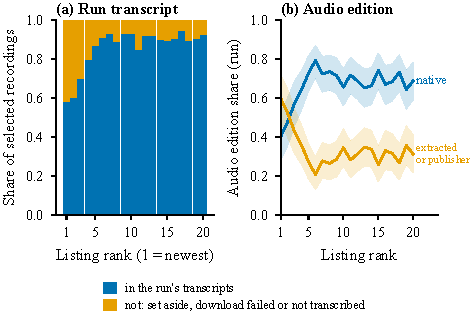
\includegraphics[width=\columnwidth]{floats/fig_rank.pdf}
\caption{Coverage of the newest-20 quota by listing rank (1 is the newest; listing order, not time): (a) share of the
\NSelected{} selected recordings with a run transcript and without one (set aside, download failed or not transcribed,
merged); (b) share of native platform audio among the recordings in the run, and of the other editions merged, with
95\% creator-bootstrap bands. A creator has at most one recording at a rank, so each cell is a count of creators, and
every cell holds 5 or more; the split by reason is in Table~\ref{tab:rank-odds}. Description of coverage; no trend is
read from rank.}
\label{fig:rank}
\end{figure}

\begin{table*}[tp]
\centering
\small
% tab_rank_odds.tex: GENERATED by the private builder build_numbers.py at 2026-11-26T03:59:48Z; label tab:rank-odds. The writer adds the float,
% the caption and the label. Sources: a private file of the run (named in the private build record)
% Creator-stratified Mantel-Haenszel and pooled ORs with 95% creator bootstrap; SMDs with 90% creator bootstrap. n.p.: the creators of 'no text of any kind' are not printed (D49).
{\scriptsize\setlength{\tabcolsep}{2pt}
\begin{tabular}{@{}p{0.36\textwidth}llll@{}}
\toprule
Outcome (ranks 1--5 against 6--20) & Pooled OR [95\%] & MH OR [95\%] & Cond.\ logit [95\% Wald] & Cr. \\
\midrule
not transcribed (any reason) & 4.12 [2.70, 6.95] & 5.47 [3.34, 9.75] & 7.15 [5.11, 10.0] & 84 \\
no text of any kind (download failed or not transcribed) & 1.04 [0.52, 1.92] & 1.04 [0.50, 1.95] & 1.04 [0.57, 1.89] & n.p. \\
other text kind or language review & 5.57 [3.28, 13.4] & 10.4 [4.97, 33.9] & 19.5 [11.8, 32.4] & 68 \\
\midrule
\multicolumn{5}{@{}p{0.97\linewidth}}{\emph{Transcribed (T) against other text (O) and missing (M): SMD [90\%]}} \\
log length (minutes; metadata, inventory or catalogue) & O: 0.12 [\ensuremath{-}0.03, 0.26] & M: \ensuremath{-}0.76 [\ensuremath{-}1.07, \ensuremath{-}0.44] &  &  \\
listing rank (1 = newest) & O: \ensuremath{-}0.76 [\ensuremath{-}1.14, \ensuremath{-}0.53] & M: \ensuremath{-}0.09 [\ensuremath{-}0.34, 0.13] &  &  \\
rank 1 to 5 (share) & O: 0.87 [0.62, 1.31] & M: 0.11 [\ensuremath{-}0.11, 0.36] &  &  \\
date evidence E1, confirmed day (share) & O: \ensuremath{-}0.61 [\ensuremath{-}0.95, \ensuremath{-}0.25] & M: 0.12 [\ensuremath{-}0.15, 0.39] &  &  \\
date evidence E3, still estimated (share) & O: 0.86 [0.49, 1.21] & M: \ensuremath{-}0.35 [\ensuremath{-}0.51, \ensuremath{-}0.14] &  &  \\
audio from the platform video (share of recordings with audio) & O: -- & M: 0.36 [0.24, 0.46] &  &  \\
publisher audio edition (share of recordings with audio) & O: -- & M: \ensuremath{-}0.36 [\ensuremath{-}0.46, \ensuremath{-}0.24] &  &  \\
log(1 + views at capture), seen creators only & O: 0.15 [\ensuremath{-}0.10, 0.42] & M: \ensuremath{-}0.14 [\ensuremath{-}0.45, 0.18] &  &  \\
\bottomrule
\end{tabular}}

\caption{Missingness by listing rank and recording properties. Top: odds ratios for ranks 1--5 against 6--20, pooled
(0.5 added per cell), Mantel--Haenszel within creator and conditional logit, with 95\% creator-bootstrap intervals, and
the creators with variation in the outcome. Bottom: standardized mean differences of recordings with other text (O) and
of recordings with no text (M) against transcribed recordings, with 90\% creator-bootstrap intervals. Event counts and
group sizes are not printed: beside the census counts some would give a cell of fewer than 5 by difference.}
\label{tab:rank-odds}
\end{table*}

\begin{figure}[ht]
\centering
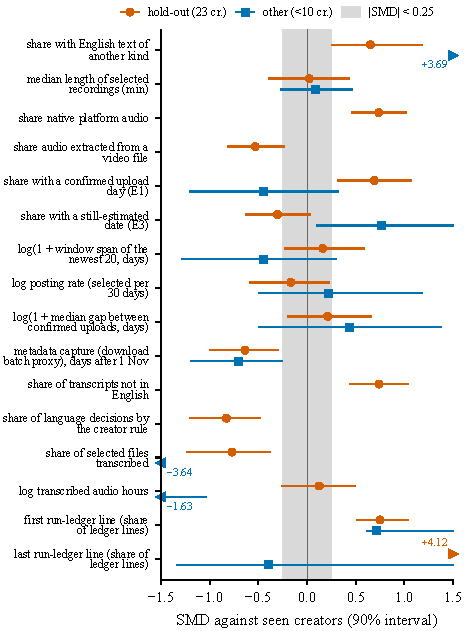
\includegraphics[width=\columnwidth]{floats/fig_love.pdf}
\caption{Standardized mean differences of creator values on ledger and inventory fields only: hold-out (\NHoldout)
minus seen (\NSeen) and other (\NOtherCreators) minus seen, with 90\% intervals from creator resamples within group,
clipped at $\pm$1 (values beyond the edge printed beside it); dashed lines $\pm$0.25, dotted $\pm$0.1. With
\NOtherCreators{} creators the other group's differences are unstable. The binary roster-vintage field is not drawn
(its signed differences would give group cells of fewer than 5 creators), and neither is a group's difference that
rests on fewer than 5 creators with a value other than the group's common one, nor a field where the seen group has
1 to 4 such creators. No transcript field of a non-seen creator was read.}
\label{fig:love}
\end{figure}

\begin{table*}[tp]
\centering
\small
% tab_balance.tex: GENERATED by the private builder build_numbers.py at 2026-11-26T03:59:48Z; label tab:balance. The writer adds the float,
% the caption and the label. Sources: a private file of the run (named in the private build record)
% Counts, durations, dates, languages and run order only (not contacts).
{\scriptsize\setlength{\tabcolsep}{2pt}
\begin{tabular}{@{}p{0.30\textwidth}clllll@{}}
\toprule
Covariate & Block & Seen: median (IQR) & Hold-out: median (IQR) & SMD hold-out [90\%] & SMD other [90\%] \\
\midrule
share with English text of another kind & A & 0.05 (0.00--0.10) & 0.10 (0.05--0.15) & 0.65 [0.26, 1.18] & 3.69 [3.16, 5.70] \\
median length of selected recordings (min) & A & 18.68 (11.01--28.79) & 15.85 (9.64--33.38) & 0.02 [\ensuremath{-}0.39, 0.43] & 0.08 [\ensuremath{-}0.27, 0.46] \\
share native platform audio & A & 0.76 (0.42--0.89) & 0.84 (0.78--0.90) & 0.74 [0.46, 1.02] & -- \\
share audio extracted from a video file & A & 0.20 (0.09--0.46) & 0.16 (0.10--0.20) & \ensuremath{-}0.53 [\ensuremath{-}0.81, \ensuremath{-}0.24] & -- \\
share with a confirmed upload day (E1) & A & 0.90 (0.70--0.95) & 0.95 (0.90--1.00) & 0.69 [0.32, 1.07] & \ensuremath{-}0.45 [\ensuremath{-}1.20, 0.31] \\
share with a still-estimated date (E3) & A & 0.05 (0.00--0.10) & 0.05 (0.00--0.10) & \ensuremath{-}0.30 [\ensuremath{-}0.62, 0.03] & 0.77 [0.10, 1.59] \\
log(1 + window span of the newest 20, days) & A & 5.04 (4.52--6.27) & 5.67 (4.91--5.97) & 0.16 [\ensuremath{-}0.23, 0.58] & \ensuremath{-}0.45 [\ensuremath{-}1.28, 0.29] \\
log posting rate (selected per 30 days) & A & 1.36 (0.13--1.89) & 0.73 (0.43--1.49) & \ensuremath{-}0.17 [\ensuremath{-}0.58, 0.22] & 0.22 [\ensuremath{-}0.49, 1.18] \\
log(1 + median gap between confirmed uploads, days) & A & 2.08 (1.50--2.30) & 2.08 (1.79--2.74) & 0.21 [\ensuremath{-}0.20, 0.66] & 0.43 [\ensuremath{-}0.49, 1.37] \\
metadata capture (download batch proxy), days after 1 Nov & A & 17.75 (17.34--18.93) & 17.75 (17.34--17.77) & \ensuremath{-}0.64 [\ensuremath{-}0.99, \ensuremath{-}0.30] & \ensuremath{-}0.71 [\ensuremath{-}1.19, \ensuremath{-}0.26] \\
share of transcripts not in English & L & 0.00 (0.00--0.00) & 0.00 (--) & 0.74 [0.44, 1.03] & -- \\
share of language decisions by the creator rule & L & 0.84 (0.80--0.88) & 0.83 (0.27--0.88) & \ensuremath{-}0.83 [\ensuremath{-}1.20, \ensuremath{-}0.48] & -- \\
share of selected files transcribed & R & 0.90 (0.90--0.95) & 0.85 (0.80--0.91) & \ensuremath{-}0.77 [\ensuremath{-}1.23, \ensuremath{-}0.38] & \ensuremath{-}3.64 [\ensuremath{-}5.64, \ensuremath{-}3.07] \\
log transcribed audio hours & R & 1.94 (1.41--2.38) & 1.99 (1.51--2.36) & 0.13 [\ensuremath{-}0.26, 0.49] & \ensuremath{-}1.63 [\ensuremath{-}2.92, \ensuremath{-}1.04] \\
first run-ledger line (share of the run's ledger lines) & Q & 0.03 (0.01--0.04) & 0.08 (0.03--0.12) & 0.75 [0.51, 1.04] & 0.71 [0.62, 1.61] \\
last run-ledger line (share of the run's ledger lines) & Q & 0.76 (0.75--0.77) & 0.95 (0.95--0.96) & 4.12 [2.92, 10.48] & \ensuremath{-}0.40 [\ensuremath{-}1.33, 2.55] \\
\midrule
\multicolumn{6}{@{}p{0.97\linewidth}}{\emph{Roster vintage, all creators: 74 original, 27 added on the day of the listing}} \\
\multicolumn{6}{@{}p{0.97\linewidth}}{\emph{Hold-out membership AUC: A 0.69 (shuffle 95\% band 0.30--0.67); A + language decisions 0.84 (shuffle 95\% band 0.32--0.66)}} \\
\bottomrule
\end{tabular}}

\caption{Table B: balance of the seen, hold-out and other creators on fields known before the run, with medians and
quartiles for the seen and hold-out groups (with \NOtherCreators{} creators the other group's median would be a
single value of the group, so only its standardized mean difference is printed; ``--'' marks hold-out quartiles that
would interpolate a single value)
and standardized mean differences (90\% creator-bootstrap intervals; ``--'' where the group's difference rests on fewer
than 5 creators with a value other than the group's common one, and a field left out where the seen group has 1 to 4
such creators); the roster vintage of all creators only (by group,
and as a signed difference of a binary field, it would give cells of fewer than 5 creators); and the cross-validated AUC of hold-out membership on \DTwoFields{} pre-run fields, \DTwoAuc{} against a
999-shuffle 95\% band of \DTwoAucBandLo--\DTwoAucBandHi.}
\label{tab:balance}
\end{table*}

\paragraph{Time without speech.} Moved here from Section 4 by the page limit (fourth review round): the voice
detector's non-speech is recomputed as audio minus detector speech seconds, because the stored field is zero in some
transcripts; time outside recognizer segments is a second definition. No independent voice detector, forced aligner or
speaker separation (no new audio-analysis packages, registry 02:50) and no re-probe of creator-rule files was run.
Figure~\ref{fig:coverage} shows coverage by recognizer segments by position,
Figure~\ref{fig:classes} splits running time into classes by position, and Table~\ref{tab:nonspeech} gives both
definitions of time without speech under three weightings (Section~\ref{sec:nonspeech}). Moved here from Section 5.5
by the page limit: the voice detector's non-speech is \NonSpeechMedianPct\% at the creator median; \OutsideSegEdgesPct{}
points of the time outside recognizer segments (\OutsideSegPooledPct\%, 95\% \OutsideSegPooledLo--\OutsideSegPooledHi)
lie before the first or after the last segment, and long pauses count as non-speech. The last 15\,s are covered
\LastFifteenCoverage, the 15\,s before them \FifteenToThirtyCoverage{} and the first 15\,s \FirstFifteenCoverage. The
last 60\,s hold about \LastSixtyRatio{} times the share outside recognized speech of the rest (\LastSixtyOutsidePct\%
against \RestOutsidePct\%, hours pooled; Figure~\ref{fig:classes}). Across weightings and windows, the non-speech
headline leaves its pre-set margin in \RFourNonspeechMoves{} of \RFourSpecs{} specifications and end coverage in
\RFourEndCoverageMoves{} (Figure~\ref{fig:sensitivity}). The share of transcripts with a thanks segment anywhere is
\ThanksAnywherePct\% by GRID's definition (Table~\ref{tab:headlines} gives D4's).

% Moved here from Section 5.5 by the page limit (third review round); caption unchanged.
\begin{figure}[ht]
\centering
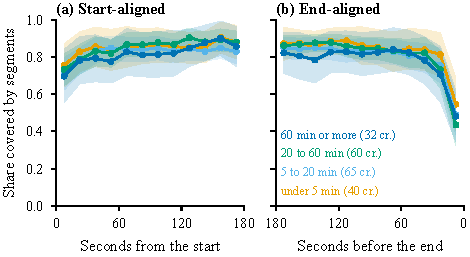
\includegraphics[width=\columnwidth]{floats/fig_coverage.pdf}
\caption{Share of each 15-s bin inside recognizer segments (filter version 2), aligned at the start (top) and at the
end (bottom) of the recording, by length band, \NSeen{} seen creators weighted equally. Grey: sup-$t$ simultaneous 95\%
band from creator-then-recording resamples; dotted: pointwise 95\%; dashed: all lengths; axis 0 to 1; bins under 5
creators omitted. Seen creators only: no positional display of the hold-out is drawn.}
\label{fig:coverage}
\end{figure}

\begin{figure}[ht]
\centering
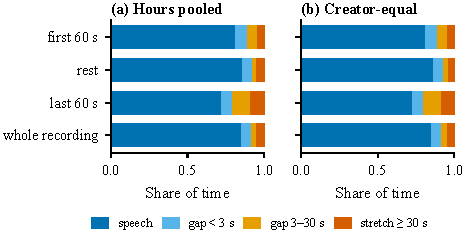
\includegraphics[width=\columnwidth]{floats/fig_classes.pdf}
\caption{Running time inside recognizer segments, in gaps under 3\,s, in gaps of 3--30\,s and in stretches of 30\,s or
more (filter version 2), for the whole recording, the first 60\,s, the rest and the last 60\,s; (a) hours pooled, (b)
creators weighted equally, with 95\% creator-bootstrap intervals; \NSeen{} seen creators. Music, meditation and silence
cannot be told apart.}
\label{fig:classes}
\end{figure}

\begin{table*}[tp]
\centering
\small
% tab_nonspeech.tex: GENERATED by the private builder build_numbers.py at 2026-11-26T03:59:48Z; label tab:nonspeech. The writer adds the float,
% the caption and the label. Sources: a private file of the run (named in the private build record)
% Seen creators; percentages of audio time.
{\scriptsize\setlength{\tabcolsep}{2pt}
\begin{tabular}{@{}p{0.34\textwidth}rlll@{}}
\toprule
Definition & Hours & Pooled \% [95\%] & Creator-equal \% [$t$ 95\%] & Creator median \% [95\%] \\
\midrule
voice detector's non-speech (audio minus detector speech seconds) & 66.4 & 12.1 [7.7, 17.5] & 12.2 [8.7, 15.6] & 7.9 [5.3, 10.9] \\
time outside recognizer segments, artefact filter v2 & 81.3 & 14.8 [10.9, 19.9] & 14.9 [11.8, 18.0] & 11.4 [9.6, 12.9] \\
time outside recognizer segments, no filter & 81.1 & 14.8 [10.9, 19.9] & 14.9 [11.8, 17.9] & 11.4 [9.5, 12.9] \\
of which before the first or after the last segment (filter v2) & 24.4 & 4.4 [1.2, 9.8] & 3.8 [1.2, 6.4] & 0.8 [0.5, 1.3] \\
\midrule
\multicolumn{5}{@{}p{0.97\linewidth}}{\emph{Coverage by recognizer segments (filter v2), creator-equal [95\%]}} \\
last partial decoding window (creator-equal) &  & 0.48 [0.41, 0.54] & 71 cr. & 1{,}208 rec. \\
full 30-s window before it (creator-equal) &  & 0.78 [0.73, 0.82] & 71 cr. & 1{,}208 rec. \\
difference, last partial minus window before &  & \ensuremath{-}0.30 [\ensuremath{-}0.35, \ensuremath{-}0.26] & 71 cr. & 1{,}208 rec. \\
middle: 180 s from the start to 180 s before the end, recordings of 6 min or more (creator-equal) &  & 0.87 [0.85, 0.90] & all but $<$5 cr. & 1{,}053 rec. \\
last 15 s (all lengths) &  & 0.49 [0.42, 0.55] & 71 cr. & 1{,}293 rec. \\
15 to 30 s before the end (all lengths) &  & 0.77 [0.71, 0.82] & 71 cr. & 1{,}293 rec. \\
first 15 s (all lengths) &  & 0.75 [0.70, 0.80] & 71 cr. & 1{,}293 rec. \\
\midrule
\multicolumn{5}{@{}p{0.97\linewidth}}{Segment-gap share minus detector share per recording: median 3.5 points (P10 -2.4, P90 6.9); Spearman 0.89} \\
\bottomrule
\end{tabular}}

\caption{Share of audio without speech, seen creators: the voice detector's non-speech and time outside recognizer
segments (filter version 2 and none), pooled over hours, creator-equal and at the creator median, with 95\% intervals and
leave-one-creator-out ranges; and the coverage of the last partial decoding window against the window before it.}
\label{tab:nonspeech}
\end{table*}

\paragraph{Variance and error tolerance.} Moved here from Section 5.7 by the page limit (results round): the caption
anchor's creator mean has a 95\% $t$ bound up to \AnchorCaptionMeanTHi\% and is \AnchorCaptionPooledPct\% pooled, so the
tolerance thresholds lie near either form of the measured machine disagreement; error that differs between creators
can link word length, MATTR-1000 and filled pauses to the share without speech, so their between-creator comparisons
carry a caveat. Figure~\ref{fig:icc} shows the share of variance between creators for each
measure, and Table~\ref{tab:vp} is the full variance partition behind it; Figure~\ref{fig:tolerance} and
Table~\ref{tab:tolerance} give the error tolerance of the word measures (Section~\ref{sec:variance}). Tolerance is not
accuracy. Moved here from Section 5.7 by the page limit: error that differs between creators and tracks non-speech can
move their creator-level correlation with non-speech share by up to \RSixAssocMax{} either way (word length, MATTR-1000)
and \RSixFillerAssoc{} (filled pauses) at a 10\% median; pronoun, contraction, question-mark and numeral rates, pace and
log words keep their structure. Every between-creator comparison of word length, MATTR or filled-pause rate carries this
caveat. The MATTR window is 500 words for the ICC, 1,000 in the tolerance and 100 in the bridge (``variety'').
Gaussian and logit ICC intervals rest on \VpDrawsGauss{} creator draws. Moved here from Section 5.7 by the page limit
(fourth review round): the ANOVA estimate of the earlier draft for mean segment log-probability is \IccSegLogpAnova{}
(\IccSegLogpAnovaLo--\IccSegLogpAnovaHi); negative-binomial intervals rest on \VpDrawsNb{} creator draws; parametric
intervals are \ParamNarrowLo{} to \ParamNarrowHi{} times narrower for \ParamNarrowRows{} of the \VpMeasures{} measures;
for first-person singular the point values are \IccFsRaw{} (raw) and \IccFsLog{} (log), an illustration of scale, and
\IccFs{} on the latent scale (95\% \IccFsLo--\IccFsHi).

% INTEGRATOR: moved here from Section 5.7 by the P7 move log (build of 2026-11-21 07:05 UTC); caption unchanged.
\begin{figure}[tp]
\centering
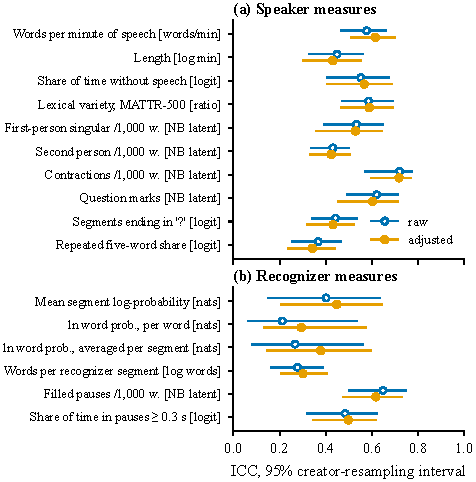
\includegraphics[width=\columnwidth]{floats/fig_icc.pdf}
\caption{Share of variance between creators (ICC) for word and timing measures (a) and recognizer measures (b), on
\VpCreators{} seen creators and \VpRecordings{} recordings (filter version 2), each on the scale named in its label: raw
(open) and adjusted for log length, edition and median word probability (filled), with 95\% creator-resampling
intervals; grey bars: parametric intervals, for comparison only. A design fact of this roster.}
\label{fig:icc}
\end{figure}

\begin{table*}[tp]
\centering
\small
% tab_vp.tex: GENERATED by WORK/build_numbers.py at 2026-11-22T01:51:42Z; label tab:vp. The writer adds the float,
% the caption and the label. Sources: REV/build-robustness/out/R5/R5-VP1-variance-partition.csv
% CB: creator-resampling bootstrap; CB/PB: width of the creator bootstrap over the parametric interval.
{\scriptsize\setlength{\tabcolsep}{2.5pt}
\begin{tabular}{@{}p{0.2\textwidth}p{0.11\textwidth}llrlrrrr@{}}
\toprule
Measure & Scale & Panel & ICC raw [95\% CB] & CB/PB & Adjusted [95\% CB] & Filter off & Kish deff & $n_{\mathrm{eff}}$ & $R_{10}$ \\
\midrule
Words per minute of speech & identity (words/min) & speaker & 0.58 [0.47, 0.66] & 1.1 & 0.62 [0.51, 0.70] & 0.59 & 10.6 & 114 & 0.93 \\
Length & log minutes & speaker & 0.45 [0.33, 0.56] & 1.3 & 0.43 [0.30, 0.55] & 0.45 & 8.5 & 143 & 0.89 \\
Share of time without speech & logit of share & speaker & 0.55 [0.41, 0.67] & 1.5 & 0.57 [0.41, 0.68] & 0.55 & 10.2 & 119 & 0.93 \\
Lexical variety & identity (ratio) & speaker & 0.59 [0.47, 0.69] & 1.2 & 0.59 [0.47, 0.69] & 0.58 & 10.3 & 107 & 0.93 \\
First-person singular per 1,000 words & NB latent log-rate & speaker & 0.53 [0.40, 0.65] & 1.4 & 0.53 [0.36, 0.64] & 0.53 & 9.9 & 123 & 0.92 \\
Second person per 1,000 words & NB latent log-rate & speaker & 0.43 [0.34, 0.50] & 0.9 & 0.42 [0.33, 0.50] & 0.43 & 8.2 & 148 & 0.88 \\
Contractions per 1,000 words & NB latent log-rate & speaker & 0.72 [0.57, 0.77] & 1.3 & 0.72 [0.60, 0.77] & 0.72 & 13.0 & 93 & 0.96 \\
Question marks per 1,000 words & NB latent log-rate & speaker & 0.62 [0.49, 0.71] & 1.2 & 0.60 [0.46, 0.71] & 0.62 & 11.3 & 107 & 0.94 \\
Segments ending in '?' & logit of share & speaker & 0.44 [0.34, 0.53] & 1.1 & 0.43 [0.32, 0.52] & 0.44 & 8.4 & 145 & 0.89 \\
Repeated five-word share & logit of share & speaker & 0.37 [0.26, 0.46] & 1.2 & 0.34 [0.24, 0.44] & 0.37 & 7.1 & 170 & 0.85 \\
Mean segment log-probability & identity (nats) & recognizer & 0.40 [0.15, 0.63] & 2.7 & 0.45 [0.21, 0.64] & 0.40 & 7.7 & 157 & 0.87 \\
Mean ln word probability, per word & identity (nats) & recognizer & 0.21 [0.06, 0.53] & 3.6 & 0.29 [0.13, 0.57] & 0.22 & 4.5 & 268 & 0.73 \\
Mean ln word probability, averaged per segment & identity (nats) & recognizer & 0.27 [0.08, 0.56] & 3.0 & 0.38 [0.15, 0.59] & 0.27 & 5.5 & 222 & 0.79 \\
Words per recognizer segment & log words & recognizer & 0.28 [0.16, 0.39] & 1.4 & 0.30 [0.21, 0.40] & 0.28 & 5.6 & 215 & 0.79 \\
Filled pauses per 1,000 words & NB latent log-rate & recognizer & 0.65 [0.50, 0.75] & 1.2 & 0.62 [0.47, 0.73] & 0.65 & 11.8 & 103 & 0.95 \\
Share of time in pauses $\geq$ 0.3 s & logit of share & recognizer & 0.48 [0.32, 0.62] & 1.6 & 0.50 [0.35, 0.62] & 0.47 & 9.1 & 133 & 0.90 \\
\bottomrule
\end{tabular}}

\caption{Table VP-1, condensed: measure, scale, raw ICC with its 95\% creator-resampling interval, adjusted ICC (log
length, edition, median word probability), ICC with the filter off, Kish design effect, effective recordings and the
reliability of a ten-recording creator mean; \VpCreators{} seen creators, \VpRecordings{} recordings, filter version 2.
The ICC is a design fact of this roster.}
\label{tab:vp}
\end{table*}

\begin{figure*}[tp]
\centering
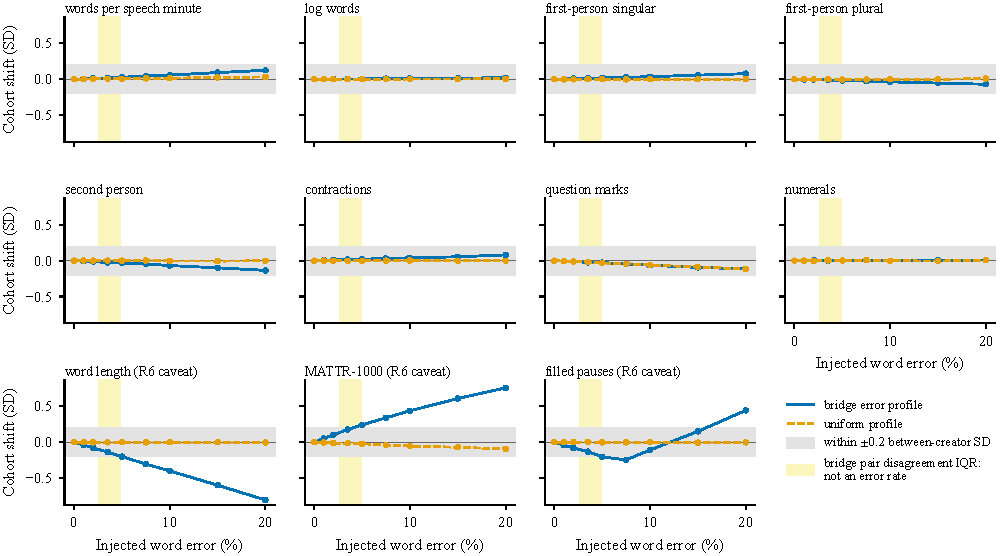
\includegraphics[width=\textwidth]{floats/fig_tolerance.pdf}
\caption{Injected word error (0--20\%) against each word measure's creator-equal cohort mean relative to its clean
value, with the bridge's edit profile (solid) and a uniform profile (dashed); grey: 10th--90th percentile over creators;
dotted: $\pm$0.2 between-creator SD. The vertical band marks the bridge's model-to-model disagreement, which is not an
error rate. Tolerance, not accuracy.}
\label{fig:tolerance}
\end{figure*}

\begin{table}[ht]
\centering
\small
% tab_tolerance.tex: GENERATED by WORK/build_numbers.py at 2026-11-22T01:51:42Z; label tab:tolerance. The writer adds the float,
% the caption and the label. Sources: REV/build-robustness/out/R6/R6-tolerance-table.csv; REV/build-robustness/out/R6/R6-creator-error-scenarios.csv
% First three columns: injected error (per cent, bridge profile, same rate for every creator) at which the cohort mean, the median creator and the 90th-percentile creator move 0.2 between-creator SD. Last three: creator-differing error (sigma 0.86, rho 0.7 with non-speech share) at a 3.5% median: Spearman of creator means with the clean ones, and change of the creator-level correlation with non-speech share at 3.5% and 10% medians.
{\scriptsize\setlength{\tabcolsep}{2pt}
\begin{tabular}{@{}p{0.2\linewidth}rrrrrrrr@{}}
\toprule
Measure & Coh. & Med. & P90 & 3.5\% & ICC$_{20}$ & $\rho$ & $\Delta\rho_{3.5}$ & $\Delta\rho_{10}$ \\
\midrule
log words & $>$20 & $>$20 & $>$20 & 0.00 & 0.45 & 1.00 & 0.00 & 0.01 \\
words per speech minute & $>$20 & $>$20 & $>$20 & 0.02 & 0.58 & 1.00 & 0.02 & 0.04 \\
mean word length (letters) & 5.0 & 5.2 & 3.8 & \ensuremath{-}0.14 & 0.57 & 0.92 & \ensuremath{-}0.16 & \ensuremath{-}0.27 \\
MATTR (1,000) & 4.0 & 4.2 & 3.2 & 0.18 & 0.64 & 0.91 & 0.18 & 0.26 \\
contractions /1,000 & $>$20 & $>$20 & 14.1 & 0.02 & 0.60 & 1.00 & 0.03 & 0.05 \\
first-person singular /1,000 & $>$20 & $>$20 & 13.4 & 0.01 & 0.28 & 1.00 & 0.00 & 0.02 \\
first-person plural /1,000 & $>$20 & $>$20 & 19.9 & \ensuremath{-}0.01 & 0.37 & 1.00 & 0.00 & 0.00 \\
second person /1,000 & $>$20 & $>$20 & 14.6 & \ensuremath{-}0.03 & 0.43 & 1.00 & \ensuremath{-}0.02 & \ensuremath{-}0.04 \\
question marks /1,000 & $>$20 & $>$20 & 17.8 & \ensuremath{-}0.02 & 0.30 & 1.00 & 0.00 & \ensuremath{-}0.01 \\
filled pauses /1,000 & 4.9 & 4.7 & 1.1 & \ensuremath{-}0.13 & 0.01 & 0.71 & 0.18 & 0.43 \\
numerals /1,000 & $>$20 & $>$20 & $>$20 & 0.00 & 0.25 & 1.00 & 0.01 & 0.01 \\
\bottomrule
\end{tabular}}

\caption{Injected error rate at which the cohort mean, the median creator and the 90th-percentile creator move by 0.2
between-creator SD, by edit profile, with the same rate for every creator; and the scenarios in which the error rate
differs between creators and tracks pace or the share of time without speech. ICC$_{20}$ is the ICC at 20\% injected
error, a simulation summary without interval. Between-creator comparisons of word length, MATTR and filled-pause rate
carry the caveat of Section~\ref{sec:variance}.}
\label{tab:tolerance}
\end{table}

\paragraph{Bridge.} Table~\ref{tab:bridge-verdicts} gives the bridge verdicts under both scales and both kinds of
interval (Section~\ref{sec:bridge}). The figure of mean paired differences and the Bland--Altman summaries of earlier
drafts are not printed (fourth review round): beside the registered bridge results, the seen pairs' means, intervals
and limits of agreement would give single pairs' values by difference, and a bin median of a fifth of the pairs is one
pair's value.

\begin{table}[ht]
\centering
\small
% tab_bridge_verdicts.tex: GENERATED by WORK/build_numbers.py at 2026-11-22T01:51:42Z; label tab:bridge-verdicts. The writer adds the float,
% the caption and the label. Sources: REV/build-robustness/out/R3/R3-bridge-verdicts.csv
% The seen pairs (all but fewer than 5 of the registered pairs, one per creator; their count is not printed); margin +/-0.2 SD; verdicts only (round 4: no seen-pair mean, interval or limit of agreement, no drop column). Each verdict equals the verdict on all registered pairs; no single-pair drop moves a verdict between agrees and differs.
{\scriptsize\setlength{\tabcolsep}{3pt}
\begin{tabular}{@{}p{0.40\linewidth}llll@{}}
\toprule
Measure & Between & Betw.\ sim. & Within & With.\ sim. \\
\midrule
Contracted forms /1,000 & agrees & agrees & agrees & agrees \\
Distinct words in 100-word windows & agrees & agrees & agrees & agrees \\
First-person plural /1,000 & agrees & agrees & agrees & agrees \\
First-person singular /1,000 & agrees & agrees & agrees & agrees \\
Mean word length (letters) & agrees & agrees & agrees & open \\
Second person /1,000 & agrees & agrees & agrees & agrees \\
Words per minute of speech & agrees & agrees & agrees & agrees \\
Isolated short segments, per hour & open & open & open & open \\
Loop words removed /1,000 & open & open & agrees & agrees \\
Mean word probability & open & open & open & open \\
Thanks phrase removed, per hour & open & open & open & open \\
Filled pauses /1,000 & differs & differs & differs & differs \\
Mean word duration (s) & differs & differs & differs & differs \\
Pauses 0.3-1 s per speech minute & differs & differs & differs & differs \\
Pauses $\geq$ 1 s per speech minute & differs & differs & differs & differs \\
Share of time in pauses $\geq$ 0.3 s & differs & differs & differs & differs \\
Words per recognizer segment & differs & differs & differs & open \\
\bottomrule
\end{tabular}}

\caption{Bridge verdicts per measure on the between-creator (Between) and the within-creator scale (Within), with
per-measure and simultaneous (sim.) 90\% $t$ intervals against the margin of $\pm$\BridgeMargin{} SD fixed in advance, on \BridgeSeenPairs{} seen pairs
(all but fewer than 5 of its \BridgePairs{} registered pairs); verdicts only, each equal to the verdict on all registered pairs. No single-pair drop moves a verdict between agrees and differs. The verdicts concern means over English
audio of 5--60 minutes, not single recordings or other languages; neither transcript is a human reference.}
\label{tab:bridge-verdicts}
\end{table}

\paragraph{Weighting and window sensitivity.} Figure~\ref{fig:sensitivity} and Table~\ref{tab:sensitivity} show each
headline under other weightings and windows, against a margin fixed before the run.

\begin{figure*}[tp]
\centering
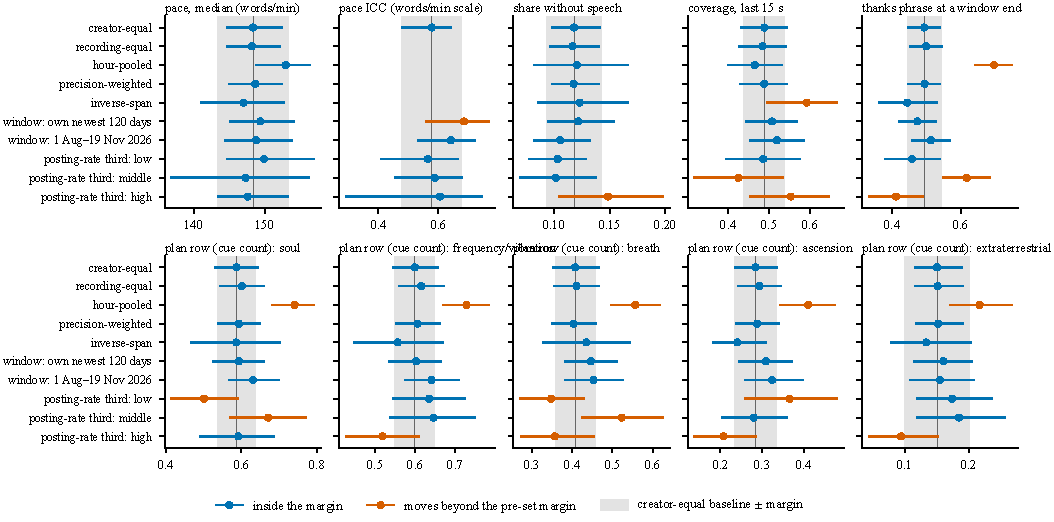
\includegraphics[width=\textwidth]{floats/fig_sensitivity.pdf}
\caption{Headline numbers, and the reporting plan's cue-count robustness rows (``plan row''), under five weightings and
three restrictions (each creator's own newest 120 days, a fixed calendar window, thirds of posting rate), with
creator-bootstrap 90\% intervals; grey band: the creator-equal baseline $\pm$ the margin fixed before the run. In this
roster, under the newest-20 quota; no period or trend.}
\label{fig:sensitivity}
\end{figure*}

\begin{table*}[tp]
\centering
\small
% tab_sensitivity.tex: GENERATED by WORK/build_numbers.py at 2026-11-22T00:15:32Z; label tab:sensitivity. The writer adds the float,
% the caption and the label. Sources: REV/build-robustness/out/R4/R4-summary-table.csv
{\scriptsize\setlength{\tabcolsep}{2.5pt}
\begin{tabular}{@{}p{0.2\textwidth}rrlllp{0.33\textwidth}@{}}
\toprule
Headline & Baseline & Margin & Range & Beyond margin & Interval outside & Largest mover \\
\midrule
pace, median (words/min) & 148.4 & 5.0 & 146.6--153.6 & 2 of 40 & 0 & hour-pooled / own newest 120 days / none / all \\
pace, ICC & 0.578 & 0.100 & 0.565--0.685 & 1 of 6 & 0 & creator-equal / own newest 120 days / none / all \\
share without speech & 0.118 & 0.025 & 0.102--0.148 & 3 of 40 & 0 & creator-equal / all / none / high \\
speech coverage, last 15 s & 0.489 & 0.050 & 0.425--0.604 & 9 of 40 & 0 & inverse-span / calendar 2026-08-01 to 2026-11-19 / none / all \\
thanks phrase at a window end & 0.494 & 0.050 & 0.411--0.705 & 20 of 40 & 8 & hour-pooled / all / 5 min / all \\
robustness row of the plan (cue count, not a headline): cue share: soul & 0.587 & 0.050 & 0.501--0.784 & 19 of 40 & 7 & hour-pooled / calendar 2026-08-01 to 2026-11-19 / 5 min / all \\
robustness row of the plan (cue count, not a headline): cue share: frequency/vibration & 0.599 & 0.050 & 0.518--0.734 & 14 of 40 & 5 & hour-pooled / all / 5 min / all \\
robustness row of the plan (cue count, not a headline): cue share: breath & 0.408 & 0.050 & 0.348--0.576 & 15 of 40 & 7 & hour-pooled / own newest 120 days / 5 min / all \\
robustness row of the plan (cue count, not a headline): cue share: ascension & 0.285 & 0.050 & 0.208--0.415 & 9 of 40 & 3 & hour-pooled / all / 5 min / all \\
robustness row of the plan (cue count, not a headline): cue share: extraterrestrial/alien & 0.150 & 0.050 & 0.094--0.219 & 6 of 40 & 0 & hour-pooled / all / 5 min / all \\
\bottomrule
\end{tabular}}

\caption{Per headline: creator-equal baseline, the margin fixed before the run, the range over the \RFourSpecs{}
specifications, and how many move the estimate beyond the margin. Baselines are the sensitivity build's own
creator-equal estimates and can differ in the last digit from the figures of Section~\ref{sec:measure}. The term rows
are robustness rows of the reporting plan (cue counts), not headlines of this paper and not findings about channelling.}
\label{tab:sensitivity}
\end{table*}

\paragraph{Model-coded checks of the measurement.} Table~\ref{tab:kinds} is the interim census of recording kinds
(Section~\ref{sec:data}), Table~\ref{tab:nonlanguage} the pseudo-word flag (Section~\ref{sec:pipeline}) and
Table~\ref{tab:labelflips} how much the choice of recognizer moves model-coded labels. All three are model-coded and not
checked by a person.

\begin{table}[ht]
\centering
\small
% tab_kinds.tex: GENERATED by the private builder build_numbers.py at 2026-11-26T03:59:48Z; label tab:kinds. The writer adds the float,
% the caption and the label. Sources: a private file of the run (named in the private build record)
% Interim, model-coded, not checked by a person; development creators only; creator-weighted. Every kind and band holds 5 or more creators (checked with small_cells.pool_small_groups).
{\scriptsize\setlength{\tabcolsep}{2pt}
\begin{tabular}{@{}p{0.3\linewidth}llllr@{}}
\toprule
Kind (largest by words) & $n$ (S / M) & Rec.\ S \% [95\%] & Rec.\ M \% [95\%] & Agr. & Stab. \\
\midrule
Channelled (embodied) voice & 25 / 28 & 26 [17, 37] & 29 [20, 39] & 0.79 & 0.98 \\
Relayed message & 11 / 7 & 12 [4, 21] & 7 [2, 15] & 0.78 & 0.96 \\
Interview or podcast & 14 / 13 & 15 [7, 23] & 14 [6, 22] & 0.81 & 0.99 \\
Guided practice & 10 / 11 & 10 [4, 18] & 11 [5, 19] & 0.95 & 1.00 \\
Own-voice talk & 31 / 32 & 32 [22, 43] & 33 [24, 43] & 0.89 & 0.95 \\
Advert or other & 5 / 5 & 5 [1, 9] & 5 [1, 10] & 0.80 & 0.96 \\
\midrule
Main kind channelled or relayed & 36 / 35 & 38 [26, 49] & 37 [26, 47] & 0.85 & -- \\
\midrule
Claimed voice in any part & 70 / 59 & 73 [63, 84] & 62 [50, 73] & 0.90 & 0.91 \\
Claimed voice in 10\%+ of words & 50 / 48 & 52 [41, 64] & 50 [38, 62] & 0.88 & 0.93 \\
Claimed voice in 25\%+ of words & 43 / 40 & 45 [34, 56] & 42 [31, 52] & 0.87 & 0.94 \\
\midrule
\multicolumn{6}{@{}p{0.97\linewidth}}{\emph{Claimed-voice band of a recording, creator-weighted \% [95\%], small / middle}} \\
0 & 26 / 37 & 27 [16, 37] & 38 [27, 50] &  &  \\
under 10 & 20 / 11 & 21 [13, 30] & 12 [4, 20] &  &  \\
10 to 25 & 7 / 8 & 7 [2, 13] & 8 [2, 16] &  &  \\
25 to 50 & 12 / 10 & 13 [6, 20] & 11 [4, 18] &  &  \\
50 or more & 31 / 30 & 32 [22, 43] & 31 [22, 42] &  &  \\
\bottomrule
\end{tabular}}

\caption{Interim census of recording kinds and claimed-voice bands on \LOneRecordings{} recordings of \LOneCreators{}
development creators: creator-weighted shares of recordings and of speech hours with 95\% creator-bootstrap intervals,
under the small model (modal kind of five runs) and the middle model, with their specific agreement and run-to-run
stability. Model-coded, not checked by a person; development creators only; interim. It replaces the earlier draft's
count from a purposive reading.}
\label{tab:kinds}
\end{table}

\begin{table}[ht]
\centering
\small
% tab_nonlanguage.tex: GENERATED by the private builder build_numbers.py at 2026-11-26T03:59:48Z; label tab:nonlanguage. The writer adds the float,
% the caption and the label. Sources: a private file of the run (named in the private build record)
% Model-read (both model tiers agree), not checked by a person; window level with creator bootstrap. Lower block: with / without flagged windows.
{\scriptsize\setlength{\tabcolsep}{2pt}
\begin{tabular}{@{}p{0.11\linewidth}p{0.17\linewidth}rrp{0.16\linewidth}p{0.16\linewidth}@{}}
\toprule
Sample & Creators & Windows & Cr. & Coherent language [95\%] & Non-language [95\%] \\
\midrule
flagged & all seen & 200 & 56 & 0.38\newline[0.24, 0.67] & 0.51\newline[0.19, 0.68] \\
flagged & development & 147 & 42 & 0.52\newline[0.31, 0.79] & 0.36\newline[0.08, 0.61] \\
flagged & check & 53 & 14 & 0.21\newline[0.10, 0.77] & 0.70\newline[0.19, 0.88] \\
unflagged & all seen & 200 & 71 & 1.00\newline[1.00, 1.00] & 0.00\newline[0.00, 0.00] \\
unflagged & development & 135 & 48 & 1.00\newline[1.00, 1.00] & 0.00\newline[0.00, 0.00] \\
unflagged & check & 65 & 23 & 1.00\newline[1.00, 1.00] & 0.00\newline[0.00, 0.00] \\
\midrule
\multicolumn{6}{@{}p{0.97\linewidth}}{\emph{Lexical measures with and without flagged windows (creator means [95\%])}} \\
MATTR &  &  & 71 & 0.647\newline[0.640, 0.655] & 0.647\newline[0.640, 0.655] \\
types per 1,000 words &  &  & all but $<$5 & 338.8\newline[330.6, 347.1] & 338.4\newline[330.1, 346.5] \\
words per minute &  &  & 71 & 148.6\newline[144.7, 152.4] & 148.9\newline[145.0, 152.8] \\
names per 1,000 words &  &  & 71 & 2.749\newline[2.175, 3.403] & 2.744\newline[2.170, 3.393] \\
\bottomrule
\end{tabular}}

\caption{Pseudo-word flag, fixed on development creators before any reading: model-read share of flagged and unflagged
30-s windows read as non-language, weighted to all windows of each stratum, and lexical measures with and without the
flagged windows. Model-read: without audio a reader cannot tell glossolalia from misrecognised speech or another
language.}
\label{tab:nonlanguage}
\end{table}

\begin{table}[ht]
\centering
\small
% tab_labelflips.tex: GENERATED by WORK/build_numbers.py at 2026-11-22T00:15:32Z; label tab:labelflips. The writer adds the float,
% the caption and the label. Sources: REV/build-llm/out/L2/tab-L2-label-flips.csv; REV/build-llm/out/L2/L2-summary.json
% Model-coded; rows the L2 build marks as shown (enough recordings). Rec.: bridge recordings of development creators, one per creator; a count fewer than 5 below a count it is nested in is printed as 'all but <5'.
{\scriptsize\setlength{\tabcolsep}{2pt}
\begin{tabular}{@{}lp{0.24\linewidth}lrp{0.14\linewidth}p{0.14\linewidth}p{0.14\linewidth}@{}}
\toprule
Instr. & Label & Unit & Rec. & Between transcripts [90\%] & Run to run [90\%] & Difference [90\%] \\
\midrule
voice & all labels (share of words) & words & 25 & 0.19\newline[0.10, 0.28] & 0.22\newline[0.13, 0.31] & \ensuremath{-}0.02\newline[\ensuremath{-}0.08, 0.02] \\
voice & claimed voice (V2 or V3) (1 - Jaccard) & words & 16 & 0.21\newline[0.11, 0.36] & 0.27\newline[0.13, 0.48] & \ensuremath{-}0.06\newline[\ensuremath{-}0.14, 0.02] \\
voice & claimed or not (share of all words) & words & 16 & 0.07\newline[0.04, 0.11] & 0.09\newline[0.04, 0.15] & \ensuremath{-}0.02\newline[\ensuremath{-}0.06, 0.01] \\
voice & V1 own person (1 - Jaccard) & words & all but $<$5 & 0.23\newline[0.11, 0.36] & 0.25\newline[0.12, 0.40] & \ensuremath{-}0.02\newline[\ensuremath{-}0.07, 0.02] \\
voice & V2 embodied source (1 - Jaccard) & words & 10 & 0.11\newline[0.01, 0.26] & 0.21\newline[0.01, 0.49] & \ensuremath{-}0.10\newline[\ensuremath{-}0.23, 0.01] \\
voice & V3 relayed source (1 - Jaccard) & words & 11 & 0.54\newline[0.37, 0.86] & 0.68\newline[0.42, 0.98] & \ensuremath{-}0.13\newline[\ensuremath{-}0.24, 0.00] \\
voice & V4 other participant (1 - Jaccard) & words & 8 & 0.74\newline[0.27, 0.85] & 0.61\newline[0.30, 0.73] & 0.13\newline[\ensuremath{-}0.06, 0.17] \\
voice & V0 cannot tell (1 - Jaccard) & words & 9 & 0.47\newline[0.28, 0.70] & 0.85\newline[0.47, 0.99] & \ensuremath{-}0.38\newline[\ensuremath{-}0.48, \ensuremath{-}0.14] \\
asks & any ask & half & all but $<$5 & 0.25\newline[0.16, 0.34] & 0.15\newline[0.05, 0.26] & 0.10\newline[0.01, 0.19] \\
asks & K1 pay or enrol & half & 13 & 0.35\newline[0.20, 0.51] & 0.16\newline[0.03, 0.33] & 0.19\newline[0.07, 0.32] \\
asks & K3 platform engagement & half & 15 & 0.27\newline[0.09, 0.51] & 0.21\newline[0.00, 0.47] & 0.06\newline[\ensuremath{-}0.11, 0.30] \\
asks & K4 off-platform move & half & 11 & 0.34\newline[0.19, 0.60] & 0.17\newline[0.00, 0.29] & 0.17\newline[\ensuremath{-}0.03, 0.53] \\
asks & any ask & any & all but $<$5 & 0.22\newline[0.14, 0.30] & 0.15\newline[0.05, 0.26] & 0.07\newline[\ensuremath{-}0.01, 0.14] \\
asks & K1 pay or enrol & any & 13 & 0.35\newline[0.20, 0.51] & 0.16\newline[0.03, 0.33] & 0.19\newline[0.07, 0.32] \\
asks & K3 platform engagement & any & 15 & 0.19\newline[0.04, 0.39] & 0.21\newline[0.00, 0.47] & \ensuremath{-}0.02\newline[\ensuremath{-}0.16, 0.17] \\
asks & K4 off-platform move & any & 11 & 0.34\newline[0.19, 0.60] & 0.17\newline[0.00, 0.29] & 0.17\newline[\ensuremath{-}0.03, 0.53] \\
\bottomrule
\end{tabular}}

\caption{Stability of model-coded labels across the two recognizers' transcripts on the bridge recordings of
development creators: flip shares of voice labels (words) and asks (events) between transcripts against run-to-run
flips on one transcript, with creator-bootstrap 90\% intervals. Rec.: recordings with the label, one per creator; a
count fewer than 5 below a count it is nested in reads ``all but $<$5''. The instruments are those of that run, before
their later revisions. Stability, not accuracy.}
\label{tab:labelflips}
\end{table}

\paragraph{Exclusions.} Table~\ref{tab:exclusions} states, for each recording outside the analysed set, its likely
effect on each estimand of this paper. Live streams, short videos, paid material, other platforms and deleted recordings
were never listed, so they are not counted.

\begin{table*}[tp]
\centering
\footnotesize
\setlength{\tabcolsep}{3pt}
\begin{tabular}{@{}>{\raggedright\arraybackslash}p{0.12\textwidth}>{\raggedright\arraybackslash}p{0.10\textwidth}%
>{\raggedright\arraybackslash}p{0.12\textwidth}>{\raggedright\arraybackslash}p{0.10\textwidth}%
>{\raggedright\arraybackslash}p{0.11\textwidth}>{\raggedright\arraybackslash}p{0.13\textwidth}%
>{\raggedright\arraybackslash}p{0.12\textwidth}>{\raggedright\arraybackslash}p{0.10\textwidth}@{}}
\toprule
Exclusion & Size & Time without speech & Artefacts & Coverage & Voice & Asks & Forecasts \\
\midrule
Live streams & not listed & unknown & more windows per recording & outside the quota & interactive channelled sessions under-represented & asks to a live audience under-represented & unknown \\
Short videos & not listed & unknown & few windows & outside the quota & excerpts of sessions missing & promotional asks may be missing & unknown \\
Members-only and paid material & not listed & unknown & unknown & outside the quota & full sessions behind payment missing & asks measured on the free tier only & unknown \\
Other platforms & not listed & unknown & unknown & publisher editions used as audio only & unknown & unknown & unknown \\
Deleted before the listing & not observable & unknown & unknown & not observable & unknown & unknown & forecasts that failed may be missing (survivorship) \\
Set aside before the run (English text of another kind, or a language review) & \NSetAside{} recordings (other text: \NOtherTextCreators{} creators) & newest ranks missing from run measures & newest ranks missing & newest ranks under-represented (Section~\ref{sec:coverage}) & newest ranks missing & newest ranks missing & newest ranks missing \\
Final download failures & \NFailed{} recordings, \NFailedCreators{} creators & missing recordings shorter on average (Table~\ref{tab:rank-odds}) & small & small & small & small & small \\
Not transcribed & \NNotTranscribed{} recordings, most without speech & files without speech left out, so the share without speech is slightly understated & none & small & none & none & none \\
\bottomrule
\end{tabular}
\caption{Exclusions and their likely effect on each estimand of this paper. ``Not listed'': outside the newest-20 listing
of regular public uploads, so not counted. Directions are judgments from the design, not measurements, except where a
section or table is named.}
\label{tab:exclusions}
\end{table*}

\paragraph{Entrance cues and two-level correlations.} Table~\ref{tab:entry} reports the entrance experiment's cue counts
under its first frozen version, the version of record, with its revision beside it. Table~\ref{tab:cor} gives
correlations between delivery and recognizer confidence at two levels, which replaces the earlier draft's pooled
statement.

\begin{table}[ht]
\centering
\small
% tab_entry.tex: GENERATED by WORK/build_numbers.py at 2026-11-22T00:15:32Z; label tab:entry. The writer adds the float,
% the caption and the label. Sources: R2R/ENTRY/out/v1-2026-11-21/entry-e4-how-common.csv; R2R/ENTRY/out/entry-read-precision.csv; R2R/ENTRY/out/entry-t3-v1-v2.csv
% Seen creators; cue counts and upper bounds; one reading by a model, not a person. Bins merged with small_cells.merge_small_bins.
{\scriptsize\setlength{\tabcolsep}{3pt}
\begin{tabular}{@{}p{0.55\linewidth}ll@{}}
\toprule
Row & Count & Share [interval] \\
\midrule
\multicolumn{3}{@{}p{0.97\linewidth}}{\emph{Version 1 (primary, frozen before the check reading): read precision, Wilson 95\%}} \\
check (after freeze): first entrance: a source speaks at the cue & 7 of 14 & 0.50 [0.27, 0.73] \\
check (after freeze): first entrance: on target and at the opening of the source's speech & n.p. & $<$5 creators \\
development (in-sample): first entrance: a source speaks at the cue & 33 of 34 & 0.97 [0.85, 0.99] \\
\midrule
\multicolumn{3}{@{}p{0.97\linewidth}}{\emph{Creators by share of their recordings with a first entrance cue (bins of 5 or more creators; cue counts, upper bounds)}} \\
none & 40 creators &  \\
0--10\% & 14 creators &  \\
10--20\% & 8 creators &  \\
20--100\% & 9 creators &  \\
creator-balanced share of recordings with an entrance cue (90\%) &  & 0.09 [0.05, 0.12] \\
person of the entrance cue: I (singular) (share of cues, creator-balanced, 90\%) &  & 0.63 [0.49, 0.77] \\
person of the entrance cue: we (plural) (share of cues, creator-balanced, 90\%) &  & 0.37 [0.23, 0.51] \\
\midrule
\multicolumn{3}{@{}p{0.97\linewidth}}{\emph{Version 2 (revised after the check reading; secondary row)}} \\
recordings with a first entrance cue & v1 108 & v2 94 \\
creators with a first entrance cue & v1 31 & v2 25 \\
\bottomrule
\end{tabular}}

\caption{Entrance cues, version 1 (frozen before the check reading; version of record): read precision with Wilson
95\% intervals; distribution over creators of the share of recordings with a first-entrance cue, in bins of 5 or more
creators; the creator-balanced share of recordings with a cue and the person of the cue, with 90\% creator-then-recording
intervals; version 2 (revised after a model check) as a revision row of counts. On check creators \EntryReadOn{} of
\EntryRead{} cues were on target, as read once by a model agent and not checked by a person; a share whose on-target
items come from fewer than 5 creators is not printed (n.p.). Cue counts and upper bounds.}
\label{tab:entry}
\end{table}

\begin{table}[ht]
\centering
\small
% tab_cor.tex: GENERATED by WORK/build_numbers.py at 2026-11-22T00:15:32Z; label tab:cor. The writer adds the float,
% the caption and the label. Sources: R2R/TOPICS/out/COR/cor-f24-confidence-delivery.csv; REV/build-descriptive/out/D4/D4-table-U.csv
% Spearman on creator means (71 seen creators) and within creators (ranks inside each creator; creators with 5+ recordings, all but fewer than 5 of the seen); 90% creator bootstrap. Last row: D4 Table U, its own definitions and 95% intervals.
{\scriptsize\setlength{\tabcolsep}{3pt}
\begin{tabular}{@{}p{0.4\linewidth}ll@{}}
\toprule
Pair & Between creators [90\%] & Within creators [90\%] \\
\midrule
mean word log-probability -- pace & 0.11 [\ensuremath{-}0.09, 0.31] & 0.10 [0.04, 0.17] \\
mean word log-probability -- share without speech & \ensuremath{-}0.19 [\ensuremath{-}0.39, 0.01] & \ensuremath{-}0.07 [\ensuremath{-}0.13, \ensuremath{-}0.01] \\
mean word log-probability -- log words & \ensuremath{-}0.12 [\ensuremath{-}0.30, 0.07] & \ensuremath{-}0.09 [\ensuremath{-}0.16, \ensuremath{-}0.03] \\
pace -- share without speech & \ensuremath{-}0.37 [\ensuremath{-}0.54, \ensuremath{-}0.18] & \ensuremath{-}0.34 [\ensuremath{-}0.40, \ensuremath{-}0.27] \\
pace -- log words & 0.24 [0.03, 0.43] & 0.26 [0.19, 0.32] \\
share without speech -- log words & \ensuremath{-}0.43 [\ensuremath{-}0.59, \ensuremath{-}0.25] & \ensuremath{-}0.23 [\ensuremath{-}0.30, \ensuremath{-}0.16] \\
\midrule
mean segment log-probability -- pace (D4: creator medians; creator-centred values; 95\%) & 0.54 [0.35, 0.69] & 0.43 [0.36, 0.50] \\
\bottomrule
\end{tabular}}

\caption{Spearman correlations of pace, the share of time without speech, log words and mean log word probability (a
stand-in for recognizer confidence) at two levels: between creators (creator means) and within creators (ranks inside
each creator, for creators with 5 or more recordings; primary), with 90\% creator-bootstrap intervals. Last row: the
earlier draft's pooled correlation of mean segment log-probability with pace, split at two levels in Table U with that
table's own definitions (creator medians; creator-centred values) and 95\% intervals: \CorSegLogpPaceBetween{} between
and \CorSegLogpPaceWithin{} within creators.}
\label{tab:cor}
\end{table}

\clearpage
% sections/appendix-protocol.tex -- Appendix B, protocol records.
% Writer: C. Written 2026-11-21, 06:13 to 06:25 UTC (clock: date -u). Prose about 735 words, captions about 890
%   (appendix, outside the 8-page budget).
% Floats: tab:freeze, tab:gates, tab:ka, tab:doubleread, tab:crossvendor, tab:hthree, fig:hthree, fig:eligibility,
%   fig:power, fig:plasmode, tab:deviations, fig:timeline, tab:contacts, tab:outputs.
%   Table bodies floats/tab_*.tex are expected to hold the tabular only (caption and label are here).
%   Figures floats/fig_*.pdf are copied or re-drawn by build_floats.py (fig_hthree.pdf holds the placebo and the trim
%   panel of R1, side by side or stacked).
% Fourth review round (from 12:50 UTC; clock: date -u): the known-answer bounds with their assumption (methods review
%   M3); A10 "at freeze 2 at the latest" (M12); the class 'mixed' and the 02:55 merge's scope in the deviation caption
%   (M1, M11, M12); freeze 1's timing against the 03:08 rule (M6); no line at the hold-out creators with English
%   recordings (privacy review P5).
% Macros used that are not in outline section 7: \DblSUnits, \DblSCreators, \DblFcUnits, \DblFcCreators
%   (requested in findings/macros-requested-C.md).
% Results round (2026-11-21, from 19:16 UTC; clock: date -u): freeze 1's amendment, freeze 2 and its constants, A10
%   entered, first-round production and its interfaces; the 12:52 decisions (H6's window, asks counted once, H9's mask);
%   CAL part (f) not run; the first-round results tables tab:results-detail, tab:results-rows, tab:results-holm from the
%   public results file (pending until it exists); deviation and timeline captions to the registry of 18:41.
% Final pre-push check (2026-11-21, from 23:35 UTC; clock: date -u): the lead's rule of 22:33 UTC for every agreement
%   figure applied to the gate tables, the second reading and the 00:30 figures (a figure that fails reads "not
%   published (fewer than 5 creators)"); the deviation caption to the registry row of 23:34, with the class
%   'reporting' inside 'other'; the timeline caption to the latest registry row (\TimelineEndStamp).
%   Lead's decision of 2026-11-22 00:15 UTC: the rule as worded; a figure over several codes with no single positive
%   code needs 5 or more creators in all and disagreements from none or 5 or more creators (codes given alike are not
%   tested on their own); the captions and the sentence of the gates paragraph say so.
% Pre-publish verification (2026-11-21, from 21:30 UTC; clock: date -u): the committed spend with its measured part
%   (unreleased reservations of ended runs); the gate tables cover the gate sample G, with the R-hold failures
%   (\ResRholdCommit, \ResRholdSentC); the recording-property projections against the minimum only (tab:programme,
%   fig:eligibility); the hold-out median of English recordings over all hold-out creators; c of tab:ka under the
%   nested-count rule.
% Pending labels used: \PendVerDep, \PendVerAdjG, \PendHThreeX, \PendTlBuild, \PendLabV, \PendLabA, \PendLabF,
%   \PendLabS, \PendLabT, \PendLabK; the result macros and tables of findings/results.tex and floats/tab_results*.tex.
% "registry 04:59" and the like name rows of the registry dated 21 November 2026 (UTC).

\section{Protocol records}
\label{app:protocol}

This appendix holds the records behind Sections~\ref{sec:protocol} to~\ref{sec:deviations}. Every label is model-coded,
and no person checked any label (A8). Agreement between models is reliability, not validity. Exploratory (registry A2);
not a test of H1--H10, except H3's registered rows. The status tables, the programme table, the second-reading and
cross-vendor detail, the H3 detail and the paragraph on roles and versions were moved here from Sections 6 and 7 by the
page limit, unchanged except for the third review round's corrections (move log of that round).

\paragraph{Measurement status.} Tables~\ref{tab:status} and~\ref{tab:status-labels} give each construct's instrument,
reference, reliability, bridge verdict, grid sensitivity and the uses allowed in this paper.

% INTEGRATOR (2026-11-21): the status table is taller than a page, so the builder writes it in two parts; the second
% part (the model-coded label instruments) has no bridge or seam column because every such cell is empty.
\begin{table*}[tp]
\centering
\small
% tab_status.tex: GENERATED by the private builder build_numbers.py at 2026-11-26T03:59:48Z; label tab:status. The writer adds the float,
% the caption and the label. Sources: a private file of the run (named in the private build record); PUB/findings/numbers.tex
% Part 1 of 2 (transcript and audio measures). D5 rows updated with WER, BR-GS, GRID, gates, KA, VER-3R and second-reading figures; every update is logged in the private build record (d5-updates.csv). Reference 'model' or 'none': no accuracy claim is possible.
{\scriptsize\setlength{\tabcolsep}{2pt}
\begin{tabular}{@{}p{0.09\textwidth}p{0.13\textwidth}p{0.06\textwidth}p{0.24\textwidth}p{0.13\textwidth}p{0.14\textwidth}p{0.15\textwidth}@{}}
\toprule
Construct & Instrument and version & Reference & Reliability (n, interval; source) & Bridge (two models) & Seam sensitivity & Allowed uses \\
\midrule
pace (words per minute of speech) & word count / voice-detector speech minutes; recognizer english-only distil model (run 2026-11-20) & none & ICC 0.58 [0.47, 0.66] words/min, 71 creators (R5) & agrees (seen pairs) & word counts move \ensuremath{-}0.18\% under a 15-s grid shift (BR-GS) & registered tests and seen-derived constants: English-only model only (recognizer rule, registry 03:08); across both models only descriptively, on average, for English audio of 5--60 min (bridge) \\
pauses (gaps between words) & word time stamps of the recognizer & none & ICC 0.48 [0.32, 0.62] logit (R5) & differs (seen pairs); long pauses: differs (seen pairs) & grid makes 3.0\% of gaps 0.3--30 s (GRID); shift moves pause share \ensuremath{-}0.14 points (BR-GS); capped seam rule (registry 03:08) & within one model only, with and without the seam rule; never across languages \\
word duration & word time stamps & none & none measured & differs (seen pairs) & not measured & within one model only; descriptive \\
fillers (um, uh) & closed token list on recognizer words & none & ICC 0.65 [0.50, 0.75] NB latent (R5); R6 caveat & differs (seen pairs) & 7.7\% above flat in a window's last 3 s (GRID) & within one model only; never as a speaker trait \\
pronoun rates (1sg, 1pl, 2nd) & closed lists on recognizer words & rule & 1sg ICC 0.53 [0.40, 0.65] NB latent (R5) & agrees (seen pairs); 1pl and 2nd agree (bridge verdict table) & not affected & within English; cue counts per 1,000 words; recording or creator level \\
contractions & closed list (prep.py contraction table, H4 list) & rule & ICC 0.72 [0.57, 0.77] NB latent (R5) & agrees (seen pairs) & not affected & within English; descriptive \\
lexical variety & MATTR-500 (descriptives); MATTR-100 in the bridge & none & MATTR-500 ICC 0.59 [0.47, 0.69] ratio (R5); R6 caveat & agrees (seen pairs) & not affected & within English; with length band \\
names & NAMES private variant list (model-adjudicated, 2,843 candidates) and dispersion rule & model & mask leak: exact-stem matching found 64\% of mentions of six public families (F19) & -- & -- & masking only; no counts of named beings in this paper \\
years and numbers & rx-norm-v1 normalisation + rx-patterns-v1 & model & model-read precision of the digit-date pattern D6 0.81 (Wilson 95\% from RXP; 59 hits read) & -- & -- & cue counts \\
language of a recording & multilingual model probes; creator rule; fallback (setup) & model (metadata agrees for 144 files) & none; 78.2\% of decisions by the creator rule & not applicable & -- & description; language means its few creators (R11) \\
speech time (share without speech) & voice detector of the recognizer (min silence 500 ms) & none & ICC 0.55 [0.41, 0.67] logit (R5); two definitions agree per recording, Spearman 0.89 (D3) & not applicable & -- & `the voice detector's non-speech': pooled 12.1\%, creator-equal 12.2\%, creator median 7.9\% (D3) \\
artefact rules (filter v2) & artefact\_filter\_v2.py (5 rules) & rule (model agents' reading of 42 transcripts) & positional thanks rule: its share bound from window-phase counts (GRID) not published (misses not recounted by creator); isolated rule: at least 62.5\% grid-tied; no listening & open (artefact and confidence rates not settled by the seen pairs) & the rules are defined on the grid & every number states its filter version (raw, version 1 or version 2) \\
\bottomrule
\end{tabular}}

\caption{Measurement status per construct, part 1, transcript and audio measures: instrument and version; reference
(none, rule, model or machine text); reliability with $n$ and interval; bridge verdict (two recognizer models);
decoding-grid sensitivity; uses allowed in this paper. Updated from the paper review's status table with the agreement
anchors, the grid shift, the gates, the known-answer battery, the cross-vendor reader and the second reading; every
update is logged. No row is checked by a person; agreement between machines is not accuracy.}
\label{tab:status}
\end{table*}

\begin{table*}[tp]
\centering
\small
% tab_status_labels.tex: GENERATED by WORK/build_numbers.py at 2026-11-22T01:51:42Z; label tab:status-labels. The writer adds the float,
% the caption and the label. Sources: REV/build-descriptive/out/D5/D5-measurement-status.csv; PUB/findings/numbers.tex
% Part 2 of 2 (model-coded label instruments; bridge and seam cells are all '--' and are not printed). D5 rows updated with WER, BR-GS, GRID, gates, KA, VER-3R and second-reading figures; every update is logged in WORK/d5-updates.csv. Reference 'model' or 'none': no accuracy claim is possible.
{\scriptsize\setlength{\tabcolsep}{2pt}
\begin{tabular}{@{}p{0.12\textwidth}p{0.17\textwidth}p{0.07\textwidth}p{0.4\textwidth}p{0.2\textwidth}@{}}
\toprule
Construct & Instrument and version & Reference & Reliability (n, interval; source) & Allowed uses \\
\midrule
voice span (claimed against own) & voice instrument (LLM, two tiers), frozen at freeze 1 & model & rev.~3 gate C 0.901, gate D $\kappa$ 0.890 (relayed row fails, 0.762 [0.488]); cross-vendor $\kappa$ 0.91 [0.84, 0.95] (VG-6, weighted; unweighted 0.63); known-answer relayed passages recovered, small model: 0.74 on rev.~2, 0.89 on rev.~3; middle 0.91--1.00 on rev.~3 arms & model-coded; relayed merged into claimed after the relayed row and the pre-declared merge failed (02:55; looser than the letter of plan 3.4); `responds to punctuation and case' \\
ask (pay or enrol) & asks instrument (LLM) & model & gate C 0.795 [0.667], gate D 0.867; middle check is the record; known-answer found 0.98, non-asks kept 0.01 & model-coded \\
forecast parts (class, time window) & forecast instrument (LLM) + TIME rule rows & model and rule & critic gate D 0.64 [0.503] (one revision); checkability gate D fails (named actor 0.38); second reading, time window $\kappa$ 0.70 [0.55, 0.92]; known-answer parts 0.88--1.00 & model-coded; below floor where gates failed (owner, 00:30); F1 against the rest is the class of record \\
commitment (hedges) & forecast instrument hedge code; RX hedge patterns & model & hedge kappa 0.60 (F39); model-read precision lexical hedge 0.84, modal hedge 0.67 (RXP) & model-coded; cue counts \\
sentence group (world claim, practice) & content instrument (LLM) & model & second reading $\kappa$ 0.79 [0.73, 0.83], 400 units; known-answer at ceiling & model-coded \\
title group (presentation, voiced-by) & title instrument (LLM) & model & failed gates of record on G: presentation $\kappa$ 0.64 [0.53, 0.74] (floor 0.70), stability (floor 0.90) not published (fewer than 5 creators); at the owner's 00:30 decision both figures not published (fewer than 5 creators); large model decides disputes & model-coded; presentation only \\
\bottomrule
\end{tabular}}

\caption{Measurement status per construct, part 2, model-coded label instruments (columns as in part 1; neither the
bridge nor the decoding grid was measured for them). Gate figures are the gates of record on the gate sample, with the
registry's figures at the owner's 00:30 decision beside them where they differ. Every label is model-coded and not
checked by a person.}
\label{tab:status-labels}
\end{table*}

\paragraph{Roles, timeline and versions.} Labels come from the OpenAI models; Anthropic model agents were the
cross-vendor reader, the panels, proposers and skeptic, and the drafters of this paper (full list in the ethics
statement). The labelling method is ``guided steps'': typed fields before the label. The prediction timeline reports
what was predicted and whether an outcome is observable, never whether it came true (\PendTlBuild); sources outside the
selection rule (deceased persons, a higher self) are separate rows. A first frozen
version stays the version of record and revisions are rows, as for the entrance patterns (Table~\ref{tab:entry}).

\paragraph{Freezes and gates.} Freeze 1 fixes the instruments (Table~\ref{tab:freeze}; record prefix \FreezeOnePrefix).
Freeze 1 did not wait for the last known-answer voice batches, which cannot change an instrument whose one revision is
spent (registry 04:59), against the 03:08 rule that it wait for the battery (looser for its timing); they finished at
09:10. Seen production ran \ProdSeenStamp{} and measured \ProdSeenUsd{} USD; committed spend then stood at
\ProdCommittedUsd{} USD (registry 11:10), under the 130 USD hard stop, tested at worst case with every open batch job at
its full cost (04:55). Moved here from Section 6.1 by the page limit: when the small model's batch queue returned almost
nothing, its stages moved to the standard interface with request ids and bodies unchanged (06:33 to 08:33).

\paragraph{Freeze 2 and first-round production.} Moved here from Section 6.1 by the page limit (results round). The
amendment of freeze 1 (\FreezeOneAmendStamp; record prefix \FreezeOneAmendPrefix) changed the production driver alone,
from \ProduceOldPrefix{} to \ProduceNewPrefix: a feature step that runs only after freeze 2 for a group other than the
seen one and loads the analysis package's feature code only at the hash freeze 2 pins, with the seen run's pinned
inputs, so that seen and hold-out features come from one source; every other hash, the configuration and the
request-id fixture (\FixtureRequests{} requests with equal ids and bodies) are unchanged, and the record of
\FreezeOneStamp{} is kept beside it. Freeze 2 (\FreezeTwoStamp; record prefix \FreezeTwoPrefix; registry commit
\FreezeTwoCommit, which holds A10) pins \FreezeTwoModules{} analysis modules, the constants (prefix \ConstantsPrefix) and
\FreezeTwoPinned{} files, every seen label and feature file among them. The constants came from the seen labels through
the seen-only path at \ConstantsStamp, confirmed by a second reader that imports nothing from the package. H4's
yardstick is \HFourYardstick{} over \HFourYardstickCreators{} seen creators with at least \HFourMinForms{} own-voice
forms, a minimum set in code before any seen label existed and kept, as a stated choice, once both values were known
(\HFourYardstickNoMin{} over \HFourYardstickNoMinCreators{} creators without it; the middle model's
\HFourYardstickMiddle{} beside it); the yardstick scales H4's standardised drops, so it moves the conditions that compare
a drop with 0.5 and not the sign-flip $p$. H2's length bands are \HTwoBandLo{} and \HTwoBandHi{} words, and its retained
parts the time window, named actor and observable outcome (place, \HTwoPlacePct\%, and quantity, \HTwoQuantityPct\%,
fall below the 5\% line). H9's smallest effect stays at the registry's placeholder, \HNineSesoi{} standardised units:
no rule for setting it from seen creators was registered, and one chosen with the seen cells computed would let seen
data pick the threshold; the seen H9 contrast is a description only (16:06). The Mantel-Haenszel intervals stay the
wider of two, since the coverage repeat did not run, and H6's registered half-count version stays uncentred under the
guard, with a null mean of \HSixRegNullMean{} on seen creators (15:14).

Hold-out production (\HoldoutProdStamp; \HoldoutProdRecordings{} English recordings, projected at about
\HoldoutProdProjUsd{} USD before sending) went through the standard interface, because the small model's batch queue
still returned nothing to a probe (13:23); the hard stop, tested at worst case, refused a standard-interface chunk of
the hold-out voice labels at \HardStopRefusalStamp{} (\HardStopRefusalCommitted{} USD committed plus
\HardStopRefusalWorst{} at worst case), so the middle model's voice labels went through batch, whose reservations hold
the expected cost; committed spend passed the owner's 120 USD warning at the end of hold-out production
(\WarningPassedCommitted{} USD). The other group was labelled for exploratory use. R-hold, \RholdRecordings{} hold-out
recordings, \RholdPerThird{} from each third of the run order, was drawn from ledger fields only (\RholdDrawnStamp). In
plan mode the reliability driver fed placeholder answers into the arms that reuse production's answers, so their stitched
maps and request ids differed, and it refused R-hold (\PlanModeRefusedStamp); the fix, which touches plan mode only, is
kept as a patch and not applied, the driver restored byte for byte to its frozen hash (\ReliabilityPrefix) at
\ReliabilityRestoredStamp, and R-hold ran in run mode, which rebuilds production's requests exactly (checked on every
seen recording), with per-command run limits; only the cost preview of plan mode is lost (17:29). Its small-model arms
ran through the standard interface (\RholdSmallUsd{} USD, to \RholdSmallStamp), its middle-model arms through batch for
one arm and then the standard interface, the open batch job cancelled and collected first (18:17): \RholdArms{} arms,
\RholdUsd{} USD, to \RholdDoneStamp. The large model reread \ChkHoldoutStatements{} hold-out statements for checkability
(\ChkHoldoutStamp). All labelling ended at \LabellingDoneStamp{}: \FinalCommitted{} USD committed (\SpendMeasured{}
measured, the rest held by unreleased reservations of ended runs), \FinalPastWarning{} past the warning and
\FinalBelowStop{} below the hard stop. Not bought: HR (a),
whose \HrAUsd{} USD would have left less than 1 USD under the hard stop at worst case (18:17), and HR (b, c), a
fifth-tier line that starts only while committed spend plus its cap stays within 120 USD (03:08); the rewording arms of
HR were not run.

\paragraph{Gates.} Table~\ref{tab:gates} lists
every gate on the gate sample G; the R-hold gates (A10.5) are in the public results file, and their two failures are
stated in Section~\ref{sec:instruments}. Voice, asks and the forecast critic each spent the one revision plan 3.4 allows after the gates on the gate
sample; checkability and titles had failed after both prompt revisions of the pilot stage when the owner kept them
(about 00:30). The merges plan 3.4 declares in advance (moved here from Section 6.3): unseparated conversation into
other participant; frame-only relay reported apart; a failing checkability part leaves the score; fewer than four
passing parts leave the time-window part only. Embodied against own voice gave
\VoiceGateDEmbodied{} at gate D. The ask find spent its revision on a union of two draws (gate C \AsksGateC{}
[\AsksGateCLower]); the middle ask check, exact on \AsksMiddleExact{} of \AsksMiddleExact{} quotations, is the record,
and the small check is the second reader of gate D (specific agreement \AsksGateD). The forecast critic spent its
revision on one sentence about relayed forecasts; gate D then passes (\FbGateD{} [\FbGateDLower]), ``forecast or not''
is the class of record (gate C \FbGateC), and the ten-class label fails stability against 0.85 and is description
only; its stability figure is \FbTenClassStab. Checkability fails gate D on all five parts between the small and middle
models (named actor \FcNamedActorSmallMid); against the large model four parts pass and quantity fails (the place and
named-actor figures rest on fewer than 5 creators and are not published); the quantity figure is \FcQuantityLarge. When
the owner kept checkability and titles below their floors (about 00:30, registry), the time window stood at
\ChkTimeKappaEarly{} against 0.60; the place figure of then is \ChkPlaceKappaEarly; title presentation on the check
creators: \TitlePresKappa; title stability: \TitleStab. The gates of record on the gate sample give presentation
\TitlePresKappaG{} [\TitlePresKappaGLo, \TitlePresKappaGHi] against \TitlePresFloor; stability fails its floor of
\TitleStabGFloor{} (Table~\ref{tab:gates-b}), and its figure is \TitleStabG. An agreement figure of the gate tables is
printed only where its positive code comes from 5 or more creators in each reading (a figure over several codes: 5 or
more creators in all) and its disagreements, if any, from 5 or more creators (the lead's rule of 22:33 UTC). On G the
sentence codes and the commitment code pass their gates; on R-hold the commitment code passes (\ResRholdCommit) and the
sentence codes fail gate C (\ResRholdSentC).

\begin{table}[t]
\centering
\small
% tab_freeze.tex: GENERATED by WORK/build_numbers.py at 2026-11-22T01:51:42Z; label tab:freeze. The writer adds the float,
% the caption and the label. Sources: LLM/freeze-20261121T045822Z.json; LLM/freeze.json; LLM/freeze2.json; REG/registry.md
% Tiers: small, middle, large as named in the Models row.
{\scriptsize\setlength{\tabcolsep}{2pt}
\begin{tabular}{@{}p{0.18\linewidth}p{0.5\linewidth}p{0.27\linewidth}@{}}
\toprule
Item & Value & Record model \\
\midrule
Frozen at & 2026-11-21T04:58:22Z &  \\
Record hash (prefix) & c3b1161d & registry freeze-1 table \\
Config hash (prefix) & d95387a4 &  \\
File hashes & 128 &  \\
Models & small gpt-6-luna, middle gpt-6.1-terra, large gpt-6-sol &  \\
\midrule
Voice & map small (effort low); labels small and middle; caps map 3837, label 4329; variant B & record: seen small, holdout middle, other middle \\
Asks & find small x 2 draws (effort low); check small and middle; caps find 1671, check 3449 & record: seen middle, holdout middle, other middle \\
Forecasts FA & small (effort none), cap 4000 &  \\
Forecasts FB & small (effort none), cap 700, second middle & record: seen small, holdout small, other small \\
Forecasts FC & middle (effort none), cap 800, second small & record: seen middle, holdout middle, other middle \\
Forecasts FD & small (effort none), cap 700 &  \\
Forecasts FE & small (effort none), cap 900 &  \\
Forecasts FC check & large (effort low), cap 2500 &  \\
Sentence codes & small (effort none), cap 500 & record: seen small, holdout small, other small \\
Titles & T middle (effort low); second small; TA large decides disputes & record: seen middle, holdout middle, other middle \\
\midrule
Freeze 1, amendment 1 & 16:06 UTC; record prefix c57e64db; produce.py 60bd9f62 to 0497c5b5 (the feature step, run only after freeze 2 for a group other than seen); every other hash and the config unchanged & record of 04:58 kept beside it \\
Freeze 2 & 16:10 UTC; record prefix 5ef43dd8; registry commit 941a556 (A10 entered); 22 analysis modules; constants prefix cf544528; 6{,}542 pinned files (seen labels and features included) & unlocks hold-out labels and the tests \\
\bottomrule
\end{tabular}}

\caption{Freeze 1 (instruments), recorded \FreezeOneStamp: record hash prefix, \FreezeOneFiles{} file hashes,
configuration hash prefix \FreezeOneConfigPrefix, models (small \ModelSmall, middle \ModelMiddle, large \ModelLarge),
record model per instrument and group, efforts and output caps; the last rows give the amendment of freeze 1
(\FreezeOneAmendStamp) and freeze 2 (\FreezeTwoShort; analysis constants, analysis code, the registry commit holding A10).}
\label{tab:freeze}
\end{table}

% INTEGRATOR (2026-11-21): the gate table is taller than a page; the builder writes it in two parts.
\begin{table*}[tp]
\centering
\small
% tab_gates.tex: GENERATED by WORK/build_numbers.py at 2026-11-22T00:15:32Z; label tab:gates. The writer adds the float,
% the caption and the label. Sources: LLM/pilot2/rev3-g-stats.json; LLM/pilot2/asks-gate-g-revised.json; LLM/design/fb-relayed-fix-done.md; LLM/design/gates-forecasts-content-titles-G.md; REG/registry.md; WORK/agreement-recount-g.private.json
% Part 1 of 2. Every gate on the gate sample G as recorded, failures included (the R-hold gates, A10.5, are in the public results file). Floors: combined rule (point at the floor, lower 90% bound at the floor minus 0.10) where a bound is given. Large-model figures of the forecast gates used gpt-6.2-sol; production adjudication uses gpt-6-sol. An agreement figure (gates C, D, E and the large model's re-reading) is printed only where its positive code comes from 5 or more creators in each reading (a figure over several codes: 5 or more creators in all) and the creators with an item the readings code differently are none or 5 or more (the rule of 2026-11-21 22:33 UTC as worded); its verdict is kept.
{\scriptsize\setlength{\tabcolsep}{2.5pt}
\begin{tabular}{@{}lp{0.42\textwidth}lll@{}}
\toprule
Gate & Measure & Value [90\%] & Floor [bound] & Verdict \\
\midrule
\multicolumn{5}{@{}p{0.97\linewidth}}{\emph{Voice, revision 3 (the one revision; decision 02:55 UTC)}} \\
A & valid after one repeat (every run) & 1.00 & 0.98 & pass \\
B & claimed quotations exact (pooled) & 0.983 [0.960, 0.996] & 0.95 & pass \\
C & share of words in one group over 3 runs & 0.901 [0.854, 0.942] & 0.90 & pass \\
D & claimed / own / other, small v middle, $\kappa$ & 0.890 [0.834, 0.933] & 0.60 [0.50] & pass \\
D & embodied / own / other, $\kappa$ & 0.921 [0.869, 0.954] & 0.60 [0.50] & pass \\
D & relayed voice, specific agreement & 0.762 [0.488, 0.887] & 0.60 [0.50] & \textbf{fail}: merged into claimed \\
\multicolumn{5}{@{}p{0.97\linewidth}}{\emph{Asks, after the one revision (union of two draws; decision 02:20 UTC)}} \\
A & find & 0.996 [0.989, 1.000] & 0.98 [0.88] & pass \\
A & check small & 1.000 [1.000, 1.000] & 0.98 [0.88] & pass \\
A & check middle & 1.000 [1.000, 1.000] & 0.98 [0.88] & pass \\
A & find middle model & 1.000 [1.000, 1.000] & 0.98 [0.88] & pass \\
A & check middle of the union & 1.000 [1.000, 1.000] & 0.98 [0.88] & pass \\
B & find on final asks & 0.994 [0.987, 1.000] & 0.95 [0.85] & pass \\
B & check small on its ask items & 0.913 [0.885, 0.942] & 0.95 [0.85] & \textbf{fail}: middle check is the record \\
B & check middle on its ask items & 1.000 [1.000, 1.000] & 0.95 [0.85] & pass \\
C & find K1 (in all but one run) & 0.795 [0.667, 0.902] & 0.75 [0.65] & pass \\
C & final accepted K1 (in all but one run) & not published (fewer than 5 creators) & 0.75 [0.65] & pass \\
C & find any class (in all but one run) & 0.829 [0.757, 0.901] & 0.75 [0.65] & pass \\
C & find K1 draw 0 alone (in all but one run) & 0.795 [0.667, 0.903] & 0.75 [0.65] & pass \\
D & small v middle check, specific agreement & 0.867 & 0.60 [0.50] & pass \\
E & middle-model find & 1.000 & -- & pass \\
\multicolumn{5}{@{}p{0.97\linewidth}}{\emph{Forecasts after the critic's one revision (decision 03:12 UTC); checkability: both revisions spent, kept below its floor by the owner (00:30 UTC)}} \\
A & valid after one retry, FB (chain run 1) & 0.9993 & 0.98 & pass \\
A & valid after one retry, FB gate stages (runs 2, 3; middle 300; gate E critic) & 1.000 & 0.98 & pass \\
A & valid after one retry, FC stages; FD and FE stages & 1.000 & 0.98 & pass \\
B & FB middle-model F1 statements exact & 1.000 & 0.95 & pass \\
B & FA middle-finder quotations exact & 1.000 & 0.95 & pass \\
B & FC record, non-NO parts exact (runs 1, 2, 3) & 1.000 / 1.000 / 0.995 & 0.95 & pass \\
B & FD cue quotations exact (runs 1, 2, 3) & 1.000 & 0.95 & pass \\
B & FE expression quotations exact (runs 1, 2, 3) & 1.000 & 0.95 & pass \\
C & FB statement (F1) or not, same in 3 runs & 0.93 [0.90, 0.95] & 0.85 & pass \\
C & FB class, 10 values, same in 3 runs & 0.77 [0.71, 0.81] & 0.85 & \textbf{fail} \\
C & FC record (middle): time window & 0.91 [0.84, 0.97] & 0.85 & pass \\
C & FC record: place & not published (fewer than 5 creators) & 0.85 & pass \\
C & FC record: named actor & 0.96 [0.94, 0.99] & 0.85 & pass \\
\bottomrule
\end{tabular}}

\caption{Every gate of the instruments on the gate sample G (A valid answers, B exact quotations, C stability over
three runs, D two-model agreement, E agreement with a second finder) and of the verification layer (VG), part 1: value
with 90\% interval (creators, then recordings), floor, outcome under the combined rule (point at the floor, lower bound
at the floor minus 0.10), revisions spent, the decision taken and its UTC time. Failed gates are kept. The R-hold gates
(A10.5) are in the public results file, their two failures in Section~\ref{sec:instruments}. The large model of the recorded
gates is \ModelLargeGate; production adjudication uses \ModelLarge. An agreement figure (gates C, D, E and the large
model's re-reading) is printed only where its positive code comes from 5 or more creators in each reading (a figure over
several codes: 5 or more creators in all; a code both readings give alike is not a cell of its own) and the creators
with an item the readings code differently are none or 5 or more (the lead's rule of 22:33 UTC); a figure that fails reads ``not published (fewer than 5 creators)'', its verdict kept. Counts of
valid answers are given as shares. Model-coded; agreement is not accuracy.}
\label{tab:gates}
\end{table*}

\begin{table*}[tp]
\centering
\small
% tab_gates_b.tex: GENERATED by the private builder build_numbers.py at 2026-11-26T03:59:48Z; label tab:gates. The writer adds the float,
% the caption and the label. Sources: a private file of the run (named in the private build record); REG/registry.md
% Part 2 of 2. Every gate on the gate sample G as recorded, failures included (the R-hold gates, A10.5, are in the public results file). Floors: combined rule (point at the floor, lower 90% bound at the floor minus 0.10) where a bound is given. Large-model figures of the forecast gates used gpt-6.2-sol; production adjudication uses gpt-6-sol. An agreement figure (gates C, D, E and the large model's re-reading) is printed only where its positive code comes from 5 or more creators in each reading (a figure over several codes: 5 or more creators in all) and the creators with an item the readings code differently are none or 5 or more (the rule of 2026-11-21 22:33 UTC as worded); its verdict is kept. A gate A or B share is printed only where its misses come from no creator or from 5 or more (recount by creator of 2026-11-25; a share near 100% is never printed as a bound); a share that fails reads '--' and its measure says why; its verdict is kept.
{\scriptsize\setlength{\tabcolsep}{2.5pt}
\begin{tabular}{@{}lp{0.42\textwidth}lll@{}}
\toprule
Gate & Measure & Value [90\%] & Floor [bound] & Verdict \\
\midrule
C & FC record: observable outcome & 0.96 [0.93, 0.99] & 0.85 & pass \\
C & FC record: quantity & not published (fewer than 5 creators) & 0.85 & pass \\
C & FD committed & 0.90 [0.87, 0.93] & 0.85 & pass \\
D & FB F1 or not, small vs middle, kappa & 0.64 [0.503, 0.75] & 0.60 & pass (lower bound 0.503 against 0.50) \\
D & FB F1 or not, check creators & 0.64 [0.43, 0.76] & 0.60 & \textbf{fail} \\
D & FB specific agreement on F1 & 0.71 [0.56, 0.80] &  & reported \\
D & FB class (10 values), kappa & 0.58 [0.50, 0.66] &  & reported \\
D & FC time window, record vs small (3 values) & 0.56 [0.39, 0.77] & 0.60 & \textbf{fail} \\
D & FC place & not published (fewer than 5 creators) & 0.60 & \textbf{fail} \\
D & FC named actor & 0.38 [0.13, 0.48] & 0.60 & \textbf{fail} \\
D & FC observable outcome & 0.56 [0.49, 0.71] & 0.60 & \textbf{fail} \\
D & FC quantity & not published (fewer than 5 creators) & 0.60 & \textbf{fail} \\
D & FD committed, small vs middle & 0.70 [0.64, 0.82] & 0.60 & pass \\
large & FC record vs large (weighted): time window, observable outcome; place and named actor: not published (fewer than 5 creators) & 0.73, 0.69 & 0.60 & pass (all four) \\
large & FC record vs large (weighted): quantity & not published (fewer than 5 creators) & 0.60 & \textbf{fail} \\
E & FA share recovered relative to a second finder, small finder & 0.90 [0.87, 0.94] & 0.80 & pass \\
E & gap, no hedge marker minus hedge marker & not published (fewer than 5 creators) & at most 0.10 & pass \\
\multicolumn{5}{@{}p{0.97\linewidth}}{\emph{Sentence codes (one revision, gates on G)}} \\
A & valid after one retry (runs 1, 2, 3; middle); run 1 and run 3: not published (misses from fewer than 5 creators) & -- / 1.000 / --; 1.000 & 0.98 & pass \\
B & evidence quotation exact (runs 1, 2, 3) & 0.970 / 0.972 / 0.969 & reported & reported \\
C & group of H5 (world claim, practice and feeling, neither), same in 3 runs & 0.88 [0.86, 0.90] & 0.85 & pass \\
C & primary code (12 values), same in 3 runs & 0.81 [0.79, 0.84] & none & reported \\
D & group, small vs middle, kappa & 0.80 [0.74, 0.86] & 0.60 & pass \\
D & group, check creators & 0.81 [0.73, 0.88] & 0.60 & pass \\
D & primary code, kappa & 0.67 [0.61, 0.74] & none & reported \\
\multicolumn{5}{@{}p{0.97\linewidth}}{\emph{Titles: the adjudicated form (failed after both prompt revisions allowed at the pilot stage; kept below its floors by the owner, about 00:30 UTC, at the 00:30 figures of the registry; rows here: the gate of record on G)}} \\
A & valid after one retry (middle, small, large) & 1.000 & 0.98 & pass \\
B & P1 cue quotation exact: middle / small / large / final; middle, small and final: not published (misses from fewer than 5 creators) & -- / -- / 1.000 / -- & 0.95 & pass \\
C & presentation, middle, same in 3 runs (runs 2 and 3 shuffled), 12 check creators & not published (fewer than 5 creators) & 0.90 & \textbf{fail} \\
C & source family, same in 3 runs & not published (fewer than 5 creators) & none & reported \\
D & presentation (4 codes), middle vs small, kappa & 0.64 [0.53, 0.74] & 0.70 & \textbf{fail} \\
D & source family, middle vs small, kappa & 0.74 [0.57, 0.87] & 0.60 & pass \\
D & presentation with P0 and P2 merged & 0.63 [0.49, 0.75] & 0.70 & \textbf{fail} \\
D & P1 or not & 0.70 [0.53, 0.83] & 0.70 & \textbf{fail (lower bound)} \\
D & presentation, check creators only & 0.53 [0.36, 0.68] & 0.70 & \textbf{fail} \\
D & time cue & 0.73 [0.60, 0.82] & none & reported \\
\bottomrule
\end{tabular}}

\caption{Every gate on the gate sample G, part 2 (columns as in part 1; R-hold gates in the public results file; an
agreement figure resting on fewer than 5 creators reads ``not published''). Model-coded; agreement is not accuracy.}
\label{tab:gates-b}
\end{table*}

\paragraph{Verification.} In the known-answer battery (Table~\ref{tab:ka}) the small model, on voice revision 2,
spilled the claimed label past returns to the own voice (\KaSpillE{} after embodied and \KaSpillR{} after relayed
frames, against base), handled an own offer inside a claimed passage as the known answer requires in \KaKfourVSmall,
and labelled interviews as conversation in \KaCvSixSmall{} against \KaCvSixMiddle{} for the middle model. On revision 3,
the frozen form (complete at 09:10), the spills are \KaSpillERevThree{} and \KaSpillRRevThree{} (90\%
\KaSpillRRevThreeLo{} to \KaSpillRRevThreeHi), the own-offer arm \KaKfourVSmallRevThree, the interview arm
\KaCvSixSmallRevThree{} (moved here from Section 6.4 by the page limit), the subject-change arm \KaXFourSmallRevThree{} and the
share of constructed regions matched \KaRegionsSmallRevThree{} (middle \KaRegionsMiddleRevThree); the canary gates
(VG-3) pass for voice, asks and forecasts. Planted asks are found at
\KaAsksFound{} and non-asks kept at \KaNonAsks; forecast parts are right at \KaFcPartsLo{} to \KaFcPartsHi; sentence
codes and titles are at ceiling on prototypes. The elevated and plain register arms are void by their own rule: their
rewrites, made by the labelling model's family, failed the code checks too often. Stated confidence is near ceiling, and
the small model is over-confident. After the critic's revision the bare ``they say that'' relay frame is still mostly
not a forecast of record (\KaBareFrameSmall{} and \KaBareFrameMiddle{} of \KaBareFrameN{} for the small and middle
models); the known answer was not changed afterwards. Measured cost: \KaCost{} USD.

The second reading (Table~\ref{tab:doubleread}; moved here from Section 6.4 by the page limit, results round: its
time-window disagreements mostly take the window from the period of the talk and concentrate in few creators, hence
H2's sensitivity row) set \ModelMiddle{} against the sentence-code record \ModelSmall{}
(\DblSUnits{} units, \DblSCreators{} creators) and \ModelLarge{} against the checkability record \ModelMiddle{}
(\DblFcUnits{} statements, \DblFcCreators{} creators): group kappa \DblSGroup{} (90\% \DblSGroupLo--\DblSGroupHi) and
time window \DblFcTime{} (\DblFcTimeLo--\DblFcTimeHi), moved here from Section 6.4 by the page limit. With the
general-principle code moved to world claim or to
practice and feeling, the group kappa is \DblSQTwoWorld{} or \DblSQTwoPractice; primary codes give \DblSPrimary.
Checkability: named actor \DblFcActor, observable outcome \DblFcOutcome; place \DblFcPlace; quantity \DblFcQuantity.
Commitment was not reread. Measured cost: \DblCost{} USD.

The cross-vendor reader (Table~\ref{tab:crossvendor}) gives \VtrDisagreeKappa{}
(\VtrDisagreeKappaLo--\VtrDisagreeKappaHi) on the \VtrDisagreeUnits{} units where the small and middle models' first
runs disagree; \VtrHeavyUnits{} units on which both agree that the voice is not claimed carry about
\VtrHeavySharePct\% of the weight; the bootstrap's coverage is not audited (moved here from Section 6.4 by the page
limit, results round). It saw ten units of context on each side with names masked, as the
large OpenAI model did, while the small and middle models read longer unmasked windows. Its comparator, the stored
OpenAI majority, was fixed in code before the first read; the record model's row decides nothing. Against the small
model's first run it gives \VtrSmallRunOne, against the large model \VtrLarge. The effective number of readers and the
all-same share (\PendVerDep) and a third reader on the gate samples (\PendVerAdjG) are pending.

\begin{table*}[tp]
\centering
\small
% tab_ka.tex: GENERATED by WORK/build_numbers.py at 2026-11-22T00:15:32Z; label tab:ka. The writer adds the float,
% the caption and the label. Sources: R2R/KA/out/README.md
% Part 1 of 2. Constructed texts: upper bounds; read only as differences between cells. Creator-clustered 90% bootstrap (c = creators of the constructed items; a c fewer than 5 below the largest c of its arm or block is printed against it).
{\scriptsize\setlength{\tabcolsep}{2.5pt}
\begin{tabular}{@{}lp{0.27\textwidth}ll@{}}
\toprule
Instrument & Arm and measure & Small [90\%] (n, c) & Middle / frozen form [90\%] (n, c) \\
\midrule
\multicolumn{4}{@{}p{0.97\linewidth}}{\emph{Voice, revision 3 (variant B, the frozen form): small model / middle model}} \\
voice & K1E planted claimed passages recovered (rule B) & 0.94 [0.90, 0.97] (n=934, c=30) & 0.97 [0.95, 0.99] (n=934, c=30) \\
voice & K1E embodied exact among claimed & 1.00 [1.00, 1.00] (n=886, c=30) & 1.00 [1.00, 1.00] (n=907, c=30) \\
voice & K1R planted claimed passages recovered (rule B) & 0.89 [0.82, 0.95] (n=824, c=30) & 0.93 [0.88, 0.96] (n=824, c=30) \\
voice & K1R relayed exact among claimed & 0.98 [0.96, 1.00] (n=732, c all but $<$5 of 30) & 0.99 [0.98, 1.00] (n=754, c all but $<$5 of 30) \\
voice & K1E return unit own (primary) & 0.95 [0.89, 0.99] (n=84, c=30) & 0.96 [0.92, 1.00] (n=84, c=30) \\
voice & K1R return unit own (primary) & 0.96 [0.92, 0.99] (n=86, c all but $<$5 of 30) & 0.92 [0.86, 0.98] (n=86, c all but $<$5 of 30) \\
voice & share of constructed regions matched (primary) & 0.94 [0.92, 0.95] (n=4365, c=30) & 0.96 [0.94, 0.98] (n=4365, c=30) \\
voice & constructed regions: claimed label confirmed & 0.99 [0.99, 1.00] (n=3087, c=30) & 1.00 [0.99, 1.00] (n=3223, c=30) \\
voice & K4V own offer: ask unit claimed, rule B & 0.97 [0.90, 1.00] (n=30, c=20) & 1.00 [1.00, 1.00] (n=30, c=20) \\
voice & K4V own offer: neighbours claimed, twin minus partner & 0.00 [0.00, 0.00] (n=177, c=20) & 0.00 [0.00, 0.01] (n=177, c=20) \\
voice & K4V ask without own reference: ask unit claimed & 0.84 [0.72, 0.95] (n=30, c all but $<$5 of 20) & 1.00 [1.00, 1.00] (n=30, c all but $<$5 of 20) \\
voice & X2 after farewell own (primary) & 0.88 [0.76, 0.97] (n=1369, c=18) & 0.83 [0.69, 0.95] (n=1369, c=18) \\
voice & X4 subject change: B2 claimed & 0.79 [0.66, 0.95] (n=148, c=13) & 1.00 [1.00, 1.00] (n=148, c=13) \\
voice & CV6 interview labelled V6 & 0.99 [0.98, 1.00] (n=749, c=14) & 0.91 [0.81, 1.00] (n=749, c=14) \\
voice & CVQ source claimed & 0.92 [0.82, 1.00] (n=413, c=14) & 1.00 [1.00, 1.00] (n=413, c=14) \\
voice & CVQ questioner V4 & 0.92 [0.84, 1.00] (n=59, c=14) & 1.00 [1.00, 1.00] (n=59, c=14) \\
voice & K2 cue deletion: claimed after minus before & -0.14 [-0.20, -0.09] (n=5667, c=23) & -0.04 [-0.08, -0.01] (n=5667, c=23) \\
voice & C spill after K1E frames (minus base) & -0.05 [-0.11, 0.00] (n=5363, c=30) & -0.06 [-0.11, -0.01] (n=2428, c=23) \\
voice & C spill after K1R frames (minus base) & 0.04 [-0.02, 0.09] (n=5360, c=30) & -0.02 [-0.07, 0.03] (n=2424, c=23) \\
\midrule
\multicolumn{4}{@{}p{0.97\linewidth}}{\emph{Voice, revision 2 (variant A), before the revision: small model / middle model}} \\
voice & K1E planted claimed passages recovered (rule B) & 0.98 [0.96, 1.00] (n=934, c=30) & 0.96 [0.93, 0.98] (n=934, c=30) \\
voice & K1E embodied exact among claimed & 0.99 [0.97, 1.00] (n=918, c=30) & 0.99 [0.98, 1.00] (n=893, c=30) \\
voice & K1R planted claimed passages recovered (rule B) & 0.74 [0.67, 0.81] (n=824, c=30) & 0.93 [0.89, 0.97] (n=824, c=30) \\
voice & K1R relayed exact among claimed & 0.93 [0.88, 0.97] (n=612, c all but $<$5 of 30) & 0.97 [0.93, 1.00] (n=767, c all but $<$5 of 30) \\
voice & K1E return unit own (primary) & 0.82 [0.75, 0.90] (n=84, c=30) & 0.87 [0.78, 0.94] (n=84, c=30) \\
voice & K1R return unit own (primary) & 0.93 [0.89, 0.97] (n=86, c all but $<$5 of 30) & 0.93 [0.89, 0.97] (n=86, c all but $<$5 of 30) \\
voice & share of constructed regions matched (primary) & 0.84 [0.81, 0.87] (n=4365, c=30) & 0.94 [0.91, 0.95] (n=4365, c=30) \\
voice & constructed regions: claimed label confirmed & 0.98 [0.97, 0.99] (n=2982, c=30) & 0.98 [0.96, 0.99] (n=3220, c=30) \\
\bottomrule
\end{tabular}}

\caption{Known-answer battery: share of planted answers recovered per arm by the small and the middle model, with
creator-clustered 90\% intervals. If constructed texts are easier than speech (not tested), recovery shares are upper
bounds for the corpus and error shares (spill, non-asks kept, losses after cue deletion) lower bounds; the levels are
printed, but only differences between cells are interpreted. Voice rows on revision 3, the frozen form, then on revision 2,
on the same items. $n$: items; $c$: creators of the constructed items, stated against the largest $c$ of its arm or
block (``all but $<$5'') when it falls fewer than 5 short of it. Void arms are marked. Model-coded; not checked by a person.}
\label{tab:ka}
\end{table*}

\begin{table*}[tp]
\centering
\small
% tab_ka_b.tex: GENERATED by the private builder build_numbers.py at 2026-11-26T03:59:48Z; label tab:ka. The writer adds the float,
% the caption and the label. Sources: a private file of the run (named in the private build record)
% Part 2 of 2. Constructed texts: upper bounds; read only as differences between cells. Creator-clustered 90% bootstrap (c = creators of the constructed items; a c fewer than 5 below the largest c of its arm or block is printed against it). A share is printed only where its misses come from no creator or from 5 or more, a rate of false keeps only where its non-zero values come from none or 5 or more (recount by creator of 2026-11-25); the spill, K2 and twin rows are differences between cells.
{\scriptsize\setlength{\tabcolsep}{2.5pt}
\begin{tabular}{@{}lp{0.25\textwidth}ll@{}}
\toprule
Instrument & Arm and measure & Small [90\%] (n, c) & Middle / frozen form [90\%] (n, c) \\
\midrule
voice & K4V own offer: ask unit claimed, rule B & 0.60 [0.43, 0.76] (n=30, c=20) & 1.00 [1.00, 1.00] (n=30, c=20) \\
voice & K4V own offer: neighbours claimed, twin minus partner & -0.13 [-0.24, -0.04] (n=177, c=20) & 0.00 [0.00, 0.00] (n=177, c=20) \\
voice & K4V ask without own reference: ask unit claimed & 0.59 [0.42, 0.76] (n=30, c all but $<$5 of 20) & not published (misses from fewer than 5 creators) \\
voice & X2 after farewell own (primary) & 0.83 [0.69, 0.95] (n=1369, c=18) & 0.81 [0.66, 0.93] (n=1369, c=18) \\
voice & X4 subject change: B2 claimed & not published (misses from fewer than 5 creators) & not published (misses from fewer than 5 creators) \\
voice & CV6 interview labelled V6 & 0.67 [0.54, 0.79] (n=749, c=14) & not published (misses from fewer than 5 creators) \\
voice & CVQ source claimed & 0.89 [0.81, 0.97] (n=413, c=14) & not published (misses from fewer than 5 creators) \\
voice & CVQ questioner V4 & not published (misses from fewer than 5 creators) & not published (misses from fewer than 5 creators) \\
voice & K2 cue deletion: claimed after minus before & -0.20 [-0.30, -0.10] (n=5667, c=23) & -0.04 [-0.08, -0.00] (n=5667, c=23) \\
voice & C spill after K1E frames (minus base) & 0.14 [0.06, 0.24] (n=5363, c=30) & -0.06 [-0.13, -0.01] (n=2891, c=25) \\
voice & C spill after K1R frames (minus base) & 0.18 [0.09, 0.28] (n=5360, c=30) & -0.03 [-0.07, -0.00] (n=2888, c=25) \\
voice & K3 register rewrites, elevated and plain arms & void by their own rule & void by their own rule \\
\midrule
\multicolumn{4}{@{}p{0.97\linewidth}}{\emph{Asks: round-2 check / union find (the frozen form)}} \\
asks & planted asks kept as K1 & 0.95 [0.93, 0.97] (n=400, c=41) & 0.97 [0.96, 0.98] (n=400, c=41) \\
asks & planted asks found & 0.95 [0.93, 0.97] (n=400, c=41) & 0.98 [0.97, 0.99] (n=400, c=41) \\
asks & claimed minus own context, kept K1 & 0.01 [-0.02, 0.04] (n=200, c all but $<$5 of 41) & 0.03 [0.00, 0.06] (n=200, c all but $<$5 of 41) \\
asks & planted non-asks kept as ask & not published (fewer than 5 creators with a non-zero value) & not published (fewer than 5 creators with a non-zero value) \\
asks & precision on the planted set & not published (misses from fewer than 5 creators) & not published (misses from fewer than 5 creators) \\
asks & two checks agree on planted items & 0.95 [0.91, 0.99] (n=384, c=41) & not published (misses from fewer than 5 creators) \\
\midrule
\multicolumn{4}{@{}p{0.97\linewidth}}{\emph{Forecast parts (constructed statements), share matching the constructed answer: small / middle}} \\
forecasts & time window & not published (misses from fewer than 5 creators) & not published (misses from fewer than 5 creators) \\
forecasts & place & 0.91 [0.89, 0.94] & 0.90 [0.88, 0.93] \\
forecasts & named actor & 0.95 [0.93, 0.97] & not published (misses from fewer than 5 creators) \\
forecasts & observable outcome & 0.89 [0.87, 0.91] & 0.88 [0.86, 0.90] \\
forecasts & quantity & 0.95 [0.93, 0.96] & 0.97 [0.95, 0.98] \\
sentences & primary code exact (prototypes; ceiling) & 1.00 [1.00, 1.00] & 1.00 [1.00, 1.00] \\
titles & presentation exact (ceiling) & 0.99 [0.97, 1.00] & 1.00 [0.99, 1.00] \\
\bottomrule
\end{tabular}}

\caption{Known-answer battery, part 2 (columns as in part 1).}
\label{tab:ka-b}
\end{table*}

\begin{table}[t]
\centering
\small
% tab_doubleread.tex: GENERATED by WORK/build_numbers.py at 2026-11-22T01:51:42Z; label tab:doubleread. The writer adds the float,
% the caption and the label. Sources: DBL/results.json; DBL/readings.private.json
% Seen check creators only; two models of one vendor; 90% creator-then-recording bootstrap. Model agreement is reliability, not validity. A view is printed only where its positive code comes from 5 or more creators in each reading (a view over several codes: 5 or more creators in all) and the creators with a unit the readings code differently are none or 5 or more (the rule of 2026-11-21 22:33 UTC as worded).
{\scriptsize\setlength{\tabcolsep}{2pt}
\begin{tabular}{@{}p{0.34\linewidth}rp{0.15\linewidth}p{0.15\linewidth}p{0.15\linewidth}@{}}
\toprule
View & $n$ & Share equal [90\%] & $\kappa$ [90\%] & Specific agr.\ [90\%] \\
\midrule
\multicolumn{5}{@{}p{0.97\linewidth}}{\emph{Sentence codes: record (small) against second reader (middle)}} \\
H5 group (registered grouping) & 400 & 0.86\newline[0.83, 0.90] & 0.79\newline[0.73, 0.83] & -- \\
group, Q2 to world claim & 400 & 0.83\newline[0.80, 0.86] & 0.74\newline[0.70, 0.79] & -- \\
group, Q2 to practice and feeling & 400 & 0.84\newline[0.80, 0.87] & 0.75\newline[0.69, 0.79] & -- \\
primary code (12 values) & 400 & 0.72\newline[0.68, 0.77] & 0.68\newline[0.63, 0.73] & -- \\
  world claim (one against rest) & 400 & -- & 0.84\newline[0.77, 0.90] & 0.87\newline[0.81, 0.92] \\
  practice and feeling (one against rest) & 400 & -- & 0.79\newline[0.74, 0.84] & 0.86\newline[0.81, 0.89] \\
  neither (one against rest) & 400 & -- & 0.75\newline[0.69, 0.81] & 0.87\newline[0.83, 0.90] \\
\midrule
\multicolumn{5}{@{}p{0.97\linewidth}}{\emph{Checkability parts: record (middle) against second reader (large)}} \\
time window & 300 & 0.88\newline[0.78, 0.98] & 0.70\newline[0.55, 0.92] & -- \\
place & 300 & \multicolumn{3}{l}{not published (fewer than 5 creators)} \\
named actor & 300 & 0.96\newline[0.94, 0.98] & 0.69\newline[0.55, 0.77] & -- \\
observable outcome & 300 & 0.96\newline[0.95, 0.98] & 0.79\newline[0.74, 0.86] & -- \\
quantity & 300 & \multicolumn{3}{l}{not published (fewer than 5 creators)} \\
number of YES parts & 300 & 0.80\newline[0.71, 0.89] & 0.62\newline[0.48, 0.76] & -- \\
\bottomrule
\end{tabular}}

\caption{Second reading on seen check creators: sentence groups and primary codes (record \ModelSmall, second reader
\ModelMiddle; \DblSUnits{} units) and the five checkability parts (record \ModelMiddle, second reader \ModelLarge;
\DblFcUnits{} statements): kappa and specific agreement with $n$ and 90\% interval (creators, then recordings). A view
is printed only where its positive code comes from 5 or more creators in each reading (a view over several codes: 5 or
more creators in all) and the creators with a unit the readings code differently are none or 5 or more (the lead's rule
of 22:33 UTC); place and quantity fail it and read ``not published (fewer than 5 creators)''. Two models of one vendor:
reliability, not validity.}
\label{tab:doubleread}
\end{table}

\begin{table}[t]
\centering
\small
% tab_crossvendor.tex: GENERATED by WORK/build_numbers.py at 2026-11-22T01:51:42Z; label tab:crossvendor. The writer adds the float,
% the caption and the label. Sources: V3R/private/ver-3r-report.sealed.md; PRIV/verification-timeline-2026-11-20/before-freeze/ver-3r/code/ver_3r.py
% Model-coded; no person checked any label. 200 units of 23 check creators weighted to the frame; 90% creator bootstrap, coverage not audited. Meaning of VG-6 fixed at 03:21 UTC, opened at 04:59 UTC after freeze 1.
{\scriptsize\setlength{\tabcolsep}{2pt}
\begin{tabular}{@{}p{0.44\linewidth}rllr@{}}
\toprule
Comparison & Units & Agreement & $\kappa$ [90\%] & $\kappa$ unw. \\
\midrule
\multicolumn{5}{@{}p{0.97\linewidth}}{\emph{Anthropic reader against each OpenAI reader (claimed / own / other; weighted to the frame; last column unweighted)}} \\
small run 1 (frame pair; seen record) & 200 & 91.4\% & 0.84 [0.74, 0.90] & 0.32 \\
small run 2 & 200 & 94.7\% & 0.90 [0.83, 0.94] & 0.62 \\
small run 3 & 200 & 92.6\% & 0.87 [0.76, 0.92] & 0.47 \\
small run 1, label repeat 1 & 200 & 92.4\% & 0.86 [0.76, 0.92] & 0.48 \\
small run 1, label repeat 2 & 200 & 92.0\% & 0.86 [0.75, 0.92] & 0.45 \\
middle run 1 (frame pair; hold-out record model) & 200 & 95.3\% & 0.92 [0.85, 0.95] & 0.69 \\
middle run 2 & 200 & 95.4\% & 0.92 [0.84, 0.95] & 0.69 \\
gpt-6-sol (guided steps) & 200 & 89.3\% & 0.81 [0.64, 0.93] & 0.77 \\
OpenAI majority (VG-6 comparator) & 200 & 94.9\% & 0.91 [0.84, 0.95] & 0.63 \\
three-model majority (small 1, middle 1, sol) & 192 & 96.4\% & 0.93 [0.86, 0.97] & 0.83 \\
\midrule
\multicolumn{5}{@{}p{0.97\linewidth}}{\emph{Gate VG-6: the Anthropic reader against the OpenAI majority on the collapsed contrast, kappa at least 0.60 and lower 90\% bound at least 0.50. Outcome: passes}} \\
narrow own (V1 only) for the OpenAI runs too & 200 & 94.9\% & 0.91 [0.84, 0.95] & -- \\
units the Anthropic reader called V0 left out & 194 & 95.9\% & 0.93 [0.87, 0.96] & -- \\
two classes: claimed against not claimed & 200 & 96.0\% & 0.86 [0.55, 0.93] & -- \\
claimed against own, where both say claimed or own & 105 & 96.8\% & 0.93 [0.78, 0.98] & -- \\
embodied (V2) / own / rest, against the OpenAI majority (H4) & 200 & 95.7\% & 0.91 [0.83, 0.96] & -- \\
embodied (V2) / own / rest, against gpt-6-sol & 200 & 89.9\% & 0.81 [0.62, 0.93] & -- \\
against small run 1 (frame pair; seen record) & 200 & 91.4\% & 0.84 [0.74, 0.90] & -- \\
against middle run 1 (frame pair; hold-out record model) & 200 & 95.3\% & 0.92 [0.85, 0.95] & -- \\
against three-model majority (small 1, middle 1, sol) & 192 & 96.4\% & 0.93 [0.86, 0.97] & -- \\
\midrule
\multicolumn{5}{@{}p{0.97\linewidth}}{\emph{The hard stratum of the check sample: units on which the first runs of the small and the middle model give different groups (against the OpenAI majority, weighted within the stratum; source: VER-3R sampling code)}} \\
stratum `disagree' (half of the units) & 100 & 69.9\% & 0.53 [0.21, 0.67] & -- \\
\multicolumn{5}{@{}p{0.97\linewidth}}{\emph{Weight: the 30 agree-not-claimed units carry about 73\% of the frame weight; the weighted figures rest mostly on them.}} \\
\bottomrule
\end{tabular}}

\caption{Cross-vendor check (gate VG-6) on \VtrUnits{} units of \VtrCreators{} check creators, weighted to
\VtrFrameUnits{} units of \VtrRecordings{} recordings: the Anthropic reader against each OpenAI reader and their
majority, weighted kappa with 90\% creator-bootstrap intervals (coverage not audited; such intervals covered below
nominal at \MinCreatorsRegistered{} to \HThreeCreators{} creators in this project's audit) and the unweighted kappa; the rule (kappa at least 0.60, lower
bound at least 0.50, against the stored OpenAI majority) and its outcome; sensitivity rows, which decide nothing; the
stratum where the small and middle models' first runs disagree; and where the frame weight sits. Model-coded; not
checked by a person.}
\label{tab:crossvendor}
\end{table}

\paragraph{H3 and the programme.} Table~\ref{tab:programme} is the registered programme, Table~\ref{tab:hthree} and
Figure~\ref{fig:hthree} carry Section~\ref{sec:hthree}, and Figures~\ref{fig:eligibility} to~\ref{fig:plasmode} carry
Section~\ref{sec:tests}. Moved here from Section 7 by the page limit (results round): the pilot behind the projections
holds \PilotWRecordings{} recordings of as many creators, while hold-out creators have a median of
\HoldoutEnglishRecMedian{} English recordings; the smallest attainable $p$ at the lower bound is \MinPHOne, \MinPHFour{}
and \MinPHSix{} for H1, H4 and H6; H2's power is at the nearest CAL count (\PowerHTwoCreators) and H5's at
\PowerHFiveCreators; under placebo H3's registered rule says ``supported'' in \HThreePlaceboTwelve\% of sets of
\MinCreatorsRegistered{} creators as well; the tests run as registered and amended (A10 under its guard; the 02:55
merge). H3 in detail: as arithmetic on the published hold-out summary, not as creator-level rows of the
frozen code, the 90\% $t$ interval on the \HThreeCreators{} creator means is \HThreeTLo{} to \HThreeTHi{} and
\HThreePositive{} of \HThreeCreators{} creators are positive; the seen value recentred to a null mean of zero is
\HThreeSeenRecentred{} (90\% \HThreeSeenRecentredLo{} to \HThreeSeenRecentredHi; moved here from Section 7.1 by the
page limit), with creator sign-flip $p$ \HThreeSeenSignFlipP; at sets of \MinCreatorsRegistered{} and \HThreeCreators{} creators CAL's
power at the smallest effect is \HThreePowerTwelve\% and \HThreePowerSeventeen\%, and an audit made afterwards found 90\%
coverage of \HThreeCovTwelve{} and \HThreeCovSeventeen{} (two-stage percentile) and \HThreeCovT{} ($t$). Moved here from
Section 7 by the page limit (fourth review round): the DerSimonian--Laird intervals of H1 and H4 over-reject under the
placebo too, as normal intervals do with few clusters \cite{cameron2008bootstrapbased,mackinnon2022clusterrobust};
H2 and H5 were revised at the analysis level before freeze 1, and before freeze 2 and any hold-out label the
hypothesis code was verified again (details below); the registered versions stay as registered under A10's guard.
Revisions before freeze 1, in full: H2's primary row drops statements whose checkability and commitment share scenario or
withdrawal wording (fixed rule; flagged row beside it) and keeps parts with at least 5\% prevalence; a sensitivity row
counts time windows taken only from the period of the talk as ``no''; H5 excludes units next to a self-naming cue and
reports three placements of the general-principle code; H1 and H6 use claimed voice (embodied and relayed), H4 embodied
voice; relayed-only rows carry no verdict (``below the reliability floor''). Revisions of the hypothesis code before
freeze 2 and any hold-out label, moved here from Section 7: the amended H6 version's observed-minus-expected statistic is
centred per recording (06:44); its reference became a conditional draw under the per-recording null, because the
one-sided sign-flip rejected \HSixSignFlipRejectPct\% at the 0.005 level when creators have one ask at a low claimed
share (09:19); because an ask-level conditional reference over-rejects on bursts (\HSixBurstRejectPct\% at 0.005 for
bursts of \HSixBurstSize), asks are redrawn by cluster and the larger of the cluster-level conditional $p$ and the
sign-flip $p$ enters the guard, with \HSixDraws{} draws (11:08, which also withdrew the 09:19 claim that the new
reference can only make a verdict harder to reach); H9's content words exclude the frozen family table and the
name-list forms, and contractions of function words count as function words (11:08). After the fifth verification
(12:52): asks within \HSixClusterUnits{} units of each other, about a minute of speech, chain into one cluster, with a
\HSixClusterSensUnits-unit window as a sensitivity row and dependence beyond the window not modelled; with \HSixDraws{}
draws the side of 0.005 still depends on the draws inside about \HSixPBandLo{} to \HSixPBandHi; asks of one class whose
unit ranges overlap count once, since the union of two find draws can return one ask twice (a counting correction in
both versions of H6, outside the guard; 15:14); ain't and y'all also count as function words; the wide mask stays, every
token of every family variant (about \HNineMaskPct\% of content tokens), which can only lower same-family content
similarity. CAL's re-projection of eligibility from seen labels (part f) did not run (16:06).

\begin{table*}[tp]
\centering
\small
% tab_programme.tex: GENERATED by WORK/build_numbers.py at 2026-11-22T01:51:42Z; label tab:programme. The writer adds the float,
% the caption and the label. Sources: REV/build-robustness/out/R2/R2-calibration-eligibility-table.csv; R2R/CAL/out/cal-table.json
% Min.: creators for the first Holm step / registered not-run minimum. Projected eligible hold-out creators from model-coded pilot labels: creator-property bound (median [90% range]), then (second line) recording-property bound, stated against the registered minimum only; a range end left open is not printed (the projections are capped at a count the paper withholds); H5 an upper bound from pilot titles. Power: CAL at the SESOI at the CAL creator count in brackets, for each bound. Results: macros of findings/results.tex.
{\scriptsize\setlength{\tabcolsep}{2pt}
\begin{tabular}{@{}lp{0.065\textwidth}p{0.2\textwidth}p{0.07\textwidth}lp{0.075\textwidth}p{0.06\textwidth}p{0.04\textwidth}p{0.205\textwidth}p{0.07\textwidth}@{}}
\toprule
 & State & Registered reference: CAL verdict & SESOI & Min. & Projected [90\%] & Power & Min.\ $p$ & Announcement (02:50) or projection reading; instrument & Result \\
\midrule
H1 & first round & sign-flip p passes; the registered DL interval verdict exceeds twice nominal at 8 and 12 creators: use HKSJ or t & log ratio -0.05 (5\% slower) & 8 / 12 & 5 [2--10]\newline above min. & 0.00\newline 0.51 (17) & 0.031 & announced 02:50: probably not determinable (lower bound below the registered minimum); on the creator-property bound (the recording-property bound is above the minimum); relayed voice merged into claimed after its gate failed (02:55) & \ResHOneKind \\
H2 & first round & FAILS: within-creator reference rejects about 14 times nominal; creator sign-flip is nominal & $|$D$|$ 0.10 & 9 / 8 & 16 [13--]\newline above min. & 0.51 (17)\newline 0.51 (17) & $<$0.001 & not announced; projection reads: determinable on count; \textbf{instrument below its floor} (checkability; owner's 00:30 exception, A10.5) & \ResHTwoKind \\
H3 & tested; withdrawn (A6) & FAILS: shift test 2.6 times nominal at 17 creators, 4 times at 8; estimate not centred (-0.063) & U 0.10 & 8 / -- & 17 [17--17] & 0.05 (17) & $<$0.001 & closed (A6) & withdrawn (A6); Sec.~7 \\
H4 & first round & sign-flip p passes; DL interval about 1.7 times nominal: use HKSJ or t & 0.5 between-creator SD & 8 / 12 & 3 [0--7]\newline above min. & 0.00\newline 0.92 (17) & 0.125 & announced 02:50: probably not determinable (lower bound below the registered minimum); on the creator-property bound (the recording-property bound is above the minimum); relayed voice merged into claimed after its gate failed (02:55) & \ResHFourKind \\
H5 & first round & bias small at these counts; percentile interval under-covers; needs the label-based repeat & 0.4 log units (upper-bound projection) & 8 / 12 & 11 [6--15]\newline (upper bound only) & 0.21 (12) & $<$0.001 & not announced; projection reads: probably not determinable (median below the registered minimum); \textbf{instrument below its floor} (title codes; owner's 00:30 exception, A10.5) & \ResHFiveKind \\
H6 & first round & FAILS: registered half-count rule 2.3 times nominal at 12 creators, 4 times at 17; conditional OE sign-flip near nominal & rate ratio 0.5 & 8 / 12 & 5 [1--9]\newline above min. & 0.00\newline 0.18 (17) & 0.031 & announced 02:50: probably not determinable (lower bound below the registered minimum); on the creator-property bound (the recording-property bound is above the minimum); relayed voice merged into claimed after its gate failed (02:55) & \ResHSixKind \\
H7 & not run (needs the wave) & needs the replication wave; SD item supplies the estimator, L reference and its spread & placeholder 0.01 cosine & 8 / -- & -- & -- & -- & waits for the wave & not run: needs the wave \\
H8 & dropped (A9); counted p = 1 & needs the comparison set; inherits H3's centring problem (-0.063) if the two groups differ in count regime & 0.5 SD (comparison set) & 8 / -- & -- & -- & -- & dropped (A9) & dropped (A9), $p = 1$ \\
H9 & first round & needs frozen family labels and the name list; reference is already creator-level & 0.2 standardised (placeholder) & 8 / -- & -- & -- & -- & not announced; not projected (R2): its cells need labels and the name list; smallest effect the registry's placeholder, adopted 16:06; \textbf{instrument below its floor} (title codes; owner's 00:30 exception, A10.5) & \ResHNineKind \\
H10 & not run (needs the wave) & needs the wave; run condition 50 matured statements from 15 creators & risk difference 0.15 & 9 / 15 & -- & -- & -- & run condition: 50 matured statements from 15 creators & not run: needs the wave \\
\bottomrule
\end{tabular}}

\caption{The registered programme, stated before any hold-out label: state; registered reference and CAL's verdict on
it (creator-level placebo on seen-creator analogues); smallest effect; minimum creators for the first Holm step and the
registered ``not run'' minimum; projected eligible hold-out creators (model-coded pilot labels) under CAL's
creator-property bound (median, 90\% range; an end left open would show a count this paper withholds) and its
recording-property bound (against the minimum only); H5 one upper bound, H9 not projected; CAL's power at the smallest
effect under each (CAL creator count in brackets); smallest attainable $p$ at the first bound; the 02:50 announcement
(H1, H4, H6) or the projection's reading, and instrument flags (bold: below its floor by the owner's exception, A10.5);
result (public results file). Projections, not counts.}
\label{tab:programme}
\end{table*} H7's smallest effect is still open: a multiple $k$ of the spread of its estimand under its block
reference on seen creators, with $k$ fixed before any wave recording (A10.6; H7 is not run in the first round). H9's
is the registry's placeholder, \HNineSesoi, adopted at 16:06 (a deviation). Hedge rates by kind (lexical against modal)
are a planned seen-label output beside H2's commitment code (\PendLabF).

\paragraph{First-round results.} Tables~\ref{tab:results-detail} to~\ref{tab:results-holm} carry
Section~\ref{sec:results} from the public results file that the converter writes from the private report, with every
creator count in a printed form; nothing here is read from the private report. \ResWithheld{} Supported and refuted
verdicts carry their verification figures in Table~\ref{tab:results-detail}.

\begin{table*}[tp]
\centering
\small
% tab_results_detail.tex: GENERATED by the private builder build_numbers.py at 2026-11-26T03:59:48Z; label tab:results-detail. The writer adds the float,
% the caption and the label. Sources: REG/results/first-round-2026-11-21.json
% Both versions under A10's guard, from the public results file; creator counts the paper does not print are stated against the minimum.
{\tiny\setlength{\tabcolsep}{2pt}
\begin{tabular}{@{}p{0.03\textwidth}p{0.06\textwidth}p{0.11\textwidth}p{0.06\textwidth}p{0.27\textwidth}p{0.3\textwidth}p{0.1\textwidth}@{}}
\toprule
 & Version & Eligible (min.) & $p$ & Estimate [90\%]; scale & Verdict; under it, the guard and notes & Uninformative \\
\midrule
H1 & amended & below the minimum of 12 & 1 (by rule: the version is not determinable) & not printed (the result is not determinable) & not determinable: too few eligible creators (below the minimum of 12) & yes: the verdict is not determinable \\
 & registered & below the minimum of 12 & 1 (by rule: the version is not determinable) & not printed (the result is not determinable) & not determinable: too few eligible creators (below the minimum of 12) & yes: the verdict is not determinable \\
 &  &  &  &  & guard applies; the versions' verdicts agree; Holm: input $p$ 1 (the larger of the versions), adjusted 1, step not passed; published robustness rows give the primary's verdict kind: not all; no VG-6 cap (the check passed at 04:59); reliability gates on R-hold passed, flagged (A10.5; figures in the public results file) &  \\
\midrule
H2 & amended & at least the minimum of 9 & not published & not printed (the result is not determinable) & not run for want of an instrument (the failed gate on R-hold and its figures are in the public results file) & yes: the verdict is not determinable \\
 & registered & at least the minimum of 8 & not published & not printed (the result is not determinable) & not run for want of an instrument (the failed gate on R-hold and its figures are in the public results file) & yes: the verdict is not determinable \\
 &  &  &  &  & guard applies; the versions' verdicts agree; Holm: input $p$ 1 (the larger of the versions), adjusted 1, step not passed; published robustness rows give the primary's verdict kind: all; instrument below its floor (checkability; owner's exception, A10.5); a reliability gate on R-hold not passed (A10.5; figures in the public results file) &  \\
\midrule
H4 & amended & below the minimum of 12 & 1 (by rule: the version is not determinable) & not printed (the result is not determinable) & not determinable: too few eligible creators (below the minimum of 12) & yes: the verdict is not determinable \\
 & registered & below the minimum of 12 & 1 (by rule: the version is not determinable) & not printed (the result is not determinable) & not determinable: too few eligible creators (below the minimum of 12) & yes: the verdict is not determinable \\
 &  &  &  &  & guard applies; the versions' verdicts agree; Holm: input $p$ 1 (the larger of the versions), adjusted 1, step not passed; published robustness rows give the primary's verdict kind: not all; no VG-6 cap (the check passed at 04:59); reliability gates on R-hold passed, flagged (A10.5; figures in the public results file) &  \\
\bottomrule
\end{tabular}}

\caption{First-round results in full, from the public results file: for each hypothesis, the amended and the registered
version under A10's guard (eligible creators against the version's minimum; the version's $p$; the estimate with its
90\% creator interval and scale; the verdict as worded by the frozen code; the version's uninformative flag and
reason), and under them the guard, the Holm entry, the robustness summary, the VG-6 cap, the instrument flag, the
detectable-effect note and, for a supported or refuted verdict, its verification wording. Estimates, intervals and $p$
are printed only where the version rests on 5 or more creators with a non-zero value. Model-coded; not checked by a
person. Part 1 of 2 (H1, H2, H4). \ResPendingNote}
\label{tab:results-detail}
\end{table*}

\begin{table*}[tp]
\centering
\small
% tab_results_detail_b.tex: GENERATED by WORK/build_numbers.py at 2026-11-22T01:51:42Z; label tab:results-detail. The writer adds the float,
% the caption and the label. Sources: REG/results/first-round-2026-11-21.json
% Both versions under A10's guard, from the public results file; creator counts the paper does not print are stated against the minimum.
{\tiny\setlength{\tabcolsep}{2pt}
\begin{tabular}{@{}p{0.03\textwidth}p{0.06\textwidth}p{0.11\textwidth}p{0.06\textwidth}p{0.27\textwidth}p{0.3\textwidth}p{0.1\textwidth}@{}}
\toprule
 & Version & Eligible (min.) & $p$ & Estimate [90\%]; scale & Verdict; under it, the guard and notes & Uninformative \\
\midrule
H5 & amended & below the minimum of 12 & 1 (by rule: the version is not determinable) & not printed (the result is not determinable) & not determinable: too few eligible creators (below the minimum of 12) & yes: the verdict is not determinable \\
 & registered & below the minimum of 12 & 1 (by rule: the version is not determinable) & not printed (the result is not determinable) & not determinable: too few eligible creators (below the minimum of 12) & yes: the verdict is not determinable \\
 &  &  &  &  & guard applies; the versions' verdicts agree; Holm: input $p$ 1 (the larger of the versions), adjusted 1, step not passed; published robustness rows give the primary's verdict kind: all (rows resting on fewer than 5 creators not counted); instrument below its floor (title codes; owner's exception, A10.5); a reliability gate on R-hold not passed (A10.5; figures in the public results file) &  \\
\midrule
H6 & amended & below the minimum of 12 & 1 (by rule: the version is not determinable) & not printed (the result is not determinable) & not determinable: too few eligible creators (below the minimum of 12) & yes: the verdict is not determinable \\
 & registered & below the minimum of 12 & 1 (by rule: the version is not determinable) & not printed (the result is not determinable) & not determinable: too few eligible creators (below the minimum of 12) & yes: the verdict is not determinable \\
 &  &  &  &  & guard applies; the versions' verdicts agree; Holm: input $p$ 1 (the larger of the versions), adjusted 1, step not passed; published robustness rows give the primary's verdict kind: all; no VG-6 cap (the check passed at 04:59); reliability gates on R-hold passed, flagged (A10.5; figures in the public results file); detectable effect: H6's detectable effect comes from the simulation battery (run.py simulate), whose results are not on file &  \\
\midrule
H9 & amended & fewer than 5 (min.~8) & 1 (by rule: the version is not determinable) & not printed (the result is not determinable) & not determinable: too few eligible creators (fewer than 5 of 8) & yes: the verdict is not determinable \\
 & registered & fewer than 5 (min.~--) & 1 (by rule: the version is not determinable) & not printed (the result is not determinable) & not determinable: the family-label permutation cannot reach the first Holm step (eligible creators: fewer than 5; the number of distinct labelings is not published) & yes: the verdict is not determinable \\
 &  &  &  &  & guard applies; the versions' verdicts agree; Holm: input $p$ 1 (the larger of the versions), adjusted 1, step not passed; robustness rows: not assessable (every row rests on fewer than 5 creators); instrument below its floor (title codes; owner's exception, A10.5); reliability gates on R-hold passed, flagged (A10.5; figures in the public results file) &  \\
\bottomrule
\end{tabular}}

\caption{First-round results in full, part 2 of 2 (H5, H6, H9; columns as in part 1). \ResPendingNote}
\label{tab:results-detail-b}
\end{table*}

\begin{table*}[tp]
\centering
\small
% tab_results_rows.tex: GENERATED by the private builder build_numbers.py at 2026-11-26T03:59:48Z; label tab:results-rows. The writer adds the float,
% the caption and the label. Sources: REG/results/first-round-2026-11-21.json
% Rows resting on fewer than 5 creators are listed without a verdict.
{\tiny\setlength{\tabcolsep}{2pt}
\begin{tabular}{@{}lp{0.38\textwidth}p{0.45\textwidth}l@{}}
\toprule
 & Registered robustness row & Verdict & Uninf. \\
\midrule
H1 & second model (small against middle) & not determined (Holm step, registered rule, A5 interval, effect-size condition) & yes \\
H1 & rule A (offer ends a claimed voice) & not determinable: too few eligible creators (below the minimum of 12) & yes \\
H1 & strict own voice & not determinable: too few eligible creators (below the minimum of 12) & yes \\
H1 & labels as the model gives them (rule A, strict) & not determinable: too few eligible creators (below the minimum of 12) & yes \\
H1 & claimant cannot\_tell admitted & not determinable: too few eligible creators (below the minimum of 12) & yes \\
H1 & recognizer model stratified: other and unknown models included (registry 03:08) & not determinable: too few eligible creators (below the minimum of 12) & yes \\
H2 & flagged statements included (shared scenario or withdrawal wording, M9) & not run for want of an instrument (the failed gate on R-hold and its figures are in the public results file) & yes \\
H2 & all five checkability parts (the score as registered before M9) & not run for want of an instrument (the failed gate on R-hold and its figures are in the public results file) & yes \\
H2 & cannot-tell parts counted as YES & not run for want of an instrument (the failed gate on R-hold and its figures are in the public results file) & yes \\
H2 & cannot-tell parts counted as NO & not run for want of an instrument (the failed gate on R-hold and its figures are in the public results file) & yes \\
H2 & cannot-tell commitment counted as committed & not run for want of an instrument (the failed gate on R-hold and its figures are in the public results file) & yes \\
H2 & cannot-tell commitment counted as not committed & not run for want of an instrument (the failed gate on R-hold and its figures are in the public results file) & yes \\
H2 & FRAME parts counted (R10) & not run for want of an instrument (the failed gate on R-hold and its figures are in the public results file) & yes \\
H2 & time window from the period of the talk (FRAME) counted as NO (second reading, registry 04:55) & not run for want of an instrument (the failed gate on R-hold and its figures are in the public results file) & yes \\
H2 & time-window part alone & not run for want of an instrument (the failed gate on R-hold and its figures are in the public results file) & yes \\
H2 & checkability: small & not run for want of an instrument (the failed gate on R-hold and its figures are in the public results file) & yes \\
H2 & recognizer model stratified: other and unknown models included (registry 03:08) & not run for want of an instrument (the failed gate on R-hold and its figures are in the public results file) & yes \\
H4 & second model (small against middle) & supported (model-coded); flag: labels below the reliability floor: the small model's own stability on R-hold is 0.872 [0.807, 0.924] against its floor of 0.90; reported as computed, it is not a result of H4, whose primary is not determinable (registry 2026-11-21 19:30 (4)) & no \\
H4 & rule A (offer ends a claimed voice) & not determinable: too few eligible creators (below the minimum of 12) & yes \\
H4 & strict own voice & not determinable: too few eligible creators (below the minimum of 12) & yes \\
H4 & labels as the model gives them (rule A, strict) & not determinable: too few eligible creators (below the minimum of 12) & yes \\
H4 & claimant cannot\_tell admitted & not determinable: too few eligible creators (below the minimum of 12) & yes \\
H4 & recognizer model stratified: other and unknown models included (registry 03:08) & not determinable: too few eligible creators (below the minimum of 12) & yes \\
H5 & Q2 merged with Q1 (sensitivity A: world = Q1 + Q2) & not determinable: too few eligible creators (below the minimum of 12) & yes \\
H5 & Q2 excluded (units coded Q2 left out) & not determinable: too few eligible creators (below the minimum of 12) & yes \\
H5 & sensitivity B: world = Q1 + Q2, practice + Q3 & not determinable: too few eligible creators (below the minimum of 12) & yes \\
H5 & sensitivity C: practice + Q8 & not determinable: too few eligible creators (below the minimum of 12) & yes \\
H5 & sensitivity D: a secondary code counts half & not determinable: too few eligible creators (below the minimum of 12) & yes \\
H5 & relaxed minimum: 5 per group & not determinable: too few eligible creators (below the minimum of 12) & yes \\
H5 & registered per-side minimum (10 per group and side) & not determinable: too few eligible creators (below the minimum of 12) & yes \\
H5 & units next to a self-naming cue kept (before M9) & not determinable: too few eligible creators (below the minimum of 12) & yes \\
H5 & titles: middle model without adjudication & not printed: rests on fewer than 5 creators & -- \\
H5 & titles: small model without adjudication & not determinable in both versions (amended: too few eligible creators (below the minimum of 12); registered: too few eligible creators (fewer than 5 of 12)) & yes \\
H5 & recognizer model stratified: other and unknown models included (registry 03:08) & not determinable: too few eligible creators (below the minimum of 12) & yes \\
H6 & second model (small against middle) & not determinable in the amended version: too few eligible creators (at least the minimum of 12; creators with an ask below the minimum of 8) (registered version: not determined (Holm step)) & yes \\
H6 & rule A (offer ends a claimed voice) & not determinable: too few eligible creators (below the minimum of 12) & yes \\
H6 & strict own voice & not determinable: too few eligible creators (below the minimum of 12) & yes \\
H6 & labels as the model gives them (rule A, strict) & not determinable: too few eligible creators (below the minimum of 12) & yes \\
H6 & claimant cannot\_tell admitted & not determinable in the amended version: too few eligible creators (at least the minimum of 12; creators with an ask below the minimum of 8) (registered version: not determined (Holm step)) & yes \\
H6 & recognizer model stratified: other and unknown models included (registry 03:08) & not determinable: too few eligible creators (below the minimum of 12) & yes \\
H9 & without the title-and-opening agreement rule & not printed: rests on fewer than 5 creators & -- \\
H9 & councils without a star name (S8) not specific & not printed: rests on fewer than 5 creators & -- \\
H9 & within one tradition: star peoples (ET) & not printed: rests on fewer than 5 creators & -- \\
H9 & within one tradition: angels, masters, deities (AD) & not printed: rests on fewer than 5 creators & -- \\
H9 & each family's 100 most distinguishing words deleted & not printed: rests on fewer than 5 creators & -- \\
H9 & titles: middle model without adjudication & not printed: rests on fewer than 5 creators & -- \\
H9 & titles: small model without adjudication & not printed: rests on fewer than 5 creators & -- \\
H9 & recognizer model stratified: other and unknown models included (registry 03:08) & not printed: rests on fewer than 5 creators & -- \\
\bottomrule
\end{tabular}}

\caption{Registered robustness rows of the first round (second model, voice definitions, recognizer stratification,
other label sources): the verdict each row gives and its uninformative flag; a row resting on fewer than 5 creators is
listed without a verdict. Rows print no counts. Model-coded. \ResPendingNote}
\label{tab:results-rows}
\end{table*}

\begin{table}[tp]
\centering
\small
% tab_results_holm.tex: GENERATED by WORK/build_numbers.py at 2026-11-22T01:51:42Z; label tab:results-holm. The writer adds the float,
% the caption and the label. Sources: REG/results/first-round-2026-11-21.json
% Holm over m = 10 at family-wise 0.05 (A9, A10.1).
{\scriptsize\setlength{\tabcolsep}{2pt}
\begin{tabular}{@{}llp{0.42\linewidth}rrrl@{}}
\toprule
Rank &  & Status & Threshold & $p$ & Adjusted & Passed \\
\midrule
1 & H1 & run in this round & 0.0050 & 1 & 1 & no \\
2 & H2 & run in this round & 0.0056 & 1 & 1 & no \\
3 & H3 & closed by the owner (A6) & 0.0063 & 1 & 1 & no \\
4 & H4 & run in this round & 0.0071 & 1 & 1 & no \\
5 & H5 & run in this round & 0.0083 & 1 & 1 & no \\
6 & H6 & run in this round & 0.0100 & 1 & 1 & no \\
7 & H7 & not run & 0.0125 & 1 & 1 & no \\
8 & H8 & dropped by the owner (A9) & 0.0167 & 1 & 1 & no \\
9 & H9 & run in this round & 0.0250 & 1 & 1 & no \\
10 & H10 & not run & 0.0500 & 1 & 1 & no \\
\bottomrule
\end{tabular}}

\caption{Holm over the ten registered hypotheses (A9, A10.1): rank, status, threshold, the $p$ that enters (the larger
of a hypothesis's two versions; 1 for the closed, dropped and unrun ones) and the Holm-adjusted $p$.
\ResPendingNote}
\label{tab:results-holm}
\end{table}

\begin{table*}[tp]
\centering
\small
% tab_hthree.tex: GENERATED by WORK/build_numbers.py at 2026-11-22T00:15:32Z; label tab:hthree. The writer adds the float,
% the caption and the label. Sources: REV/build-robustness/out/R1/R1-H3-table.csv
% Hold-out rows from published summaries only; seen rows recomputed; exploratory.
{\scriptsize\setlength{\tabcolsep}{2pt}
\begin{tabular}{@{}p{0.45\linewidth}p{0.22\linewidth}p{0.25\linewidth}@{}}
\toprule
Quantity & Value & Note \\
\midrule
\multicolumn{3}{@{}p{0.97\linewidth}}{\emph{A. Registered rule (hold-out, 17 creators, 169 recordings; published)}} \\
Registered U (creator-equal mean of recording U) & 0.169 & registered estimand; frozen code \\
90\% interval, two-stage percentile (registered) & -0.130 to 0.495 & creators, then recordings; registry: -0.130 to 0.495 (R1 printed -0.130 to 0.494) \\
One-sided p, circular shift within recordings & 0.0007 & holds creators fixed (against R1) \\
Verdict by the registered rule & supported & p $\leq$ 0.005 and U $\geq$ 0.10 \\
\multicolumn{3}{@{}p{0.97\linewidth}}{\emph{B. Creator-level reading of the same estimate (hold-out; published summaries): arithmetic on the published summary, not the frozen code's creator-level rows (H3-X)}} \\
90\% t interval on the 17 creator means (SD 0.724) & -0.137 to 0.476 & includes 0 \\
Sign test, creators with U $>$ 0 & 9 of 17; p = 0.50 & one-sided \\
Recentred U, seen reference centre subtracted (approximation) & 0.232 (t90 -0.074 to 0.539) & hold-out centre unknown until freeze 2 \\
\multicolumn{3}{@{}p{0.97\linewidth}}{\emph{C. Seen creators (61 creators, 558 recordings; exploratory; recomputed here)}} \\
Registered (raw) U & 0.019 (t90 -0.121 to 0.160) & shift-reference centre -0.063 \\
Recentred U (null mean 0 by construction) & 0.083 (t90 -0.046 to 0.211) & creator sign-flip p = 0.15; 41 of 61 positive \\
\multicolumn{3}{@{}p{0.97\linewidth}}{\emph{D. Pooling (published summaries): arithmetic on the published summary, not the frozen code's creator-level rows (H3-X)}} \\
Inverse-variance pool of seen and hold-out (registered U) & 0.047 (90\% -0.086 to 0.179) & fixed-effect; SE from published intervals \\
Heterogeneity, hold-out minus seen & z = 0.71 (two-sided p = 0.48) & no evidence the samples differ \\
Pool, recentred by the seen centre (approximation) & 0.110 (90\% -0.023 to 0.243) &  \\
\multicolumn{3}{@{}p{0.97\linewidth}}{\emph{E. Calibration on seen creators (CAL placebo, 4,000 sets)}} \\
Registered rule 'supported' under the null, 12 / 17 creators & 1.63\% / 1.32\% & nominal 0.50\% (MC SE 0.11\%) \\
Shift test p $\leq$ 0.05 under the null, 12 / 17 & 7.05\% / 6.85\% & nominal 5\% \\
Creator sign-flip on recentred U, p $\leq$ 0.005, 12 / 17 & 0.32\% / 0.35\% & near nominal \\
Coverage of 90\% intervals for U, 12 / 17: two-stage percentile & 0.894 / 0.889 & registered procedure \\
Coverage of 90\% intervals: t on creator means & 0.913 / 0.913 &  \\
Coverage of 90\% intervals: creator percentile bootstrap & 0.836 / 0.835 & under-covers \\
\multicolumn{3}{@{}p{0.97\linewidth}}{\emph{F. Power and errors at the smallest effect of interest (U = 0.10)}} \\
Power, creator sign-flip at 0.005 (CAL token planting), 12 / 17 & 4.20\% / 5.10\% & CAL \\
Power, same test (shift model, this build), 12 / 17 & 7.07\% / 7.45\% & 4,000 draws each \\
Power, normal approximation, 17 (seen SD 0.60 / hold-out SD 0.72) & 2.95\% / 2.24\% & one-sided z at 0.005 \\
Registered rule 'supported' with U = 0.10 planted, 12 / 17 & 8.65\% / 8.20\% & includes its own null excess \\
Type M at a true U of 0.10, 17 creators (exaggeration if passing) & 2.8 (shift model); 5.2 (normal) & type S 0.000 \\
Detectable U at 80\% power, first Holm step, 12 / 17 & 0.79 / 0.58 (shift model); CAL 0.81 / 0.59 & registry pre-test: about 0.54 \\
G. Restated verdict & passed its registered rule; the rule was not calibrated at creator level; not determined at creator level; withdrawn (A6) &  \\
\bottomrule
\end{tabular}}

\caption{H3 restated at the creator level. Hold-out rows (\HThreeCreators{} creators, \HThreeRecordings{} recordings)
use only the published summaries (blocks B and D are arithmetic on them, not the frozen code's creator-level rows, which
wait for H3-X); the registered interval is printed as the registry records it; seen rows are recomputed with the
frozen rules. Calibration, coverage and power come
from CAL's placebo on seen creators; a passing estimate at the smallest effect would exaggerate it about
\HThreeTypeM{} times (normal model). Restated verdict: supported by its registered rule; the rule was not calibrated at
the creator level; not determined at the creator level; exploratory; withdrawn (A6). Pending: \PendHThreeX.}
\label{tab:hthree}
\end{table*}

\begin{figure}[t]
\centering
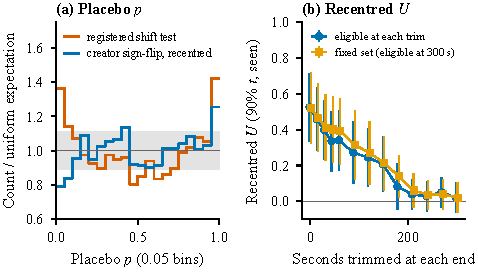
\includegraphics[width=\columnwidth]{floats/fig_hthree.pdf}
\caption{H3's calibration and trim. (a) Placebo: sets per $p$ bin over the count expected under a uniform $p$, with a
binomial 90\% band (CAL, sets of \HThreeCreators{} seen creators); the registered circular-shift $p$ piles up in both
tails because it holds creators fixed, while a creator sign-flip on the recentred $U$ stays near nominal. (b) Trim:
recentred $U$ (creator-equal mean, 90\% $t$ interval) against the seconds trimmed from each end, seen creators only.
Exploratory.}
\label{fig:hthree}
\end{figure}

\begin{figure}[t]
\centering
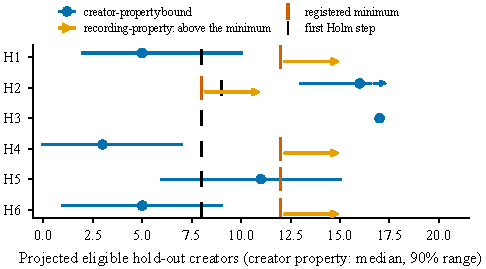
\includegraphics[width=\columnwidth]{floats/fig_eligibility.pdf}
\caption{Projected eligible hold-out creators per hypothesis, under CAL's two bounds: eligibility as a property of the
creator (filled dot, the bound the announcement of 02:50 rests on; median and 90\% range, a dashed arrow where the upper
end is not drawn) and of each recording (arrow from the minimum: its median lies above the minimum; neither its median
nor its range is drawn, as the projections are capped at a count this paper withholds). Solid tick, the registered ``not run'' minimum; black tick, the smallest count at which an exact sign-flip can
pass 0.005 (\MinCreatorsOneSided{} one-sided, \MinCreatorsTwoSided{} two-sided). H3 shows its realised count; H5 is one upper bound
from pilot titles. Projections from model-coded pilot labels, not counts.}
\label{fig:eligibility}
\end{figure}

\begin{figure*}[tp]
\centering
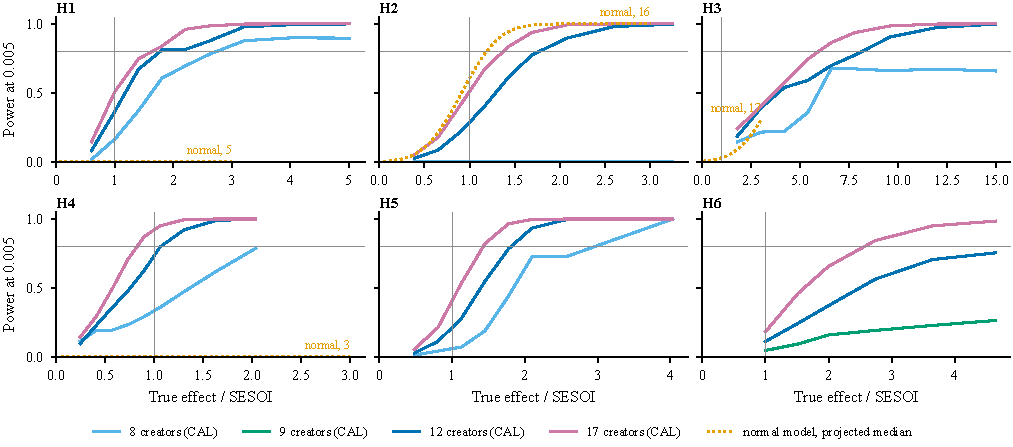
\includegraphics[width=\textwidth]{floats/fig_power.pdf}
\caption{Power of a creator sign-flip at the first Holm step (0.005) against the true effect in units of the smallest
effect of interest: CAL's seen-creator analogues (H1 to H5) and CAL's planted simulation for H6, at the creator counts
named in the legend, and, dotted, a normal model at the projected median for H1 to H4 only. Analogues carry no labels
and are not hypothesis quantities.}
\label{fig:power}
\end{figure*}

\begin{figure}[t]
\centering
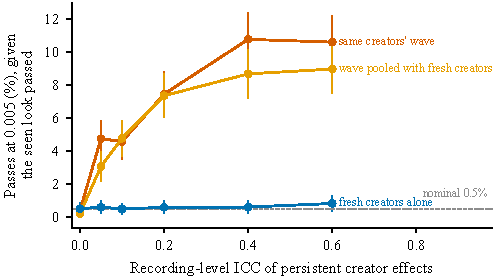
\includegraphics[width=\columnwidth]{floats/fig_plasmode.pdf}
\caption{Why a wave of the same creators cannot replicate. Plasmode under a population null with persistent creator
effects (seen cluster sizes and within-creator pace residuals): share of cases in which a one-sided test at 0.005 passes,
given that an exploratory seen look passed at 0.05. A wave of the same creators passes in
\PlasmodeWaveLo--\PlasmodeWaveHi\% of cases across the simulated recording-level ICCs; fresh creators alone pass at about
nominal. Bars: 90\% Monte Carlo intervals.}
\label{fig:plasmode}
\end{figure}

\paragraph{Deviations and contacts.} Table~\ref{tab:deviations} and Figure~\ref{fig:timeline} carry
Section~\ref{sec:deviations}; Table~\ref{tab:contacts} lists every hold-out contact named in Section~\ref{sec:limits}.
The \NCloudOnlyObjects{} cloud-only metadata objects are to be read once, after freeze 2, in one logged read-only pass
(registry 03:08; moved here from Section 9 by the page limit, results round); the registry records no such read yet.

% INTEGRATOR (2026-11-21): the deviation table is about three pages tall; the builder writes it in three parts of
% consecutive, numbered rows. The class column uses the seven classes of Section 8.
\begin{table*}[tp]
\centering
\small
% tab_deviations.tex: GENERATED by the private builder build_numbers.py at 2026-11-26T03:59:48Z; label tab:deviations. The writer adds the float,
% the caption and the label. Sources: a private file of the run (named in the private build record); REG/registry.md
% Part 1 of 6. Rows: D6 (to 00:50 UTC), the registry's deviation table (A10 Part 8, rows from 01:10 UTC), and registry rows written after it was last brought up to date.
{\tiny\setlength{\tabcolsep}{2pt}
\begin{tabular}{@{}rp{0.065\textwidth}p{0.1\textwidth}p{0.42\textwidth}p{0.09\textwidth}p{0.16\textwidth}l@{}}
\toprule
 & UTC & Applies to & As done (against the registry of 20 Nov, 19:47 UTC) & Known then & Direction & Class \\
\midrule
1 & found 2026-11-20 about 23:00 (panel round 2) & H3 reference distribution & shift reference ignores variation between creators; creator-level placebo rejects 1.3-1.6\% at nominal 0.5\% (CAL) & H3 hold-out and seen results & looser than R1 as registered & looser \\
2 & found after the test & H3 estimand centring & U has mean -0.063 under its own reference; recentred seen value 0.083 (F5) & yes & neutral (bias, not a choice) & neutral \\
3 & 20:38 (freeze) without the audit & H3 interval against CA & percentile creator-then-recording bootstrap; CA had not run before the hold-out was spent (F11) & no & looser & looser \\
4 & 20:38 & CA-1 coverage audit and planted-effect check & skipped for H3 & no & looser & looser \\
5 & 20:39 & Leave-one-creator-out range & not reported for H3 & no & looser & looser \\
6 & 2026-11-20 20:49 & H3 verdict and A6 & 'supported' reported, then H3 dropped by the owner (A6, 20:49 UTC) after reading the result & yes (H3 hold-out and seen results) & neutral (claim withdrawn, row kept) & neutral \\
7 & 2026-11-20 20:49 & H3 registered wave replication & closed by A6: not tested again as confirmatory & yes & neutral & neutral \\
8 & 2026-11-20 20:39-20:49 & A5 stricter verdict & 'supported' also needs the 90\% interval over creators to exclude 0, for hypotheses not yet run & yes (H3) & stricter & stricter \\
9 & 2026-11-20 19:47 (with the freeze) & A2 'uninformative' pruning & no operational definition of 'uninformative' written & no & looser (undefined) & looser \\
10 & 2026-11-20 about 22:45 & A8 no human check & no person checks any label; strongest verdict 'supported (model-coded)' & yes (H3, bridge, pilots) & looser & looser \\
11 & 2026-11-20 about 22:45 & A9 H8 dropped; stricter amendments in principle & H8 dropped, counted as run with p = 1; sign-flip p, fixed Holm count of 10, 'not determinable' outcome approved in principle & yes & H8: neutral; amendments: stricter & neutral \\
12 & 11-21 16:07 & A10 exact text of the stricter amendments & A10 and its companion parts 2 to 7 entered in the registry from A10-draft.md (its hash cited there), before freeze 2 and any hold-out label & SP, SP-C; no hold-out label & stricter & stricter \\
13 & 2026-11-20 about 22:50 & A11 verification by language models & a third, larger model and known-answer texts stand in for the human check & yes & looser than R7; neutral against A8 & looser \\
14 & 2026-11-20 about 23:10, after the H3 test & Selection rule of the cohort & 'channelling mediums' stated by the owner & yes & neutral (descriptive, post hoc) & neutral \\
15 & 2026-11-20 about 22:45 & Holm count & count fixed at 10, unrun at p = 1 (A9 in principle) & yes & stricter & stricter \\
16 & pending at 00:50; settled 11-21 16:06 & H7 and H9 smallest effects & H7 margin 0.01 shown to be unreachable; block-reference units proposed (F9); settled at 16:06 (row 87): H9 keeps the placeholder 0.2 standardised units (a mixed deviation), H7 is not run & seen creators only & to be set; must not be looser; settled 16:06 & other \\
17 & 2026-11-20 22:30 and 23:10 & Budget & 120 USD (caps 60/50/4, 115 total), then a warning with a 250 USD loop guard & yes & neutral for inference & neutral \\
18 & 2026-11-20 13:00 to 23:07 & Hold-out definition and contacts & four contacts before freeze 2 (snapshot tables, run report heat map at 20:09, H3 run, panel metadata load) plus the planned TABLE extraction; the contact table lists every contact, those of 21 November included (public-output generators, the one-off seen-derivative script) & partly & looser than the stated rule & looser \\
19 & 2026-11-21 about 00:30 & Freeze-1 instruments & checkability (time window 0.55, place not published (fewer than 5 creators)) and titles (not published: fewer than 5 creators) failed; middle model made the record with larger-model adjudication & pilot results on seen and check creators & looser (gate failed, instrument kept) & looser \\
20 & 11-21 commit 22:56:59 & - & Hold-out contact log added & PAN & disclosure & other \\
21 & 11-21 commit 23:03:43 & H1, H4, H6 & Primary definitions: broad own voice; an offer alone does not end a claimed voice & CAL, G (voice pilots) & neutral; chosen before any label of the frozen instrument & neutral \\
22 & 11-21 01:10 & reliability, wording, exploratory & V4 and V6 merged for reliability reporting; "guided steps" wording; the adjudicating model fixed; the other-vendor reader added; timeline built after the seen forecast labels & G (verification pilot) & neutral; the other-vendor reader is stricter & neutral \\
23 & 11-21 01:15 & H1, H4, H6 & Voice: variant B, with the one revision spent on gate C (0.834 against 0.90); if gate C fails again, H1, H4 and H6 are not run & G & stricter (consequence fixed beforehand) & stricter \\
24 & 11-21 01:15 & H6 & Ask check input states the number of candidates; ask gate rerun & G & neutral & neutral \\
25 & 11-21 01:15 & H1, H4, H6 & Middle model is the voice record on the hold-out; H4's yardstick comes from small-model labels on all seen recordings & G & neutral & neutral \\
26 & 11-21 01:15 & all labelled & Gate rule: combined rule; an instrument below its floor means "not run", p = 1 & G & stricter (A10.5) & stricter \\
27 & 11-21 01:15 & H2, H5 & Forecast protocol defaults: H5's share and minimum hits as CAL drafted them; H2 also on one-voice recordings; calendar class; titles without a cue coded as not presented; seen creators labelled first & CAL & H5's minimum guarded (A10.4); the rest neutral & guarded \\
28 & 11-21 01:20 & H6 & Ask check: context units are for reading only; a class listed twice is accepted & G & neutral & neutral \\
\bottomrule
\end{tabular}}

\caption{Deviations from the registry frozen \RegistryFrozenStamp{} (hypotheses SHA-256 prefix
\HypothesesShaPrefix), part 1 of 6: row number; UTC of the change; what it applies to; what was done against the
registry; results known at the time; direction as recorded; and its class (stricter; guarded by amendment A10; neutral;
looser; mixed: stricter for some uses and looser for others, or of a direction not known in advance, outside the guard;
exploratory; budget or operations; other: disclosure, correction of the record, the freeze-1 entry, reporting (the
public results file and its republications), or not yet decided).
\NDeviationRows{} rows: the paper review's table, the registry's deviation table (A10 Part 8, entered at \ATenStamp;
its rows of contacts, of the freeze-1 entry and of corrections of the record included), and the registry rows written
after that table was last brought up to date (16:06 to 23:34); no deviation is listed twice. The relayed-voice merge of
02:55 is classed looser here, against A10's own record, and applies to H1 and H6 (registry 04:55 (a)), where A10 lists
H1 and H4 (Section~\ref{sec:instruments}).}
\label{tab:deviations}
\end{table*}

\begin{table*}[tp]
\centering
\small
% tab_deviations_b.tex: GENERATED by WORK/build_numbers.py at 2026-11-22T00:15:32Z; label tab:deviations. The writer adds the float,
% the caption and the label. Sources: REV/build-descriptive/out/D6/D6-deviation-table.csv; REG/registry.md
% Part 2 of 6. Rows: D6 (to 00:50 UTC), the registry's deviation table (A10 Part 8, rows from 01:10 UTC), and registry rows written after it was last brought up to date.
{\tiny\setlength{\tabcolsep}{2pt}
\begin{tabular}{@{}rp{0.065\textwidth}p{0.1\textwidth}p{0.42\textwidth}p{0.09\textwidth}p{0.16\textwidth}l@{}}
\toprule
 & UTC & Applies to & As done (against the registry of 20 Nov, 19:47 UTC) & Known then & Direction & Class \\
\midrule
29 & 11-21 01:30 & H6 & Ask gate C failed (0.721), so the one revision is used: the union of two draws. The gate row is not switched to the row that passed. A second failure means H6 is not run (declared before the rerun). Output cap set & G & stricter or neutral & stricter \\
30 & 11-21 02:00 & - & Budget 130 USD with a hard stop; batch interface; restart in the guarded environment, with no label, gate or estimate changed & - & budget, operations & budget \\
31 & 11-21 02:20 & H6 & Ask rerun: gate C passes; gate B fails for the small check, so the middle model becomes the ask-check record & G & neutral (both measured on the same runs) & neutral \\
32 & 11-21 02:25 (note 3) & -; H6 rows & Discovery stopped by a hard cap; the H6 census keeps the middle-model find; a hold-out preparer for the rewording rows & - & budget; stricter (rows) & budget \\
33 & 11-21 02:40 & instruments & Known-answer battery cap raised for the six items that check frozen instruments & G & budget & budget \\
34 & 11-21 02:45 & all labelled & Listing repair (25 seen transcripts had no listing row); format of the freeze-2 record & - & neutral (data repair) & neutral \\
35 & 11-21 02:50 (note 4) & HR & Hold-out robustness rows released on `verification\_passed` and `verification\_basis`, not `human\_passed` & - & neutral (follows A8) & neutral \\
36 & 11-21 02:50 (note 4) & paper & The paper becomes a measurement-and-protocol paper; first-round results are reported as model-coded descriptions & REV & stricter (claims) & stricter \\
37 & 11-21 02:50 (note 4) & H1, H4, H6 & A8 stands; H1, H4 and H6 announced as probably not determinable (median 5, 3 and 5 eligible creators against 12) & REV, CAL & stricter (announced in advance) & stricter \\
38 & 11-21 02:50 (note 4) & measurement & Anchor against text made or edited by people: word error rate against text made or edited by people, on seen creators; grid-shift re-decode & REV, BR & exploratory & exploratory \\
39 & 11-21 02:50 (note 4) & public outputs & Public outputs: rows and bins with fewer than 5 creators merged; dashboard statements corrected & REV & disclosure & other \\
40 & 11-21 02:50 (note 4) & all & Registry additions before freeze 2: A10; hold-out-only primary; "uninformative" defined; exploratory reporting plan & REV, CAL & A10 guarded; "uninformative" stricter for the claims; hold-out-only primary has less power and, with the rule of 04:55 (h), cannot make a verdict easier to reach (Part 4) & guarded \\
41 & 11-21 02:50 (note 4) & H2, H5 & H2 and H5 revised at the analysis level (M9). H2: flagged statements, and reduced to its parts with at least 5\% prevalence. H5: excludes units next to a self-naming cue; three Q2 assignments. Second readings by another model & REV, G & changes registered estimands before any label; direction not known in advance; the rows without each change are reported beside (Part 7) & mixed \\
42 & 11-21 02:50 (note 4) & H3 & H3: the wave replication reported as not run; one logged rerun of the frozen H3 code on the hold-out after freeze 2 (exploratory) & REV, CAL & exploratory & exploratory \\
43 & 11-21 02:50 (note 4) & exploratory & Prediction timeline: methodological agnosticism; source types reported as separate rows & REV & exploratory; stricter wording & exploratory \\
44 & 11-21 02:50 (note 4) & - & Left to the owner: ethics, lawful basis, inclusion rule, external registration, unlinking the site & REV & not decided & other \\
45 & 11-21 02:53 & H2 (forecast class) & Forecast critic: one boundary sentence; forecast gates rerun; the known-answer relayed arm rescored & G (known-answer battery) & neutral (follows the codebook); before freeze 1 & neutral \\
46 & 11-21 02:53 & H1, H4, H6 & Voice: the middle model stays the hold-out record; seen voice descriptives come from the middle-model subset & G & neutral & neutral \\
47 & 11-21 02:55 & H1, H6 (H4: secondary row only; registry 04:55 (a)); A10 lists H1, H4 & Voice revision 3: relayed voice merged into claimed voice (Part 5) & G & looser (post-hoc merge decided after the gate result; by the letter of plan 3.4, not run; A10 records it as: stricter (consequence fixed in plan 3.4)) & looser \\
48 & 11-21 02:55 & H1, H4, H6 & Voice settings for freeze 1; the middle model at effort low, a recorded deviation from the plan's effort rule & G & neutral & neutral \\
49 & 11-21 commit 02:56:03 & record & Stamps of nine rows corrected from 03:00 to 02:50 & - & correction of the record & other \\
50 & 11-21 03:08 & all & Order of spending under the 130 USD stop & - & budget & budget \\
51 & 11-21 03:08 & freeze 1, HR, H1, H4, H6 & Replacement of the human check in every rule that names it (Part 2) & G, REV & follows A8; no floor lowered & neutral \\
52 & 11-21 03:08 & H1, H2, H4-H7, H9, H10 & A10 with its guard (Part 1) & CAL, REV & stricter or guarded & stricter \\
53 & 11-21 03:08 & all labelled tests & Recognizer rule (Part 6) & PAN & stricter & stricter \\
54 & 11-21 03:08 & exploratory; H3 wording & Panel decisions adopted: H3 wording; topic reading A, decided at about 02:30 UTC after its stage-1 results; and others & PAN, CAL & exploratory; one reading chosen after its results, stated openly & exploratory \\
55 & 11-21 03:12 & H2 (forecast class); timeline & Forecast critic: the relayed-forecast sentence counted as its one revision; gate D passes on its lower bound; the ten-class label fails stability (0.77 against 0.85) and is a description only; the known answer is not changed & G (gates, known-answer battery) & neutral for the registered uses, which need F1 against the rest (gate D's contrast) & neutral \\
\bottomrule
\end{tabular}}

\caption{Deviations from the registry, part 2 of 6 (columns as in part 1).}
\label{tab:deviations-b}
\end{table*}

\begin{table*}[tp]
\centering
\small
% tab_deviations_c.tex: GENERATED by WORK/build_numbers.py at 2026-11-22T01:51:42Z; label tab:deviations. The writer adds the float,
% the caption and the label. Sources: REV/build-descriptive/out/D6/D6-deviation-table.csv; REG/registry.md
% Part 3 of 6. Rows: D6 (to 00:50 UTC), the registry's deviation table (A10 Part 8, rows from 01:10 UTC), and registry rows written after it was last brought up to date.
{\tiny\setlength{\tabcolsep}{2pt}
\begin{tabular}{@{}rp{0.065\textwidth}p{0.1\textwidth}p{0.42\textwidth}p{0.09\textwidth}p{0.16\textwidth}l@{}}
\toprule
 & UTC & Applies to & As done (against the registry of 20 Nov, 19:47 UTC) & Known then & Direction & Class \\
\midrule
56 & 11-21 03:12 & H2 (forecast class); timeline & Class of record for every registered and timeline use: F1 against the rest, whose stability passes gate C (0.93). Gate C in the annotation plan reads "at least 85\% of units keep their class", the ten-class label; the coarser class was chosen at 03:12, after the ten-class row had failed & G (the failed ten-class row) & deviation from gate C's wording, chosen after its result and stated openly: looser for the gate (a two-class label keeps its value more easily than a ten-class one); neutral for the registered uses, which read only F1 against the rest & looser \\
57 & 11-21 03:12 & H2 (checkability) & Production adjudication of checkability keeps the large model fixed at 01:10; the recorded gate figures, made with another tier, stay as recorded and the difference is reported & G & neutral (decided before these figures) & neutral \\
58 & 11-21 03:18 & exploratory & Entrance experiment: pattern version 1 is primary, version 2 (revised after the check reading) a labelled secondary row; the names lexicon pinned to the store version of its seen run; counts as cue counts and upper bounds & G (check reading), PAN & exploratory; version 2 made after a reading, labelled & exploratory \\
59 & 11-21 03:21 & H1, H4, H6; HR & Other-vendor voice check (gate VG-6) fixed before its sealed figures are opened: comparator the stored OpenAI majority; on failure H1, H4 and H6 are flagged and capped at "not determined" and the HR (b, c) money returns; on a pass it serves the HR (b, c) release rule, overriding the programme's rule that the fallback cannot pass & G (figures sealed) & stricter for H1, H4 and H6; looser for the HR release (the fallback can pass), fixed before the figures & mixed \\
60 & 11-21 03:21 & instruments (H2, H5) & Verification before freeze 1: typed guided fields and shard sizes kept; the sentence-code instrument stays at one unit per call, the gated form, against the protocol text's 15 per call; the time instrument's role stability reported as a limit & G & neutral; a deviation from the protocol text, the gated form kept & neutral \\
61 & 11-21 04:55 & - & Budget guard at worst case: the 130 USD hard stop and every tag cap are tested with every open batch job at its worst case plus the new step's worst case; the protocol's one repeat reserves its full output cap; batch reservations hold twice the measured mean output (at most the cap), measured on seen pilot and gate stores; production waves under 128 USD at worst case; the verification shard's pins amended for four files after its requests were rebuilt and found unchanged & FRV & budget, operations; the hard stop holds at worst case again & budget \\
62 & 11-21 04:55 & H1, H2, H4-H7, H9, H10 & Decisions on the freeze-readiness open points: (a) H4's primary stays the embodied voice (V2) as registered, V2 + V3 a secondary row without a verdict (Part 5); (b) the model-stratified recognizer row built as written (Part 6); (c) H5's HKSJ random-effects row (A10.7); (d) each registered version under the guard uses the interval hypotheses.md registers for it (guard); (e) "a possibility" leaves H2's shared-wording flag (Part 7); (f) label files opened only after the permission check (Part 4); (g) "not determinable" when either guarded version is (guard); (h) no replication wave, the hold-out the only confirmation sample (Part 4); (i) H7's verdict against both margins (A10.6); (j) the wider Mantel-Haenszel interval until the coverage repeat (A10.4); (k) H6's registered version uncentred, its null mean reported (A10.7); (l) A10.k = CAL A(7 + k) in text and code; (m) H10 not run in the first round, its readers replaced before it is run (Part 2); (n) the simulation battery on the earlier code stopped, a new one on the final code & FRV, DBL, CAL & (a), (d) and (k) follow the registered text; (b) and (c) add rows; (g), (h), (i) and (j) stricter; (e) changes H2's primary sample, direction not known in advance, and removes a selection on the outcome; (f), (l), (m) and (n) neutral or operations & stricter \\
63 & 11-21 04:55 & H2, H5 & Second reading (02:50) recorded on seen check creators; the checkability codebook is not changed before freeze 1; H2 gets a sensitivity row in which a time window taken only from the period of the talk counts as NO; the reading covers checkability and the sentence codes, not commitment & DBL & stricter (one more row); the primary already does not count such a time window read as YES, so the row differs from it only where it is read "cannot tell" (Part 7) & stricter \\
64 & 11-21 freeze-1 entry: 04:58:22 & instruments & Freeze 1 of the instruments: record, configuration, models, code and 83 prompt and schema files fixed by hash; seen production unlocked, hold-out and other labels only after freeze 2 & G, FRV, DBL & procedure freeze & other \\
65 & 11-21 04:59 (note 5) & freeze 1; HR & Freeze 1 does not wait for the known-answer battery's last voice batches (pending since about 02:47 UTC), against the rule of 03:08 that freeze 1 waits on the battery's pre-set rules (Part 2); the request-id fixture retaken for the four forecast-critic lists only & G (the battery's finished items) & deviation from the 03:08 rule, stated with its reason: looser for freeze 1's timing; no instrument is affected (each has spent its revision), and the battery still serves the paper and the HR (b, c) release & looser \\
66 & 11-21 04:59 & H1, H4, H6; HR & Gate VG-6 opened after freeze 1 with its seal verified: kappa 0.91 (0.84 to 0.95) on claimed, own and other voice, 0.91 (0.83 to 0.96) on the embodied contrast; it passes, so no vendor flag applies to H1, H4 and H6, and VG-6 meets its part of the HR (b, c) release & VG & neutral (a result read under the meaning fixed at 03:21) & neutral \\
67 & 11-21 05:00 & seen labels & Seen-creator production starts through the batch interface under freeze 1, one driver per instrument, with its cost projection (about 20 USD) reported before sending and spending stops on three of its lines & G & budget, operations & budget \\
68 & 11-21 06:33 & seen labels; known-answer battery & The heads of the seen voice and forecast chains move to the standard interface after their batch jobs had returned nothing for 80 to 85 minutes (open jobs cancelled first; request ids and bodies unchanged; about 2 USD extra); three known-answer batch jobs re-sent after cancellation at 05:44 & - & budget, operations & budget \\
69 & 11-21 06:36 & exploratory outputs & Exploratory reporting plan and its addendum 1 registered by hash. Lead's decisions in the addendum: the public rows of the word-error-rate anchor keep machine texts of different origin apart and withhold the pooled automatic row, a departure from the plan's section 3; the diagnostic cards' verdicts are not reported; the missing measures of the grid-shift re-decode (BR-GS) are built from the existing re-decodes; the abstract gives the caption figure as agreement only; the anchor's hold-out part runs after freeze 2 as a logged contact & BR-b & exploratory; hashed after the anchor's first tables, which the addendum names; the departure is stated with its reason & exploratory \\
\bottomrule
\end{tabular}}

\caption{Deviations from the registry, part 3 of 6 (columns as in part 1).}
\label{tab:deviations-c}
\end{table*}

\begin{table*}[tp]
\centering
\small
% tab_deviations_d.tex: GENERATED by WORK/build_numbers.py at 2026-11-22T01:51:42Z; label tab:deviations. The writer adds the float,
% the caption and the label. Sources: REV/build-descriptive/out/D6/D6-deviation-table.csv; REG/registry.md
% Part 4 of 6. Rows: D6 (to 00:50 UTC), the registry's deviation table (A10 Part 8, rows from 01:10 UTC), and registry rows written after it was last brought up to date.
{\tiny\setlength{\tabcolsep}{2pt}
\begin{tabular}{@{}rp{0.065\textwidth}p{0.1\textwidth}p{0.42\textwidth}p{0.09\textwidth}p{0.16\textwidth}l@{}}
\toprule
 & UTC & Applies to & As done (against the registry of 20 Nov, 19:47 UTC) & Known then & Direction & Class \\
\midrule
70 & 11-21 06:39 & seen labels & Every small-model stage of the seen chain (sentence codes, asks find and small-model check) moves to the standard interface after its batch jobs were cancelled and collected; the middle-model and title stages stay in batch; extra cost of all moves about 5 USD; the committed spend projected after the seen and hold-out chains stays under the 120 USD warning only if the hold-out small-model stages go through batch or the queue clears & - & budget, operations & budget \\
71 & 11-21 contact log: about 03:00 to 06:35 & public outputs & Hold-out contact: the public-output generators loaded the run report's per-recording timing cache, hold-out and other creators included, to rebuild distribution tables; no word, label or hypothesis statistic was read or produced & - & disclosure; one generator no longer loads the cache and the other two are changed to read seen creators only for positional measures (closed by the entry of 06:49:10) & other \\
72 & 11-21 06:44 & H2, H5, H6, H9; freeze 2; paper & Decisions on the second verification of the hypothesis code, before freeze 2 and any hold-out label: (1) a seen-only permission path: before freeze 2 the analysis code may open labels/seen only, refusing any other path and any record whose group is not seen, for the freeze-2 constants, CAL part (f) and the A10.7 null-mean check; the path is part of the code freeze 2 hashes (Part 4; A10.7); (2) one freeze-2 record, `llm/freeze2.json` with the six keys of 02:45, which the analysis code checks against its modules (Part 4); (3) H6's amended OE and Mantel-Haenszel rate ratio centred per recording, the registered version as registered (A10.4; guard); (4) H9's creator-bootstrap interval drawn creators, then recordings (R1) in both versions, with fewer draws allowed in the simulation battery if stated (A10.7; guard); (5) A5 for H5 and H6 on both the t interval of the creator OE values and the wider Mantel-Haenszel interval (A10.1; A10.4); (6) H6's $\delta$ for "uninformative" stays log 2 (Part 3); (7) the M9 revisions stay outside the guard, the rows without them reported with their own verdicts (Part 7); (8) H2's FRAME row stays as built (Part 7); (9) creator-by-model strata for H5 in the model-stratified row (Part 6); (10) times cited in the paper are commit times (this table); (11) the full simulation battery started at 04:57 on earlier code was stopped at 06:42, a new one is to run on the final code & SV, FRV & (1) neutral for every verdict: a narrow exception to (f) that opens only seen labels, which freeze 1 released for production, and computes no hypothesis quantity; (2) neutral, fails closed; (3) guarded: it changes the amended statistic and removes a centring fault in H6's predicted direction; (4) and (6) follow the registered text (for (6), the stricter $\delta$ of log 1.5 was not taken); (5) stricter; (7) and (8) neutral, confirming Part 7; (9) a sensitivity row only, now exactly within one model; (10) record; (11) operations & neutral \\
73 & 11-21 contact log: 06:49:10 (note 6) & public outputs & Hold-out contact: a one-off script loaded the run report's per-recording timing cache once and kept only the rows of the 71 seen creators (by the creator sets of freeze 1), writing a seen-only derivative; nothing was computed on any other row, and the script refuses to run again. Since then no generator reads the cache: whole-run counts come from ledger fields, every timing measure from the seen derivative & - & disclosure; closes the generators' use of hold-out timing rows & other \\
74 & 11-21 07:50 (note 7) & seen labels & The forecast critic (about 42,600 small-model requests) was first sent through batch to save about 2.2 USD, under a rule fixed beforehand: cancel if under half is back after 30 minutes. None of the first 3,000 came back in 30 minutes, so its batch jobs were cancelled and collected and it runs through the standard interface (estimate 4.4 USD, run limit 6 USD). Seen titles, voice and asks are done & - & budget, operations; the rule fixed beforehand was applied & budget \\
75 & 11-21 commit 08:24:06 (note 7) & record & The row of 07:50 moved from the hold-out contact log into the table of decisions (commit message: "insertion slip"); its text unchanged & - & correction of the record & other \\
76 & 11-21 08:33 & known-answer battery; HR & Known-answer battery: its voice parts (the revision-3 arms and the voice audit), waiting in the small model's batch queue since about 02:47 (cancelled and re-sent once at 05:44), finish through the standard interface after both lanes' open batch jobs were cancelled and collected; a few hundred requests, about 1 USD, inside the battery's tag cap tested at worst case & - & budget, operations & budget \\
77 & 11-21 09:10 & HR; paper & Known-answer battery complete (constructed texts; exploratory, an upper bound and not accuracy on the corpus): with voice revision 3 the small model's recovery rose on the relayed-voice, own-offer and interview arms, and the canary gates pass for voice, asks and forecasts. With VG-6 (04:59), the row states both parts of the HR (b, c) release rule met; HR (b, c), a tier-5 line, starts only within the 120 USD rule of 03:08 & G (the battery's results) & neutral: a result read under rules fixed before it (03:08, 03:21); no instrument changes & neutral \\
78 & 11-21 09:19 (note 8) & H5, H6; freeze 2 & Decisions on the third verification of the hypothesis code, before freeze 2 and any hold-out label: (1) H6's amended version keeps OE centred per recording, but its reference becomes a conditional Monte Carlo draw under the per-recording null (each recording's asks from a binomial with its claimed share, given its ask count) in place of the sign-flip, because exact enumeration showed the one-sided sign-flip rejecting 1.93\% at 0.005 with one ask a creator at a claimed share of 0.3; the battery gains a null scenario with shares below one half and 1 to 3 asks a creator (A10.4); (2) the A10.7 null-mean tolerance of the OE versions is a tenth of the smallest effect on the OE scale, not 0.1 on the share scale (A10.7); (3) the null check keeps recordings without an ask file, as the analysis does (A10.7); (4) a verifier's test file that globbed the production label tree leaves the code's package; (5) the hypothesis code is committed to the analysis branch before freeze 2, and A10 keeps its `**A10.` heading for the labelling side's check (Part 4); (6) H5's stratified-row choice for a stratum without hits on one side stays as written (weight at most 0.25), stated as a limit & V3 & (1) guarded (the amended version only); the row said it "can only make a verdict harder to reach", which the row of 11:08 corrects; replaced at 11:08 (1); (2) stricter (a tighter check); (3) neutral: the check reads the creators the analysis reads; (4) neutral: protects the hold-out; (5) record; (6) a sensitivity row, a stated limit & guarded \\
79 & 11-21 11:08 & H6 & Correction to the row of 09:19: the conditional reference does not "only make a verdict harder to reach"; on some data its p is below the sign-flip's & V4 & correction of the record & other \\
\bottomrule
\end{tabular}}

\caption{Deviations from the registry, part 4 of 6 (columns as in part 1).}
\label{tab:deviations-d}
\end{table*}

\begin{table*}[tp]
\centering
\small
% tab_deviations_e.tex: GENERATED by WORK/build_numbers.py at 2026-11-22T01:51:42Z; label tab:deviations. The writer adds the float,
% the caption and the label. Sources: REV/build-descriptive/out/D6/D6-deviation-table.csv; REG/registry.md
% Part 5 of 6. Rows: D6 (to 00:50 UTC), the registry's deviation table (A10 Part 8, rows from 01:10 UTC), and registry rows written after it was last brought up to date.
{\tiny\setlength{\tabcolsep}{2pt}
\begin{tabular}{@{}rp{0.065\textwidth}p{0.1\textwidth}p{0.42\textwidth}p{0.09\textwidth}p{0.16\textwidth}l@{}}
\toprule
 & UTC & Applies to & As done (against the registry of 20 Nov, 19:47 UTC) & Known then & Direction & Class \\
\midrule
80 & 11-21 11:08 & H6, H9; freeze 2 & Decisions on the fourth verification, before freeze 2 and any hold-out label: (1) H6's amended reference redraws asks by cluster (asks in the same checked unit range or in adjacent units form one cluster; each cluster's voice drawn with the recording's claimed share), and the p that enters the guard is the larger of this cluster-level conditional p and the sign-flip p of OE, so that neither the sparse low-share case (where the sign-flip over-rejects) nor bursts of asks in one voice (where an ask-level reference over-rejects: 7.7\% at 0.005 for bursts of 3) can carry a verdict alone; 99,999 draws in the analysis; a burst scenario in the battery; H6's detectable-effect note from the battery (A10.1; A10.4; guard); (2) H9's content words exclude every variant of the frozen family table as well as the NAMES v2 list forms; (3) contractions whose parts are function words count as function words; (4) masking NAMES v2 forms everywhere (the flat-list form of the released mask) stays, stated as a choice, and the 9 seen transcripts without a stated model enter the model-stratified row as unknown model (Part 6); the seen feature files are written again with (2) and (3) before the freeze-2 constants are computed & V4, FT & (1) stricter than the sign-flip of OE that A10.4 drafted, since the amended p is never below it; against the reference of 09:19 the direction depends on the data; inside the guard; (2) construct, both versions of H9: removes a mechanical raise of same-family content similarity, in H9's predicted direction; (3) construct, both versions of H9, direction not known in advance; (4) a stated choice and a sensitivity row; the re-written feature files: operations & stricter \\
81 & 11-21 11:10 & seen labels; freeze 2 & Seen-creator production complete under freeze 1 (05:01 to 11:10): voice, asks, sentence codes and forecasts for all 1,293 English recordings of the 71 seen creators, titles for the 71 creators; production measured 24.27 USD, committed spend 111.89 USD against the 120 USD warning and the 130 USD hard stop; no hold-out or other-group recording was labelled; the freeze-2 constants are computed from these labels alone & - & budget, operations & budget \\
82 & 11-21 12:52 & H6 & Correction to the row of 11:08: with 99,999 draws the p is reproducible (seeded by its label), but inside about 0.0045 to 0.0055 the side of 0.005 still depends on the draws & V5 & correction of the record & other \\
83 & 11-21 12:52 & H6, H9; freeze 2 & Decisions on the fifth verification, before freeze 2 and any hold-out label: (1) H6's clusters: asks within 5 units of each other (about one minute of speech) form one cluster, chaining; a 10-unit window is a sensitivity row; H6's result states that dependence of asks beyond the window is not modelled; the battery gains a scenario with asks one to three units apart at shares below one half (A10.4; guard); (2) the analysis counts asks of one class whose unit ranges overlap once (the union of two find draws can return one ask twice); the instrument is frozen and unchanged (A10.4; guard); (3) H9's contraction rule also splits ain't and y'all into function words; (4) the analysis refuses a bundle whose feature files mix feature versions (Part 4); (5) the wide mask of 11:08 (2) stays (every token of every family variant, about 6\% of content tokens), which can only lower same-family content similarity; (6) the freeze-2 constants are computed from the seen labels through the seen-only path after these changes, recomputed by a second reader and entered in `constants.py` (Part 4) & V5, FT, SP & (1) corrects a level fault of 11:08's clusters (a burst of 3 asks 2 units apart at s = 0.3, 17 creators: 1.93\% at 0.005 with the clusters of 11:08, 0.23\% with the 5-unit window; A10.4); the amended p stays at least the sign-flip p, so stricter than A10.4's draft; inside the guard; its limit beyond the window is stated; (2) a counting correction in both versions of H6, direction not known in advance; (3) construct, both versions of H9 (20 tokens on the seen transcripts); (4) stricter: fails closed; (5) confirms 11:08 (2); (6) procedure: the constants come from seen labels alone, after every change above (14:00 UTC) & stricter \\
84 & 11-21 13:05 & exploratory outputs & Exploratory reporting plan, addendum 2 registered by hash (`c35f316b...`): it corrects addendum 1 (normaliser version 2 made at 03:31:13 to 03:31:26 UTC; the edit of 03:43 changed only the trimming rule), records version 1 as rebuilt exactly and run (rates not printed by the pair rule), the public inventory form, the precision check without a band, the choices of the grid-shift re-decode made while building, the per-cell interval seeds, the merged rows, and the dominance and pair rules applied to every public cell of the anchor and the re-decode; and it fixes the hold-out anchor's reading of caption makers before freeze 2 & BR-b & exploratory; corrects the record of addendum 1 (row of 06:36); every choice made after a result is named & exploratory \\
85 & 11-21 15:14 & H1, H4, H5, H9; freeze 1; freeze 2 & Before freeze 2. (1) Freeze 1, amendment 1: the hold-out and other-group feature files that H1, H4, H5 and H9 read had no guarded path (hold-out transcripts open only while produce.py is the program, and produce.py had no feature step), as the analysis code's README foresaw. produce.py gains a command `features GROUP` that runs only after freeze 2 for a group other than seen, loads the analysis package's `features.py` only at the SHA-256 that freeze 2 pins for it (so seen and hold-out features come from one source), uses the seen run's names and families inputs (hashes pinned in freeze 2) and writes `labels/GROUP/features` with the same feature version; no instrument, prompt, model, setting or request changes. Freeze 1 is written again for the changed produce.py; the record of 04:58:22 UTC is kept beside it, and seen labels keep their freeze time (Part 4) & SP, DV & operations: a new freeze-1 entry that adds a guarded path for the hold-out features, computed by the code and with the inputs of the seen run; no instrument, label or verdict rule changes & guarded \\
86 & 11-21 15:14 & H4, H5, H6; HR; A10 text & (2) Settled for the A10 text, before freeze 2: the ask merge of 12:52 (2) is a counting correction in both versions of H6, outside the guard (Part 1; A10.4; guard); with CAL part (f) not run, the simulation battery on synthetic creators stands in for planted-effect recovery and the Mantel-Haenszel interval stays the wider of two (A10.4; A10.7 point 3); a recording whose model is in dispute stays out of the model-stratified row (Part 6); H4's yardstick keeps its minimum of 40 own-voice forms per creator, set in code before any seen label existed (0.1474 over 52 creators; 0.156 over 60 without it), stated as a choice (Part 4); H6's registered half-count version stays uncentred under the guard (seen null mean -0.137; A10.7 point 3; guard); the HR (b, c) release also needs CAL's two eligibility conditions, read after the hold-out labels, and its money rule (Part 2); the full battery runs on the frozen code after freeze 2 and fills H6's detectable-effect note (A10.2) & SP, SP-C, V5, DV & the ask merge: a classification of the text, the counting of 12:52 (2) unchanged; the battery for recovery: a weaker check than the seen-label check the draft of A10.7 asked for, read by no verdict; the wider interval: as 04:55 (j), stricter; disputed recordings: a sensitivity row only; H4's yardstick: a stated choice made after both values were known on seen labels, keeping the rule the code held before them; the yardstick scales H4's standardised drops, so it moves the conditions that compare a drop with 0.5 (the kept value is the smaller) and not the sign-flip p, direction not fixed; H6's registered version: follows the registered text (04:55 (k)); the HR (b, c) release: follows the rule of 03:08 and A10.2, stricter than the row of 09:10 read alone; the battery after freeze 2: operations, and H6's detectable-effect note is filled after freeze 2 rather than before it as A10.2 asks of the others & stricter \\
\bottomrule
\end{tabular}}

\caption{Deviations from the registry, part 5 of 6 (columns as in part 1).}
\label{tab:deviations-e}
\end{table*}

\begin{table*}[tp]
\centering
\small
% tab_deviations_f.tex: GENERATED by WORK/build_numbers.py at 2026-11-22T00:15:32Z; label tab:deviations. The writer adds the float,
% the caption and the label. Sources: REV/build-descriptive/out/D6/D6-deviation-table.csv; REG/registry.md
% Part 6 of 6. Rows: D6 (to 00:50 UTC), the registry's deviation table (A10 Part 8, rows from 01:10 UTC), and registry rows written after it was last brought up to date.
{\tiny\setlength{\tabcolsep}{2pt}
\begin{tabular}{@{}rp{0.065\textwidth}p{0.1\textwidth}p{0.42\textwidth}p{0.09\textwidth}p{0.16\textwidth}l@{}}
\toprule
 & UTC & Applies to & As done (against the registry of 20 Nov, 19:47 UTC) & Known then & Direction & Class \\
\midrule
87 & 11-21 16:06 & H9; freeze 2 & last points before freeze 2: (1) H9's smallest effect of interest stays at the registry's placeholder, 0.2 standardised units, adopted as the value, since no rule for setting it from seen creators was registered and choosing one with the seen cells computed would let seen data pick the threshold; the seen creators' H9 contrast is a description only; (2) CAL part (f) did not run: every detectable-effect note comes from the full simulation battery on the frozen code, read by no verdict; (3) the hypothesis package normalised to LF line endings, the seen feature files reproduced byte for byte; (4) freeze 1 written again for produce.py with the feature step & SP, SP-C; no hold-out label & mixed (a deviation from the wording 'set from the seen creators', of a direction not known in advance, outside the guard); (2) to (4) neutral or operations & mixed \\
88 & 11-21 16:13 & labels & hold-out production starts under both freezes (16:11), through the standard interface (the small model's batch queue returned nothing to a probe), with run limits and its cost projected before sending; R-hold drawn from ledger fields only & SP-C; no hold-out label & budget, operations & budget \\
89 & 11-21 16:26 & HR; hold-out labels & the hard stop, tested at worst case, refused a standard-interface chunk of the hold-out voice labels (16:20), so the middle model's voice labels went through batch; the money left goes to the registered chain first; HR part (a) and HR (b, c) not bought & hold-out labels in production or done; no test result & budget (HR (a) and HR (b, c), registered robustness rows, not bought) & budget \\
90 & 11-21 16:48 & labels & hold-out production complete under both freezes (16:11 to 16:47), feature files by the frozen feature step; committed spend past the owner's warning of 120 USD, under the hard stop & hold-out labels in production or done; no test result & budget, operations & budget \\
91 & 11-21 17:29 & R-hold; HR & the reliability driver's plan mode refused R-hold (placeholder answers changed the stitched maps and so the request ids); its fix kept as a patch, not applied, so that both freezes stay as written; R-hold runs in run mode with per-command run limits; the HR rewording arms are not run (not released) & hold-out labels in production or done; no test result & budget, operations (no rule of the reliability design changes; only the plan mode's cost preview is lost) & budget \\
92 & 11-21 18:17 & R-hold; HR & R-hold's middle-model arms move from batch to the standard interface after the first batch, its open job cancelled and collected first; HR part (a) not bought, as it would leave less than 1 USD under the hard stop at worst case & hold-out labels in production or done; no test result & budget, operations (HR (a) not bought) & budget \\
93 & 11-21 18:41 & first-round labels; HR & all first-round labelling complete (hold-out, the checkability check on the hold-out, R-hold, the other group); 126.70 USD committed (125.93 measured, the rest held by unreleased reservations of ended runs), past the warning and under the hard stop; no further model call planned for the first round & hold-out labels in production or done; no test result & budget (HR (a) and HR (b, c) not bought) & budget \\
94 & 11-21 19:30 & first-round test inputs; gates & decisions on the first-round test inputs: (1) a driver outside the freeze ran the frozen reliability report body for R-hold, whose frozen command stops in the HR block, and its figures were accepted; (2) voice gate A read per instrument, as the plan states it, a per-stage reading would fail it; (3) the owner's 00:30 exception applied to the title codes as recorded, not extended; (4) the second-model row of H4 reported with the flag 'labels below the reliability floor'; (5) the public results print each failed gate with its figure & R-hold gates; the results for (4) & mixed: (2) and (3) are choices made after a gate result was computed and before the results were read; (1) operations (the frozen code computed every figure); (4) adds a flag after the results and claims nothing & mixed \\
95 & 11-21 20:48 & public results & public results file written: eligible counts stated against their minimums, each failed gate with its figure, figures resting on fewer than 5 creators withheld & first-round results & reporting (no verdict changes) & other \\
96 & 11-21 21:52 & simulation battery & full simulation battery complete on the frozen code, resumed from its checkpoint with fewer workers after a memory stop & first-round results & budget, operations (read by no verdict) & budget \\
97 & 11-21 22:33 & public results & public results file republished at 21:50 (converter fixes; every hold-out checkability part withheld under the engineer's stricter test) and at 22:33 under one rule for every agreement figure, decided by the lead: the positive code comes from 5 or more creators in each reading, and the creators with a statement the readings code differently are 0 or 5 or more; a minor code both readings give alike is not a cell of its own. Under it the hold-out place and quantity parts and the R-hold asks stability figure C are withheld, and three hold-out checkability parts withheld at 21:50 (time window, named actor, observable outcome) are published & first-round results & reporting (no verdict changes; a rule chosen when the figures it would publish were known, for one standard with the guard of the R-hold figures) & other \\
98 & 11-21 23:17 & exploratory outputs (status L, F2) & exploratory round of the reporting plan started under the owner's delegation: the outputs that need no model call, each run, verified and fixed; outputs that need model calls reported as not run; every hold-out run a logged contact & first-round results; no output of this round read & exploratory (code written after freeze 2, a deviation from the plan's 'code frozen in the freeze-2 record', declared before any of these outputs is read) & exploratory \\
99 & 11-21 23:34 & public results & public results file republished at 23:33 after the final pre-push check: the R-hold asks relative-recall figure E withheld under the 22:33 rule (the accepted asks one finder missed come from fewer than 5 creators), as figure C was; counts of valid calls and quotations in the gate texts given as shares without their shortfalls; the file's small-cells statement states the 22:33 rule & first-round results & reporting (no verdict changes) & other \\
\bottomrule
\end{tabular}}

\caption{Deviations from the registry, part 6 of 6 (columns as in part 1).}
\label{tab:deviations-f}
\end{table*}

% INTEGRATOR (2026-11-21): floats/fig_timeline.pdf was re-drawn by the builder with the events after 01:10 UTC; the
% numbers on the marks are keyed in floats/tab_timeline_key.tex, set below the figure.
\begin{figure*}[tp]
\centering
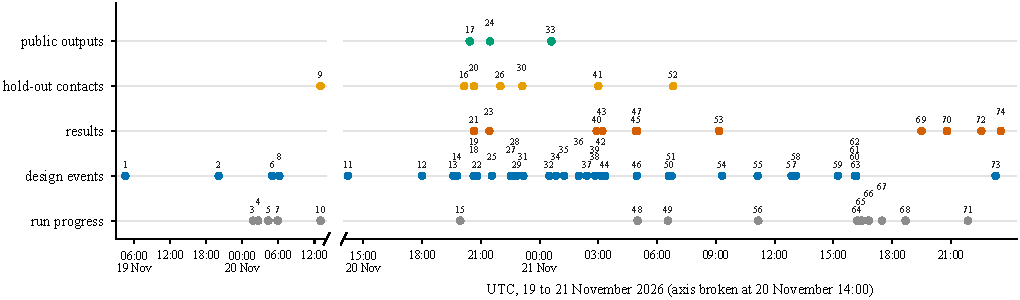
\includegraphics[width=\textwidth]{floats/fig_timeline.pdf}

\medskip
% tab_timeline_key.tex: GENERATED by WORK/build_numbers.py at 2026-11-22T00:15:32Z; label fig:timeline (key). The writer adds the float,
% the caption and the label. Sources: REV/build-descriptive/out/D6/D6-timeline-events.csv; REG/registry.md; LLM/freeze.json
% Key to the numbers of fig_timeline, in two halves side by side.
{\tiny\setlength{\tabcolsep}{2pt}
\begin{tabular}{@{}rllp{0.3\textwidth}rllp{0.3\textwidth}@{}}
\toprule
 & UTC & Lane & Event &  & UTC & Lane & Event \\
\midrule
1 & 19 Nov 04:31 & design & roster table lists 74 channels & 38 & 21 Nov 02:50 & design & paper becomes measurement and protocol \\
2 & 19 Nov 20:03 & design & roster of 101 channels first committed & 39 & 21 Nov 02:50 & design & H1, H4, H6 announced not determinable \\
3 & 20 Nov 01:45 & run & downloads paused (1,946 of 1,976 archived) & 40 & 21 Nov 02:55 & results & voice revision 3 gates \\
4 & 20 Nov 02:38 & run & transcription starts (first progress row) & 41 & 21 Nov 03:00 & contacts & public-output generators load the per-recording timing cache (to about 06:35) \\
5 & 20 Nov 04:19 & run & language fallback phase & 42 & 21 Nov 03:08 & design & content of amendment A10 and its guard written (entered at freeze 2 at the latest) \\
6 & 20 Nov 04:57 & design & owner closes the download goal (30 final failures) & 43 & 21 Nov 03:12 & results & forecast critic revision \\
7 & 20 Nov 05:52 & run & English-first ordering starts (ledger line 251) & 44 & 21 Nov 03:21 & design & VG-6 meaning fixed before opening \\
8 & 20 Nov 06:08 & design & English-first and creator-language rules committed & 45 & 21 Nov 04:55 & results & second reading recorded \\
9 & 20 Nov 13:00 & contacts & first panel tables include 32 hold-out files & 46 & 21 Nov 04:58 & design & freeze 1 \\
10 & 20 Nov 13:00 & run & snapshot of 1,213 finished transcripts (paper numbers) & 47 & 21 Nov 04:59 & results & VG-6 opened: passes \\
11 & 20 Nov 14:13 & design & experiment catalogue (28 experiments) committed & 48 & 21 Nov 05:00 & run & seen production starts \\
12 & 20 Nov 18:00 & design & paper draft committed & 49 & 21 Nov 06:33 & run & seen chains: heads move to the standard interface \\
13 & 20 Nov 19:36 & design & ten candidate hypotheses proposed & 50 & 21 Nov 06:36 & design & reporting plan and addendum 1 registered by hash \\
14 & 20 Nov 19:47 & design & registry frozen (hypotheses.md hash) & 51 & 21 Nov 06:44 & design & hypothesis code: second verification (H6 OE centred per recording) \\
15 & 20 Nov 19:57 & run & run closes: 1,699 of 1,731 recordings transcribed & 52 & 21 Nov 06:49 & contacts & one-off script cuts that cache to the seen creators \\
16 & 20 Nov 20:09 & contacts & run report with position heat map of every creator & 53 & 21 Nov 09:09 & results & known-answer battery complete (voice revision 3) \\
17 & 20 Nov 20:26 & outputs & findings dashboard first published & 54 & 21 Nov 09:19 & design & hypothesis code: third verification (H6 conditional reference) \\
18 & 20 Nov 20:38 & design & H3 procedure frozen & 55 & 21 Nov 11:08 & design & hypothesis code: fourth verification (H6 cluster reference; H9 content words) \\
19 & 20 Nov 20:39 & design & A5 stricter verdict added (after the H3 result) & 56 & 21 Nov 11:09 & run & seen production complete \\
20 & 20 Nov 20:39 & contacts & H3 run opens every English hold-out transcript & 57 & 21 Nov 12:52 & design & hypothesis code: fifth verification (H6 clusters within 5 units; asks counted once) \\
21 & 20 Nov 20:39 & results & H3 result: passes registered rule, interval includes 0 & 58 & 21 Nov 13:05 & design & reporting plan addendum 2 registered by hash \\
22 & 20 Nov 20:49 & design & A6: H3 dropped by the owner & 59 & 21 Nov 15:14 & design & freeze-1 amendment (feature step) decided; A10 text settled \\
23 & 20 Nov 21:26 & results & bridge result: word measures agree, timing differs & 60 & 21 Nov 16:06 & design & H9's smallest effect: the registry's placeholder adopted (a deviation) \\
24 & 20 Nov 21:28 & outputs & dashboard results tab (H3 'supported by the registered rule') & 61 & 21 Nov 16:06 & design & freeze 1 written again (amendment 1, feature step) \\
25 & 20 Nov 21:34 & design & A7: second-round panel gets control and budget & 62 & 21 Nov 16:07 & design & amendment A10 entered \\
26 & 20 Nov 22:00 & contacts & panel coverage script loads \textasciitilde{}415 hold-out metadata files & 63 & 21 Nov 16:10 & design & freeze 2 \\
27 & 20 Nov 22:32 & design & A3 change: budget 120 USD & 64 & 21 Nov 16:13 & run & hold-out production starts (16:11); R-hold drawn \\
28 & 20 Nov 22:45 & design & A8 no human check; A9 H8 dropped & 65 & 21 Nov 16:26 & run & hard stop refuses a standard chunk at worst case (16:20) \\
29 & 20 Nov 22:50 & design & A11 verification by language models & 66 & 21 Nov 16:48 & run & hold-out production complete (16:47) \\
30 & 20 Nov 23:07 & contacts & TABLE whitelisted metadata extraction (planned; done once) & 67 & 21 Nov 17:29 & run & R-hold in run mode (plan mode refused, 16:33) \\
31 & 20 Nov 23:10 & design & selection rule stated; budget becomes a warning & 68 & 21 Nov 18:41 & run & all first-round labelling complete; HR (a), HR (b, c) not bought \\
32 & 21 Nov 00:30 & design & freeze-1 decisions: two instruments failed gates & 69 & 21 Nov 19:30 & results & first-round tests run (18:54 to 19:03); decisions on their inputs \\
33 & 21 Nov 00:36 & outputs & public outputs reduced to distributions & 70 & 21 Nov 20:48 & results & public results file first written \\
34 & 21 Nov 00:50 & design & lead decides under the owner's delegation & 71 & 21 Nov 21:52 & run & full simulation battery complete \\
35 & 21 Nov 01:15 & design & voice: one revision spent & 72 & 21 Nov 22:33 & results & results republished under one rule for agreement figures \\
36 & 21 Nov 02:00 & design & budget 130 USD hard stop & 73 & 21 Nov 23:17 & design & exploratory round of the reporting plan started \\
37 & 21 Nov 02:25 & design & channeler discovery closed & 74 & 21 Nov 23:33 & results & first-round results published (current version) \\
\bottomrule
\end{tabular}}

\caption{Design timeline in UTC, one lane each for run progress, design events, results, hold-out contacts and public
outputs; the key below the plot names each numbered event. Times are commit times or the time stated in the cited
record. A selection of events to the registry's latest row (\TimelineEndStamp): first-round labelling (to
\LabellingDoneStamp), the tests and the decisions on their inputs, the full simulation battery, the first-round results
and their republications (the current version last) and the start of the exploratory round; the contacts of 21
November included; the deviations themselves are in Table~\ref{tab:deviations}.}
\label{fig:timeline}
\end{figure*}

\begin{table*}[tp]
\centering
\small
% tab_contacts.tex: GENERATED by the private builder build_numbers.py at 2026-11-26T03:59:48Z; label tab:contacts. The writer adds the float,
% the caption and the label. Sources: REG/registry.md; REG/hypotheses.md; a private file of the run (named in the private build record)
% Part 1 of 7. Counts of recordings, durations, dates and languages from the run ledger are not contacts. None of these contacts produced a statistic about a registered hypothesis on hold-out text other than H3's registered test (registry).
{\scriptsize\setlength{\tabcolsep}{2pt}
\begin{tabular}{@{}p{0.13\linewidth}p{0.22\linewidth}p{0.44\linewidth}p{0.18\linewidth}@{}}
\toprule
When (UTC) & What touched the hold-out & What was read or written & Status \\
\midrule
20 Nov, about 13:00 (during the run) & The snapshot tables of the first analyst panel (catalogue section 2) & 32 audio files of hold-out creators entered recording-level descriptive tables before the hold-out was declared & Known since the catalogue; stated in the paper's limitations \\
20 Nov, before 19:47 & the first panel's position pilot (H3 disclosure) & drew on 83 creators, more than the 71 seen, so early files of some hold-out creators probably entered it; it produced per-position first-person rates, the reading that suggested H3 & stated in the paper's limitations \\
20 Nov, 20:09 (D6) & The run report and the findings dashboard: speech by position in the recording, recordings by length and share without speech & Timing measures (no words) of every transcribed recording, hold-out creators included, shown in a position heat map and per-creator tables & Found by the second-round panel; stated in the paper's limitations. Fixed 2026-11-21: the run report, the paper figures and the dashboards now draw positional displays from seen creators only, and publish distributions instead of per-creator rows (owner's decision on public identifiers) \\
20 Nov, 20:39 & The registered test of H3, as its frozen procedure allowed & Every English hold-out transcript was opened by the frozen code; the code opened each file more than once across its count-only and full runs & Allowed by the H3 freeze; listed for completeness \\
20 Nov, about 21:50 to 22:15 & A coverage script of the second-round panel (social scientist, round 1) & About 415 metadata files of hold-out recordings were loaded in full (title, description, tags among their fields) and the presence of fields was counted for non-seen creators. The panel reports that no hold-out text was analysed or written out & Breach of the round's rule, found by two other panel members; no hold-out text field is to be extracted before freeze 2 \\
20 Nov, 23:07:10 to 23:07:35 & The TABLE item of the second-round programme & 1,778 local metadata files opened once (hold-out 437, other 57); only time stamps and durations written for non-seen recordings & planned contact, disclosed in advance; done once \\
21 Nov, about 03:00 to 06:35 & The public-output generators of the privacy work (run\_report.py, publish\_progress.py --rebuild, dashboard\_data.py) & They loaded the run report's per-recording cache, which holds timing measures by position (coverage by tenth, quiet stretches, speech seconds) of every transcribed recording, hold-out and other creators included, to rebuild distribution tables with 5 or more creators per cell; no word, label or hypothesis statistic was read or produced & Found by the privacy verifier; dashboard\_data.py no longer loads it; the other two generators are changed to read seen creators only for positional measures \\
21 Nov, at the paper review's build of rv-R3 (before the exploratory reporting plan was written at about 03:00 UTC; exact time not recorded) & Exploratory round, Paper review build (rv-R3): rv-R3's Bland-Altman bins and percentiles & The registered per-recording bridge table, which holds one other-group creator's recording. Displayed or written: recording-level values entered the build's private tables; nothing of them is published & Contact (other group); logged late under D6 (D42). Contact flag: none; the parts that rest on it stay held (D42) \\
21 Nov, 06:49:10 & The one-off script seen\_derivative.py of the privacy work & It loaded the run report's per-recording cache once and kept only the rows of the 71 seen creators (by the creator sets of freeze 1), writing a seen-only derivative; nothing was computed on any other row, and the script refuses to run again. Since then no generator reads the cache: whole-run counts come from ledger fields, every timing measure from the seen derivative & Logged; closes the generators' use of hold-out timing rows \\
21 Nov, about 18:40 to 18:50 & A driver outside the freeze that ran the frozen reliability report body for R-hold (frozen 'reliability report rhold' stops on the relative-recall arm in the HR block) & It read the R-hold reliability arms' label files (hold-out creators) and wrote the report's aggregate figures to a private folder; the frozen code computed every figure; nothing else was read or produced & Logged; the figures are accepted as R-hold's report (decision row of this time) \\
21 Nov, 18:54 to 19:03 & The registered first-round tests (run.py analyse under both freezes) & The frozen code read the hold-out label and feature files and wrote the private report & Allowed by the freezes; listed for completeness \\
\bottomrule
\end{tabular}}

\caption{Every contact with hold-out recordings outside a procedure frozen for it: UTC, what touched the hold-out, what
was read or written, status. Counts of recordings, durations, dates and languages from the run ledger are not contacts.
The registry records that no contact produced a statistic about a registered hypothesis on hold-out text other than
the registered tests run by their frozen procedures (H3; then H1, H2, H4, H5, H6 and H9).}
\label{tab:contacts}
\end{table*}

\paragraph{Exploratory outputs.} The reporting plan lists every exploratory output with its place;
Table~\ref{tab:outputs} counts them by status. The seen-creator model-coded descriptions made under freeze 1 are
pending: voice \PendLabV, asks \PendLabA, forecasts \PendLabF, sentence codes \PendLabS, titles \PendLabT, recording
kinds \PendLabK.

\begin{table}[t]
\centering
\small
% tab_outputs.tex: GENERATED by the private builder build_numbers.py at 2026-11-26T03:59:48Z; label tab:outputs. The writer adds the float,
% the caption and the label. Sources: REG/exploratory-reporting-plan.md; REG/exploratory-reporting-plan-addendum-1.md; a private file of the run (named in the private build record)
% 114 outputs listed in the plan's section 6 tables (first code of each row); the status at report time from the round's status table (exploratory release). The full status table is in the exploratory release.
{\scriptsize\setlength{\tabcolsep}{3pt}
\begin{tabular}{@{}lp{0.72\linewidth}r@{}}
\toprule
Code & Status or place (plan section 6) & Outputs \\
\midrule
B & built on seen creators: reported in full & 51 \\
L & waits for first-round labels & 43 \\
F2 & waits for freeze 2 & 9 \\
X & will not run; reported with its reason & 4 \\
R & runs now without labels & 4 \\
N & waits for a decision or data & 2 \\
I & other & 1 \\
\midrule
S & supplement & 85 \\
M & main text & 29 \\
\midrule
\multicolumn{3}{@{}p{0.97\linewidth}}{\emph{Status at report time (plan section 9): the status table of the exploratory release, 172 outputs}} \\
 & reported in full, in the public-safe form of plan section 3 & 111 \\
 & not run; reported with its reason & 60 \\
 & superseded by a later output & 1 \\
\bottomrule
\end{tabular}}

\caption{Exploratory outputs of the reporting plan (SHA-256 prefix \PlanShaPrefix) and its addendum 1, counted by
status (reported; not run, with reason; pending; superseded) and by place (main text; appendix or supplement;
dashboard). The full status table, one row per output with its UTC time of run and code hash, is an online supplement.}
\label{tab:outputs}
\end{table}

\paragraph{External processing.} Table~\ref{tab:external} lists every service that received project data (ethics
statement).

% INTEGRATOR: moved here from the ethics statement by the P7 move log (build of 2026-11-21 07:05 UTC); caption as
% written by writer A. Third review round: full width (the column float ran over the page).
\begin{table*}[tp]
\centering
\small
% tab_external.tex: GENERATED by the private builder build_numbers.py at 2026-11-26T03:59:48Z; label tab:external. The writer adds the float,
% the caption and the label. Sources: a private file of the run (named in the private build record)
% Ledger read at 03:59 UTC (D8 rule rerun on counts only). Words = 0.75 x uncached input tokens, an estimate; each word was sent several times across instruments and runs.
{\scriptsize\setlength{\tabcolsep}{1.5pt}
\begin{tabular}{@{}p{0.21\linewidth}rrrp{0.12\linewidth}p{0.15\linewidth}@{}}
\toprule
Service: data category & Requests & Tokens (M) & Words (M, est.) & Third-party share & Retention, deletion \\
\midrule
\textbf{OpenAI API}: seen transcript windows (pilots, gates, checks) & 42{,}881 & 114.9 & 29.39 & 14.1\% [4.5, 24.1] (pilot) & vendor logs up to 30 days; store=false sent \\
\textbf{OpenAI API}: seen transcript windows (production) & 225{,}346 & 302.6 & 46.05 & 14.1\% [4.5, 24.1] (pilot) & as above \\
\textbf{OpenAI API}: hold-out transcript windows (production, after freeze 2) & 35{,}815 & 73.7 & 12.15 & 14.1\% [4.5, 24.1] (pilot) & as above \\
\textbf{OpenAI API}: hold-out transcript windows (reliability runs on R-hold, after freeze 2) & 13{,}420 & 32.2 & 4.18 & 14.1\% [4.5, 24.1] (pilot) & as above \\
\textbf{OpenAI API}: other-group transcript windows (production, after freeze 2) & 2{,}649 & 5.5 & 0.87 & 14.1\% [4.5, 24.1] (pilot) & as above \\
\textbf{OpenAI API}: seen transcript statements, with web search & 17{,}662 & 27.4 & 3.23 & -- & as above \\
\textbf{OpenAI API}: name forms from seen transcripts & 294 & 1.4 & 0.75 & -- & as above \\
\textbf{OpenAI API}: page text of seen recordings & 13{,}234 & 23.6 & -- & -- & as above \\
\textbf{OpenAI API}: constructed known-answer texts & 18{,}772 & 60.7 & -- & -- & as above \\
\textbf{OpenAI API}: public channel metadata, web search (discovery) & 26{,}338 & 89.4 & -- & -- & as above \\
\textbf{OpenAI API}: tests (no corpus data) & 192 & 0.1 & -- & -- & as above \\
\textbf{OpenAI API}: untagged requests (no tag recorded) & 5 & 0.0 & -- & -- & as above \\
\textbf{OpenAI Files and Batch}: request files & 116 jobs & -- & -- & -- & kept until deleted; deleted for 115 of 116 jobs \\
\textbf{Anthropic agents}: seen transcript windows (panels, review, cross-vendor reader) & not logged & -- & not logged & as in the pilot & terms not read \\
\textbf{Cloud drive}: audio and provenance records, all creators & -- & -- & -- & clients and audience in the audio & terms not read; owner holds \\
\bottomrule
\end{tabular}}

\caption{External processing of project data, from one read of the request ledger at \ExtStamp: \ExtRequests{} requests to the language-model API and \ExtInputTokensM{} million input tokens, which the rows sum to, and about \ExtWordsM{} million words of transcript-derived text with repeats (an estimate; words are not logged; transcript text from seen creators, and after freeze 2 from hold-out and other-group creators for the frozen instruments). The other rows carry constructed texts, public metadata of candidate channels or tests. Third-party share: model-coded voice-map pilot, 95\% creator bootstrap. Retention as each vendor documents it; the Anthropic terms were not read. This inventory is not an ethics determination.}
\label{tab:external}
\end{table*}

\clearpage
% sections/appendix-checklist.tex -- Appendix C, the venue's paper checklist (outline section 5, app:checklist; M3).
% Writer: A. Written 2026-11-21, 06:18 to 06:25 UTC (clock: date -u). Word count: about 1,150 (appendix, no budget).
% The questions follow the AAAI ICWSM paper checklist (2024 template, the version named in the project's literature
%   notes, literature-icwsm.md N10). No copy of the template is kept in the project and none was fetched for this
%   draft (no external call): the integrator must check the wording and the numbering against the checklist of the
%   target year before submission. Answers come from the ethics statement and Sections 3 to 9; every "no" gives its
%   reason (ethics determination: none; human validation: none, amendment A8; data release: none).
% Macros used that are not in outline section 7: none. Pending labels used: none.
% Pre-publish verification (2026-11-21, from 21:30 UTC; clock: date -u): the first-round results are reported from the
%   public results file (no longer "marked pending").

\section{Paper checklist}
\label{app:checklist}

{\small
\begin{enumerate}
\item For most authors\ldots
\begin{enumerate}
\item Would answering this research question advance science without violating social contracts, such as violating privacy norms, perpetuating unfair profiling, exacerbating the socio-economic divide, or implying disrespect to societies or cultures? \textbf{Yes, with open points.} The paper reports distributions only, with no cell of fewer than five creators (smaller cells are merged or stated against a larger count), names no creator and gives no truth label to any religious statement. Speech of third parties was sent to a commercial service, and no ethics determination exists (ethics statement).
\item Do your main claims in the abstract and introduction accurately reflect the paper's contributions and scope? \textbf{Yes.} The paper is a measurement and protocol paper; its first-round test results are model-coded descriptions, reported as registered from the public results file (Sections~\ref{sec:intro} and~\ref{sec:results}).
\item Do you clarify how the proposed methodological approach is appropriate for the claims made? \textbf{Yes.} Machine anchors are reported as agreement, not accuracy; every interval of a creator-level estimate resamples creators, and other intervals are named (Sections~\ref{sec:pipeline} and~\ref{sec:measure}).
\item Do you clarify what are possible artifacts in the data used, given population-specific distributions? \textbf{Yes.} Judgment sample, quota window, exclusions, coverage by rank, run order and languages (Sections~\ref{sec:data}, \ref{sec:coverage} and~\ref{sec:limits}; Table~\ref{tab:exclusions}); recognizer artefacts (Sections~\ref{sec:seams} and~\ref{sec:artefacts}).
\item Did you describe the limitations of your work? \textbf{Yes} (Section~\ref{sec:limits}).
\item Did you discuss any potential negative societal impacts of your work? \textbf{Yes, in part.} The ethics statement addresses the identification of creators and of third parties heard in their recordings, and the processing of their speech by an external service. No separate impact section is given.
\item Did you discuss any potential misuse of your work? \textbf{No.} No data, labels or model are released; the misuse the paper guards against is re-identification, by its privacy rules (ethics statement).
\item Did you describe steps taken to prevent or mitigate potential negative outcomes of the research, such as data and model documentation, data anonymization, responsible release, access control, and the reproducibility of findings? \textbf{Yes.} Distributions only, no cell of fewer than five creators (merged or stated against a larger count), seen-only timing displays, private audio and transcripts, frozen hashes (ethics statement; Section~\ref{sec:protocol}).
\item Have you read the ethics review guidelines and ensured that your paper conforms to them? \textbf{No.} No ethics or exemption determination exists; obtaining one, and the other open acts of the ethics statement, are the owner's steps before submission.
\end{enumerate}

\item Additionally, if your study involves hypotheses testing\ldots
\begin{enumerate}
\item Did you clearly state the assumptions underlying all theoretical results? \textbf{NA.} The first-round results are tests of registered hypotheses, not theoretical results; the registered hypotheses, their references and minimums are stated in Section~\ref{sec:tests}.
\item Have you provided justifications for all theoretical results? \textbf{NA} (no theoretical result).
\item Did you discuss competing hypotheses or theories that might challenge or complement your theoretical results? \textbf{NA} (no theoretical result). The registered refuting results are fixed in advance (Section~\ref{sec:tests}).
\item Have you considered alternative mechanisms or explanations that might account for the same outcomes observed in your study? \textbf{Yes} for the measurements: grid against speech (grid-shift control), weighting and window span, posting rate and creator-differing error (Section~\ref{sec:measure}).
\item Did you address potential biases or limitations in your theoretical framework? \textbf{Yes} (Sections~\ref{sec:deviations} and~\ref{sec:limits}).
\item Have you related your theoretical results to the existing literature in social science? \textbf{Yes} (Section~\ref{sec:related}).
\item Did you discuss the implications of your theoretical results for policy, practice, or further research in the social science domain? \textbf{Yes,} for further research: the uses each measure allows (Table~\ref{tab:status}) and what stays pending (Section~\ref{sec:conclusion}).
\end{enumerate}

\item Additionally, if you are including theoretical proofs\ldots \textbf{NA} (no proofs).

\item Additionally, if you ran machine learning experiments\ldots
\begin{enumerate}
\item Did you include the code, data, and instructions needed to reproduce the main experimental results (either in the supplemental material or as a URL)? \textbf{No.} Audio and transcripts cannot be shared; code, frozen hashes and derived distributions are planned for release (ethics statement).
\item Did you specify all the training details (e.g., data splits, hyperparameters, how they were chosen)? \textbf{NA} for training (no model was trained). Decoding settings, model identifiers, efforts and output caps are stated (Sections~\ref{sec:pipeline} and~\ref{sec:freezes}).
\item Did you report error bars (e.g., with respect to the random seed after running experiments multiple times)? \textbf{Yes.} Creator-level estimates carry intervals that resample creators, with their level named; other intervals (Wilson, shuffle bands, Monte Carlo) are named as such; counts carry none.
\item Did you include the total amount of compute and the type of resources used (e.g., type of GPUs, internal cluster, or cloud provider)? \textbf{In part.} Transcription ran locally; requests and tokens sent to the language-model API are in Table~\ref{tab:external} and the spend in Section~\ref{sec:deviations}. GPU type and hours are not stated.
\item Do you justify how the proposed evaluation is sufficient and appropriate to the claims made? \textbf{Yes, with its limit:} no reference made by people exists, so the claims are limited to agreement, reliability and recovery on constructed texts (Sections~\ref{sec:anchors} and~\ref{sec:verification}).
\item Do you discuss what is ``the cost'' of misclassification and fault (in)tolerance? \textbf{Yes.} Error tolerance of word measures (Section~\ref{sec:variance}) and label error (Section~\ref{sec:limits}).
\end{enumerate}

\item Additionally, if you are using existing assets (e.g., code, data, models) or curating/releasing new assets, without compromising anonymity\ldots
\begin{enumerate}
\item If your work uses existing assets, did you cite the creators? \textbf{Yes} for the recognizer models \cite{radford2022robust,gandhi2023distilwhisper}. The makers of the recordings are not named, by the privacy rule.
\item Did you mention the license of the assets? \textbf{No.} Model licences and the platform's terms are not stated here; the lawful basis for archiving the audio is an open act of the owner (ethics statement).
\item Did you include any new assets in the supplemental material or as a URL? \textbf{No.} No data or labels are released.
\item Did you discuss whether and how consent was obtained from people whose data you're using/curating? \textbf{Yes.} No consent was obtained; public availability is not consent (ethics statement).
\item Did you discuss whether the data you are using/curating contains personally identifiable information or offensive content? \textbf{Yes.} The recordings identify their creators and hold speech of guests, clients and audience members, with belief and health content (ethics statement).
\item If you are curating or releasing new datasets, did you discuss how you intend to make your datasets FAIR? \textbf{NA} (no dataset is released).
\item If you are curating or releasing new datasets, did you create a Datasheet for the Dataset? \textbf{NA} (no dataset is released).
\end{enumerate}

\item Additionally, if you used crowdsourcing or conducted research with human subjects, without compromising anonymity\ldots
\begin{enumerate}
\item Did you include the full text of instructions given to participants and screenshots? \textbf{NA.} No participants were recruited and no crowd workers were used; no person labelled anything (amendment A8).
\item Did you describe any potential participant risks, with mentions of Institutional Review Board (IRB) approvals? \textbf{No.} No participants were recruited, but the recordings hold speech of identifiable people, and no ethics or exemption determination exists (ethics statement).
\item Did you include the estimated hourly wage paid to participants and the total amount spent on participant compensation? \textbf{NA} (no participants).
\item Did you discuss how data is stored, shared, and deidentified? \textbf{Yes.} Private copies, no sharing, distributions only with no cell of fewer than five creators (ethics statement).
\end{enumerate}
\end{enumerate}
}


\end{document}
